\documentclass[12pt,twoside]{mitthesis}

%%%%%%%%%%%%%%%%%%%%%%%%%%%%%%%%%%%%%%%%%%%%%%%%%%%%%%%%%%%%%%%%%%%%%%%%%%%%%%%%
% PREAMBLE

\usepackage{units}
\usepackage[bitstream-charter]{mathdesign} % Use BT Charter font
\usepackage[T1]{fontenc}                   % Use T1 encoding instead of OT1
\usepackage[utf8]{inputenc}                % Use UTF8 input encoding
\usepackage{microtype}                     % Improve typography
%\usepackage[fleqn]{amsmath}                       % AMS Math extensions
\usepackage{amsmath}                       % AMS Math extensions
\usepackage{booktabs}                      % Improve table spacing
\usepackage{graphicx}                      % Extended graphics capabilities
\usepackage{tocbibind}                     % Include listings in TOC
\usepackage[printonlyused]{acronym} % withpage: for showing page of use
\usepackage{listings}                      % Source code listings
\usepackage{caption}
\usepackage{subcaption}
\usepackage[table,rgb,x11names]{xcolor}
\usepackage{setspace}
\usepackage{pbox}
\usepackage{siunitx}
\usepackage{multirow}
\usepackage{enumitem}
\usepackage{textcomp}
\usepackage{breqn}
\usepackage{eucal}
\usepackage[multiple,hang,flushmargin]{footmisc}
\usepackage[breaklinks=true]{hyperref}
\usepackage{cleveref}
\usepackage{mathtools}
\usepackage{physics}
\usepackage{longtable}
\usepackage{afterpage}
\usepackage{csquotes}
\usepackage{cite}
\usepackage{hhline}

\usepackage{scrextend}

\Crefname{chapter}{}{}
\Crefname{section}{}{}
\Crefname{subsection}{}{}
\Crefname{equation}{}{}
\Crefname{figure}{}{}
\Crefname{tabular}{}{}

% Specialties for tables
\usepackage{array}
\newcolumntype{L}[1]{>{\raggedright\let\newline\\\arraybackslash\hspace{0pt}}m{#1}}
\newcolumntype{C}[1]{>{\centering\let\newline\\\arraybackslash\hspace{0pt}}m{#1}}
\newcolumntype{R}[1]{>{\raggedleft\let\newline\\\arraybackslash\hspace{0pt}}m{#1}}

% footnotes in tabular environment
\usepackage{tablefootnote}

% Highlights and emphasis boxes from Bryans thesis
\usepackage[framemethod=tikz]{mdframed}
\definecolor{mitred}{rgb}{0.698,0.0314,0.216}
\definecolor{mitgray}{rgb}{0.690,0.694,0.710}
\definecolor{canyellow}{rgb}{0.933, 0.965, 0.424}
\newmdenv[nobreak=false, skipabove=2ex, skipbelow=2ex, innerlinewidth=3pt, innerlinecolor=black, backgroundcolor=mitgray!75, roundcorner=10pt, frametitlerule=true, frametitlerulewidth=2.5pt, frametitlefont=\color{white}\Large\bfseries, frametitlealignment=\centering, frametitlebackgroundcolor=mitred, frametitleaboveskip=2ex, frametitlebelowskip=2ex, innertopmargin=3ex, innerbottommargin=2ex]{highlightsbox}
\newmdenv[nobreak=false, skipabove=2ex, skipbelow=2ex, innerlinewidth=2pt, innerlinecolor=black, backgroundcolor=white, roundcorner=10pt]{emphbox}

\newcommand\numberthis{\addtocounter{equation}{1}\tag{\theequation}}

% Define colors for table rows
\definecolor{lightgreen}{rgb}{0.56, 0.93, 0.56}
\definecolor{carolinablue}{rgb}{0.6, 0.73, 0.89}
\definecolor{lightsalmonpink}{rgb}{1.0, 0.6, 0.6}
\definecolor{darktangerine}{rgb}{1.0, 0.66, 0.07}

% Define color macros for table columns
\definecolor{beaublue}{rgb}{0.74, 0.83, 0.9}
\newcommand{\mc}[2]{\multicolumn{#1}{c}{#2}}
\newcolumntype{a}{>{\columncolor{beaublue}}c}
\newcolumntype{b}{>{\columncolor{beaublue}}l}
\newcolumntype{q}{>{\columncolor{lightgray}}c}

\setlength{\aboverulesep}{0pt}
\setlength{\belowrulesep}{0pt}
\setlength{\extrarowheight}{.75ex}

%\setlength{\mathindent}{40pt}

\usepackage{caption}
\captionsetup{skip=0pt}

\newcommand\ddfrac[2]{\frac{\displaystyle #1}{\displaystyle #2}}

\hypersetup{colorlinks=true, linkcolor=black, citecolor=black, urlcolor=black,
  pdftitle={Reactor Agnostic Multi-Group Cross Section Generation for Fine Mesh Deterministic Neutron Transport Simulations},
  pdfauthor={William Robert Dawson Boyd}
}

\pagestyle{plain}

%\usepackage{floatrow}
%\floatsetup[table]{style=plaintop}
%\floatsetup[widefigure]{margins=hangleft}

% Appendix
\usepackage[toc,page]{appendix}

% Don't reset footnote counter between chapters
\usepackage{chngcntr}
\counterwithout{footnote}{chapter}

% Algorithm constructs
\usepackage[chapter]{algorithm} % Provides algorithm environment
\usepackage{algorithmicx}       % Provides algorithmic block
\usepackage{algpseudocode}      % Option of algorithmicx package
\renewcommand{\thealgorithm}{\thechapter-\arabic{algorithm}}
\newcommand\Algphase[1]{%
\vspace*{-.7\baselineskip}\Statex\hspace*{\dimexpr-\algorithmicindent-2pt\relax}\rule{\columnwidth}{0.4pt}%
\Statex\hspace*{-\algorithmicindent}{#1}%
\vspace*{-.7\baselineskip}\Statex\hspace*{\dimexpr-\algorithmicindent-2pt\relax}\rule{\columnwidth}{0.4pt}%
}
\newcommand{\algrule}[1][.4pt]{\par\vskip.5\baselineskip\hrule height #1\par\vskip.5\baselineskip}

% Configure captions
\captionsetup{labelfont=bf, labelsep=colon}
\captionsetup[algorithm]{labelfont=bf, labelsep=colon}

% Use Latin Modern for typewriter fonts
\renewcommand{\ttdefault}{lmtt}

\definecolor{gray}{rgb}{0.4,0.4,0.4}
\definecolor{darkblue}{rgb}{0.0,0.0,0.6}
\definecolor{cyan}{rgb}{0.0,0.6,0.6}
\lstset{
  basicstyle=\footnotesize\ttfamily,
  columns=fullflexible,
  showstringspaces=false,
  commentstyle=\color{gray}\upshape,
  frame=single,
  xleftmargin=0.55in
}

\lstdefinelanguage{XML}
{
  morestring=[b]",
  morestring=[s]{>}{<},
  morecomment=[s]{<?}{?>},
  morecomment=[s]{<!--}{-->},
  stringstyle=\color{black},
  identifierstyle=\color{darkblue},
  keywordstyle=\color{cyan},
  morekeywords={}
}

\setcounter{secnumdepth}{4}
\setcounter{tocdepth}{3}

\renewcommand{\contentsname}{Table of Contents}
\renewcommand{\bibname}{References}


%\includeonly{chapters/sph}


\begin{document}

%%%%%%%%%%%%%%%%%%%%%%%%%%%%%%%%%%%%%%%%%%%%%%%%%%%%%%%%%%%%%%%%%%%%%%%%%%%%%%%%
% TITLE PAGE

\title{Reactor Agnostic Multi-Group Cross Section Generation for Fine Mesh Deterministic Neutron Transport Simulations}

\author{William Robert Dawson Boyd III}
\prevdegrees{B.S., Georgia Institute of Technology (2010) \\
             M.S., Massachusetts Institute of Technology (2014)}
\department{Department of Nuclear Science and Engineering}
\degree{Doctor of Philosophy in Nuclear Science and Engineering}

\degreemonth{September}
\degreeyear{2016}
\thesisdate{? ?, 2016}

\supervisor{Benoit Forget}{Associate Professor of Nuclear Science and Engineering}
\reader{Kord S. Smith}{KEPCO Professor of the Practice of Nuclear Science and Engineering}
\chairman{Emilio Bagglietto}{Associate Professor of Nuclear Science and Engineering}

%\includepdf{signed-cover-page.pdf}
%\maketitle

%%%%%%%%%%%%%%%%%%%%%%%%%%%%%%%%%%%%%%%%%%%%%%%%%%%%%%%%%%%%%%%%%%%%%%%%%%%%%%%
% ABSTRACT

\cleardoublepage
\setcounter{savepage}{\thepage}

\begin{abstractpage}

The development of high fidelity multi-group neutron transport-based simulation tools for full core Light Water Reactor (LWR) analysis has been a long-standing goal of the reactor physics community. While direct transport simulations have previously been far too computationally expensive, advances in computer hardware have allowed large scale simulations to become feasible. Therefore, many have focused on developing full core neutron transport solvers that do not incorporate the approximations and assumptions of traditional nodal diffusion solvers. 

Due to the computational expense of direct full core 3D deterministic neutron transport methods, many have focused on 2D/1D methods which solve 3D problems as a coupled system of radial and axial transport problems. However, the coupling of radial and axial problems also introduces approximations. Instead, the work in this thesis focuses on explicitly solving the 3D deterministic neutron transport equations with the Method of Characteristics (MOC).

MOC has been widely used for 2D lattice physics calculations due to its ability to accurately and efficiently simulate reactor physics problems with explicit geometric detail. The work in this thesis strives to overcome the significant computational cost of solving the 3D MOC equations by implementing efficient track generation, axially extruded ray tracing, Coarse Mesh Finite Difference (CMFD) acceleration, linear track-based source approximations, and scalable domain decomposition. 

Additionally, significant attention has been be given to complications that arise in full core simulations with transport-corrected cross-sections. The convergence behavior of transport methods is analyzed, leading to a new strategy for stabilizing the source iteration scheme for neutron transport simulations. The methods are incorporated into the OpenMOC reactor physics code and simulation results are presented for the full core BEAVRS LWR benchmark. Parameter refinement studies and comparisons with reference OpenMC Monte Carlo solutions show that converged full core 3D MOC simulations are feasible on modern supercomputers for the first time.

%However, 3D full core LWR simulations present significant challenges due to greatly increased computational cost.

%The Method of Characteristics (MOC) has seen wide interest in reactor physics because of its accuracy and efficiency in computing lattice physics problems. While most of its use has been in solving 2D problems, there has been recent interest in extending MOC to 3D in order to more accurately calculate 3D power distributions in LWRs. While the method is naturally extensible to 3D, it presents significant computational difficulties. Methods will be presented which mitigate the computational difficulties of 3D MOC by using domain decomposition, efficient track generation, axially extruded ray tracing, CMFD acceleration, and a linear source approximation. Significant attention will be given to complications that arise in full core simulations. 3D MOC results will be presented for the full core simulation of the BEAVRS benchmark, showing that 3D MOC can be a viable tool for anal

\end{abstractpage}

\cleardoublepage

%%%%%%%%%%%%%%%%%%%%%%%%%%%%%%%%%%%%%%%%%%%%%%%%%%%%%%%%%%%%%%%%%%%%%%%%%%%%%%%
% ACKNOWLEDGMENTS

\section*{Acknowledgments}

This work was supported by the Office of Advanced Scientific Computing Research,
Office of Science, US Department of Energy, under Contract DE-AC02-06CH11357.

\pagestyle{plain}

%%%%%%%%%%%%%%%%%%%%%%%%%%%%%%%%%%%%%%%%%%%%%%%%%%%%%%%%%%%%%%%%%%%%%%%%%%%%%%%
% TABLE OF CONTENTS, FIGURES, TABLES

\begin{singlespace}
\tableofcontents
\newpage
\listoffigures
\newpage
\listoftables
\listofalgorithms
\addcontentsline{toc}{chapter}{List of Algorithms}
\newpage
\section*{Definitions and Acronyms}

\begin{acronym}[TDMA,smaller]
  \acro{API}{Application Programming Interface}
  \acro{BWR}{Boiling Water Reactor}
  \acro{BEAVRS}{Benchmark for Evaluation and Validation of Reactor Simulations}
  \acro{CASL}{Consortium for Advanced Simulation of \acp{LWR}}
  \acro{CESAR}{Center for Exascale Simulation of Advanced Reactors}
  \acro{CSG}{Constructive Solid Geometry}
  \acro{CMFD}{Coarse Mesh Finite Difference}
  \acro{FSR}{Flat Source Region}
  \acro{HPC}{High-Performance Computing}
  \acro{IFBA}{Integral Fuel Burnable Absorbers}
  \acro{LNS}{Local Neighbory Symmetry}
  \acro{LWRs}{Light Water Reactors}
  \acro{MC}{Monte Carlo}
  \acro{MCPR}{Minimum Critical Power Ratio}
  \acro{MGXS}{Multi-Group Cross Sections}
  \acro{MOC}{Method of Characteristics}
  \acro{MPI}{Message Passing Interface}
  \acro{PCM}{per cent mille}
  \acro{PWR}{Pressurized Water Reactor}
  \acro{SPH}{SuPerHomogenisation Factors}
  \acro{TRISO}{TRistructural-ISOtropic}
  \acro{VHTR}{Very High Temperature Reactor}
\end{acronym}

\addcontentsline{toc}{chapter}{Definitions and Acronyms}
\end{singlespace}

%%%%%%%%%%%%%%%%%%%%%%%%%%%%%%%%%%%%%%%%%%%%%%%%%%%%%%%%%%%%%%%%%%%%%%%%%%%%%%%
% CHAPTERS

\part{Introduction}
\chapter{Introduction}
\label{chap:intro}

%%%%%%%%%%%%%%%%%%%%%%%%%%%%%%%%%%%%%%%%%%%%%%%%%%%%%%%%%%%%%%%%%%%%%%%%%%%%%%%
\section{Motivation}
\label{sec:chap1-motivation}

%Intro paragraph\\
%-talk about the increasingly important role of simulation in nuclear?\\
%-challenges for today's nuclear fleet which simulation is well-poised to tackle\\
%-segue into talk about nuclear reactor / neutron physics paragraph\\
%-based on empirical models\\
%-need to account for angular dependence of neutron flux (e.g. "transport" methods)\\

Numerical simulation has long played an important role in nuclear reactor physics and engineering. The nuclear industry relies on computational modeling of the neutron physics in reactors to predict core reactivity, power distributions, fuel depletion, and transient behavior to ensure the safety and reliability of the current fleet of Light Water Reactors (LWRs). Predictive simulations are necessary to evaluate innovations which seek to improve reactor safety and fuel cycle economics, such as reduced safety margin uncertainties, accident-tolerant fuels, and extended cycle lengths. In addition, simulation is used to assess the technical competencies of advanced reactor technologies such as Small Modular Reactors (SMRs), Sodium Fast Reactors (SFRs), Molten Salt Reactors (MSRs), High Temperature Gas Reactors (HTGRs), among other proposed designs. 

Many Generation III+ reactors, such as the Westinghouse AP1000\texttrademark \ac{PWR}, optimize performance with complicated core designs. A variety of reactivity control mechanisms -- including partially-inserted control rods, ``grey'' control poisons, \ac{IFBA}, soluble boron, etc. -- along with axial enrichment zoning are used to improve performance metrics such as power peaking factors. The reactor analysis methods in widespread use today assume a ``smoothly'' varying flux distribution, and are not well-suited to model highly localized flux gradients which result from these complex core configurations. New high-fidelity simulation tools are needed to accurately capture neutron physics in advanced reactor designs.

The development and deployment of neutron physics simulations is governed by tradeoffs between accuracy and speed. High-fidelity simulations are accurate and flexible since they make few approximations, but they require significant computational time and resources. On the other hand, the assumptions and approximations made by low-fidelity methods enable optimizations which greatly improve the time-to-solution. However, low-fidelity models are designed for specific applications and lose their predictive power when employed in settings outside of the scope for which they were intended. As a result, it is common to employ a mix of high- and low-fidelity tools for reactor analysis -- for example, high-fidelity tools are frequently used to inform and benchmark low-fidelity models for use within a narrow envelope of design paramters. This thesis develops a new approach within the same vein by employing continuous energy Monte Carlo neutron transport simulations to generate accurate multi-group cross sections for computationally efficient fine mesh deterministic transport methods.


%%%%%%%%%%%%%%%%%%%%%%%%%%%%%%%%%%%%%%%%%%%%%%%%%%%%%%%%%%%%%%%%%%%%%%%%%%%%%%%
\section{Background}
\label{sec:chap1-background}

A key trend in recent years has been the steady progress towards whole-core neutron transport-based reactor analysis tools. The standard methods used for reactor analysis today continue to be based on diffusion theory, which enables orders of magnitude computational performance improvements with respect to transport methods. Diffusion-based methods coupled with accurately modeled cross section data have proven to be sufficiently accurate for software tools used by reactor analysts, designers and regulators in industry and academia. However, these techniques rely on a number of assumptions and approximations which are not valid for all reactor types. For example, some Generation IV reactor design concepts are significantly more challenging to model than \ac{LWR}s due to the high degree of spectral coupling between geometrically disparate zones within the core. Although the computational requirements for whole-core transport-based simulations have precluded their widespread deployment, the continuing growth of cheap parallel processing power has made the prospects for such tools increasingly feasible.

%Transport-based methods would enable more accurate core power distributions to be calculated without the approximations needed for today’s tools based upon diffusion theory.

\ac{MC} particle transport methods are often looked to as the ``gold standard'' for the future of nuclear reactor core depletion calculations. Monte Carlo methods are by their very nature \textit{reactor agnostic} in that they permit an accurate treatment of the core geometry and spectral coupling. Another appealing characteristic of \ac{MC} methods is their ability to use continuous energy cross sections with up to tens of thousands of energy points. An accurate treatment of evaluated cross section data permits high-fidelity core spectral calculations. Although new scalable parallel algorithms have enabled codes to achieve excellent scaling on 100,000s of cores, production tools for industrial workstations remain out of reach for the foreseeable future. The primary reason for this is that the inverse square root convergence rate inherent to \ac{MC} makes it computationally intractable to realize an acceptably low uncertainty for each tally of interest except on large supercomputers. Furthermore, whole-core Monte Carlo calculations require a terabyte of memory or more to store the tallied quantities, which is inaccessible except on the world's largest computing machines. Finally, the accurate energy treatment largely renders \ac{MC} methods inefficient for modern computational hardware. The stochastic treatment of the nonlinear neutron energy characterization is challenging to vectorize and results in highly disjoint memory accesses to cross section data with minimal cache reuse. 

An attractive alternative to MC are deterministic methods -- such as Discrete Ordinates (S$_N$), Simplified P$_N$ (SP$_N$), and the Method of Characteristics (MOC). Deterministic methods typically do not make use of continuous energy cross section data and instead discretize the energy domain through the multi-group energy approximation as shown in Fig.~\ref{fig:chap1-u235-sigf}. The multi-group approximation considerably reduces the necessary dataset footprint for simulation. In addition, the multi-group approximation enables deterministic methods to be more readily formulated in such a way as to permit greater vectorization and cache reuse than \ac{MC} methods. However, the approximation requires an \textit{a priori} estimate of the neutron flux to compute the \ac{MGXS} in each energy group and spatial zone in order to solve for the flux distribution throughout the core.

\begin{emphbox}
\textbf{This thesis is motivated by the desire to obtain Monte Carlo-quality solutions with computationally efficient deterministic neutron transport methods.}
\end{emphbox}

%Deterministic transport methods pose a number of advantages to \ac{MC} from a computational perspective, which seems likely to make these methods more viable in the near to intermediate term. However, deterministic methods almost universally discretize the energy domain in a few to hundreds of energy groups. This approximation requires energy condensed \ac{MGXS} in each geometric region to preserve reaction rates.

\begin{figure}
\centering
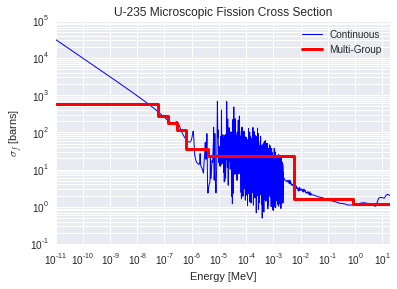
\includegraphics[width=0.8\linewidth]{figures/intro/u235-ce-mg-xs}
\caption[U-235 continuous energy and multi-group fission cross section]{U-235 continuous energy and 16-group fission cross section.}
\label{fig:chap1-u235-sigf}
\end{figure}

Many different engineering prescriptions have been developed to generate \ac{MGXS} for specific reactor configurations and spectra. In general, \ac{MGXS} generation schemes use a multi-level approach to decouple the energy, angular and spatial dimensions as depicted in Fig.~\ref{fig:chap1-multi-level-flow-chart}. The multi-level approach typically applies high-fidelity models of the energy self-shielding physics to low-fidelity geometric models of unique core components. The complexity of the energy treatment is then reduced at each level as larger and more complex geometric models are considered.

\begin{figure}
\centering
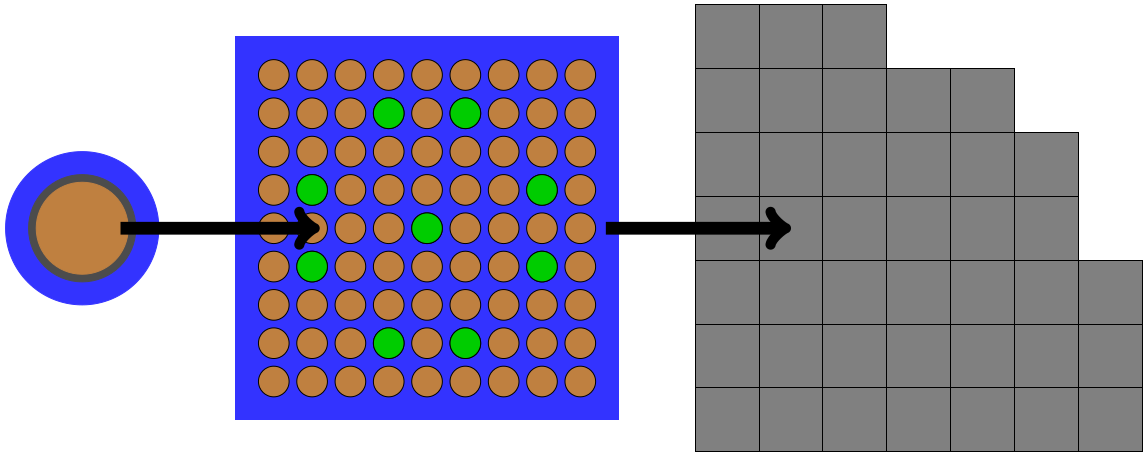
\includegraphics[width=0.9\linewidth]{figures/intro/multi-step-flow-chart}
\caption[Multi-level approach to reactor analysis]{Current multi-level framework for reactor analysis.}
\label{fig:chap1-multi-level-flow-chart}
\end{figure}

For example, the first stage for \ac{LWR} \ac{MGXS} generation attempts to capture energy self-shielding effects within simplified geometric models such as infinite fuel pin cells. This step typically condenses continuous energy cross sections to $\mathcal{O}(100)$ groups. These \ac{MGXS} are then used in a heterogenous lattice physics calculation of an individual fuel assembly within an infinite lattice. The lattice physics calculation models spatial self-shielding effects between pins of various material compositions and condenses the \ac{MGXS} to a coarse energy structure of $\mathcal{O}(10)$ groups. In addition, the \ac{MGXS} may be spatially-homogenized across the entire fuel assembly or across each fuel pin within each assembly. Finally, the spatially-homogenized coarse \ac{MGXS} for each fuel assembly are used in a whole-core calculation composed of many fuel assemblies.

The multi-level approach uses a combination of models of varying complexity to optimize overall simulation speed with accuracy. However, this is typically done at the sake of generality. For example, some prior knowledge of the neutron energy spectra is required to design approximations to the flux for a particular reactor configuration. Furthermore, multi-level \ac{MGXS} generation schemes do not generally model inter-assembly physics or the effect of reflectors and other core heterogeneities on the spatial distribution of the flux. Instead, geometric heuristcs are often used to embed spatial self-shielding effects in \ac{MGXS} for similarly shielded spatial zones (\textit{e.g.}, fuel pins). The approximations to the energy and spatial variation of the flux introduce approximation error in whole-core calculations and limit the space of core design parameters for which multi-level schemes may be applied. New reactor agnostic \ac{MGXS} generation methods are needed to enable deterministic transport-based methods to be as accurate and flexible as Monte Carlo in whole-core calculations.

%For reactors with a greater degree of spectral coupling, however, these approximations are not valid, resulting in ever larger datasets for the cross section generation process.

This thesis investigates the use of Monte Carlo methods to generate \ac{MGXS} for whole-core deterministic reactor analyis. Monte Carlo presents a natural approach to replace engineering prescriptions to approximate the flux with a stochastic approximation of the exact flux. The advantage of a \ac{MC}-based approach is that all of the relevant physics modeled in \ac{MC} may be directly embedded into \ac{MGXS}. This improvement in accuracy comes at the computational expense of converging group constant tallies to acceptably low uncertainties. \ac{MC} methods have increasingly been used to generate few group constants for coarse mesh diffusion, most notably by the Serpent \ac{MC} code~\cite{serpent2013manual}. However, there exist few rigorous and comprehensive analyses of \ac{MGXS} generation for heterogeneous fine mesh deterministic transport methods. 

\begin{emphbox}
\textbf{This thesis develops and evaluates \ac{MC}-based methods to generate \ac{MGXS} for fine mesh deterministic neutron transport codes.}
\end{emphbox}

In addition, \ac{MC}-based \ac{MGXS} generation methods to date have retained the multi-level geometric framework to tabulate \ac{MGXS} for individual reactor components -- such as infinite fuel pins and/or assemblies -- for subsequent use in whole-core multi-group calculations. Although the use of \ac{MC} within a multi-level scheme eliminates the need to approximate the flux in energy, it is does not account for spatial self-shielding effects throughout a reactor core. This thesis abandons the multi-level framework in place of a whole-core \ac{MC} calculation which simultaneously accounts for all energy and spatial self-shielding effects in a single step.

In theory, whole-core \ac{MC} calculations can be used to tally \ac{MGXS} in each spatial zone (\textit{e.g.}, 50,000+ fuel pins in a \ac{PWR} core) to account for the spatial variation in the flux. However, such simulations have not been employed for practical reasons -- in particular, the large memory footprint and computational expense of performing such calculations has been prohibitive for \ac{MC} codes until recent years. Furthermore, roughly the same number of particle histories would be required to converge the \ac{MGXS} tallies in each spatial zone as would be required for a direct whole-core calculation by \ac{MC}. Hence, it would be more useful to simply use \ac{MC} to compute the solution to the whole-core eigenvalue problem directly rather than use it to fully embed spatial self-shielding effects in \ac{MGXS} for deterministic transport codes. Therefore, in order for \ac{MC} to be practical for reactor agnostic fine mesh \ac{MGXS} generation, a new method is required to accelerate the convergence rate of the \ac{MGXS} tallies in each fine mesh region to a degree that is not possible for conventional whole-core Monte Carlo simulations. 

This thesis proposes to use statistical clustering methods to accelerate the convergence rate of whole-core \ac{MC} calculations for \ac{MGXS} generation. The novel approach developed in this work relies on the fact that many distinct spatial zones across a reactor core will experience similar if not identical spatial self-shielding effects, and therefore have similar if not identical \ac{MGXS}. The stochastic nature of \ac{MC} simulations will contribute statistical ``noise'' to the tally estimates for the \ac{MGXS}. As a result, the \ac{MGXS} estimates for similarly self-shielded spatial zones will form clusters which will converge as more particle histories are simulated. The goal of this thesis is to develop and apply algorithms to identify \ac{MGXS} clusters from ``noisy'' Monte Carlo tally data and to predict the true mean of each cluster prior to convergence. This methodology aims to generate \ac{MGXS} for deterministic neutron transport codes in a reactor agnostic and computationally efficient manner.

%The true mean of each cluster will then be used as the predicted estimate for the multi-group cross-section for each fine-mesh region in each cluster.

\begin{emphbox}
\textbf{This thesis uses statistical clustering algorithms to accelerate whole-core \ac{MC} calculations
which simultaneously model all energy- and spatial self-shielding effects for fine mesh \ac{MGXS} generation.}
\end{emphbox}


%%%%%%%%%%%%%%%%%%%%%%%%%%%%%%%%%%%%%%%%%%%%%%%%%%%%%%%%%%%%%%%%%%%%%%%%%%%%%%%
\section{Thesis Objectives}
\label{sec:chap1-objectives}

The subject matter of this thesis is organized along two main themes:

\begin{itemize}
\item \textbf{\textit{Approximation Error}} -- Quantify and diagnose approximation error(s) in \ac{MGXS} generated from \ac{MC} methods for simple heterogeous benchmark problems.
\item \textbf{\textit{Statistical Clustering}} -- Develop statistical clustering methods to accelerate the convergence rate of \ac{MGXS} on heterogeneous \ac{MC} tally meshes.
\end{itemize}

The first theme of this thesis rigorously assesses the efficacy of \ac{MGXS} generation with \ac{MC} for fine mesh transport calculations. Some of the approximations made by \ac{MC}-based \ac{MGXS} generation are quantified, including the energy- and spatial-dependence of condensed \ac{MGXS}. An in-depth analysis of systematic bias resulting from constant-in-angle total \ac{MGXS} is presented, along with a scheme based on \ac{SPH} factors to compensate for this loss in accuracy. 

The second theme of this thesis develops a new methodology to simultaneously capture local and global spatial self-shielding effects in \ac{MGXS} for whole-core calcuations. This scheme applies statistical clustering methods to accelerate the convergence rate of \ac{MGXS} tallied on fine, heterogeneous spatial meshes in Monte Carlo. The latent variable model which inspires the clustering paradigm is presented, along with a discussion of the implementation of a data pipeline to evaluate clustering algorithms for \ac{MGXS} generation. A series of increasingly complex heterogeneous benchmarks are modeled to empirically compare the accuracy and convergence rate of the approach with more traditional multi-level schemes for \ac{MC}-based MGXS generation.


%%%%%%%%%%%%%%%%%%%%%%%%%%%%%%%%%%%%%%%%%%%%%%%%%%%%%%%%%%%%%%%%%%%%%%%%%%%%%%%
\section{Thesis Outline}
\label{sec:chap1-outline}

This thesis is segmented into five Parts. Part I is comprised of this introductory chapter.

Part II discusses the relevant background information for this thesis. Chap.~\ref{chap:mgxs} reviews multi-group neutron transport theory and considers some common approximations made in \ac{MGXS} generation and multi-group transport codes. Chap.~\ref{chap:mgxs-mc} introduces Monte Carlo as an approach to generate \ac{MGXS}, and highlights relevant studies in the literature which have used \ac{MC} to generate \ac{MGXS}. Chap.~\ref{chap:workflow} presents the simulation workflow developed for this thesis to evaluate \ac{MC} for \ac{MGXS} generation, including the OpenMC, OpenMOC and OpenCG codes.

Part III diagnoses common sources of approximation error in \ac{MGXS} generation and multi-group transport methods. Chap. \ref{chap:biases} quantifies the impact of multi-group approxmation error for simple, heterogeneous \ac{PWR} geometries. Chap.~\ref{chap:sph} presents an algorithmic approach to mitigate systematic biases resulting from constant-in-angle total \ac{MGXS} using \ac{SPH} factors, and motivates the need for future work to address this issue.

Part IV develops a novel approach based on statistical clustering methods to accelerate whole-core \ac{MC} calculations for \ac{MGXS} generation. Chap.~\ref{chap:benchmarks} analyzes the convergence rate of \ac{MGXS} datasets computed on fine spatial \ac{MC} tally meshes for a series of heterogeneous \ac{PWR} benchmark models to motivate this new methodology. Chap.~\ref{chap:quantify} quantifies the impact of using \ac{MGXS} which reflect inter-pin and inter-assembly spatial self-shielding effects on the solutions computed by multi-group deterministic transport methods. Chap.~\ref{chap:spatial} analyzes the emergence of \ac{MGXS} clusters due to spatial self-shielding with a variety of visual aids. Chap.~\ref{chap:unsupervised} outlines a latent variable model for clustering \ac{MGXS}, along with a data pipeline for unsupervised clustering to accelerate the \ac{MGXS} convergence rate. Chapter~\ref{chap:results} evaluates the impact of clustered \ac{MGXS} on the accuracy and convergence rate of the eigenvalue solutions computed by deterministic transport methods.

Part V is composed of Chapter~\ref{chap:conclusions} which summarizes the progress made in this thesis to chart a path forward for \ac{MC}-based \ac{MGXS} generation for whole-core deterministic transport methods.

%\begin{figure}
%\begin{subfigure}{\textwidth}
%  \centering
%  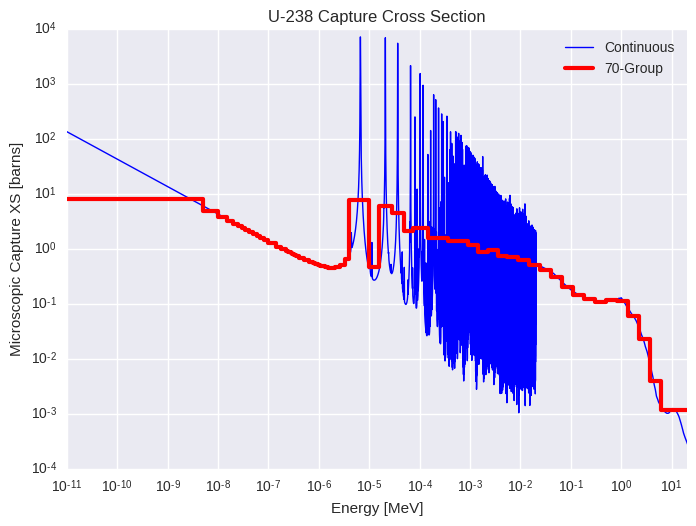
\includegraphics[width=0.9\linewidth]{figures/intro/u238-capture-70}
%  \caption{}
%\end{subfigure}
%\begin{subfigure}{\textwidth}
%  \centering
%  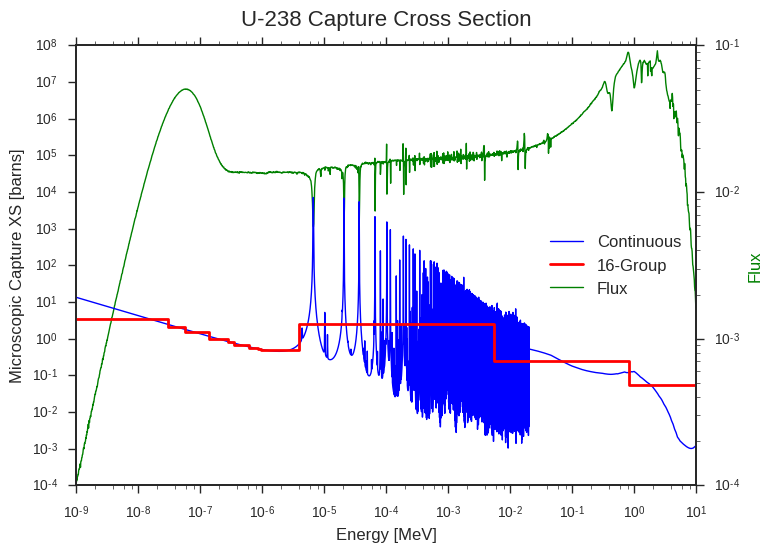
\includegraphics[width=0.9\linewidth]{figures/intro/u238-capture-16}
%  \caption{}
%\end{subfigure}
%\caption[Uranium-238 capture cross section]{Continuous energy and multi-group cross sections for U-238 capture in a PWR spectrum for 70-groups (a) and 16-groups (b).}
%\label{fig:pwr-ce-mg-xs}
%\end{figure}



\part{Background}
\chapter{Approximations in Multi-Group Transport Theory}
\label{chap:mgxs}

This chapter presents an overview of some of the approximations made by methods which solve the multi-group form of the neutron transport equation. This chapter begins by reviewing the continuous energy steady-state neutron transport equation in Sec.~\ref{sec:chap2-background}. The following sections present simplifications to the angular (Sec.~\ref{sec:chap2-approx-angle}), energy (Sec.~\ref{sec:chap2-approx-energy}) and spatial dependence (Sec.~\ref{sec:chap2-approx-space}) of the equation. The approximations are not specific to a particular approach for solving the transport equation and may be employed by either stochastic or deterministic methods. Sec.~\ref{sec:chap2-mgxs-lib} concludes with a discussion of how these approximations present challenges for accurate \ac{MGXS} generation.


%%%%%%%%%%%%%%%%%%%%%%%%%%%%%%%%%%%%%%%%%%%%%%%%%%%%%%%%%%%%%%%%%%%%%%%%%%%%%%%
\section{Background}
\label{sec:chap2-background}

The field of reactor physics is concerned with computing the distribution of nuclear reaction rates throughout a nuclear reactor core. Nuclear reaction rates are dependent on two fundamental quantities: the density of neutrons and the probability of interaction. The angular neutron flux $\psi(\mathbf{r},\mathbf{\Omega},E)$ models the neutron density\footnote{Unlike the common definition of flux used in other areas of science and engineering, the angular flux $\psi$ is the product of the volume density and speed of neutrons in phase space.} as the path length traveled by neutrons per unit volume and is dependent on a neutron's spatial position $\mathbf{r}$, direction of motion $\mathbf{\Omega}$ and energy $E$\footnote{Vector-valued quantities are expressed in boldface font.}$^{,}$\footnote{This thesis focuses on steady-state calculations and time dependence is neglected for simplicity.}. The macroscopic cross section $\Sigma_{x}(\mathbf{r},E)$ is defined as the probability of interaction $x$ per unit of length traveled by a neutron at some position and energy. A reaction rate $\mathcal{R}_{x}$ can be simply computed as the product of the angular flux and cross section:

\begin{dmath}
\label{eqn:chap2-rxn-rates}
\mathcal{R}_{x}(\mathbf{r},\mathbf{\Omega},E) = \Sigma_{x}(\mathbf{r},E) \psi(\mathbf{r},\mathbf{\Omega},E)
\end{dmath}

\noindent The macroscopic cross section $\Sigma_{x}$ is proportional to a quantity known as the microscopic cross section $\sigma_{x}$. The microscopic cross section is a property of a particular nuclide and is measured experimentally for various reaction types $x$ which include fission $f$, radiative capture $\gamma$ and scattering $s$\footnote{Scattering as defined here includes both inelastic and elastic scattering channels.}. The macroscopic cross section is the sum of the microscopic cross sections of each nuclide $i$ weighted by its number density $N_{i}$:

\begin{dmath}
\label{eqn:chap2-macro-xs-sum}
\Sigma_{x}(\mathbf{r},E) = \sum_{i}N_{i}(\mathbf{r})\sigma_{i,x}(E)
\end{dmath}

The microscopic cross section is highly dependent on the energy of the incoming neutron. As illustrated in Fig.~\ref{fig:chap2-u238-xs}, a cross section varies several orders of magnitude within an energy interval on the order of an eV near nuclear resonances. The probability of some interactions also depend on other properties which characterize the output channel of the reaction. For example, the scattering cross section $\sigma_{s}$ depends on the energy and direction of motion of the outgoing neutron. The macroscopic cross section varies in space when nuclide densities depend on the position within a heterogeneous system.

\begin{figure}[H]
  \centering
  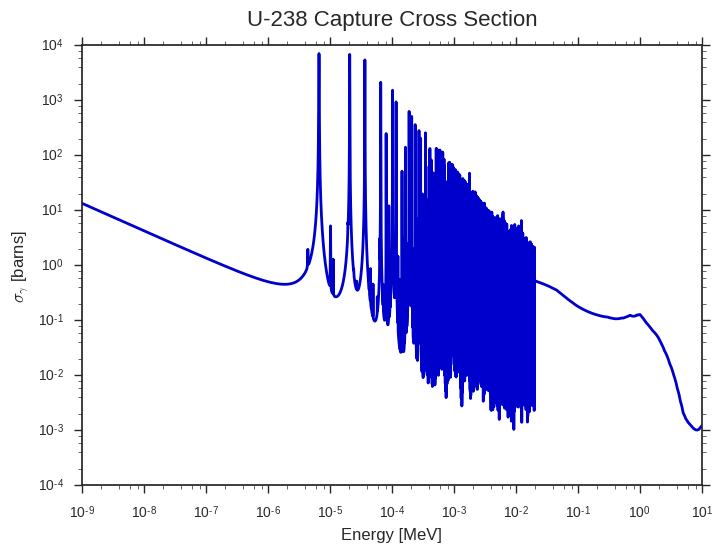
\includegraphics[width=0.8\linewidth]{figures/mgxs/u238-capture-xs}
\caption[U-238 capture cross section]{The continuous energy capture cross section for U-238.}
\label{fig:chap2-u238-xs}
\end{figure}
 
Although cross sections are experimentally measured, the neutron flux must be calculated analytically or with simulation. The steady-state Boltzmann transport equation~\cite{bell1970nuclear} is integro-differential in the neutron angular flux $\psi(\mathbf{r},\mathbf{\Omega},E)$ and balances the rate of change of the population of neutrons in phase space to the difference between the production and loss rates of neutrons within a closed system:

\begin{dmath}
\label{eqn:chap2-transport-ce}
\mathbf{\Omega} \cdot \nabla \psi(\mathbf{r},\mathbf{\Omega},E) + \Sigma_{t}(\mathbf{r},E)\psi(\mathbf{r},\mathbf{\Omega},E) \;\;\;\;\; = \;\;\;\;\; \int\displaylimits_{0}^{\infty}\int\displaylimits_{4\pi} \Sigma_{s}(\mathbf{r},{\mathbf{\Omega'}\rightarrow\mathbf{\Omega}},{E'\rightarrow E}) \psi(\mathbf{r},\mathbf{\Omega'},E') \mathrm{d}\mathbf{\Omega'} \mathrm{d}E' + Q(\mathbf{r},\mathbf{\Omega},E)
\end{dmath}

The first term on the left hand side of the equation represents the streaming of neutrons within space and the second term is the total neutron collision rate determined by the total cross section $\Sigma_{t}$. On the right hand side, the first term models the scattering of neutrons at some energy $E'$ and direction $\mathbf{\Omega'}$ into energy $E$ and direction $\mathbf{\Omega}$. The final term represents a generic source $Q$ of neutrons. In the case of critical systems, such as nuclear reactors, $Q$ is a source of fission neutrons:

\begin{dmath}
\label{eqn:chap2-source}
Q(\mathbf{r},\mathbf{\Omega},E) = \frac{1}{k_{eff}}\int\displaylimits_{0}^{\infty}\int\displaylimits_{4\pi} \nu\Sigma_{f}(\mathbf{r},{\mathbf{\Omega'}\rightarrow \mathbf{\Omega}},{E'\rightarrow E})\psi(\mathbf{r},\mathbf{\Omega'},E') \mathrm{d}\mathbf{\Omega'} \mathrm{d}E'
\end{dmath}

\noindent The fission production cross section $\nu\Sigma_{f}$ represents the probability of neutrons emitted at energy $E$ and angle $\mathbf{\Omega}$ resulting from fission events precipitated by neutrons at $E'$ and $\mathbf{\Omega'}$. The eigenvalue $k_{eff}$ of a critical system represents the multiplication of neutrons from fission and forces balance between neutron sources and losses due to absorption and leakage.

A solution for the neutron flux must computed from the transport equation in order to compute reaction rate distributions. The accurate determination of the neutron flux is primarily challenged by  the complicated energy structure of the cross sections. In addition, the distribution of neutrons in \ac{LWR}s spans 11 orders of magnitude from a few MeV at birth from fission emission to death by absorption at energies as low as 10$^{-5}$ eV. As a result, analytical solutions to Eqn.~\ref{eqn:chap2-transport-ce} are intractable without significant simplifying assumptions.

Instead, numerical simulation is used to solve the transport equation for the flux. Monte Carlo may be employed to exactly treat the energy dependence in Eqn.~\ref{eqn:chap2-transport-ce}\footnote{The treatment is only as exact as the uncertainties in measured nuclear cross section data will permit.}, but it is computationally burdensome and impractical for routine nuclear reactor analysis. Although space and angle may be discretized using standard techniques for the solution of partial differential equations, special treatment must be given to the energy variable. The following sections introduce approximations used to reduce the dimensionality of the equation to permit tractable multi-group calculations.

\begin{emphbox}
\textbf{Nuclear reactor simulations calculate the neutron multiplication factor $k_{eff}$ and reaction rate spatial distributions. Monte Carlo methods are the most accurate approach, but are not yet practical for whole-core analysis.}
\end{emphbox}

%The following sections present standard approximations made in multi-group theory to reduce the dimensionality of the angular, energy and spatial variables 


%%%%%%%%%%%%%%%%%%%%%%%%%%%%%%%%%%%%%%%%%%%%%%%%%%%%%%%%%%%%%%%%%%%%%%%%%%%%%%%
\section{Approximations in Angle}
\label{sec:chap2-approx-angle}

%%%%%%%%%%%%%%%%%%%%%%%%%%%
\subsection{Isotropic Fission Source}
\label{subsec:chap2-fiss-src}

The neutrons emitted from fission form a nearly isotropic distribution independent of the energy or angle of the incoming neutron\footnote{This approximation is only valid for a large number of fission events as is the case in a nuclear reactor.}. As a result, the fission production cross section can be approximated as $\nu\Sigma_{f}(\mathbf{r},{\mathbf{\Omega'}\rightarrow \mathbf{\Omega}},{E'\rightarrow E}) \approx \nu\Sigma_{f}(\mathbf{r},{E'\rightarrow E})$. This permits the fission source in Eqn.~\ref{eqn:chap2-source} to be written as:

\begin{dmath}
\label{eqn:chap2-source-scalar-flux}
Q(\mathbf{r},\mathbf{\Omega},E) = \frac{1}{4\pi k_{eff}}\int\displaylimits_{0}^{\infty}\int\displaylimits_{4\pi} \nu\Sigma_{f}(\mathbf{r},{E'\rightarrow E})\psi(\mathbf{r},\mathbf{\Omega},E') \mathrm{d}\mathbf{\Omega} \mathrm{d}E'
\end{dmath}

\noindent This expression may be further simplified in terms of the scalar neutron flux $\phi(\mathbf{r},E)$:

\begin{dmath}
\label{eqn:chap2-source-scalar-flux}
Q(\mathbf{r},\mathbf{\Omega},E) = \frac{1}{4\pi k_{eff}} \int\displaylimits_{0}^{\infty}\nu\Sigma_{f}(\mathbf{r},{E'\rightarrow E})\phi(\mathbf{r},E') \mathrm{d}E'
\end{dmath}

\begin{dmath}
\label{eqn:chap2-scalar-flux}
\phi_{g}(\mathbf{r},E) = \int\displaylimits_{4\pi}\psi(\mathbf{r},\mathbf{\Omega},E)\mathrm{d}\mathbf{\Omega}
\end{dmath}

\noindent The isotropic approximation reduces the dimensionality of the fission production term in the transport equation and simplifies the derivation of the approximations in the following sections.


%%%%%%%%%%%%%%%%%%%%%%%%%%%%%%
\subsection{Angular Expansion of the Scattering Kernel}
\label{subsec:chap2-scatt-src}

Unlike the fission source, the source of neutrons from scattering cannot be treated as isotropic since it is strongly dependent on the relationship between the incoming and outgoing directions of motion. The dimensionality of the scattering source term in the transport equation -- known as the double differential scattering kernel -- is commonly reduced with basis function expansions in angle~\cite{hebert2009applied, cacuci2010handbook}. The angular flux is first expanded as an infinite sum of spherical harmonic functions $Y_{\ell}^{m}(\mathbf{\Omega})$ and angular flux moments $\psi_{\ell}^{m}(\mathbf{r},E)$:

\begin{dmath}
\label{eqn:chap2-flux-expand}
\psi(\mathbf{r},\mathbf{\Omega},E) = \displaystyle\sum\limits_{\ell=0}^{\infty} \frac{2\ell+1}{4\pi} \displaystyle\sum\limits_{m=-\ell}^{\ell} \psi_{\ell}^{m}(\mathbf{r},E)Y_{l}^{m}(\mathbf{\Omega})
\end{dmath}

\begin{dmath}
\label{eqn:chap2-flux-moment}
\psi_{\ell}^{m}(\mathbf{r},E) = \displaystyle\int\limits_{4\pi} \psi(\mathbf{r},\mathbf{\Omega},E)Y_{\ell}^{m}(\mathbf{\Omega}) \mathrm{d}\mathbf{\Omega}
\end{dmath}

Similarly, the angular dependence of the scattering cross section $\Sigma_{s}(\mathbf{r},{\mathbf{\Omega'}\rightarrow\mathbf{\Omega}},{E'\rightarrow E})$ can be treated with a basis function expansion. The scattering cross section can be simplified without approximation by noting that the distribution over the change in direction $\mu$ is independent of the incoming angle $\mathbf{\Omega'}$ in isotropic media. The re-parametrized scattering cross section $\Sigma_{s}(\mathbf{r},\mu,E'\rightarrow E)$ can then expanded as an infinite sum of Legendre polynomials $P_{\ell}(\mu)$ and scattering moments $\Sigma_{s,\ell}(\mathbf{r},{E'\rightarrow E})$:

\begin{dmath}
\label{eqn:chap2-scatt-expand}
\Sigma_{s}(\mathbf{r},\mu,E'\rightarrow E) = \displaystyle\sum\limits_{\ell=0}^{\infty} \frac{2\ell+1}{2} \Sigma_{s,\ell}(\mathbf{r},{E'\rightarrow E})P_{\ell}(\mu)
\end{dmath}

\begin{dmath}
\label{eqn:chap2-scatt-moment}
\Sigma_{s,\ell}(\mathbf{r},E'\rightarrow E) = \displaystyle\int\limits_{-1}^{1} \Sigma_{s}(\mathbf{r},\mu,{E'\rightarrow E})P_{\ell}(\mu)\mathrm{d}\mu
\end{dmath}

The expansions of the angular flux in spherical harmonics and the scattering cross section in Legendre polynomials may be substituted into the scattering kernel. The spherical harmonic addition theorem can be applied to simplify the kernel in terms of only the real components $R_{\ell}^{m}(\mathbf{\Omega})$ of the spherical harmonics:

\begin{dmath}
\label{eqn:chap2-scatt-src-expand}
\int\displaylimits_{0}^{\infty}\int\displaylimits_{4\pi} \Sigma_{s}(\mathbf{r},{\mathbf{\Omega'}\rightarrow\mathbf{\Omega}},{E'\rightarrow E}) \psi(\mathbf{r},\mathbf{\Omega'},E') \mathrm{d}\mathbf{\Omega'} \mathrm{d}E' = \int\displaylimits_{0}^{\infty} \displaystyle\sum\limits_{\ell=0}^{\infty} \frac{2\ell+1}{4\pi} \Sigma_{s,\ell}(\mathbf{r},{E'\rightarrow E}) \psi_{\ell}^{m}(\mathbf{r},E')R_{\ell}^{m}(\mathbf{\Omega}) \mathrm{d}E'
\end{dmath}

No approximation has been made to the scattering kernel's angular dependence in Eqn.~\ref{eqn:chap2-scatt-src-expand}. In practice, however, the expansion is truncated to a finite number of spherical harmonics $L$ to make the transport equation computationally tractable. The transport equation with the scattering source expansion and isotropic fission source is then:

\begin{dmath}
\label{eqn:chap2-transport-ce-2}
\mathbf{\Omega} \cdot \nabla \psi(\mathbf{r},\mathbf{\Omega},E) + \Sigma_{t}(\mathbf{r},E)\psi(\mathbf{r},\mathbf{\Omega},E) = \int\displaylimits_{0}^{\infty} \displaystyle\sum\limits_{\ell=0}^{L} \frac{2\ell+1}{4\pi} \displaystyle\sum\limits_{m=-\ell}^{\ell} \Sigma_{s,\ell}(\mathbf{r},{E'\rightarrow E}) \psi_{\ell}^{m}(\mathbf{r},E')R_{\ell}^{m}(\mathbf{\Omega}) \mathrm{d}E' + \frac{1}{4\pi k_{eff}}\int\displaylimits_{0}^{\infty} \nu\Sigma_{f}(\mathbf{r},{E'\rightarrow E})\phi(\mathbf{r},E')\mathrm{d}E'
\end{dmath}


%%%%%%%%%%%%%%%%%%%%%%%%%%%%%%
\subsection{Transport Correction}
\label{subsec:chap2-transport-corr}

The scattering matrix and flux moments substantially increase the memory and storage requirements for calculation schemes which model anisotropic scattering with a finite moment expansion as introduced in Sec.~\ref{subsec:chap2-scatt-src}. In practice, many methods attempt to implicitly model anisotropic scattering effects with transport corrected cross sections. These approaches seek to define a correction which makes the transport equation with isotropic scattering in the laboratory system ($L=0$) equivalent to the general equation with anisotropic scattering. Various transport corrections are thoroughly detailed in the TRANSX~\cite{macfarlane1993transx} and NJOY~\cite{macfarlane2000njoy} manuals, each of which follow the approach taken by Bell, Hansen and Sandmeier in~\cite{bell1967transport}. This section summarizes the derivation in~\cite{hebert2009applied}.

First, consider a truncated form of the Legendre polynomial expansion of the scattering cross section $\Sigma_{s}(\mathbf{r},\mu,E'\rightarrow E)$ in Eqn.~\ref{eqn:chap2-scatt-expand}:

\begin{dmath}
\label{eqn:chap2-scatt-expand-truncate}
\Sigma_{s}(\mathbf{r},\mu,E'\rightarrow E) = \displaystyle\sum\limits_{\ell=0}^{\infty} \frac{2\ell+1}{2} \Sigma_{s,\ell}(\mathbf{r},{E'\rightarrow E})P_{\ell}(\mu) \approx \displaystyle\sum\limits_{\ell=0}^{L} \frac{2\ell+1}{2} \tilde{\Sigma}_{s,\ell}(\mathbf{r},{E'\rightarrow E})P_{\ell}(\mu) + \Delta\Sigma_{tr}(\mathbf{r},{E'\rightarrow E})\delta(\mu-1)
\end{dmath}

\noindent where $\tilde{\Sigma}_{s,\ell}$ is a modified form of the scattering moment $\Sigma_{s,\ell}$ and $\Delta\Sigma_{tr}$ is a transport correction term. The Kronecker delta function $\delta(\mu-1)$ is used to make the correction term forward peaked in order to best capture the first order anisotropies in thermal reactors. The coefficients $\tilde{\Sigma}_{s,\ell}$ and $\Delta\Sigma_{tr}$ are defined such that the Legendre moments of the scattering cross section in Eqn.~\ref{eqn:chap2-scatt-moment} are preserved for $0 \le \ell \le L+1$:

\begin{dmath}
\label{eqn:chap2-scatt-moment-preserve}
\Sigma_{s,\ell}(\mathbf{r},E'\rightarrow E) = \displaystyle\int\limits_{-1}^{1} \Sigma_{s}(\mathbf{r},\mu,{E\rightarrow E})P_{\ell}(\mu)\mathrm{d}\mu \approx \displaystyle\int\limits_{-1}^{1} \displaystyle\sum\limits_{\ell'=0}^{L} \frac{2\ell'+1}{2} \tilde{\Sigma}_{s,\ell'}(\mathbf{r},{E'\rightarrow E})P_{\ell'}(\mu)P_{\ell}(\mu)\mathrm{d}\mu + \displaystyle\int\limits_{-1}^{1} \Delta\Sigma_{tr}(\mathbf{r},{E'\rightarrow E})\delta(\mu-1)P_{\ell}(\mu)\mathrm{d}\mu
\end{dmath}

The following simultaneous system of equalities for $0 \le \ell \le L$ follows from the identity $P_{\ell}(1) = 1$ and the orthogonality relation of the Legendre polynomial basis set:

\begin{dmath}
\label{eqn:chap2-sigsl}
\tilde{\Sigma}_{s,\ell}(\mathbf{r},{E'\rightarrow E}) + \Delta\Sigma_{tr}(\mathbf{r},{E'\rightarrow E}) = \Sigma_{s,\ell}(\mathbf{r},{E'\rightarrow E})
\end{dmath}

\begin{dmath}
\label{eqn:chap2-delta-transport}
\Delta\Sigma_{tr}(\mathbf{r},{E'\rightarrow E}) = \Sigma_{s,L+1}(\mathbf{r},{E'\rightarrow E})
\end{dmath}

\noindent For isotropic in lab scattering with $L = 0$ the Eqns.~\ref{eqn:chap2-scatt-expand-truncate} and~\ref{eqn:chap2-delta-transport} simplify in terms of only the zeroth and first order scattering moments:

\begin{dmath}
\label{eqn:chap2-iso-scatt-kernel-transport}
\Sigma_{s}(\mathbf{r},\mu,E'\rightarrow E) \approx \frac{1}{2}\left[\Sigma_{s,0}(\mathbf{r},{E'\rightarrow E}) - \Sigma_{s,1}(\mathbf{r},{E'\rightarrow E})\right] + \Sigma_{s,1}(\mathbf{r},{E'\rightarrow E})\delta(\mu-1)
\end{dmath}

\noindent The transport-corrected scattering cross section in Eqn.~\ref{eqn:chap2-iso-scatt-kernel-transport} is then substituted into the transport equation in Eqn.~\ref{eqn:chap2-transport-ce-2} with an isotropic scattering kernel and rearranged to produce:

\begin{dmath}
\label{eqn:chap2-transport-ce-3}
\mathbf{\Omega} \cdot \nabla \psi(\mathbf{r},\mathbf{\Omega},E) + \Sigma_{t}(\mathbf{r},E)\psi(\mathbf{r},\mathbf{\Omega},E) - \int\displaylimits_{0}^{\infty} \Sigma_{s,1}(\mathbf{r},{E'\rightarrow E})\phi(\mathbf{r},E')\mathrm{d}E' = \frac{1}{4\pi} \int\displaylimits_{0}^{\infty} \left[\Sigma_{s,0}(\mathbf{r},{E'\rightarrow E}) - \Sigma_{s,1}(\mathbf{r},{E'\rightarrow E})\right] \phi(\mathbf{r},E')\mathrm{d}E' + \frac{1}{4\pi k_{eff}}\int\displaylimits_{0}^{\infty}\nu\Sigma_{f}(\mathbf{r},{E'\rightarrow E})\phi(\mathbf{r},E') \mathrm{d}E'
\end{dmath}

\noindent where the relation $\phi = \psi_{0}^{0}$ for the scalar flux has been used to completely remove the angular dependence from the isotropic scattering kernel. The transport correction term $\Delta\Sigma_{tr}(\mathbf{r},E)$ can be defined such that it can be lumped into new transport-corrected total and scattering cross sections $\tilde{\Sigma}_{t}$ and $\tilde{\Sigma}_{s}$ as follows:

\begin{dmath}
\label{eqn:chap2-transport-xs}
\Delta\Sigma_{tr}(\mathbf{r},E) \equiv \frac{\int\displaylimits_{0}^{\infty} \Sigma_{s,1}(\mathbf{r},{E'\rightarrow E})\phi(\mathbf{r},E') \mathrm{d}E'}{\phi(\mathbf{r},E)}
\end{dmath}

\begin{dmath}
\label{eqn:chap2-transpot-corr-tot-x}
\tilde{\Sigma}_{t}(\mathbf{r},E) = \Sigma_{t}(\mathbf{r},E) - \Delta\Sigma_{tr}(\mathbf{r},E)
\end{dmath}

\begin{dmath}
\label{eqn:chap2-transpot-corr-scatt-x}
\tilde{\Sigma}_{s}(\mathbf{r},{E'\rightarrow E}) = \Sigma_{s,0}(\mathbf{r},{E'\rightarrow E}) - \Delta\Sigma_{tr}(\mathbf{r},E)\delta(E'-E)
\end{dmath}

This definition of the transport correction is termed the \textit{in-scatter approximation} in the literature~\cite{yamamoto2008simplified}. Finally, the transport equation in Eqn.~\ref{eqn:chap2-transport-ce-3} can be simplified with the substitution of the corrected total and scattering cross sections:

\begin{dmath}
\label{eqn:chap2-transport-ce-4}
\mathbf{\Omega} \cdot \nabla \psi(\mathbf{r},\mathbf{\Omega},E) + \tilde{\Sigma}_{t}(\mathbf{r},E)\psi(\mathbf{r},\mathbf{\Omega},E) = \frac{1}{4\pi} \int\displaylimits_{0}^{\infty} \tilde{\Sigma}_{s}(\mathbf{r},{E'\rightarrow E}) \phi(\mathbf{r},E') \mathrm{d}E' + \frac{1}{4\pi k_{eff}}\int\displaylimits_{0}^{\infty} \nu\Sigma_{f}(\mathbf{r},{E'\rightarrow E})\phi(\mathbf{r},E') \mathrm{d}E'
\end{dmath}

%This is the form of the transport equation that will be used throughout the remainder of this chapter. 

%The approximations in energy and space that will be introduced in the following sections are directly applicable to the transport equation with explicit treatment of anisotropic scattering with a moment expansion as given in Eqn.~\ref{eqn:chap2-transport-ce-2}.

%The angular flux expansion can be substituted into the total collision terminto the total collision term in the transport equation:

%\begin{dmath}
%\label{eqn:chap2-tot-expand}
%\Sigma_{t}(\mathbf{r},E)\psi(\mathbf{r},\mathbf{\Omega},E) = \displaystyle\sum\limits_{\ell=0}^{\infty} \frac{2\ell+1}{4\pi} \displaystyle\sum\limits_{m=-\ell}^{\ell} \Sigma_{t,\ell}^{m}(\mathbf{r},E) \psi_{\ell}^{m}(\mathbf{r},E)Y_{l}^{m}(\mathbf{\Omega})
%\end{dmath}

%\begin{dmath}
%\label{eqn:chap2-tot-moment}
%\Sigma_{t,\ell}^{m}(\mathbf{r},E) = \frac{\Sigma_{t}(\mathbf{r},E)\psi_{\ell}^{m}(\mathbf{r},E)}{\psi_{\ell}^{m}(\mathbf{r},E)}
%\end{dmath}

%model scattering as isotropic in the laboratory system (equivalent to truncating the scattering kernel with $L = 0$) and define a transport correction which makes the transport equation equivalent to one with anisotropic scattering

%The expanded total collision term in Eqn.~\ref{eqn:chap2-tot-expand} can be moved to the right hand side of Eqn.~\ref{eqn:chap2-transport-ce-2}, and with some simplifications, incorporated into the scattering kernel expansion. A new free parameter for the transport-corrected total cross section $\Sigma_{tr}$ is then added as a reaction rate to each side of the transport equation, where the spatial and energy variables have been dropped for simplicity:

%\begin{dmath}
%\label{eqn:chap2-transport-ce-3}
%\mathbf{\Omega} \cdot \nabla \psi + \Sigma_{tr}\psi = \int\displaylimits_{0}^{\infty} \displaystyle\sum\limits_{\ell=0}^{L} \frac{2\ell+1}{4\pi} \displaystyle\sum\limits_{m=-\ell}^{\ell} \left(\Sigma_{s,\ell} - \left(\Sigma_{t,\ell}^{m} - \Sigma_{tr}\right)\delta_{E',E}\right) \psi_{\ell}^{m}R_{\ell}^{m}(\mathbf{\Omega}) \mathrm{d}E' + \frac{1}{4\pi k_{eff}}\int\displaylimits_{0}^{\infty}\int\displaylimits_{4\pi} \nu\Sigma_{f}\psi \mathrm{d}\mathbf{\Omega'} \mathrm{d}E'
%\end{dmath}

%The scattering kernel expansion has been truncated to order $L$ and the variable $\delta_{E',E}$ is the Kronecker delta function. A variety of forms for the transport cross section $\Sigma_{tr}$ are extensively discussed in the literature. One of the most commonly used versions of $\Sigma_{tr}$ is known as the \textit{in-scatter approximation}~\cite{yamamoto2008simplified}. In the case of isotropic scattering where $L = 0$, the in-scatter approximation is defined as the total cross section with a current-weighted correction term based on $\Sigma_{s,\ell=1}$:

%This form is Each of these forms are presented here for the case of isotropic scattering where $L = 0$, as is a common scenario in many deterministic transport codes.

%\begin{dmath}
%\label{eqn:chap2-transport-in-scatt-curr}
%\Sigma_{tr}(\mathbf{r},E) \equiv \Sigma_{t}(\mathbf{r},E) - \frac{\int\limits_{0}^{\infty}\Sigma_{s,\ell=1}(\mathbf{r},{E'\rightarrow E})\psi_{1}(\mathbf{r},E')\mathrm{d}E'}{\psi_{1}(\mathbf{r},E)}
%\end{dmath}

%Since it is generally impractical to compute the neutron current \textit{a priori}, the first moment of the flux -- known as the scalar flux $\phi$ -- is more commonly used to weight the correction term:

%In-scatter approximation with scalar flux weighting - make the approximation that weighting with the current $\psi_{1}$ is akin to weighting with the scalar flux $\psi_{0}$:

%\begin{dmath}
%\label{eqn:chap2-transport-in-scatt-flux}
%\Sigma_{tr}(\mathbf{r},E) \equiv \Sigma_{t}(\mathbf{r},E) - \frac{\int\limits_{0}^{\infty}\Sigma_{s,\ell=1}(\mathbf{r},{E'\rightarrow E})\psi_{0}(\mathbf{r},E')\mathrm{d}E'}{\psi_{0}(\mathbf{r},E)}
%\end{dmath}

%Out-scatter approximation:

%\begin{dmath}
%\label{eqn:chap2-transport-out-scatt}
%\Sigma_{tr}(\mathbf{r},E) \equiv \Sigma_{t}(\mathbf{r},E) - \int\limits_{0}^{\infty}%\Sigma_{s,\ell=1}(\mathbf{r},{E'\rightarrow E})\mathrm{d}E'
%\end{dmath}

%Although some deterministic transport codes explicitly treat the anisotropy of the scattering source with a finite moment expansion, it is common for many methods to assume isotropic scattering and model the first term in the expansion in terms of the scalar neutron flux $\phi$:

%\begin{dmath}
%\label{eqn:chap2-scatt-src-iso}
%\int\displaylimits_{0}^{\infty}\int\displaylimits_{4\pi} \Sigma_{s}(\mathbf{r},{\mathbf{\Omega'}\rightarrow\mathbf{\Omega}},{E'\rightarrow E}) \psi(\mathbf{r},\mathbf{\Omega'},E') \mathrm{d}\mathbf{\Omega'} \mathrm{d}E' \approx \frac{1}{4\pi} \int\displaylimits_{0}^{\infty} \Sigma_{s}(\mathbf{r},{E'\rightarrow E}) \psi_{0}(\mathbf{r},E') = \frac{1}{4\pi} \int\displaylimits_{0}^{\infty} \Sigma_{s,0}(\mathbf{r},{E'\rightarrow E}) \phi(\mathbf{r},E') \mathrm{d}E'
%\end{dmath}

%\begin{dmath}
%\label{eqn:chap2-source-scalar-flux}
%\phi(\mathbf{r},E) = \int\displaylimits_{4\pi}\psi(\mathbf{r},\mathbf{\Omega'},E) \mathrm{d}\Omega'
%\end{dmath}

\begin{emphbox}
\textbf{The neutron fission source is isotropic in reactors. The scattering source is simplified with a basis function expansion in angle. A transport correction is commonly used to account for anisotropic scattering in simulations that simplify the scattering source as isotropic.}
\end{emphbox}


%%%%%%%%%%%%%%%%%%%%%%%%%%%%%%%%%%%%%%%%%%%%%%%%%%%%%%%%%%%%%%%%%%%%%%%%%%%%%%%
\section{Approximations in Energy}
\label{sec:chap2-approx-energy}

%%%%%%%%%%%%%%%%%%%%%%%%%%%%%%%%%%
\subsection{Energy Discretization}
\label{subsec:chap2-energy}

The multi-group approach used to solve the transport equation subdivides the neutron's energy into discrete bins known as energy groups. The energy groups are indexed starting at 1 for high energies and ending with $G$ for the lowest energies of interest. An energy group $g \in \left\{1, 2, \ldots, G\right\}$ spans a range of energies from $\left[E_{g}, E_{g-1}\right]$ where $E_{0}$ is the highest energy under consideration and $E_{g}$ is the upper bound of group $g$\footnote{This convention derives from the fact that neutrons are emitted at high energies from fission and are absorbed at lesser energies in \ac{LWR}s.}. First, a group-wise angular flux $\psi_{g}$ and scalar flux $\phi_{g}$ is defined for each energy group:

\begin{dmath}
\label{eqn:chap2-groupwise-flux-angular}
\psi_{g}(\mathbf{r},\mathbf{\Omega}) = \int\displaylimits_{E_{g}}^{E_{g-1}} \psi(\mathbf{r},\mathbf{\Omega},E)\mathrm{d}E
\end{dmath}

\begin{dmath}
\label{eqn:chap2-groupwise-flux-scalar}
\phi_{g}(\mathbf{r}) = \int\displaylimits_{E_{g}}^{E_{g-1}} \phi(\mathbf{r},E)\mathrm{d}E
\end{dmath}

\noindent The continuous energy transport equation with isotropic fission and scattering sources and transport-corrected cross sections in Eqn.~\ref{eqn:chap2-transport-ce-4} can be transformed into its multi-group form by integrating over each energy group\footnote{The multi-group approximation with energy discretization may be similarly applied to the transport equation in Eqn.~\ref{eqn:chap2-transport-ce-2} if anisotropic scattering is explicitly treated with scattering moments.}:

\begin{dmath}
\label{eqn:chap2-transport-mg-1}
\mathbf{\Omega} \cdot \nabla \psi_{g}(\mathbf{r},\mathbf{\Omega}) + \int\displaylimits_{E_{g}}^{E_{g-1}} \Bigg[\tilde{\Sigma}_{t}(\mathbf{r},E)\psi(\mathbf{r},\mathbf{\Omega},E)\Bigg]\mathrm{d}E = \;\;\; \int\displaylimits_{E_{g}}^{E_{g-1}} \Bigg[\frac{1}{4\pi} \sum_{g'=1}^{G} \int\displaylimits_{E_{g'}}^{E_{g'-1}} \tilde{\Sigma}_{s}(\mathbf{r},{E'\rightarrow E}) \phi(\mathbf{r},E') \mathrm{d}E'\Bigg]\mathrm{d}E + \int\displaylimits_{E_{g}}^{E_{g-1}}\Bigg[\frac{1}{4\pi k_{eff}}\sum_{g'=1}^{G} \int\displaylimits_{E_{g'}}^{E_{g'-1}}\nu\Sigma_{f}(\mathbf{r},{E'\rightarrow E})\phi(\mathbf{r},E')\mathrm{d}E'\Bigg]\mathrm{d}E
\end{dmath}

\noindent The integrals over incoming neutron energy in the scattering kernel and fission source in Eqn.~\ref{eqn:chap2-transport-mg-1} are treated as summations of discrete integrals over each incoming energy group. Although the streaming term is easily expressed in terms of the multi-group flux $\psi_{g}$, the total collision, scattering and fission terms are defined as integral quantities in energy. These three terms can be simplified by multiplying each by unity in the form of $\nicefrac{\psi_{g}}{\psi_{g}}$ and $\nicefrac{\phi_{g}}{\phi_{g}}$:

\begin{dmath}
\label{eqn:chap2-transport-mg-2}
\mathbf{\Omega} \cdot \nabla \psi_{g}(\mathbf{r},\mathbf{\Omega}) + \left[\frac{\int\displaylimits_{E_{g}}^{E_{g-1}} \tilde{\Sigma}_{t}(\mathbf{r},E)\psi(\mathbf{r},\mathbf{\Omega},E)\mathrm{d}E}{\psi_{g}(\mathbf{r},\mathbf{\Omega})}\right]\psi_{g}(\mathbf{r},\mathbf{\Omega}) 
= \;\;\; 
\frac{1}{4\pi} \sum_{g'=1}^{G} \left[\frac{\int\displaylimits_{E_{g}}^{E_{g-1}} \int\displaylimits_{E_{g'}}^{E_{g'-1}} \tilde{\Sigma}_{s}(\mathbf{r},{E'\rightarrow E}) \phi(\mathbf{r},E')\mathrm{d}E'\mathrm{d}E}{\phi_{g'}(\mathbf{r})}\right]\phi_{g'}(\mathbf{r})
+ 
\dfrac{1}{4\pi k_{eff}} \sum_{g'=1}^{G} \left[\frac{\int\displaylimits_{E_{g}}^{E_{g-1}} \int\displaylimits_{E_{g'}}^{E_{g'-1}} \nu\Sigma_{f}(\mathbf{r},{E'\rightarrow E})\phi(\mathbf{r},E') \mathrm{d}E'\mathrm{d}E}{\phi_{g'}(\mathbf{r})}\right]\phi_{g'}(\mathbf{r})
\end{dmath}

\noindent The bracketed terms in Eqn.~\ref{eqn:chap2-transport-mg-2} are defined as the \ac{MGXS} for total, scattering and fission production reactions. The \ac{MGXS} are the averages of the corresponding continuous energy cross sections weighted by the angular neutron flux $\psi$ in each energy group. The \ac{MGXS} $\tilde{\Sigma}_{t,g}$, $\tilde{\Sigma}_{s,g' \rightarrow g}$ and $\nu\Sigma_{f,g' \rightarrow g}$ are defined below for completeness:

\begin{dmath}
\label{eqn:chap2-sigt-mg}
\tilde{\Sigma}_{t,g}(\mathbf{r},\mathbf{\Omega}) \equiv \frac{\int\displaylimits_{E_{g}}^{E_{g-1}} \tilde{\Sigma}_{t}(\mathbf{r},E)\psi(\mathbf{r},\mathbf{\Omega},E)\mathrm{d}E}{\psi_{g}(\mathbf{r},\mathbf{\Omega})}
\end{dmath}

\begin{dmath}
\label{eqn:chap2-sigs-mg}
\tilde{\Sigma}_{s,g' \rightarrow g}(\mathbf{r}) \equiv \frac{\int\displaylimits_{E_{g}}^{E_{g-1}} \int\displaylimits_{E_{g'}}^{E_{g'-1}} \tilde{\Sigma}_{s}(\mathbf{r},{E'\rightarrow E}) \phi(\mathbf{r},E') \mathrm{d}E' \mathrm{d}E} {\phi_{g'}(\mathbf{r})}
\end{dmath}

\begin{dmath}
\label{eqn:chap2-nusigf-mg}
\nu\Sigma_{f,g' \rightarrow g}(\mathbf{r}) \equiv \frac{\int\displaylimits_{E_{g}}^{E_{g-1}} \int\displaylimits_{E_{g'}}^{E_{g'-1}} \nu\Sigma_{f}(\mathbf{r},{E'\rightarrow E})\phi(\mathbf{r},E') \mathrm{d}E'\mathrm{d}E}{\phi_{g'}(\mathbf{r})}
\end{dmath}

With these definitions of the \ac{MGXS}, the multi-group form of the transport equation in Eqn.~\ref{eqn:chap2-transport-mg-1} can be expressed succinctly in terms of the group-wise fluxes:

\begin{dmath}
\label{eqn:chap2-transport-mg-3}
\mathbf{\Omega} \cdot \nabla \psi_{g}(\mathbf{r},\mathbf{\Omega}) + \tilde{\Sigma}_{t,g}(\mathbf{r},\mathbf{\Omega})\psi_{g}(\mathbf{r},\mathbf{\Omega}) =
\frac{1}{4\pi}\sum_{g'=1}^{G} \tilde{\Sigma}_{s,g' \rightarrow g}(\mathbf{r}) \phi_{g'}(\mathbf{r}) + \frac{1}{4\pi k_{eff}}\sum_{g'=1}^{G} \nu\Sigma_{f,g' \rightarrow g}(\mathbf{r})\phi_{g'}(\mathbf{r})
\end{dmath}

Thus far, no approximations have been made in the energy discretization of multi-group transport equation given in Eqn.~\ref{eqn:chap2-transport-mg-3}. However, the expression for the total multi-group cross section $\tilde{\Sigma}_{t,g}$ in Eqn.~\ref{eqn:chap2-sigt-mg} presents a complication since it is dependent on the unknown angular flux. One common approximation used to eliminate the angular dependence is presented in the following section.

%The transport correction term introduced in Eqn.~\ref{eqn:chap2-transport-xs} may be similarly discretized for each energy group. However, the correction term $\Delta\Sigma_{tr}$ should be weighted with the first order Legendre moment of the flux, or the volumetric neutron current, rather than the scalar flux in order to preserve reaction rates:

%\begin{dmath}
%\label{eqn:chap2-sigtr-mg-1}
%\Delta\Sigma_{tr,g}(\mathbf{r}) \equiv \frac{\int\displaylimits_{E_{g}}^{E_{g-1}} \tilde{\Sigma}_{t}(\mathbf{r},E)\psi_{\ell=1}(\mathbf{r},\mathbf{\Omega},E)\mathrm{d}E}{\psi_{\ell=1,g}(\mathbf{r},\mathbf{\Omega})}
%\end{dmath}

%In practice, the scalar neutron flux is often used instead to condense $\Delta\Sigma_{tr,g}(\mathbf{r})$ in energy since it is often more challenging to estimate the current than the flux:

%NOTE: It is unclear whether the first order Legendre moment of the flux should be used to weight the MG transport correction. This makes sense in 1D, but in 3D we expand the flux in spherical harmonics, so the flux moments have (l,m) indices, and there is no single "neutron current" per se.


%%%%%%%%%%%%%%%%%%%%%%%%%%%%%%
\subsection{Flux Separability Approximation}
\label{subsec:chap2-angle}

The angular dependence of the total cross section is often treated with the flux separability approximation. Flux separability makes the simplifying assumption that the energy and angular dependence of the flux varies independently such that the angular flux can be written as the product of the scalar neutron flux $\phi(\mathbf{r},E)$ and some function $W(\mathbf{r}, \mathbf{\Omega})$:

\begin{dmath}
\label{eqn:chap2-flux-separate}
\psi(\mathbf{r},\mathbf{\Omega},E) = \phi(\mathbf{r},E) W(\mathbf{r},\mathbf{\Omega})
\end{dmath}

\noindent The angular dependence of the $\tilde{\Sigma}_{t,g}$ may then be eliminated by inserting Eqn.~\ref{eqn:chap2-flux-separate} into Eqn.~\ref{eqn:chap2-sigt-mg}, factoring out $W(\mathbf{r},\mathbf{\Omega})$ and writing $\tilde{\Sigma}_{t}$ in terms of the scalar flux:

\begin{dmath}
\label{eqn:chap2-sigt-mg-scalar}
\tilde{\Sigma}_{t,g}(\mathbf{r}) \equiv \frac{\int\displaylimits_{E_{g}}^{E_{g-1}} \tilde{\Sigma}_{t}(\mathbf{r},E)\phi(\mathbf{r},E)W(\mathbf{r},\mathbf{\Omega})\mathrm{d}E}{\phi_{g}(\mathbf{r})W(\mathbf{r},\mathbf{\Omega})} = \frac{\int\displaylimits_{E_{g}}^{E_{g-1}} \tilde{\Sigma}_{t}(\mathbf{r},E)\phi(\mathbf{r},E)\mathrm{d}E}{\phi_{g}(\mathbf{r})}
\end{dmath}

Although flux separability is a simple and commonly used approach to reduce the complexity of the ``true'' multi-group total cross section, it is not always valid and may not preserve neutron balance. The impact of the flux separability approximation is systematically investigated and quantified in Secs.~\ref{chap:biases} and~\ref{chap:sph} for some simple \ac{PWR} benchmark models.

%\begin{dmath}
%\label{eqn:chap2-sigt-mg-scalar}
%\tilde{\Sigma}_{t,g}(\mathbf{r}) \equiv \frac{\int\displaylimits_{E_{g}}^{E_{g-1}} \tilde{\Sigma}_{t}(\mathbf{r},E)\phi(\mathbf{r},E)\mathrm{d}E}{\phi_{g}(\mathbf{r})}
%\end{dmath}

%\begin{dmath}
%\label{eqn:chap2-sigs-mg-scalar}
%\tilde{\Sigma}_{s,0,g' \rightarrow g}(\mathbf{r}) \equiv \frac{\int\displaylimits_{E_{g}}^{E_{g-1}} \int\displaylimits_{E_{g'}}^{E_{g'-1}} \tilde{\Sigma}_{s,0}(\mathbf{r},{E'\rightarrow E}) \phi(\mathbf{r},E') \mathrm{d}E' \mathrm{d}E} {\phi_{g'}(\mathbf{r})}
%\end{dmath}

%\begin{dmath}
%\label{eqn:chap2-nusigf-mg-scalar}
%\nu\Sigma_{f,g' \rightarrow g}(\mathbf{r}) \equiv \frac{\int\displaylimits_{E_{g}}^{E_{g-1}} \int\displaylimits_{E_{g'}}^{E_{g'-1}} \nu\Sigma_{f}(\mathbf{r},{E'\rightarrow E})\phi(\mathbf{r},E') \mathrm{d}E'\mathrm{d}E}{\phi_{g'}(\mathbf{r})}
%\end{dmath}

%The group-wise scalar flux $\phi_{g}$ is the corollary to its angle dependent counterpart $\psi_{g}$:

%\begin{dmath}
%\label{eqn:chap2-scalar-flux-mg}
%\phi_{g}(\mathbf{r}) = \int\displaylimits_{E_{g}}^{E_{g-1}}\phi(\mathbf{r},E)\mathrm{d}E
%\end{dmath}


%%%%%%%%%%%%%%%%%%%%%%%%%%%%%%%%%%%
\subsection{Scattering Production}
\label{sec:chap2-scatt-prod}

Although neutron production is dominated by fission in nuclear reactors, there may also be non-negligible production of neutrons due to scattering multiplicity $(n,xn)$ reactions. Production from scattering is typically accounted for with a factor $\nu_{scatt,g' \rightarrow g}$ which represents the average number of neutrons produced in a scattering reaction. The factor $\nu_{scatt,g' \rightarrow g}$ may be lumped into the scattering matrix $\nu_{scatt,g' \rightarrow g}\Sigma_{s,g' \rightarrow g}$ and substituted directly into the scattering source term in the multi-group transport equation\footnote{It should be noted that $(n,xn)$ reactions typically have different angular and energy distributions than those used to treat $(n,n)$ scattering reactions. Although the energy dependence may be lumped into the multi-group scattering matrix, the angular dependence must be embedded in the angular expansion of the scattering kernel.}.

The $k_{eff}$ eigenvalue is only defined for the fission operator in the transport equation. As a result, deterministic methods which compute the eigenvalue using the fission production, absorption and leakage rates will fail to capture scattering production in the multiplication factor. In order to account for $(n,xn)$ reactions, a ``corrected'' absorption cross section $\tilde{\Sigma}_{a,g} = \Sigma_{a,g} - (\nu_{scatt,g' \rightarrow g} - 1)\Sigma_{s,g' \rightarrow g}$ must be used to preserve neutron balance. Alternatively, $(n,xn)$ reactions will be accounted for if the eigenvalue is computed as the ratio of successive fission sources in iterative deterministic methods.


%%%%%%%%%%%%%%%%%%%%%%%%%%%%%%%%%%%
\subsection{Fission Matrix Condensation}
\label{sec:chap2-fiss-mat}

The scattering and fission production matrices dominate the memory storage requirements for \ac{MGXS} since they depend on both incoming and outgoing energy groups. In thermal reactors the energy distribution of neutrons produced in fission is nearly independent of the incoming neutron energy, and the fission production matrix can be condensed into two single dimensional vectors for each energy group. The fission spectrum $\chi_{g}$ is introduced as a probability distribution over outgoing fission energies:

\begin{dmath}
\label{eqn:chap2-chi}
\chi_{g} \equiv \frac{\displaystyle\sum\limits_{g'=1}^{G}\nu\Sigma_{f,g'\rightarrow g}\phi_{g'}}{\displaystyle\sum\limits_{g=1}^{G}\displaystyle\sum\limits_{g'=1}^{G}\nu\Sigma_{f,g'\rightarrow g}\phi_{g'}}
\end{dmath}

The group-wise fission production cross section $\nu\Sigma_{f,g'}$ is defined as the sum of $\nu\Sigma_{f,g'\rightarrow g}$ over all outgoing groups and signifies the probability of fission occurring in group $g$:

\begin{dmath}
\label{eqn:chap2-nusifg}
\nu\Sigma_{f,g'} \equiv \displaystyle\sum\limits_{g'=1}^{G}\nu\Sigma_{f,g'\rightarrow g}
\end{dmath}

\noindent Upon substituting $\chi_{g}$ and $\nu\Sigma_{f,g}$ into Eqn.~\ref{eqn:chap2-transport-mg-3} one obtains:

\begin{dmath}
\label{eqn:chap2-transport-mg-4}
\mathbf{\Omega} \cdot \nabla \psi_{g}(\mathbf{r},\mathbf{\Omega}) + \tilde{\Sigma}_{t,g}(\mathbf{r})\psi_{g}(\mathbf{r},\mathbf{\Omega}) = \frac{1}{4\pi} \sum_{g'=1}^{G} \tilde{\Sigma}_{s,g' \rightarrow g}(\mathbf{r}) \phi_{g}(\mathbf{r}) + \frac{\chi_{g}}{4\pi k_{eff}}\sum_{g'=1}^{G} \nu\Sigma_{f,g'}(\mathbf{r})\phi_{g'}(\mathbf{r})
\end{dmath}

%frequently made in multi-group transport calculations thermal reactor spectra the energy distribution of neutrons produced in fission is nearly independent of the incoming neutron energy.

%to reduce the dimensionality of the fission production matrix $\nu\Sigma_{f,g'\rightarrow g}$. In thermal reactor spectra the energy distribution of neutrons produced in fission is nearly independent of the incoming neutron energy.

\begin{emphbox}
\textbf{The multi-group transport equation is defined in terms of the group-wise fluxes and cross sections. \ac{MGXS} are the flux-weighted averages of the continuous energy cross sections that preserve reaction rates in each group. Flux separability uses the scalar instead of the angular flux to weight the total cross section. The fission matrix is condensed into the fission production cross section and the energy spectrum vectors.}
\end{emphbox}


%%%%%%%%%%%%%%%%%%%%%%%%%%%%%%%%%%%%%%%%%%%%%%%%%%%%%%%%%%%%%%%%%%%%%%%%%%%%%%%
\section{Approximations in Space}
\label{sec:chap2-approx-space}

%%%%%%%%%%%%%%%%%%%%%%%%%%%%%%%%%%%
\subsection{Spatial Homogenization}
\label{subsec:chap2-space}

%Up to this point the \ac{MGXS} have been defined as continuously varying in space. Most deterministic methods solve the multi-group transport equation by discretizing the spatial domain. The following equation introduces an integral over each mesh cell $i$ to each term in the multi-group transport equation:

%\begin{dmath}
%\label{eqn:chap2-transport-mg-4}
%\int\displaylimits_{\mathbf{r} \in V_{i}}\left(\mathbf{\Omega} \cdot \nabla \psi_{g}(\mathbf{r},\mathbf{\Omega}) + \Sigma_{t,g}(\mathbf{r})\psi_{g}(\mathbf{r},\mathbf{\Omega})\right)\mathrm{d}\mathbf{r} \;\;\;\; = \;\;\;\;\; \int\displaylimits_{\mathbf{r} \in V_{i}}\sum_{g'=1}^{G} \int\displaylimits_{4\pi} \Sigma_{s,g' \rightarrow g}(\mathbf{r},{\mathbf{\Omega'}\rightarrow\mathbf{\Omega}}) \psi_{g}(\mathbf{r},\mathbf{\Omega'}) \mathrm{d}\mathbf{\Omega'} \mathrm{d}\mathbf{r} + \frac{1}{4\pi k_{eff}}\int\displaylimits_{\mathbf{r} \in V_{i}}\sum_{g'=1}^{G} \int\displaylimits_{4\pi} \nu\Sigma_{f,g' \rightarrow g}(\mathbf{r})\psi_{g}(\mathbf{r},\mathbf{\Omega'}) \mathrm{d}\mathbf{\Omega'} \mathrm{d}\mathbf{r}
%\end{dmath}

Up to this point the \ac{MGXS} have been defined as continuously varying in space. In practice, most deterministic methods used to solve the multi-group transport equation make the simplifying assumption that material properties are constant across each spatial mesh cell. Spatial homogenization is used to compute flux-weighted volume-averaged cross sections within each mesh cell $k$ with volume $V_{k}$ as follows:

\begin{dmath}
\label{eqn:chap2-sigt-mg-scalar}
\tilde{\Sigma}_{t,k,g} \equiv \frac{\int\displaylimits_{\mathbf{r} \in V_{k}}\left[\int\displaylimits_{E_{g}}^{E_{g-1}} \tilde{\Sigma}_{t}(\mathbf{r},E)\phi(\mathbf{r},E)\mathrm{d}E\right]\mathrm{d}\mathbf{r}}{\int\displaylimits_{\mathbf{r} \in V_{k}}\phi_{g}(\mathbf{r})\mathrm{d}\mathbf{r}}
\end{dmath}

\begin{dmath}
\label{eqn:chap2-sigs-mg-scalar}
\tilde{\Sigma}_{s,k,g' \rightarrow g} \equiv \frac{\int\displaylimits_{\mathbf{r} \in V_{k}}\left[\int\displaylimits_{E_{g}}^{E_{g-1}} \int\displaylimits_{E_{g'}}^{E_{g'-1}} \tilde{\Sigma}_{s}(\mathbf{r},{E'\rightarrow E}) \phi(\mathbf{r},E') \mathrm{d}E' \mathrm{d}E\right]\mathrm{d}\mathbf{r}}{\int\displaylimits_{\mathbf{r} \in V_{k}}\phi_{g'}(\mathbf{r})\mathrm{d}\mathbf{r}}
\end{dmath}

\begin{dmath}
\label{eqn:chap2-nusigf-mg-scalar}
\nu\Sigma_{f,k,{g'\rightarrow g}} \equiv \frac{\int\displaylimits_{\mathbf{r} \in V_{k}}\left[\int\displaylimits_{E_{g}}^{E_{g-1}} \int\displaylimits_{E_{g'}}^{E_{g'-1}} \nu\Sigma_{f}(\mathbf{r},{E'\rightarrow E})\phi(\mathbf{r},E') \mathrm{d}E'\mathrm{d}E\right]\mathrm{d}\mathbf{r}}{\int\displaylimits_{\mathbf{r} \in V_{k}}\phi_{g'}(\mathbf{r})\mathrm{d}\mathbf{r}}
\end{dmath}

\noindent Spatial homogenization may be applied to compute the fission spectrum $\chi_{k,g}$ from the fission production cross section in Eqn.~\ref{eqn:chap2-nusigf-mg-scalar}. The spatially-homogenized \ac{MGXS} must be appropriately defined to preserve reaction rates such that the following equation holds true for each spatial zone $k$ and energy group $g$:

\begin{dmath}
\label{eqn:chap2-transport-mg-5}
\mathbf{\Omega} \cdot \nabla \psi_{g}(\mathbf{r},\mathbf{\Omega}) + \tilde{\Sigma}_{t,g}\psi_{g}(\mathbf{r},\mathbf{\Omega}) = \frac{1}{4\pi} \sum_{g'=1}^{G} \tilde{\Sigma}_{s,k,g' \rightarrow g}\phi_{g'}(\mathbf{r}) + \frac{\chi_{k,g}}{4\pi k_{eff}}\sum_{g'=1}^{G} \nu\Sigma_{f,k,g'}\phi_{g'}(\mathbf{r})
\end{dmath}

%A variety of discretization schemes may be used to solve the following multi-group transport equation in Eqn.~\ref{eqn:chap2-transport-mg-3}, including the \ac{MOC} and discrete ordinates (S$_N$). For first order discretization schemes in space, the transport equation can be re-written in terms of the volume-averaged group-wise fluxes $\psi_{i,g}$ and the spatially-homogenized \ac{MGXS} in each mesh cell and energy group:

%\begin{dmath}
%\label{eqn:chap2-transport-mg-4}
%\mathbf{\Omega} \cdot \nabla \psi_{i,g}(\mathbf{\Omega}) + \Sigma_{t,i,g}\psi_{i,g}(\mathbf{\Omega}) \;\;\;\; = \;\;\;\;\;
%\sum_{g'=1}^{G} \int\displaylimits_{4\pi} \Sigma_{s,i,g' \rightarrow g}\psi_{i,g}(\mathbf{\Omega'}) \mathrm{d}\mathbf{\Omega'} + 
%\frac{1}{4\pi k_{eff}}\sum_{g'=1}^{G} \int\displaylimits_{4\pi} \nu\Sigma_{f,i,g'}\psi_{i,g}(\mathbf{\Omega'}) \mathrm{d}\mathbf{\Omega'}
%\end{dmath}

\noindent This is the form of the multi-group transport equation solved by the deterministic OpenMOC code in this thesis. 

\begin{emphbox}
\textbf{Spatially-homogenized \ac{MGXS} preserve reaction rates in discrete spatial zones.}
\end{emphbox}


%%%%%%%%%%%%%%%%%%%%%%%%%%%%%%%%%%%%%%%%%%%%%%%%%%%%%%%%%%%%%%%%%%%%%%%%%%%%%%%
\section{MGXS Generation}
\label{sec:chap2-mgxs-lib}

The preceding sections described approximations reducing the dimensionality of the transport equation to permit efficient computational simulation. The solution of the transport equation in Eqn.~\ref{eqn:chap2-transport-mg-5} requires knowledge of the energy condensed and spatially-homogenized \ac{MGXS} in Eqns.~\Crefrange{eqn:chap2-sigt-mg-scalar}{eqn:chap2-nusigf-mg-scalar}. This section describes the challenges to computing \ac{MGXS} and outlines the standard multi-level approach for \ac{MGXS} generation. The chapter concludes with a brief introduction to the potential for Monte Carlo methods as an alternative pathway for accurate \ac{MGXS} generation.


%%%%%%%%%%%%%%%%%%%%%%%
\subsection{Challenges}
\label{subsec:chap2-mgxs-lib-challenges}

The preceding sections introduced a series of approximations which resulted in multi-group forms of the total, scattering and fission cross sections in Eqns.~\Crefrange{eqn:chap2-sigt-mg-scalar}{eqn:chap2-nusigf-mg-scalar}. Given a solution to the transport equation for the multi-group flux, general reaction rate distributions may be computed (\textit{e.g.}, radiative capture, recoverable fission energy) with multi-group cross sections for each nuclide and reaction type of interest. Energy condensation and spatial homogenization may be applied to compute multi-group microscopic cross sections $\sigma_{x,i}$ for each reaction type $x$ and nuclide $i$:

\begin{dmath}
\label{eqn:chap2-micro-sigx}
\sigma_{x,i,k,g} = \frac{\int\displaylimits_{\mathbf{r} \in V_{k}} \int\displaylimits_{E_{g}}^{E_{g-1}} \sigma_{x,i}(\mathbf{r},E)\phi(\mathbf{r},E)\mathrm{d}E\mathrm{d}\mathbf{r}}{\int\displaylimits_{\mathbf{r} \in V_{k}} \int\displaylimits_{E_{g}}^{E_{g-1}} \phi(\mathbf{r},E)\mathrm{d}E\mathrm{d}\mathbf{r}}
\end{dmath}

The accurate determination of \ac{MGXS} depends on an accurate understanding of the spatial and energy dependence of the microscopic cross sections and the flux, each of which is depicted in Fig.~\ref{fig:chap2-mgxs-overlay}. The spatial variation of $\sigma_{x,i}$ is known from the reactor's geometric configuration\footnote{The microscopic cross section $\sigma_{x,i}$ is a property unique to each nuclide and reaction and does not vary in space. However, the volume $V_{k}$ may span different regions which may or may not contain nuclide $n$. The discrete spatial variation in the number density $N_{i}$ may be modeled as $\sigma_{x,i}(\mathbf{r},E) = \sigma_{x,i}(E)\mathbb{1}_{V_{k}}(\mathbf{r})$ with the indicator function $\mathbb{1}_{V_{k}}(mathbf{r})$ equal to 1 if $\mathbf{r} \in V_{k}$ and 0 otherwise.}, and the energy dependence is known from experimental data. However, the spatial and energy dependence of the flux are unknown which presents a ``chicken-or-the-egg'' type of quandary for multi-group calculations. This predicament is aptly described in the NJOY manual~\cite{macfarlane2000njoy}:

\begin{displayquote}
\textit{``Wait a minute,'' you ask, ``the purpose of solving the transport equation is to get the flux, but I have to know the flux to compute the multi-group constants!'' This conundrum is the source of much of the ``art'' in using multi-group methods.}
\end{displayquote}

\begin{figure}[h!]
  \centering
  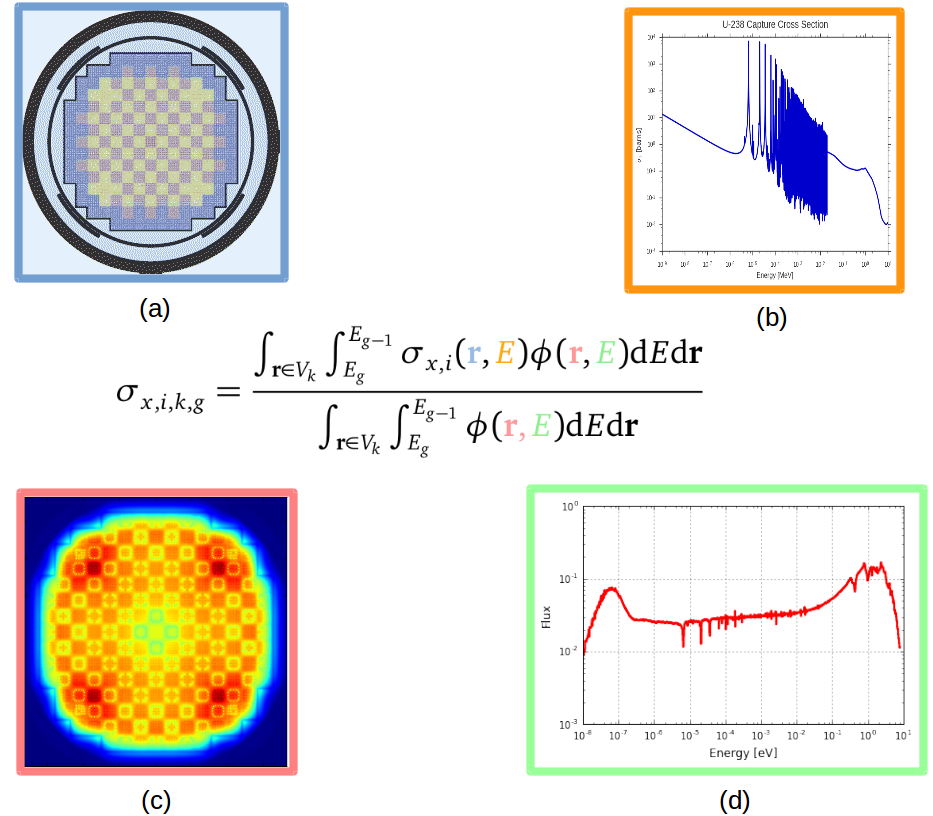
\includegraphics[width=0.9\linewidth]{figures/mgxs/mgxs-overlay}
\caption[Energy and spatial variation in \ac{MGXS}]{The calculation of multi-group cross sections requires knowledge of the spatial and energy variation of the continuous energy cross section and flux. The color-coded position $\mathbf{r}$ and energy $E$ variables correspond to the figures with the matching colored outlines. The microscopic cross section $\sigma_{x,i}$ depends on reactor configuration (a) and neutron energy (b). The flux $\phi$ varies with position (c) and energy (d).}
\label{fig:chap2-mgxs-overlay}
\end{figure}

The \ac{MGXS} are needed to compute the flux, but the flux is needed to compute \ac{MGXS}. As a result, an informed guess is generally made about the flux distribution in order to compute \ac{MGXS}. Such estimates of the flux introduce further approximations in addition to those presented in Secs.~\Crefrange{sec:chap2-approx-angle}{sec:chap2-approx-space}. The following section discusses a high-level overview of the standard multi-level approach to estimating the flux for \ac{MGXS} generation.

%An iterative approach could be used to resolve this issue, but the computational expense would prohibit such a scheme for practical whole-core calculations.

%\begin{dmath}
%\label{eqn:chap2-sigt-mg-color}
%\sigma_{x,i,k,g} = \frac{\int\displaylimits_{\mathbf{r} \in V_{k}} \int\displaylimits_{E_{g}}^{E_{g-1}} \sigma_{x,i}(\textcolor{carolinablue}{\mathbf{r}},\textcolor{darktangerine}{E})\phi(\textcolor{lightsalmonpink}{\mathbf{r}},\textcolor{lightgreen}{E})\mathrm{d}E\mathrm{d}\mathbf{r}}{\int\displaylimits_{\mathbf{r} \in V_{k}} \int\displaylimits_{E_{g}}^{E_{g-1}} \phi(\textcolor{lightsalmonpink}{\mathbf{r},\textcolor{lightgreen}{E}})\mathrm{d}E\mathrm{d}\mathbf{r}}
%\end{dmath}

%%%%%%%%%%%%%%%%%%%%%%%%%%%%%%
\subsection{Standard Multi-Level Approach}
\label{subsec:chap2-mgxs-lib-std-approach}

The standard techniques for multi-group cross section generation use a multi-level framework to draw a compromise between accuracy and computational efficiency. The goal in this process is to define a library of \ac{MGXS} which enforces an equivalence between an accurate fine-mesh transport calculation and a corresponding computationally efficient coarse mesh transport or diffusion calculation. The angular, energy and spatial variation of the flux is treated with varying degrees of complexity at each level as illustrated in Fig.~\ref{fig:chap2-mgxs-process}. The process begins with a resonance self-shielding calculation that solves the slowing down problem with point-wise nuclear cross section data in a simple infinite medium, slab or pin cell geometry. The self-shielding calculation produces an \ac{MGXS} library with $\mathcal{O}(100)$ energy groups that is next used by a lattice physics calculation to capture spectral interactions within and between fuel pins in each unique fuel assembly. The lattice physics calculation performs spatial homogenization across each assembly and produces a condensed library with $\mathcal{O}(2-10)$ groups. This assembly-homogenized few group \ac{MGXS} library is finally used by a whole-core nodal diffusion calculation.

\begin{figure}[h!]
  \centering
  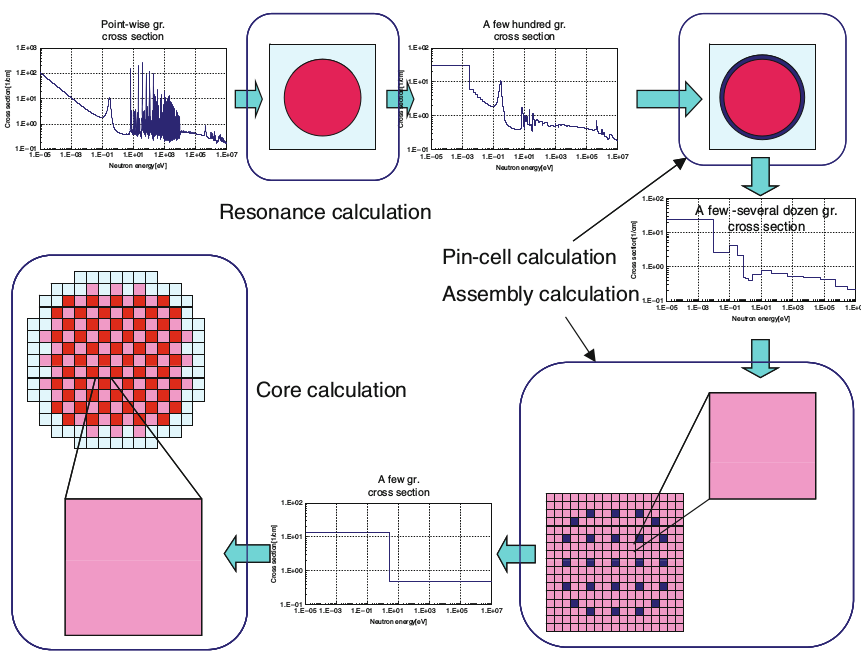
\includegraphics[width=0.9\linewidth]{figures/mgxs/nuke-handbook-mgxs-process}
\caption[Standard multi-level framework for MGXS generation]{The standard multi-level framework for \ac{MGXS} generation taken from the \textit{Handbook of Nuclear Engineering}~\cite{cacuci2010handbook}. The energy dependence of the nuclear cross sections is successively coarsened with resonance self-shielding and lattice physics calculations to generate multi-group libraries for whole-core simulations.}
\label{fig:chap2-mgxs-process}
\end{figure}

%The primary challenge throughout this multi-level scheme is to incorporate effects from the resonances in the point-wise cross sections. The spectral interactions which must be accurately accounted for are often referred to as \textit{self-shielding effects} in energy and space. 

The primary challenge throughout this multi-level scheme is to incorporate spectral interactions known as \textit{self-shielding effects} in energy and space. \textit{Energy self-shielding} refers to the impact that resonance interactions may have on the shape of the flux in energy. For example, the sharp depressions in \ac{PWR} flux spectra at energies near the large U-238 thermal capture resonances is an example of energy self-shielding (see Fig.~\ref{fig:chap2-mgxs-overlay}d). These depressions must be accurately captured in the flux used to generate \ac{MGXS}. \textit{Spatial self-shielding} refers to the impact of the material properties in different spatial zones on the flux in other nearby zones. For example, the outer rim of an \ac{LWR} fuel pin shields the center of the pin from neutrons in certain energy groups due to reactions such as U-238 resonance absorption.

%An empty control rod guide tube filled with water, for example, will provide additional moderation and therefore soften the spectrum for nearby fuel pins in \ac{LWR}s, which must be incorporated into the \ac{MGXS} calculation.

There is a long history of approximations for the flux for \ac{MGXS} generation~\cite{cacuci2010handbook}. These include the narrow, wide and intermediate resonance (NR, WR, and IR) approximations used to model the flux in a resonance self-shielding calculation. Lattice physics calculations typically use equivalence in dilution or subgroup methods to model physics in heterogeneous geometries. These approximations are based on simplifying assumptions regarding the geometric configuration, resonance interference effects (mutually overlapping resonances) and temperature distributions\footnote{Although the temperature dependence of cross sections has been neglected thus far for brevity, it must be captured in \ac{MGXS} libraries in order to model Doppler broadening for reactivity coefficient calculations.}. Although ultra-fine methods may be used to compute reference solutions for comparison, they are typically too computationally expensive for routine use. 

As a result of the various approximations employed to model the flux spectrum, the conventional approach for \ac{MGXS} generation is subject to significant engineering prescriptions for different reactor designs.  For example, modifications must be made to lattice physics calculations which account for the impact of local spatial heterogeneities, such as fuel rods adjacent to burnable absorbers. Similarly, it is typical to use infinite boundary conditions (reflective, periodic, white) in resonance self-shielding and lattice physics calculations. This may lead to approximation error in whole-core calculations which must model the neutron leakage spectra with vacuum boundary conditions, as well as the flux at the interface between different adjacent assemblies and/or a reflector. As a result, adjustments must be made to the standard multi-level approach in order for the final whole-core calculation to accurately account for the effects of spatial heterogeneity.


%%%%%%%%%%%%%%%%%%%%%%%%
\subsection{An Alternative Pathway with Monte Carlo}
\label{subsec:chap2-mgxs-lib-mc}

The multi-level approach of approximations used to generate \ac{MGXS} is the ``Achilles heel'' of multi-group methods. The approximate flux used to compute \ac{MGXS}, along with other approximations inherent in multi-group calculations, require careful use of multi-group methods for reactor analysis. As a result, Monte Carlo must be used to generate reference solutions for benchmarking and verification analysis of multi-group methods. In recent years, there has been growing interest in the use of \ac{MC} in the \ac{MGXS} generation process\cite{leppanen2007serpent,fridman2011serpent,
leppanen2016overview,dorval2015diff,ilas2003monte,pounders2006stochastically,
pounders2009diffusion,pounders2015history,cho2009generation,yun2010monte,
yamamoto2012buckling,yamamoto2012diff,shim2008generation,park2010assembly,park2012generation,
herman2013improved,liuphysor2016,okumura2000validation,tohjoh2005application,
gast1981procedure,ondis2000rcp01,blomquist2002status,redmond1997multigroup,
van2006homogenized,hoogenboom2007generation,yoshioka2010multigroup, yoshioka2011multi,
cai2014condensation,nelson2014improved}. since it offers a potential pathway to use a stochastic approximation to the exact flux in \ac{MGXS} generation.

Continuous energy Monte Carlo is considered the ``gold standard'' for neutron transport calculations since it is reactor agnostic and samples over the entire phase space of angle, energy and position. \ac{MC} is not widely used in routine reactor analysis, however, since its computational expense renders it many orders of magnitude slower than deterministic multi-group methods. Some recent work in the community adopts a hybrid approach which combines the resonance self-shielding and lattice physics stages in a single \ac{MC} simulation. These schemes minimize the computational expense by modeling sub-components (\textit{e.g.}, fuel pins and assemblies) rather than a full reactor. Although the hybrid approach has the advantage of using the ``true'' flux sampled in \ac{MC} to generate \ac{MGXS}, special treatment must still be given to accommodate infinite boundary conditions and neutron leakage spectra.

The following chapter introduces stochastic integration with \ac{MC} and its specific application to compute \ac{MGXS}. In addition, the chapter reviews past and present efforts to generate \ac{MGXS} with \ac{MC} for neutron diffusion and transport codes.


\vfill
\begin{highlightsbox}[frametitle=Highlights]
\begin{itemize}
%  \item Nuclear reactor analysis simulation methods present tradeoffs between accuracy and speed.
%  \item Monte Carlo methods are ``truest'' to the physics, but too computationally expensive for practical whole-core simulation.
  \item Numerical methods approximate the angular, energy and spatial variables in the neutron transport equation to make it computationally tractable.
  \item Multi-group theory treats a neutron's energy with a finite set of discrete energy groups. Multi-group theory is valid if \ac{MGXS} are defined to preserve reaction rates in each energy group.
  \item Energy condensation and spatial homogenization are used to compute \ac{MGXS} in each energy group and spatial zone. \ac{MGXS} generation requires the neutron flux in energy and space to average the continuous energy cross sections.
  \item Standard \ac{MGXS} generation methods use a multi-level approach to approximate the neutron flux, accounting for self-shielding effects. Flux approximations are based on engineering prescriptions for specific reactor configurations and spectra and are not generalizable to new core designs.
  \item Monte Carlo is a promising approach for \ac{MGXS} generation since it accurately produces an unbiased estimate of the flux without approximation.
\end{itemize}
\end{highlightsbox}
\vfill
\chapter{MGXS Generation with Monte Carlo}
\label{chap:mgxs-mc}

In the preceding chapter it was observed that many approximations are made in multi-group theory and the generation of multi-group cross sections. Monte Carlo is an approach to replace some of the steps in the standard multi-level framework for \ac{MGXS} generation with a natural and reactor agnostic treatment of energy and spatial self-shielding. This chapter presents a brief overview of \ac{MC} tallies and statistics in Sec.~\ref{sec:chap3-mc-overview}, outlines the necessary computation needed to generate \ac{MGXS} with \ac{MC} in Sec.~\ref{sec:chap3-mgxs-gen}, and discusses past studies which applied \ac{MC} for \ac{MGXS} generation in Sec.~\ref{sec:chap3-lit-review}.

%and Sec.~\ref{sec:chap3-mgxs-gen} outlines the necessary computation needed to generate \ac{MGXS} with \ac{MC}. Sec.~\ref{sec:chap3-lit-review} discusses past work to apply \ac{MC} for \ac{MGXS} generation, while Sec.~\ref{sec:chap3-latent-variables} introduces a new approach based on a latent variable model for spatial self-shielding.


%%%%%%%%%%%%%%%%%%%%%%%%%%%%%%%%%%%%%%%%%%%%%%%%%%%%%%%%%%%%%%%%%%%%%%%%%%%%%%%
\section{Overview of Monte Carlo Methods}
\label{sec:chap3-mc-overview}

Monte Carlo methods have been successfully applied to neutron transport calculations for many decades. A detailed accounting of the physics models and algorithms used in \ac{MC} methods can be found in the manuals for the Serpent~\cite{serpent2013manual}, MCNP~\cite{mcnpx2003manual}, and OpenMC~\cite{openmc2016manual} Monte Carlo particle transport codes. This section presents a few key aspects related to tallies and statistics, and follows directly from the manual for the OpenMC~\cite{openmc2016manual} code which is used throughout this work.

%%%%%%%%%%%%%%%%%%%%%%%%%%%%%%%%
\subsection{Monte Carlo Tallies}
\label{subsec:chap3-mc-tallies}

\ac{MC} simulations sample the particle distribution in order to compute integral quantities of interest called \textit{tallies}. A tally is an integral of a \textit{scoring function} $f$ weighted by the neutron distribution, or flux, across some region of phase space. A general form for tally $\mathcal{T}$ is given by the following integral expression:

\begin{dmath}
\label{eqn:chap3-tallies-general}
\mathcal{T} = \int_{V} \int_{S} \int_{E}  f(\mathbf{r},\mathbf{\Omega},E)\psi(\mathbf{r},\mathbf{\Omega},E)\mathrm{d}E\mathrm{d}\mathbf{\Omega}\mathrm{d}\mathbf{r} 
\end{dmath}

In OpenMC parlance, the integration bounds over space, angle and energy are termed \textit{filters}, while the scoring function $f$ is simply known as a \textit{score}. Various scores may be used to compute volume-integrated fluxes, reaction rates and functional expansions. \ac{MC} does not perform the integration in Eqn.~\ref{eqn:chap3-tallies-general} with the exact flux specified at all points in phase space. Instead, \ac{MC} performs stochastic integration by sampling the particle population across the entirety of phase space to compute a \textit{statistical estimate} $\hat{\mathcal{T}}$ of the true integral $\mathcal{T}$.

There are a number of different techniques to estimate a tally. The first and most general method is known as an \textit{analog estimator}. An analog estimator $\hat{\mathcal{T}}$ increments a tally by the particle weight $w_{i}$ each time an event $i$ occurs from the set of all events of interest $A$ (\textit{e.g.}, fission events). The sum of particle weights is then normalized by the total weight of all particles $W$ to compute the interaction frequency on a per-particle basis within the phase space volume of interest:

\begin{dmath}
\label{eqn:chap3-tallies-analog}
\hat{\mathcal{T}} = \frac{1}{W}\displaystyle\sum\limits_{i \in A} w_{i}
\end{dmath}

Although analog estimators permit general filters and scoring functions, they may suffer from poor tallying efficiency if the size of set $A$ is very small compared to the total number of events in a simulation. A \textit{collision estimator} improves the tallying efficiency by incrementing a tally more frequently than is possible with analog estimators. In particular, a collision estimator increments a tally at each collision $i$ from the set of all collisions $C$ irregardless of the types of collisions that took place. By noting that the total collision rate is given by $R_{t} = \Sigma_{t}\phi$, a collision estimator for the flux $\hat{\phi}$ may be simply defined by dividing the particle weights by the total macroscopic cross section:

\begin{dmath}
\label{eqn:chap3-tallies-collision-flux}
\hat{\phi} = \frac{1}{W}\displaystyle\sum\limits_{i \in C}\frac{w_{i}}{\Sigma_{t}(E_{i})}
\end{dmath}

\noindent The collision estimator depends on the energy of the incoming particle $E_{i}$ in order to scale the particle weight by the energy-dependent total cross section. It follows that the collision estimator for a reaction rate $\hat{\mathcal{R}}_{x}$ is the product of the flux in Eqn.~\ref{eqn:chap3-tallies-collision-flux} and the cross section for the reaction type $x$ of interest:

\begin{dmath}
\label{eqn:chap3-tallies-collision-rxn}
\hat{\mathcal{R}}_{x} = \frac{1}{W}\displaystyle\sum\limits_{i \in C}\frac{w_{i}\Sigma_{x}(E_{i})}{\Sigma_{t}(E_{i})}
\end{dmath}

The collision estimator increases the number of events in $C$ to improve the tallying efficiency with respect to analog tallies. A third method known as \textit{track-length estimators} goes one step further and increments a tally each time a particle trajectory crosses the phase space of interest (\textit{e.g.}, a spatial tally mesh zone) even if a collision did not take place. The track-length estimator makes use of a particle's distance traveled $\Delta\mathbf{r}$ to estimate the flux. A track-length estimator of the flux is therefore:

\begin{dmath}
\label{eqn:chap3-tallies-track-length-flux}
  \hat{\phi} = \frac{1}{W}\displaystyle\sum\limits_{i \in T}w_{i}\Delta\mathbf{r}_{i}
\end{dmath}

\noindent where the set $T$ represents each particle trajectory through the phase space volume of interest. Similarly, a track-length estimate of a reaction rate $x$ can be found by simply multiplying the flux in Eqn.~\ref{eqn:chap3-tallies-track-length-flux} by the cross section:

\begin{dmath}
\label{eqn:chap3-tallies-track-length-rxn}
  \hat{\mathcal{R}}_{x} = \frac{1}{W}\displaystyle\sum\limits_{i \in T}w_{i}\Delta\mathbf{r}_{i}\Sigma_{x}(E_{i})
\end{dmath}

The tallying efficiency for track-length estimators is greatly improved by incrementing a tally for each particle trajectory. As a result, the confidence intervals are generally much tighter for track-length estimators than those for analog and collision estimators. 

Each of the three estimators -- analog, collision and track-length -- may be useful for different scenarios. Although track-length and collision estimators improve statistics over analog estimates, they cannot be employed for all types of filters. For example, track-length tallies may not be used if the scoring function requires information about the outgoing particle since this is not available unless a collision took place. As discussed in Sec.~\ref{sec:chap3-mgxs-gen}, a mixture of estimators which tradeoff generality with efficiency must be used to generate \ac{MGXS} from \ac{MC} tallies.


%%%%%%%%%%%%%%%%%%%%%%%%%%%%%%
\subsection{Sample Statistics}
\label{subsec:chap3-mc-stats}

As discussed in the preceding section, \ac{MC} performs stochastic integration with one of a number of different estimators. In each case, the tally estimator $\hat{\mathcal{T}}$ is computed as a sample mean of of all of the events or particle trajectories simulated. An unbiased estimate of the sample mean is given by:

\begin{equation}
\label{eqn:chap3-sample-mean}
\bar{x} = \frac{1}{N} \displaystyle\sum\limits_{i=1}^{N} x_{i}
\end{equation}

\noindent where each of the $N$ samples is given by a random variable $x_{i}$. For \ac{MC} codes that use batch-based statistics, such as OpenMC, $N$ is the number of batches of particles simulated and $x_{i}$ is the tally estimator for the $i$\textsuperscript{th} batch of particles. 

Each of the random variables $x_{i}$ is sampled from some probability distribution representative of the physics in the simulation. The sampling distribution is normal such that $x_{i} \sim \mathcal{N}(\mu,\sigma^{2})$ where $\mathcal{N}(\mu,\sigma^{2})$ signifies a normal distribution with mean $\mu$ and variance $\sigma^{2}$ if each batch of particles is independent. An unbiased estimate of the variance $\sigma^{2}$ of the normal distribution from which the population $x_{i}$ is drawn may be estimated using Bessel's correction for the sample variance $s^{2}$:

\begin{equation}
\label{eqn:chap3-variance-sample}
s^{2} = \frac{1}{N-1}\displaystyle\sum\limits_{i=1}^{N}\left(x_{i} - \bar{x}\right)^{2}
\end{equation}

\noindent As $N \rightarrow \infty$ the population variance estimator will approach the true variance $\sigma^{2}$ of the underlying distribution. In the case of batch-based statistics, the variance $\sigma^{2}$ will be determined by the number of particles simulated per batch -- the more particle histories simulated per batch, the smaller $\sigma^{2}$ will be, and vice versa.

In general, it is more useful to quantify the uncertainty of a tally estimator than it is to compute the sample variance. The variance of the sample mean is representative of the distribution from which the random variable $\bar{x}$ is drawn and indicates the degree of confidence one may have in a tally estimator. By the Central Limit Theorem, the sample mean $\bar{x}$ will converge to the mean of a normal distribution if the samples $x_{i}$ are uncorrelated. An unbiased estimate of the variance of the sample mean can be derived from the Bienaym\'{e} formula to give:

\begin{equation}
\label{eqn:chap3-variance-mean}
s_{\bar{x}}^{2} = \frac{1}{N-1}\left(\frac{1}{N}\displaystyle\sum\limits_{i=1}^{N}
x_{i}^{2} - \bar{x}^2\right)
\end{equation}

A key observation is that the standard deviation of the sample mean is directly proportional to $\nicefrac{1}{\sqrt{N}}$ if the samples $x_{i}$ are uncorrelated. This necessarily implies that the uncertainties on a tally estimator can be made arbitrarily small given enough simulated particle histories. However, recent studies have shown that tally estimators in eigenvalue calculations are not generally independent and identically distributed realizations due to correlated fission sources between batches~\cite{herman2014correlation,miao2016correlation}. 

\begin{emphbox}
\textbf{Monte Carlo provides statistical estimators for quantities such as energy- and volume-integrated reaction rates and fluxes. Track-length estimators are more statistically efficient than analog and collision estimators, but are not generally applicable for scoring functions dependent on outgoing neutron energy.}
\end{emphbox}


%%%%%%%%%%%%%%%%%%%%%%%%%%%%%%%%%%%%%%%%%%%%%%%%%%%%%%%%%%%%%%%%%%%%%%%%%%%%%%%
\section{MGXS Generation with Monte Carlo}
\label{sec:chap3-mgxs-gen}

This section describes how multi-group cross sections may be computed using stochastic integration. Sec.~\ref{subsec:chap3-tally-types} outlines the types of OpenMC tallies needed to generate \ac{MGXS} -- including the scores, filters and estimators for each tally -- and the arithmetic combinations used to combine different tallies. Sec.~\ref{subsec:chap3-uncertainty-prop} illustrates how the uncertainties of the \ac{MGXS} may be estimated using error propagation theory.


%%%%%%%%%%%%%%%%%%%%%%%%
\subsection{Tally Types Needed for MGXS Generation}
\label{subsec:chap3-tally-types}

The types of \ac{MGXS} needed to solve the neutron transport equation were outlined in Chap.~\ref{chap:mgxs}, including expressions for the transport-corrected total cross section and scattering matrix, and the fission production cross section and emission spectrum. This section outlines the types of tallies needed to compute these \ac{MGXS}. It is important to note that the flux separability approximation (Sec.~\ref{subsec:chap2-angle}) is applied in the tally formulations for each of the group constants.

\subsubsection{Inner Product Notation}
\label{subsec:chap3-tally-types-notation}

The following sections use angle bracket notation $\langle \cdot , \cdot \rangle$ to represent inner products in phase space. This may correspond to integrals over incoming and/or outgoing energy, space, and angle. Using this notation, a tally estimator for reaction rate $x$ is represented as follows: 

\begin{equation}
\label{eqn:chap3-inner-prod-notation}
\langle \Sigma_x, \psi \rangle = \int_{V} \int_{S} \int_{E} \Sigma_{x}(\mathbf{r},E)\psi(\mathbf{r},E,\mathbf{\Omega}) \mathrm{d}E\mathrm{d}\mathbf{\Omega}\mathrm{d}\mathbf{r}
\end{equation}

\noindent This notation is specialized throughout this section with subscripts to indicate the subsets of phase space that are integrated over in the inner product. In particular, subscript $k$ refers to a volume integral over $V_{k}$ for some region of space $k$ for spatial homogenization (Sec.~\ref{subsec:chap2-space}), while subscript $g$ corresponds to an integral over energies with $E \in [E_{g}, E_{g-1}]$ for energy condensation (Sec.~\ref{subsec:chap2-energy}). For example, the microscopic reaction rate for reaction $x$ by nuclide $i$ is denoted as:

\begin{equation}
\label{eqn:chap3-angle-rxn-rate}
\langle \sigma_{x,i}, \psi \rangle_{k,g} = \int_{\mathbf{r} \in V_{k}} \int_{4\pi} \int_{E_{g}}^{E_{g-1}} \sigma_{x,i}(\mathbf{r},E)\psi(\mathbf{r},E,\mathbf{\Omega}) \mathrm{d}E\mathrm{d}\mathbf{\Omega}\mathrm{d}\mathbf{r}
\end{equation}

\noindent The inner product of a function with unity, such as the spatially-homogenized and energy-integrated flux is denoted by:

\begin{equation}
\label{eqn:chap3-angle-flux}
\langle \psi \rangle_{k,g} \equiv \langle \psi, \mathbb{1} \rangle_{k,g} = \int_{\mathbf{r} \in V_{k}} \int_{4\pi} \int_{E_{g}}^{E_{g-1}} \psi(\mathbf{r},E,\mathbf{\Omega}) \mathrm{d}E\mathrm{d}\mathbf{\Omega}\mathrm{d}\mathbf{r}
\end{equation}

Finally, the superscripts $a$ and $t\ell$ are given to those inner products computed with analog and track-length estimators, respectively -- \textit{i.e.}, $\langle \cdot,\cdot \rangle^{a}$ is an analog tally estimator and $\langle \cdot,\cdot \rangle^{t\ell}$ is a track-length tally estimator of the corresponding inner products.


\subsubsection{General Reaction Cross Section}
\label{subsubsec:chap3-gen-xs}

A general spatially-homogenized and energy condensed macroscopic multi-group cross section for reaction $x$, spatial zone $k$, energy group $g$ can be computed with track-length tally estimators in OpenMC. The \ac{MGXS} is simply the ratio of the group-wise reaction rates $\langle \Sigma_{x}, \psi \rangle_{k,g}^{t\ell}$ and fluxes $\langle \psi \rangle_{k,g}^{t\ell}$:

\begin{equation}
\label{eqn:chap3-general-macro}
\hat{\Sigma}_{x,k,g} = \frac{\langle \Sigma_{x}, \psi \rangle_{k,g}^{t\ell}}{\langle \psi \rangle_{k,g}^{t\ell}}
\end{equation}

\noindent Likewise, a microscopic \ac{MGXS} for nuclide $i$ can be computed as follows:

\begin{equation}
\label{eqn:chap3-general-micro}
\hat{\sigma}_{x,i,k,g} = \frac{\langle \sigma_{x,i}, \psi \rangle_{k,g}^{t\ell}}{\langle \psi \rangle_{k,g}^{t\ell}}
\end{equation}

These estimators are used for reaction types which are only dependent on the incoming energy of a neutron, such as total and radiative capture reactions.


\subsubsection{Total Cross Section}
\label{subsubsec:chap3-tally-types-tot-xs}

The total macroscopic cross section $\Sigma_{t}$ is a special case of Eqn.~\ref{eqn:chap3-general-micro}, with track-length estimators for the total collision rate and flux:

\begin{equation}
\label{eqn:chap3-total-macro}
\hat{\Sigma}_{t,k,g} = \frac{\langle \Sigma_{t}, \psi \rangle_{k,g}^{t\ell}}{\langle \psi \rangle_{k,g}^{t\ell}}
\end{equation}

As discussed in Sec.~\ref{subsec:chap2-transport-corr}, a transport correction is often used to incorporate anisotropic scattering effects into the transport equation with an isotropic scattering kernel. An expression for the in-scatter approximation~\cite{yamamoto2008simplified} to the transport correction can be computed with an OpenMC tally for the first Legendre scattering moment\footnote{It is assumed that scattering multiplicity is included in the scattering moments as discussed in Sec.~\ref{sec:chap2-scatt-prod}.}. The inner product for this tally is given by:

\begin{equation}
\label{eqn:chap3-sigs1}
\langle \Sigma_{s1}, \psi \rangle_{k,g'\rightarrow g} = \int_{\mathbf{r} \in V_{k}} \int_{4\pi} \int_{E_{g}}^{E_{g-1}} \int_{E_{g'}}^{E_{g'-1}} \Sigma_{s1}(\mathbf{r},E'\rightarrow E)\psi(\mathbf{r},E',\mathbf{\Omega}) \mathrm{d}E'\mathrm{d}E\mathrm{d}\mathbf{\Omega}\mathrm{d}\mathbf{r}
\end{equation}

\noindent An analog estimator must be used in OpenMC since the tally includes an integral over the outgoing neutron energy. The spatially-homogenized and energy condensed transport-corrected total cross section given in Eqn.~\ref{eqn:chap2-transport-xs} is computed by summing over all incoming energy groups:

\begin{equation}
\label{eqn:chap3-transport-corr-macro}
\Delta\hat{\Sigma}_{tr,k,g} = \displaystyle\sum\limits_{g'=1}^{G} \langle{\Sigma_{s1}, \psi \rangle_{k,g'\rightarrow g}^{a}}
\end{equation}

\noindent The transport correction is then subtracted from the group-wise total collision rate and normalized by the flux to compute the transport-corrected total cross section:

\begin{equation}
\label{eqn:chap3-sigt-transport-macro}
\hat{\tilde{\Sigma}}_{t,k,g} = \frac{\langle \Sigma_{t}, \psi \rangle_{k,g}^{a} - \Delta\hat{\Sigma}_{tr,k,g}}{\langle \psi \rangle_{k,g}^{a}}
\end{equation}

\noindent Note that since the transport correction must be computed using an analog estimator, the total collision and flux in Eqn.~\ref{eqn:chap3-sigt-transport-macro} must also be computed with analog estimators.


\subsubsection{Scattering Matrix}
\label{subsubsec:chap3-tally-types-scatt-mat}

The isotropic scattering matrix is computed with an inner product of scattering reactions over both incoming and outgoing energies. An analog estimator must be used since the integral is dependent on the neutron's outgoing energy. Similar to the first Legendre moment in Eqn.~\ref{eqn:chap3-sigs1}, the isotropic scattering moment is given by the following expression:

\begin{equation}
\label{eqn:chap3-sigs0}
\langle \Sigma_{s0}, \psi \rangle_{k,g'\rightarrow g} = \int_{\mathbf{r} \in V_{k}} \int_{4\pi} \int_{E_{g}}^{E_{g-1}} \int_{E_{g'}}^{E_{g'-1}} \Sigma_{s0}(\mathbf{r},E'\rightarrow E)\psi(\mathbf{r},E,\mathbf{\Omega}) \mathrm{d}E'\mathrm{d}E\mathrm{d}\mathbf{\Omega}\mathrm{d}\mathbf{r}
\end{equation}

\noindent The isotropic scattering matrix is then:

\begin{equation}
\label{eqn:chap3-scatter-macro}
\hat{\Sigma}_{s,k,g'\rightarrow g} = \frac{\langle \Sigma_{s0}, \psi \rangle_{k,g'\rightarrow g}^{a}}{\langle \psi \rangle_{k,g'}^{a}}
\end{equation}

\noindent The transport correction in Eqn.~\ref{eqn:chap3-transport-corr-macro} can be applied by subtracting it from the diagonal elements in the matrix to compute the transport-corrected scattering matrix:

\begin{equation}
\label{eqn:chap3-scatter-trans-macro}
\hat{\tilde{\Sigma}}_{s,k,g'\rightarrow g} = \frac{\langle \Sigma_{s0}, \psi \rangle_{k,g'\rightarrow g}^{a} - \delta_{g,g'} \Delta\hat{\Sigma}_{tr,k,g}}{\langle \psi \rangle_{k,g'}^{a}}
\end{equation}

%\begin{equation}
%\label{eqn:chap3-scatter-trans-macro}
%\hat{\tilde{\Sigma}}_{s,k,g'\rightarrow g} = \frac{\langle \Sigma_{s0}, \psi \rangle_{k,g'\rightarrow g}^{a} - \delta_{g,g'} \displaystyle\sum\limits_{g''=1}^{G} \langle{\Sigma_{s1}, \psi \rangle_{k,g''\rightarrow g}^{a}}}{\langle \psi \rangle_{k,g'}^{a}}
%\end{equation}


\subsubsection{Fission Production Cross Section}
\label{subsubsec:chap3-tally-types-fiss-prod}

The fission production cross section was condensed in Eqn.~\ref{eqn:chap2-nusifg} to make it independent of the energies of the neutrons emitted from fission. It is therefore straightforward to treat the fission product macroscopic cross section $\nu\Sigma_{f}$ as a special case of Eqn.~\ref{eqn:chap3-general-micro}, with track-length estimators for the total collision rate and flux:

\begin{equation}
\label{eqn:chap3-nu-fiss-macro}
\nu\hat{\Sigma}_{f,k,g} = \frac{\langle \nu\Sigma_{f}, \psi \rangle_{k,g}^{t\ell}}{\langle \psi \rangle_{k,g}^{t\ell}}
\end{equation}


\subsubsection{Fission Energy Spectrum}
\label{subsubsec:chap3-tally-types-chi}

Unlike the fission production cross section, the fission spectrum is dependent on the outgoing neutron energy and must be computed with analog estimators. The fission production matrix from group $g'$ into group $g$ is given by the following inner product:

\begin{equation}
\label{eqn:chap3-nu-fiss-energies}
\langle \nu\Sigma_{f}, \psi \rangle_{k,g'\rightarrow g} = \int_{\mathbf{r} \in V_{k}} \int_{4\pi} \int_{E_{g}}^{E_{g-1}} \int_{E_{g'}}^{E_{g'-1}} \nu\Sigma_{f}(\mathbf{r},E'\rightarrow E)\psi(\mathbf{r},E,\mathbf{\Omega}) \mathrm{d}E'\mathrm{d}E\mathrm{d}\mathbf{\Omega}\mathrm{d}\mathbf{r}
\end{equation}

\noindent The fission spectrum in Eqn.~\ref{eqn:chap2-nusifg} can then be computed from this tally by summing over incoming and outgoing energy groups:

\begin{equation}
\label{eqn:chap3-chi}
\hat{\chi}_{k,g} = \frac{\displaystyle\sum\limits_{g'=1}^{G} \langle \nu\Sigma_{f}, \psi \rangle_{k,g'\rightarrow g}^{a}}{\displaystyle\sum\limits_{g=1}^{G} \displaystyle\sum\limits_{g'=1}^{G} \langle \nu\Sigma_{f}, \psi \rangle_{k,g'\rightarrow g}^{a}}
\end{equation}

\noindent This expression for the fission spectrum will result in a normalized discrete probability distribution for the energy of neutrons emitted from fission.


\subsubsection{Summary}
\label{subsubsec:chap3-tally-types-summary}

The tallies needed to generate \ac{MGXS} libraries were outlined in detail in the preceding sections, and are summarized in Table~\ref{table:chap3-tally-types}. The scores and filters correspond to the notation used by the OpenMC code to describe the scoring function and integration bounds used in Eqn.~\ref{eqn:chap3-tallies-general}. 
The energy group structure for energy condensation is specified by \texttt{energy} and/or \texttt{energyout} filters in the table. The regions for spatial homogenization are specified by \texttt{material} or \texttt{cell} filters, although this could potentially include \texttt{universe}, \texttt{distribcell} and \texttt{mesh} filters as well.

%\renewcommand{\arraystretch}{1.5}

\begin{table}[h!]
  \centering
  \caption[Tally types for \ac{MGXS} generation]{The types of tallies used in \ac{MGXS} generation with OpenMC.}
  \scriptsize
  \label{table:chap3-tally-types}
  \vspace{6pt}
  \begin{tabular}{ m{1.3cm} m{1cm} m{2cm} m{2.5cm} m{2.5cm} m{1.5cm} }
  \toprule
  {\bf Name} &
  {\bf Symbol} &
  {\bf Tally} &
  {\bf Score} &
  {\bf Filters} &
  {\bf Estimator} \\

  \specialrule{.2em}{.1em}{.1em}

  \multirow{2}{*}[-0.7em]{\bf General} & \multirow{2}{*}[-0.7em]{$\hat{\Sigma}_{x,k,g}$} & $\langle \Sigma_{x}, \psi \rangle_{k,g}$ & reaction $x$ & \parbox{2cm}{\texttt{material}/\texttt{cell} \texttt{energy}} & \texttt{track-length} \\
  \cline{3-6}
  & & $\langle \psi \rangle_{k,g}$ & {\texttt{flux}} & \parbox{2cm}{\texttt{material}/\texttt{cell} \texttt{energy}} & \texttt{track-length} \\

  \specialrule{.2em}{.1em}{.1em}

  \multirow{2}{*}[-0.7em]{\bf Total} & \multirow{2}{*}[-0.7em]{$\hat{\Sigma}_{t,k,g}$} & $\langle \Sigma_{t}, \psi \rangle_{k,g}$ & \texttt{total} & \parbox{2cm}{\texttt{material}/\texttt{cell} \texttt{energy}} & \texttt{track-length} \\
  \cline{3-6}
  & & $\langle \psi \rangle_{k,g}$ & \texttt{flux} & \parbox{2cm}{\texttt{material}/\texttt{cell} \texttt{energy}} & \texttt{track-length} \\

  \specialrule{.2em}{.1em}{.1em}

  \multirow{3}{*}[-1em]{\parbox{1.5cm}{\bf Transport-Corrected Total}} & \multirow{3}{*}[-1em]{$\hat{\tilde{\Sigma}}_{t,k,g}$} & $\langle \Sigma_{t}, \psi \rangle_{k,g}$ & \texttt{total} & \parbox{2cm}{\texttt{material}/\texttt{cell} \texttt{energy}} & \texttt{analog} \\
  \cline{3-6}
  & & $\langle \Sigma_{s1}, \psi \rangle_{k,g'\rightarrow g}$ & \texttt{nu-scatter-1} & \parbox{2cm}{\texttt{material}/\texttt{cell} \texttt{energyout}} & \texttt{analog} \\
  \cline{3-6}
  & & $\langle \psi \rangle_{k,g}$ & \texttt{flux} & \parbox{2cm}{ \texttt{material}/\texttt{cell} \texttt{energy}} & \texttt{analog} \\

  \specialrule{.2em}{.1em}{.1em}

  \multirow{2}{*}[-0.5em]{\parbox{1.5cm}{\bf Scattering Matrix}} & \multirow{2}{*}[-0.5em]{$\hat{\Sigma}_{s,k,g'\rightarrow g}$} & $\langle \Sigma_{s0}, \psi \rangle_{k,g'\rightarrow g}$ & \texttt{nu-scatter-0} & \parbox{2cm}{\texttt{material}/\texttt{cell} \texttt{energy} \texttt{energyout}} & \texttt{analog} \\
  \cline{3-6}
  & & $\langle \psi \rangle_{k,g}$ & \texttt{flux} & \parbox{2cm}{\texttt{material}/\texttt{cell} \texttt{energy}} & \texttt{analog} \\

  \specialrule{.2em}{.2em}{.2em}

  \multirow{3}{*}[-1em]{\parbox{1.5cm}{\bf Transport-Corrected Scattering Matrix}} & \multirow{3}{*}[-1em]{$\hat{\tilde{\Sigma}}_{s,k,g'\rightarrow g}$} & $\langle \Sigma_{s0}, \psi \rangle_{k,g'\rightarrow g}$ & \texttt{nu-scatter-0} & \parbox{2cm}{\texttt{material}/\texttt{cell} \texttt{energy} \texttt{energyout}} & \texttt{analog} \\
  \cline{3-6}
  & & $\langle \Sigma_{s1}, \psi \rangle_{k,g'\rightarrow g}$ & \texttt{nu-scatter-1} & \parbox{2cm}{\texttt{material}/\texttt{cell} \texttt{energyout}} & \texttt{analog} \\
  \cline{3-6}
  & & $\langle \psi \rangle_{k,g}$ & \texttt{flux} & \parbox{2cm}{\texttt{material}/\texttt{cell} \texttt{energy}} & \texttt{analog} \\

  \specialrule{.2em}{.1em}{.1em}

  \multirow{2}{*}[-0.5em]{\parbox{1.5cm}{\bf Fission \hspace{1cm} Production}} & \multirow{2}{*}[-0.5em]{$\nu\hat{\Sigma}_{f,k,g}$} & $\langle \nu\Sigma_{f}, \psi \rangle_{k,g}$ & \texttt{nu-fission} & \parbox{2cm}{\texttt{material}/\texttt{cell} \texttt{energy}} & \texttt{track-length} \\
  \cline{3-6}
  & & $\langle \psi \rangle_{k,g}$ & \texttt{flux} & \parbox{2cm}{\texttt{material}/\texttt{cell} \texttt{energy}} & \texttt{track-length} \\

  \specialrule{.2em}{.1em}{.1em}
  
  \parbox{1.5cm}{\bf Fission Spectrum} & $\hat{\chi}_{k,g}$ & $\langle \nu\Sigma_{f}, \psi \rangle_{k,g'\rightarrow g}$ & \texttt{nu-fission} & \parbox{2cm}{\texttt{material}/\texttt{cell} \texttt{energy} \texttt{energyout}} & \texttt{analog} \\
  \midrule

\end{tabular}
\end{table}


%%%%%%%%%%%%%%%%%%%%%%%%%%%%%%%%%%%%
\subsection{Uncertainty Propagation}
\label{subsec:chap3-uncertainty-prop}

As discussed in the preceding sections, \ac{MGXS} may be computed using arithmetic combinations of tally estimators for reaction rates and fluxes. Each tally estimator is a random variable with an associated uncertainty estimated by the variance of the sample mean in Eqn.~\ref{eqn:chap3-variance-mean}. As a result, each multi-group cross section computed for a spatial zone and energy group is itself a random variable from a distribution with some unknown variance. It is therefore useful to estimate the uncertainty of \ac{MGXS} computed from \ac{MC} tallies in order to quantify whether the \ac{MGXS} are known with enough precision for accurate multi-group calculations. 

Estimates of the variance may be deduced from standard error propagation theory. Such analysis is widely discussed in the literature~\cite{bevington2003data}. A few key equations necessary to estimate the variance for \ac{MGXS} are reproduced here. The arithmetic combinations of interest for \ac{MGXS} generation include addition, subtraction, multiplication and division. 

Consider two random variables $X$ and $Y$, generated from distributions with variances $\sigma_{X}^2$ and $\sigma_{Y}^2$ which are arithmetically combined into a new random variable $Z$ with variance $\sigma_{Z}^2$. The random variables $X$ and $Y$ may correspond to tallies for reaction rates and the flux, while $Z$ could correspond to a \ac{MGXS}. The following expressions can be derived for the variance $\sigma_{Z}^{2}$ for binary combinations of $X$ and $Y$:

\vspace{-0.4in}

\begin{align*}
Z &= X + Y & \sigma_{Z}^{2} &= \sigma_{X}^{2} + \sigma_{Y}^{2} + 2\sigma_{XY} \numberthis \label{eqn:chap3-add} \\
Z &= X - Y & \sigma_{Z}^{2} &= \sigma_{X}^{2} + \sigma_{Y}^{2} - 2\sigma_{XY} \numberthis \label{eqn:chap3-sub} \\
Z &= XY & \sigma_{Z}^{2} &\approx Z^{2}\left[\left(\frac{\sigma_{X}}{X}\right)^{2} + \left(\frac{\sigma_{Y}}{Y}\right)^{2} + 2\frac{\sigma_{XY}}{Z}\right] \numberthis \label{eqn:chap3-mult} \\
Z &= \frac{X}{Y} & \sigma_{Z}^{2} &\approx Z^{2}\left[\left(\frac{\sigma_{X}}{X}\right)^{2} + \left(\frac{\sigma_{Y}}{Y}\right)^{2} - 2\frac{\sigma_{XY}}{Z}\right] \numberthis \label{eqn:chap3-div} \\
\end{align*}

\vspace{-0.4in}

\noindent These expressions are given in terms of the covariance $\sigma_{XY}$ of $X$ and $Y$:

\vspace{-0.1in}

\begin{equation}
\label{eqn:chap3-covariance}
\sigma_{XY} = \mathbb{E}[(X - \mathbb{E}[X])(Y - \mathbb{E}[Y])]
\end{equation}

\noindent where $\mathbb{E}[\cdot]$ is the expectation operator. The covariance is not generally computable using the standard formulation for a tally estimator in a Monte Carlo simulation. Although it would be possible to estimate the covariance using ensemble statistics\footnote{The covariance could be estimated from the results of an ensemble of independent \ac{MC} simulations.}, this is not often feasible. Instead, the covariance terms in Eqns.~\Crefrange{eqn:chap3-add}{eqn:chap3-div} are typically neglected. In general, the random variables for reaction rates and fluxes in the same volume of phase space are highly correlated, and neglecting the covariance leads to a poor approximation for the variance of \ac{MGXS}. However, it should be noted that division is the primary operation needed to combine tallies to compute \ac{MGXS}. Since the reaction rates and flux tallies must be positively correlated, the covariance term in Eqn.~\ref{eqn:chap3-div} reduces the estimate of the covariance. It therefore follows that a conservative estimate of the variance for \ac{MGXS} is obtained by neglecting the covariance.

\begin{emphbox}
\textbf{A mixture of analog and track-length \ac{MC} tallies for reaction rates and fluxes are used to generate spatially-homogenized and energy condensed \ac{MGXS}. Error propagation theory is used to estimate the \ac{MGXS} uncertainties.}
\end{emphbox}


%%%%%%%%%%%%%%%%%%%%%%%%%%%%%%%%%%%%%%%%%%%%%%%%%%%%%%%%%%%%%%%%%%%%%%%%%%%%%%%
\section{A Literature Review of MGXS Generation with MC}
\label{sec:chap3-lit-review}

The last two decades have seen growing interest in Monte Carlo as a means to generate \ac{MGXS} libraries. This section presents a brief overview of the literature which document these efforts. As discussed in Sec.~\ref{subsec:chap3-lit-review-diffusion}, most of the work to date has been directed at generating homogenized few-group constants for coarse mesh diffusion-based codes. Sec.~\ref{subsec:chap3-lit-review-transport} reviews a few recent theses which develop \ac{MC}-based methods to generate \ac{MGXS} for fine-mesh transport-based simulations, which is the motivation for this thesis.


\subsection{MGXS for Coarse Mesh Diffusion Calculations}
\label{subsec:chap3-lit-review-diffusion}

Most \ac{MC}-based \ac{MGXS} generation schemes to date focus on generating few-group constants for coarse mesh diffusion codes\footnote{In this context, \textit{coarse mesh} refers to the use of one or a few homogenized mesh cells per assembly.}. These schemes aim to improve the accuracy of standard diffusion codes for analysis of atypical core configurations for which the simplifications made by multi-level deterministic \ac{MGXS} generation methods are not necessarily applicable. These efforts replace the separate resonance self-shielding and deterministic lattice physics calculation steps in multi-level approaches (see Sec.~\ref{subsec:chap2-mgxs-lib-std-approach}) with fully-detailed \ac{MC} calculations of each assembly to compute the few-group constants needed by whole core diffusion codes. The widely used Serpent code discussed in Sec.~\ref{subsec:chap3-lit-review-diffusion-serpent} has led this trend over the last decade, and a few authors have applied the MCNP and McCARD codes in a similar fashion as highlighted in Secs.~\ref{subsec:chap3-lit-review-diffusion-mcnp} and \ref{subsec:chap3-lit-review-diffusion-mccard}. The latter subsections summarize studies which used the MC21, MVP-BURN, RCP01 and VIM codes to generate \ac{MGXS} for coarse mesh diffusion calculations.

\subsubsection{Serpent}
\label{subsec:chap3-lit-review-diffusion-serpent}

Serpent is a continuous energy Monte Carlo code developed by the VTT Technical Research Centre of Finland, and is one of the most widely used \ac{MC} particle transport codes in the world~\cite{serpent2013manual}. Serpent was initially created as part of Lepp{\"a}nen's thesis~\cite{leppanen2007serpent} to generate few-group constants for nodal diffusion codes. More recently, Serpent has developed into a general purpose reactor physics burnup code with features including isotopic depletion, on-the-fly Doppler broadening and support for CAD geometries.

Serpent is designed to be a drop-in replacement for deterministic resonance self-shielding and lattice physics calculation codes and can generate homogenized few-group constants for coarse mesh sub-assembly geometries. Serpent is uniquely designed for coarse mesh \ac{MGXS} generation since it uses the Woodcock-Delta method~\cite{woodcock1965techniques} to greatly reduce the computational expense of tracking particles in geometries with complicated surface crossings. Unlike deterministic multi-level approaches, Serpent uses \ac{MC} to precisely model self-shielding effects in complicated geometries. In addition, Serpent simplifies the validation of downstream diffusion codes which use the \ac{MGXS} it generates since it is also capable of computing whole-core reference solutions.

One of the challenges for lattice physics calculations is the appropriate treatment of net current between assemblies. In order to address this, Serpent employs a two-step energy condensation scheme including an infinite lattice calculation followed by a B$_{1}$ leakage correction~\cite{fridman2011serpent}. The scheme first performs an infinite lattice calculation for each unique assembly and tallies \ac{MGXS} in the WIMS 69-group structure. The \ac{MGXS} are used to form the B$_{1}$ equations for the homogenized system which are solved for the critical flux spectrum accounting for inter-assembly leakage. The critical flux is finally used to collapse the 69-group \ac{MGXS} into few-group constants. Although the B$_{1}$ equations make assumptions that are not always true -- such as an energy-independent buckling -- the approach has been demonstrated to largely resolve 20\% errors in 2-group diffusion coefficients compared to those collapsed with the infinite flux for simple \ac{PWR} benchmarks~\cite{fridman2011serpent}. However, the B$_{1}$ leakage correction does have some known deficiencies, including its inability to treat non-fissile regions such as homogenized reflectors or transmutation cross sections in burnup calculations~\cite{leppanen2016overview}.

Much of the research focus for Serpent has revolved around the need to accurately compute diffusion coefficients. Unlike the total, scattering, and fission production \ac{MGXS} discussed in Chap.~\ref{chap:mgxs}, diffusion coefficients do not have a continuous energy counterpart in transport theory. Serpent uses an approximate method to compute the Selengut-Goertzel diffusion coefficient from the inverse of the transport cross section\footnote{This is an approximate method since the energy collapse of the transport cross section is not equivalent to the energy collapse of its inverse, which is what is needed to collapse the diffusion coefficient.}. In particular, Serpent tallies a 69-group \ac{MGXS} transport cross section, and condenses its inverse with the B$_{1}$ leakage corrected spectra to compute diffusion coefficients. In addition, since it is not straightforward to compute current-weighted tallies in \ac{MC}, Serpent makes a heuristic approximation and uses a scalar flux-weighted scattering moment to compute the transport cross section (see Sec.~\ref{subsec:chap2-transport-corr}). More recently, the Serpent team has investigated a novel current-weighted scheme for directional diffusion coefficients~\cite{dorval2015diff}, and introduced Liu's novel Cumulative Migration Method (CMM)~\cite{liuphysor2016} to mitigate shortcomings in the current approach~\cite{leppanen2016overview}.

Although Serpent is the most popular tool for \ac{MGXS} generation, its use thus far has been specifically focused on coarse mesh diffusion applications. To the author's knowledge, there have not yet been any published works which use Serpent to generate \ac{MGXS} for fine-mesh transport calculations.

%In addition, as discussed in Sec.~\ref{subsec:chap2-transport-corr}, it is not is not a straighforward exercise to compute the transport cross section from Monte Carlo since it requires a first order current-weighted scattering moment matrix. Instead, Serpent makes a heuristic approximation and uses a scalar flux-weighted scattering moment to compute the transport cross section. 

\subsubsection{MCNP}
\label{subsec:chap3-lit-review-diffusion-mcnp}

The widely used MCNP code~\cite{mcnpx2003manual} developed by Los Alamos National Laboratory has also been employed to generate few-group \ac{MGXS} for coarse mesh diffusion methods. Perhaps the most comprehensive study can be found in Pounder's thesis~\cite{pounders2006stochastically} which, like Serpent, aimed to improve the accuracy of standard diffusion codes by generating improved diffusion coefficients with Monte Carlo. In addition to the reactor problems considered in Pounders' thesis, MCNP has also been used to generate diffusion coefficients for analysis of spent fuel storage lattices~\cite{ilas2003monte}.

Pounders considered several approaches to compute diffusion coefficients with Monte Carlo and implemented each in MCNP. The simplest method computed the diffusion coefficient as the inverse of the transport cross section. This formulation is most similar to that used in Serpent, but did not include a fine-to-few-group collapse with the B$_{1}$ leakage corrected spectra. Pounders also considered the flux-limited diffusion coefficient~\cite{pomraning1984flux} widely used in radiation hydrodynamics codes. In addition, Pounders developed an approach to use directional neutron currents to appropriately weight the first order scattering moment needed to compute the transport cross section. Lastly, Pounders' most novel contribution, termed the ``stochastic diffusion coefficient,'' attempted to embed higher order anisotropies in the diffusion coefficient by combining direction-dependent diffusion coefficients with volume-integrated flux gradient tallies.

Pounders' results demonstrated that the stochastic diffusion coefficient produced the best results since it mitigated the approximations imposed by P$1$ theory. However, the analysis was limited to simple 1D slab and 2D pin cell problems since the implementation of stochastic diffusion coefficients for arbitrary 3D reactor geometries would be challenging. Most interestingly, Pounders' thesis concluded that the error resulting from diffusion theory's assumption of a linearly anisotropic flux dominated the error induced by each of the diffusion coefficient formulations. Pounders thesis has served as the basis for the development of new methods to generate \ac{MGXS} with MCNP, including new diffusion coefficient formulations~\cite{pounders2009diffusion} and an approach to represent the Legendre expansion of the scattering kernel with equiprobable cosine bins~\cite{pounders2015history}.

A few recent studies have evaluated new leakage models for multi-group diffusion coefficient generation with MCNP. Yun and Cho evaluated a hybrid approach to compute diffusion coefficients with MCNP using an albedo-corrected leakage spectrum~\cite{cho2009generation,yun2010monte}. This approach iterated between a Monte Carlo lattice and deterministic whole-core calculations to converge nodal diffusion parameters to preserve surface currents to match a criterion defined by any arbitrary leakage model. Cho evaluated the method for a \ac{PWR} fuel assembly and demonstrated a slight improvement in the solution compared to a diffusion calculation with \ac{MGXS} weighted by an infinite spectrum.

Yamamoto~\cite{yamamoto2012buckling} developed a method to model neutron leakage with a correction term in the transport equation which is equivalent to the B$_{1}$ leakage correction method. The correction term was introduced in MCNP as a complex-valued particle weight in order to generate anisotropic diffusion coefficients~\cite{yamamoto2012diff}. Few-group diffusion coefficients for pin cell and assembly benchmarks exhibited good agreement with those generated by a reference deterministic code, but no criticality calculations were performed to validate eigenvalues and power distributions computed by a diffusion code.

\subsubsection{McCARD}
\label{subsec:chap3-lit-review-diffusion-mccard}

The McCARD Monte Carlo transport code developed by Seoul National University has been utilized in a number of studies to generate few-group constants for whole-core diffusion analysis~\cite{shim2008generation, park2010assembly, park2012generation}. The over-arching objective in these studies was to develop and evaluate a method to model the leakage spectrum in \ac{MC} lattice physics calculations. An approach was independently developed which used the solution to the homogeneous B$_{1}$ equations which is equivalent to the methodology used in the Serpent code~\cite{fridman2011serpent}. In summary, McCARD tallied fine group \ac{MGXS} and used the critical spectrum solved from the B$_{1}$ equations to collapse the fine group \ac{MGXS} into few-group constants. Like Serpent, McCARD uses the flux rather than the current to weight the first order scattering moment tallies to approximately compute fine group transport cross sections. The studies published in the literature validated the \ac{MGXS} generated with McCARD with a reference deterministic lattice code. In addition, good agreement was demonstrated between reference \ac{MC} and deterministic diffusion solutions for the eigenvalues and power distributions for 3D \ac{PWR} and gas-cooled, TRistructural-ISOtopic (TRISO) fueled Very High Temperature Reactor (VHTR) benchmark configurations. Finally, the B$_{1}$ leakage corrected spectra was shown to significantly improve the eigenvalue estimates and assembly-wise power distributions with respect to \ac{MGXS} computed from an infinite lattice spectrum.

\subsubsection{MC21}
\label{subsec:chap3-lit-review-diffusion-mc21}

Herman utilized the MC21 code developed by Knolls Atomic Power Laboratory to evaluate two approximations used in Monte Carlo calculations of diffusion coefficients~\cite{herman2013improved}. His work was motivated by approximations made by the multi-step energy condensation methodology used to compute diffusion coefficients in Serpent with a B$_{1}$ leakage corrected spectra. First, Herman considered whether to energy condense the fine group transport cross sections or diffusion coefficients when computing few-group diffusion coefficients. Second, he presented an approach to use a pre-tabulated form of the energy-dependent scattering cosine to correct the traditional form of the diffusion coefficient. His results demonstrated a significant reduction from more than 3\% to nearly 0.25\% in the reconstructed pin powers for a \ac{PWR} assembly. Herman's corrected diffusion coefficient was implemented in the OpenMC code~\cite{romano2013openmc} for use in \ac{CMFD} acceleration~\cite{herman2014monte}, and has inspired the development of the Cumulative Migration Method (CMM) to calculate diffusion coefficients with Monte Carlo~\cite{liuphysor2016}.

\subsubsection{MVP-BURN}
\label{subsec:chap3-lit-review-diffusion-mvp-burn}

Tohjoh used the MVP-BURN Monte Carlo code~\cite{okumura2000validation} to generate few-group constants for full core \ac{BWR} analysis~\cite{tohjoh2005application}. The objective of the study was to evaluate \ac{MC} as an approach to generate 3-group constants for advanced \ac{BWR} assemblies with novel geometries and reactivity controls. Although MVP-BURN could be used to tally reaction rates and fluxes to compute standard \ac{MGXS} (\textit{e.g.}, total, fission), it was not modified to directly generate diffusion coefficients. Unlike past work with Serpent and MCNP, the diffusion coefficient was computed with MVP-BURN by collapsing the total and scattering cross sections in energy, rather than the transport cross section or the diffusion coefficient itself. In particular, the diffusion coefficient was computed from tallied total and scattering cross sections and a simple heuristic for the average scattering cosine. Furthermore, the code system was unable to produce scattering matrices. Instead, up-scattering was assumed to be negligible and the downscatter cross sections were computed directly from the removal and capture \ac{MGXS}. The group constants were validated with those produced from a deterministic lattice code, and a whole-core nodal diffusion burnup calculation was performed to validate the eigenvalues and power distributions with reference solutions.

\subsubsection{RCP01}
\label{subsec:chap3-lit-review-diffusion-rcp01}

Gast authored an early study which analyzed a variety of deterministic formulations of the diffusion coefficient to determine the most relevant candidate(s) for Monte Carlo~\cite{gast1981procedure}. Gast concluded that most formulations were not practically realizable with \ac{MC} due to their reliance on spatially integrated flux gradients and current densities. Instead, he deduced that the Selengut-Goertzel diffusion coefficient based on the transport cross section was best suited for computation with \ac{MC}, and implemented it in the RCP01 \ac{MC} code~\cite{ondis2000rcp01} developed by Bettis Atomic Power Laboratory. The implementation applied an empirical correction factor to the final computed diffusion coefficient to address the approximation made by using flux-weighted rather than current-weighted tallies. This author could not find any subsequent analyses in the publicly available literature which validate the implementation for coarse mesh diffusion calculations.

\subsubsection{VIM}
\label{subsec:chap3-lit-review-diffusion-vim}

The VIM continuous energy Monte Carlo code is developed by Argonne National Laboratory~\cite{blomquist2002status} for neutron and photon transport calculations. VIM is capable of generating isotopic macroscopic or microscopic \ac{MGXS}, including group-to-group scattering matrices, for deterministic applications. The code is capable of producing diffusion coefficients derived from tallied multi-group total and scattering cross sections. A data processing tool may be used to convert the computed \ac{MGXS} into the ISOTXS file format accepted by ANL's deterministic diffusion and transport codes. This author could not find any analyses in the publicly available literature which validate the \ac{MGXS} generated by VIM for coarse mesh diffusion calculations.

\subsection{MGXS for Fine-Mesh Transport Calculations}
\label{subsec:chap3-lit-review-transport}

\subsubsection{MCNP}
\label{subsec:chap3-lit-review-transport-mcnp}

Redmond~\cite{redmond1997multigroup} performed one of the earliest known in-depth analyses of \ac{MGXS} generation with \ac{MC} methods. Redmond studied two methods to compute group-to-group scattering moment matrices with the MCNP code~\cite{mcnpx2003manual}. The first approach -- known as the \textit{direct method} -- is equivalent to the analog estimator for computing scattering matrices presented in Sec.~\ref{subsubsec:chap3-tally-types-scatt-mat}. The second approach -- termed the \textit{explicit method} -- forces a finite sampling of possible outgoing energies and angles for each scattering and fission event. The explicit method may thereby improve the sampling statistics for the scattering cross section and the fission spectrum. To the author's knowledge, the explicit method is not implemented in any presently available production code nor are there results beyond Redmond's work which evaluate the sampling efficiency of the method.

More recently, Van der Marck~\cite{van2006homogenized} applied Redmond's methods in MCNP to generate \ac{MGXS} to model the Petten High Flux Reactor (HFR) in the Netherlands. Van der Marck was concerned with the slow computational performance of computing \ac{MGXS} with MCNP as a result of using track-length tallies. Although track-length tallies are an efficient statistical estimator, they require scoring to each tally every time a neutron travels between material zones, which can be exceedingly slow in MCNP. Instead, Van der Marck created a downstream data processing tool called ELNINJO to analyze MCNP binary files with collision data to compute collision estimators for \ac{MGXS} generation. The ELNINJO code was developed to generate either \ac{MGXS} for diffusion or transport theory codes, and was validated for a few simple 1D and 2D test cases.

Hoogenboom employed a similar downstream data processing approach in a tool to parse MCNP's PTRAC event file to compute multi-group scattering matrices~\cite{hoogenboom2007generation}. The tool permitted the computation of multi-group scattering matrices within arbitrary geometric regions with no changes necessary to the MCNP source code or input files. The tool was used to generate 2-group constants in a simple 1D slab geometry which were then validated with respect to those generated with the deterministic SCALE code system~\cite{bucholz1982scale}. There are no known published results to validate the efficacy of the \ac{MGXS} generated from the tool in a downstream fixed source or eigenvalue calculation code.

Most recently, Yoshioka evaluated a methodology for \ac{MGXS} generation with MCNP for deterministic diffusion or transport methods~\cite{yoshioka2010multigroup, yoshioka2011multi}. Yoshioka developed a ``weight-to-flux ratio'' method to compute scattering matrices as an extension to an earlier study by Tohjoh with the MVP-BURN code~\cite{tohjoh2005application}. The weight-to-flux ratio scheme was derived as a simple tally scheme for 3-group down-scatter cross sections and neglected up-scattering and self-scattering. The \ac{MGXS} generated with MCNP were validated with respect to those computed using a reference deterministic lattice code. In addition, steady-state, burnup and transient calculations were performed to validate eigenvalues, reactivity margins, Minimum Critical Power Ratio (MCPR), and power responses for a variety of \ac{BWR} benchmark configurations. Interestingly, the \ac{MGXS} generated by MCNP led to a negative bias of 300--600 \ac{pcm} in deterministic transport calculations for a \ac{BWR} fuel pin cell model. Although the source of this bias was not identified, the results presented in Chap.~\ref{chap:biases} indicate that it may have been due in part to the flux separability approximation (see Sec.~\ref{subsec:chap2-angle}).

\subsubsection{TRIPOLI-4}
\label{subsec:chap3-lit-review-transport-tripoli}

Li Cai~\cite{cai2014condensation} investigated the use of the TRIPOLI-4 code to generate \ac{MGXS} with continuous energy Monte Carlo simulations. Unlike other published works, Cai validated the \ac{MGXS} using the multi-group Monte Carlo solver in TRIPOLI-4 rather than a deterministic multi-group solver. Her thesis primarily focused on methods to enforce neutron balance between reference continuous energy and multi-group Monte Carlo calculations. Cai developed a method termed the ``In-Group Scattering Correction'' (IGSC) as a means to mitigate the flux separability approximation discussed in Sec.~\ref{subsec:chap2-angle}. The IGSC technique employed volumetric neutron current-weighted moments of the total cross section as correction terms to the diagonal entries in the scattering moment matrices. 

%Cai evaluated two approximations to the neutron current with their corresponding \ac{MC} estimators for a variety of homogenized 2D and 3D fast reactor benchmarks. Although the IGSC method appeared to improve the consistency between continuous energy and multi-group \ac{MC} results for some cases, it led to a several thousand \ac{pcm} eigenvalue bias for a few of the benchmarks. Furthermore, Cai's results demonstrated the of approximating volumetric currents within a heterogeneous geometry with strongly varying material properties. Finally, Cai's methodology 

Cai explored IGSC with a \ac{MC} estimator of Todorova's current approximation for a variety of homogenized 2D and 3D fast reactor benchmarks. Although the IGSC method improved the consistency between continuous energy and multi-group \ac{MC} results for some cases, it led to a several thousand \ac{pcm} eigenvalue bias for a few of the benchmarks. Furthermore, Cai's results demonstrated the deficiency of using Todorova's current approximation in a heterogeneous geometry with strongly varying material properties. Cai developed and evaluated an alternative approximation to the current, termed the ``Direction-X'' current, to eliminate the approximations made in Todorova's current -- namely, that the gradient of the flux is similar to the flux spectrum itself. Although the ``Direction-X'' current greatly improved the results with respect to Todorova's current, its implementation and analysis was limited to 1D slab geometries.

\subsubsection{OpenMC}
\label{subsec:chap3-lit-review-transport-openmc}

Nelson~\cite{nelson2014improved} identified the convergence rate of scattering moments to be a key bottleneck to computing \ac{MGXS} libraries, and developed an approach to mitigate this with deterministic tallies of the energy and angle for outgoing neutrons in collisions. Nelson's methodology permits track-length estimators for tallies which depend on the outgoing neutron energy, and scores to all outgoing energy groups for each particle trajectory. This is advantageous since it greatly improves the tallying efficiency and convergence rate of scattering moment matrices and the fission energy spectrum. However, Nelson's methodology requires a computationally expensive pre-processing step to transform each nuclide's nuclear data for use in an \ac{MC} simulation. Furthermore, the pre-processing step is specific to the energy group structure used in an \ac{MGXS} library, and the computational expense and memory footprint grow as $\mathcal{O}(NG^{2})$ with the number of groups $G$ and nuclides $N$ in a simulation. Although Nelson implemented the scheme in a developmental version of OpenMC, it was not utilized in this thesis work.

\subsection{Concluding Remarks}
\label{subsec:chap3-lit-review-conclusion}

A large body of recent work has aimed to replace resonance scattering and lattice physics codes to instead compute \ac{MGXS} with Monte Carlo for coarse mesh diffusion codes. These studies have primarily explored various formulations to tally diffusion coefficients, and various models to account for leakage in assembly homogenized few-group constants. In comparison, relatively less consideration has been given to \ac{MGXS} generation for fine-mesh transport calculations. These efforts have focused on improving the statistical efficiency of \ac{MC} tallies for scattering moment matrices and the fission spectrum, and alternatives to the flux separability approximation for more accurate total cross sections. 

The work to date has demonstrated the promise for \ac{MC} to replace many of the complicated steps and approximations made in the traditional multi-level framework for \ac{MGXS} generation. However, past studies have typically generated \ac{MGXS} for subsets of a reactor geometry -- such as individuals fuel assemblies -- for subsequent use in multi-group whole-core analysis. This thesis aims to build upon the progress made in this area by investigating the opportunity to directly use whole-core continuous energy \ac{MC} simulations to compute \ac{MGXS} for whole-core deterministic multi-group calculations. The subsequent chapters of this thesis develop and evaluate a novel methodology for statistically efficient spatial homogenization which accounts for self-shielding effects in \ac{MGXS} tallied on a fine spatial mesh.

%the intrinsic bias in \ac{MGXS} generated with \ac{MC} for transport calculations of \ac{PWRs}. The latter chapters in this thesis develop a new methodology for spatial homogenization which accounts for spatial self-shielding effects in \ac{MGXS} tallied on a fine spatial mesh.

%-this is more relevant to this thesis since fine-mesh transport calculations
%-utilized multi-group monte carlo or deterministic method of characteristics
%-differentiate myself from the rest: the work to date has validated MGXS generated for small benchmarks, including fuel pins, single assemblies, and assembly homogenized geometries

\vfill
\begin{highlightsbox}[frametitle=Highlights]
\begin{itemize}
  \item \ac{MGXS} are computed from a mixture of analog and track-length Monte Carlo reaction rate and flux tally estimators. Error propagation theory is used to estimate the variance of \ac{MGXS} computed from \ac{MC} tallies.
  \item \ac{MC} is increasingly used to generate few-group constants for coarse mesh diffusion calculations with tools such as the Serpent \ac{MC} code.
  \item \ac{MC}-based \ac{MGXS} generation methods to date rely on a multi-level framework similar to that employed in conventional deterministic methods. These approaches generate \ac{MGXS} for sub-assembly geometries with infinite boundary conditions to generate few-group constants for whole-core analysis.
  \item Multi-level methods suffer from approximations used to treat neutron leakage and spatial heterogeneities such as neutron reflectors.  
  \item Less attention has been directed to \ac{MC}-based \ac{MGXS} generation for fine-mesh transport calculations -- the focus of this thesis.
\end{itemize}
\end{highlightsbox}
\vfill
\chapter{Simulation Workflow}
\label{chap:workflow}

%%%%%%%%%%%%%%%%%%%%%%%%%%%%%%%%%%%%%%%%%%%%%%%%%%%%%%%%%%%%%%%%%%%%%%%%%%%%%%%%
\section{A Simulation Triad}
\label{chap4:triad}

This thesis investigates Monte Carlo as a means to generate multi-group cross sections for fine mesh transport codes. This work required the development of a ``simulation triad'' encompassing three primary codes as illustrated in Fig.~\ref{fig:chap4-simulation-triad}. First, the OpenMC Monte Carlo code~\cite{romano2013openmc} was utilized to generate multi-group cross sections. Second, the \ac{MGXS} were used by the OpenMOC \ac{MOC} code~\cite{boyd2014openmoc} for deterministic multi-group transport calculations. Finally, the OpenCG library~\cite{boyd2015opencg} enabled the processing and transfer of tally data on combinatorial geometry (CG) meshes between OpenMC and OpenMOC. In addition, a significant amount of infrastructural code was developed to process the results produced by OpenMC and OpenMOC. The results in this thesis may be most easily reproduced with the versions of OpenMC, OpenMOC and OpenCG itemized in Tab.~\ref{table:chap4-git-shas}.

\begin{table}[hb!]
  \centering
  \caption[OpenMC, OpenMOC and OpenCG Git SHA-1 hashes]{The Git SHA-1 commit hashes for each code used in this thesis.}
  \small
  \label{table:chap4-git-shas} 
  \vspace{6pt}
  \begin{tabular}{l c c}
  \toprule
  \rowcolor{lightgray}
  {\bf Code} &
  {\bf Date [MM-DD-YYYY]} &
  {\bf Git Commit SHA-1} \\
  \midrule
  OpenMC & 05-30-2016 & 698c223482a7d5f5df4dc83eeed65d99a2e52fbf \\
  OpenMOC\footnotemark & 05-29-2016 & b09e66be269703ca0a08d7a6afced1bc5984112a \\
  OpenCG & 05-14-2016 & 2c5e8f92f501d076f4ed06b70b09684a411b06b9 \\
  \bottomrule
\end{tabular}
\end{table}

\footnotetext{OpenMOC was compiled with double precision floating point arithmetic.}

\begin{figure}[h]
  \centering
  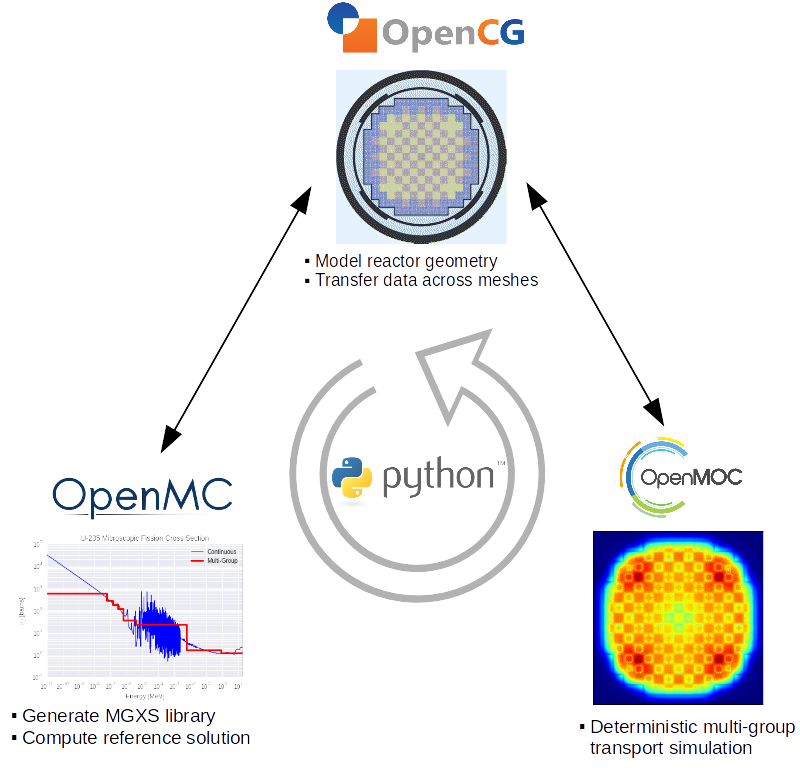
\includegraphics[width=0.8\linewidth]{figures/workflow/triad/simulation-triad}
\caption[A simulation triad of OpenMC, OpenMOC and OpenCG]{A simulation triad consisting of the OpenMC, OpenMOC and OpenCG codes ``glued'' together with Python formed the foundation for this thesis research.}
\label{fig:chap4-simulation-triad}
\end{figure}

This chapter describes the author's contributions to each component code in the simulation triad to support the objectives of this thesis -- namely, the evaluation of intrinsic bias in \ac{MGXS} for fine mesh transport (Chaps.~\Crefrange{chap:biases}{chap:sph}), and the development of a novel metholodogy for spatial homgenization based on unsupervised clustering (Chaps.~\Crefrange{chap:benchmarks}{chap:unsupervised}). An overview of the OpenMC, OpenMOC, and OpenCG codes, along with the features added to each code to support this thesis, are presented in Secs.~\ref{sec:chap4-openmc},~\ref{sec:chap4-openmoc}, and~\ref{sec:chap4-opencg}, respectively.

%The infrastructural code framework was developed using the Python programming language due to its flexibility and ease of use, as well as its extensive ecosystem of open source packages for high-performance data analysis.

%second paragraph: big data -> perhaps this should be in the motivation above?
%-explain/assume the need to tally across each spatial mesh zone
%-need to process large amounts of tally data
%-BEAVRS core figures for motivation
%-bulletize requirements?
%  -\# nuclides, \# tally regions, \# groups => data size
  
%third paragraph: requirements for software
%-processing/transferring lots of data
%  -requires a robust and scalable framework to ``glue'' triad together
%-requires extensions to each code

\begin{emphbox}
\textbf{A simulation triad consisting of OpenMC, OpenMOC and OpenCG was created to evaluate \ac{MGXS} generated from \ac{MC} within a Python-based framework.}
\end{emphbox}


%%%%%%%%%%%%%%%%%%%%%%%%%%%%%%%%%%%%%%%%%%%%%%%%%%%%%%%%%%%%%%%%%%%%%%%%%%%%%%%%
\section{OpenMC}
\label{sec:chap4-openmc}

The OpenMC code is a continuous energy Monte Carlo neutron transport code~\cite{romano2013openmc} with support for general constructive solid geometry models. OpenMC was initially created by Romano for his PhD thesis~\cite{romano2013parallel} to explore novel parallel algorithms for \ac{HPC} architectures. The code was released for public use with the MIT open source license, and has attracted growing interest as a platform for the development of new physics methods and computational algorithms. Although this thesis could have plausibly used any continuous energy \ac{MC} neutron transport code to generate \ac{MGXS}, this author chose OpenMC for its general and extensible implementation, excellent parallel scalability, and open source license agreement which permits the modification of its codebase. The general physics and computational methods implemented in OpenMC will not be detailed here since they are well documented in the literature. The interested reader is referred to the online code manual~\cite{openmc2016manual} for further information.

This thesis developed new features for OpenMC to enable the processing of large tally datasets to generate \ac{MGXS}. These contributions were motivated by the novel spatial homogenization technique presented in 
Chaps.~\Crefrange{chap:benchmarks}{chap:unsupervised} which required the calculation of microscopic \ac{MGXS} for each nuclide in each spatial zone across a reactor core geometry. The tally datasets for this scheme are orders of magnitude larger than those generated by the multi-level approaches previously considered in the literature. In particular, the tally datasets are computed on a fine (\textit{e.g.}, pin-wise) spatial tally mesh for a fully-detailed heterogeneous whole-core geometry. This stands in contrast to multi-level approaches which compute \ac{MGXS} for each unique fuel pin or assembly with infinite lattice boundary conditions for use in a multi-group whole-core calculation. For example, the scheme introduced here would tally \ac{MGXS} for each of the $\mathcal{O}(50,000)$ fuel pins in a whole-core \ac{MC} simulation of a \ac{PWR}. In contrast, a multi-level approach would compute \ac{MGXS} for the $\mathcal{O}(10)$ of unique fuel pins or assemblies in the model with pin-wise or assembly-wise \ac{MC} simulations.

This thesis' requirements for ``big data'' Monte Carlo calculations can be defined along two primary dimensions: scalable parallel algorithms for efficient \ac{MC} tracking, sampling and tallying, along with flexible and robust tools for downstream data processing. The first of these dimensions has been a focal point for OpenMC development since its inception. OpenMC includes distributed memory parallelism via the Message Passing Interface (MPI) and has been shown to scale with near perfect efficiency to 100,000s of processor cores~\cite{romano2013parallel}. In addition, shared memory parallelism is implemented with the OpenMP library~\cite{siegel2014multi} which reduces the simulation memory footprint by minimizing domain replication on multi-core processors. Furthermore, recent work has developed innovative schemes to manage tally datasets with memory footprints beyond that available on a single node in a typical \ac{HPC} machine (a few tens of gigabytes) with tally servers~\cite{romano2013servers} and spatial domain decomposition~\cite{horelik2014dd}. The efficient parallel algorithms already implemented in OpenMC were a key reason to use the code for this thesis work.

However, this thesis did involve the development of software tools to address the data processing needs for ``big data'' \ac{MC} calculations. It is the author's opinion that these data processing tools uniquely position OpenMC as the only \ac{MC} code presently capable of supporting the \ac{MGXS} generation scheme introduced in Chaps.~\Crefrange{chap:benchmarks}{chap:unsupervised}. For example, many commonly used \ac{MC} codes store and retrieve tally data from \ac{ASCII} formatted files or flat binary files. Although these file formats may work well for small tally datasets, they do not scale well for the tally datasets used in this thesis. The data processing paradigm reinforced by many \ac{MC} codes places an large burden on the user to write convoluted parsers to extract tally data without a generic set of tools to guide the process. In addition, many tally data stores are organized in a way that necessarily serializes tally data access without the metadata needed to index data in an efficient and parallel manner. Furthermore, many data stores are highly tailored to tallies on Cartesian or hexagonal meshes rather than the more complex unstructured meshes needed to generate \ac{MGXS} for fine mesh transport codes. The software tools developed for this thesis attempt to mitigate these issues and formalize a flexible and scalable tally data model for OpenMC.

%The development of a next-generation data model for OpenMC took a user-centric approach with the following three focus areas:

%\begin{itemize}[noitemsep]
%\item \textbf{Expressive Input} -- intuitive and compact simulation model descriptions
%\item \textbf{Managed Execution} -- automated optimization of simulation performance
%\item \textbf{Seamless Processing} -- scalable tools to index and transform tally data
%\end{itemize}

This section describes the features introduced to develop a next-generation tally data model in OpenMC and follows a recent paper by this author~\cite{boyd2016bigdata}. Sec.~\ref{subsec:chap4-py-api} presents a fully-featured Python \ac{API} for OpenMC which formed the foundation for much of this work. An algorithm to simplify tally management on unstructured but repeated tally volumes is highlighted in Sec.~\ref{subsec:chap4-distribcells}, and a feature to use isotropic in lab scattering is examined in Sec.~\ref{subsec:chap4-iso-in-lab}. Finally, a new module to generate \ac{MGXS} was implemented atop many of the newly introduced features in OpenMC as discussed in Sec.~\ref{subsec:chap4-mgxs}. All of the feature implementations were peer reviewed and incorporated into the v0.7.1 release of OpenMC.

%%%%%%%%%%%%%%%%%%%%%%%
\subsection{Python API}
\label{subsec:chap4-py-api}

A fully-featured Python \ac{API} was designed and implemented to enable programmatic pre- and post-processing for OpenMC. The \ac{API} enables tight coupling of input generation, simulation execution, and tally data analysis within dynamic Python script ``input files.'' In addition, the \ac{API} makes it possible to leverage the extensive ecosystem of Python packages for scientific computing alongside OpenMC in a simulation workflow. The following sections describe the \ac{API} and some of the core features which comprise the software stack developed to support the \ac{MGXS} generation module created for OpenMC.

%%%%%%%%%%%%%%%%%%%%%%%%%%%%%%%%%
\subsubsection{Overview}
\label{subsubsec:chap4-py-api-overview}

%-important to have flexible handle on the geometry for high-fidelity spatial tallies

The Python \ac{API} is a user-friendly, complementary (and optional) addition to the OpenMC codebase. OpenMC is written in Fortran 2008 and uses \ac{XML} input files to describe the simulation materials, geometry, tallies, and settings. Although \ac{XML} is often hailed as both human-readable and machine-readable, it is cumbersome to write by hand for large and complicated reactor models such as those modeled in this thesis. The Python \ac{API} circumvents this process by leveraging Python's internal \texttt{ElementTree} \ac{API} to generate the \ac{XML} files used by the OpenMC executable. Instead of writing \ac{XML} files by hand, dynamic Python scripts are used to describe one or more OpenMC simulations, including those used to generate \ac{MGXS} with OpenMC.

The OpenMC Python \ac{API} adheres to object-oriented software design principles with extensible class definitions. A user instantiates, manipulates, and connects objects representing items such as the materials, geometry and tallies to construct an OpenMC simulation. This is a scalable alternative workflow to traditional ``decks'' of ``cards'' in which data characterizing a simulation is specified in opaque \ac{ASCII} files (\textit{e.g.}, integer identifiers for geometric primitives such as surfaces, cells, universes, etc.). The Python \ac{API} provides classes and routines to represent all features provided by OpenMC's \ac{XML} input specifications.

In addition to its functionality for input generation, the Python \ac{API} also includes a rich framework of tally data processing utilities. The \ac{API} eliminates the time intensive and error prone process of writing code to parse results from OpenMC's output files. The \ac{API} is able to reconstruct the hierarchy of interconnected Python objects used to represent the materials, geometry and tallies from OpenMC's ``statepoint'' and ``summary'' \ac{HDF5} output files~\cite{koranne2011hdf5}. OpenMC's dynamic object-oriented data processing model -- fusing the geometry and materials configuration with tallied data -- enabled the rapid calculation, indexing and storage of \ac{MGXS} from tallies on unstructured meshes for this thesis.
  
%%%%%%%%%%%%%%%%%%%%%%%%%%%%%%%%%
\subsubsection{Pandas DataFrames}
\label{subsubsec:chap4-pandas-df}

The Python API encapsulates numerical tally data using $N$-dimensional array objects from the NumPy package~\cite{walt2011numpy}. Although OpenMC's NumPy interface to tally data is more flexible than simply reporting the data in \ac{ASCII} files, NumPy arrays are relatively opaque containers for managing large tally datasets. A single OpenMC \texttt{Tally} object used for \ac{MGXS} generation may encompass many different energy groups, nuclides and reaction types, yet all of this data is tabulated in a single contiguous NumPy array. As a result, it is challenging to implement general algorithms to inspect, index, and manipulate tally data in NumPy arrays for specific groups, nuclides or reactions.

The Pandas Python package~\cite{mckinney2010pandas} was implemented in the Python \ac{API} to enable transparent tally data processing for \ac{MGXS} generation. In particular, the \texttt{Tally} class includes a feature to construct a Pandas 
\texttt{DataFrame} object from tally data. Pandas \texttt{DataFrames} are modeled after data structures in the \textsf{R} programming language used to store data tables in a more accessible format than contiguous arrays. Pandas \texttt{DataFrames} support mixed-type data (\textit{i.e.}, strings and numbers), and allow the use of string keys or labels to index each column or row. The Python \ac{API} builds Pandas DataFrames by annotating tally data with the filters, nuclides, and scores associated with each tally bin. 

Pandas' most advanced features are intended for scalable data manipulation operations such as sorting, merging, and joining datasets, and generating pivot tables. In addition, Python's powerful statistics and machine learning packages -- such as SciPy~\cite{jones2011scipy}, statsmodels~\cite{seabold2010statsmodels} and scikit-learn~\cite{pedregosa2011sklearn} -- are well integrated with Pandas and may be easily applied to \texttt{DataFrames} of tally data. Pandas \texttt{DataFrames} were extensively used to encapsulate tally data throughout the statistical data processing framework for the \ac{MGXS} spatial homogenization methology introduced in Chaps.~\Crefrange{chap:benchmarks}{chap:unsupervised}.

%%%%%%%%%%%%%%%%%%%%%%%%%%%%%%%%
\subsubsection{Tally Slicing and Merging}
\label{subsubsec:chap4-tally-slice-merge}

Two useful and related features in the OpenMC Python \ac{API} for \ac{MGXS} generation are \textit{tally merging} and \textit{tally slicing} as depicted in Fig.~\ref{fig:tally-merge-slice}. It is intuitively useful to systematically create individual \texttt{Tally} objects for each spatial zone and reaction type when generating the OpenMC inputs necessary to compute \ac{MGXS}. However, this necessarily leads to a large number (10$^2$ -- 10$^3$) of distinct tally objects for large, complex geometries, which poses a computational bottleneck since the overhead to tally in OpenMC scales as $\mathcal{O}(N)$ for $N$ tallies. 

To compensate for this, the Python \ac{API}'s \texttt{Tally} class automatically merge user-specified tallies for input generation. Similarly, the \ac{API} supports the slicing of tallies to simplify downstream data processing which may comprise energy-, nuclide-, and/or reaction-dependent transformations of the tally data. Tally merging and slicing are extensively used throughout the statistical data processing framework for the \ac{MGXS} spatial homogenization methology introduced in Chaps.~\Crefrange{chap:benchmarks}{chap:unsupervised}.

\begin{figure}
\begin{subfigure}{\textwidth}
  \centering
  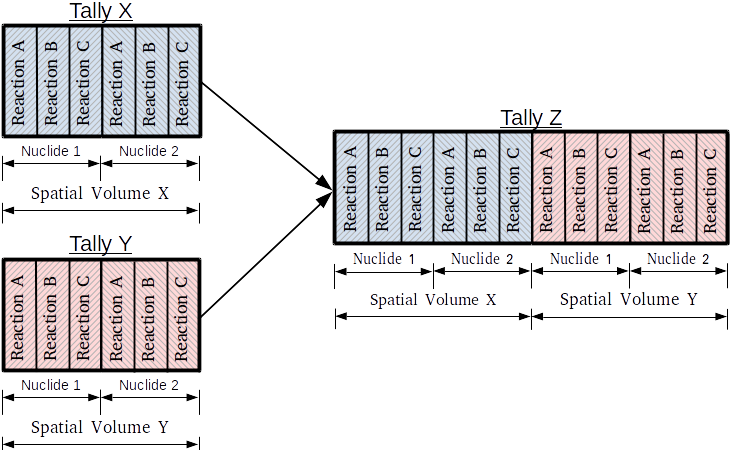
\includegraphics[width=\linewidth]{figures/workflow/openmc/tally-merge}
  \caption{}
\end{subfigure}
\begin{subfigure}{\textwidth}
  \centering
  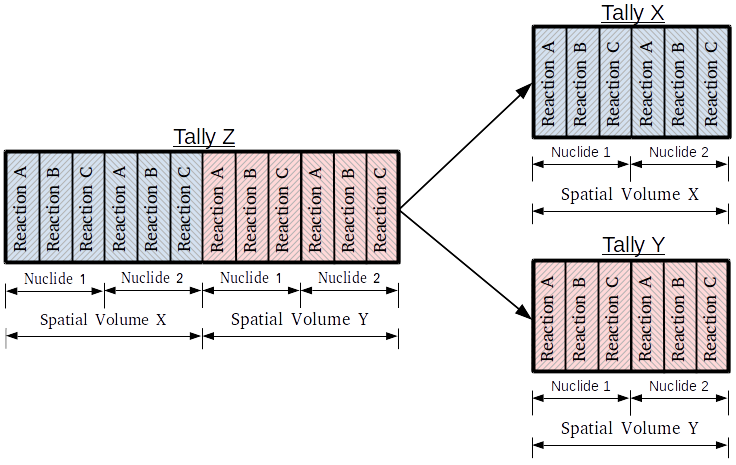
\includegraphics[width=\linewidth]{figures/workflow/openmc/tally-slice}
  \caption{}
\end{subfigure}
\caption[Tally merging and slicing operations]{Two \texttt{Tally} objects for different spatial volumes are merged into a single \texttt{Tally} (a). A single \texttt{Tally} is sliced by spatial volume into two distinct \texttt{Tally} objects (b).}
\label{fig:tally-merge-slice}
\end{figure}

%paragraph: aggregation (slicing/merging)
%-operations use NumPy to efficiently create derived sliced/merged tallies
%-slicing/merging can be used to slice tallies apart by nuclide, group, domain, etc.
%  -use tally merging to re-assembly MGXS from outputs of ML algorithms

%%%%%%%%%%%%%%%%%%%%%%%%%%%%%%%%
\subsubsection{Tally Arithmetic}
\label{subsubsec:chap4-tally-arithmetic}

As discussed in Sec.~\ref{subsec:chap3-tally-types}, a variety of reaction rate and flux tallies must be arithmetically combined in order to compute \ac{MGXS} with Monte Carlo (see Sec.~\ref{subsec:chap3-tally-types}). At the most general level, a reaction rate tally must be divided by a flux tally for each energy group, nuclide and tally volume (see Eqn.~\ref{eqn:chap3-general-micro}). In addition, the transport correction must be subtracted from the total cross section and scattering matrix (Eqns.~\ref{eqn:chap3-sigt-transport-macro} and~\ref{eqn:chap3-scatter-trans-macro}), and a summation must be performed over energy groups to compute the fission emission spectrum (Eqn.~\ref{eqn:chap3-chi}). Furthermore, it is desirable to compute a variance estimator for each \ac{MGXS} by propagating uncertainties as described in Sec.~\ref{subsec:chap3-uncertainty-prop}. The Python \ac{API} provides a novel feature known as \textit{tally arithmetic} to enable arithmetic combinations of tallies with efficient vectorized numerical operations across energy groups, nuclides and spatial tally zones.

Tally arithmetic is an object-oriented data processing feature which arithmetically combines two or more tallies and/or scalar values into new \textit{derived tallies}. The objective of tally arithmetic is to rapidly transform tally data with automated uncertainty propagation. The tally arithmetic implementation in OpenMC overloads the operators for addition, subtraction, multiplication, division, and exponentiation in the Python \ac{API}'s \texttt{Tally} class. In addition, the \texttt{Tally} class supports summation or averaging operations across some or all of its filter, nuclide or score bins.  The derived tallies produced from tally arithmetic provide the same rich functionality available for the \texttt{Tally} operands used in the arithmetic operation (\textit{e.g.}, Pandas DataFrames, tally arithmetic).

Multi-group cross sections may be simply and efficiently computed with tally arithmetic. For example, the following code snippet illustrates how tally slicing and arithmetic are used to compute a total \ac{MGXS}:

\lstinputlisting[language=Python, basicstyle=\ttfamily\scriptsize, caption={\ac{MGXS} calculation with tally arithmetic.}, label={lst:python-input}]{listings/workflow/tally-arithmetic.py}

\noindent The total \ac{MGXS} that is returned from the tally division operation is encapsulated within a \texttt{Tally} class. This is the approach used by the \ac{MGXS} generation module created for OpenMC in Sec.~\ref{subsec:chap4-mgxs}.

It should be noted that the uncertainty propagation in tally arithmetic makes the assumption that tallies represent independent random variables (see Sec.~\ref{subsec:chap3-uncertainty-prop}). However, in many if not most cases this assumption is untrue as tallies may be highly correlated. For example, there is a strong correlation between the flux and reaction rate tallies across the same material or cell, but this is not accounted for when these tallies are combined to compute \ac{MGXS} with tally arithmetic. In the future it may be possible to improve this approximation with the inclusion of tally covariance matrices in tally arithmetic.

%%%%%%%%%%%%%%%%%%%%%%%%%%%%%%%%%%%%%
\subsection{Distributed Cell Tallies}
\label{subsec:chap4-distribcells}

Many Monte Carlo codes, including OpenMC, use some variant of combinatorial geometry. because it can represent arbitrary, repeating geometries such as fuel pins and assemblies. However, the \ac{CG} approach is challenged by applications which require tallies in each instance of a repeated cell throughout a reactor geometry, such as the \ac{BEAVRS} benchmark model~\cite{horelik2013beavrs} depicted in Fig.~\ref{fig:beavrs}. The ``brute force'' solution is to instantiate a unique cell for each distinct tally zone. However, this defeats the purpose of using \ac{CG} for its compact representation, and it is not scalable to problems with large tally datasets such as those considered in this thesis.

\begin{figure}[h!]
  \centering
  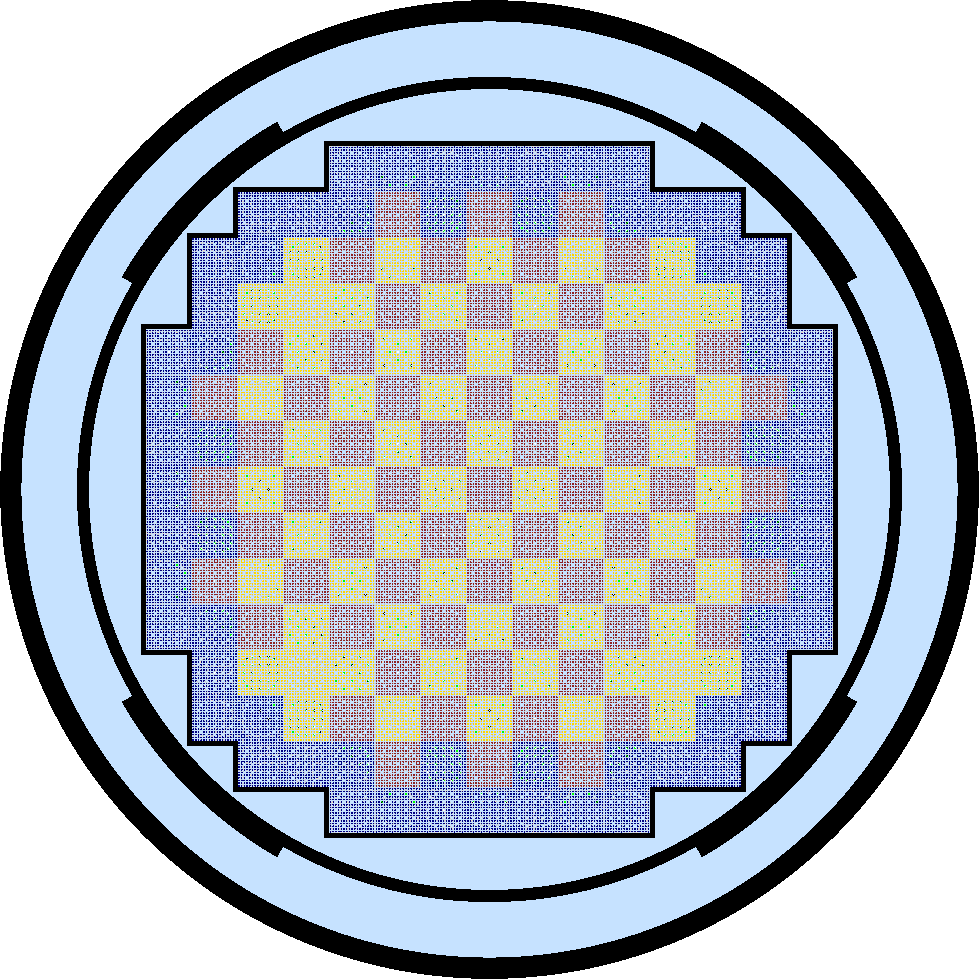
\includegraphics[width=2.5in]{figures/workflow/openmc/core}\hspace{1cm}
  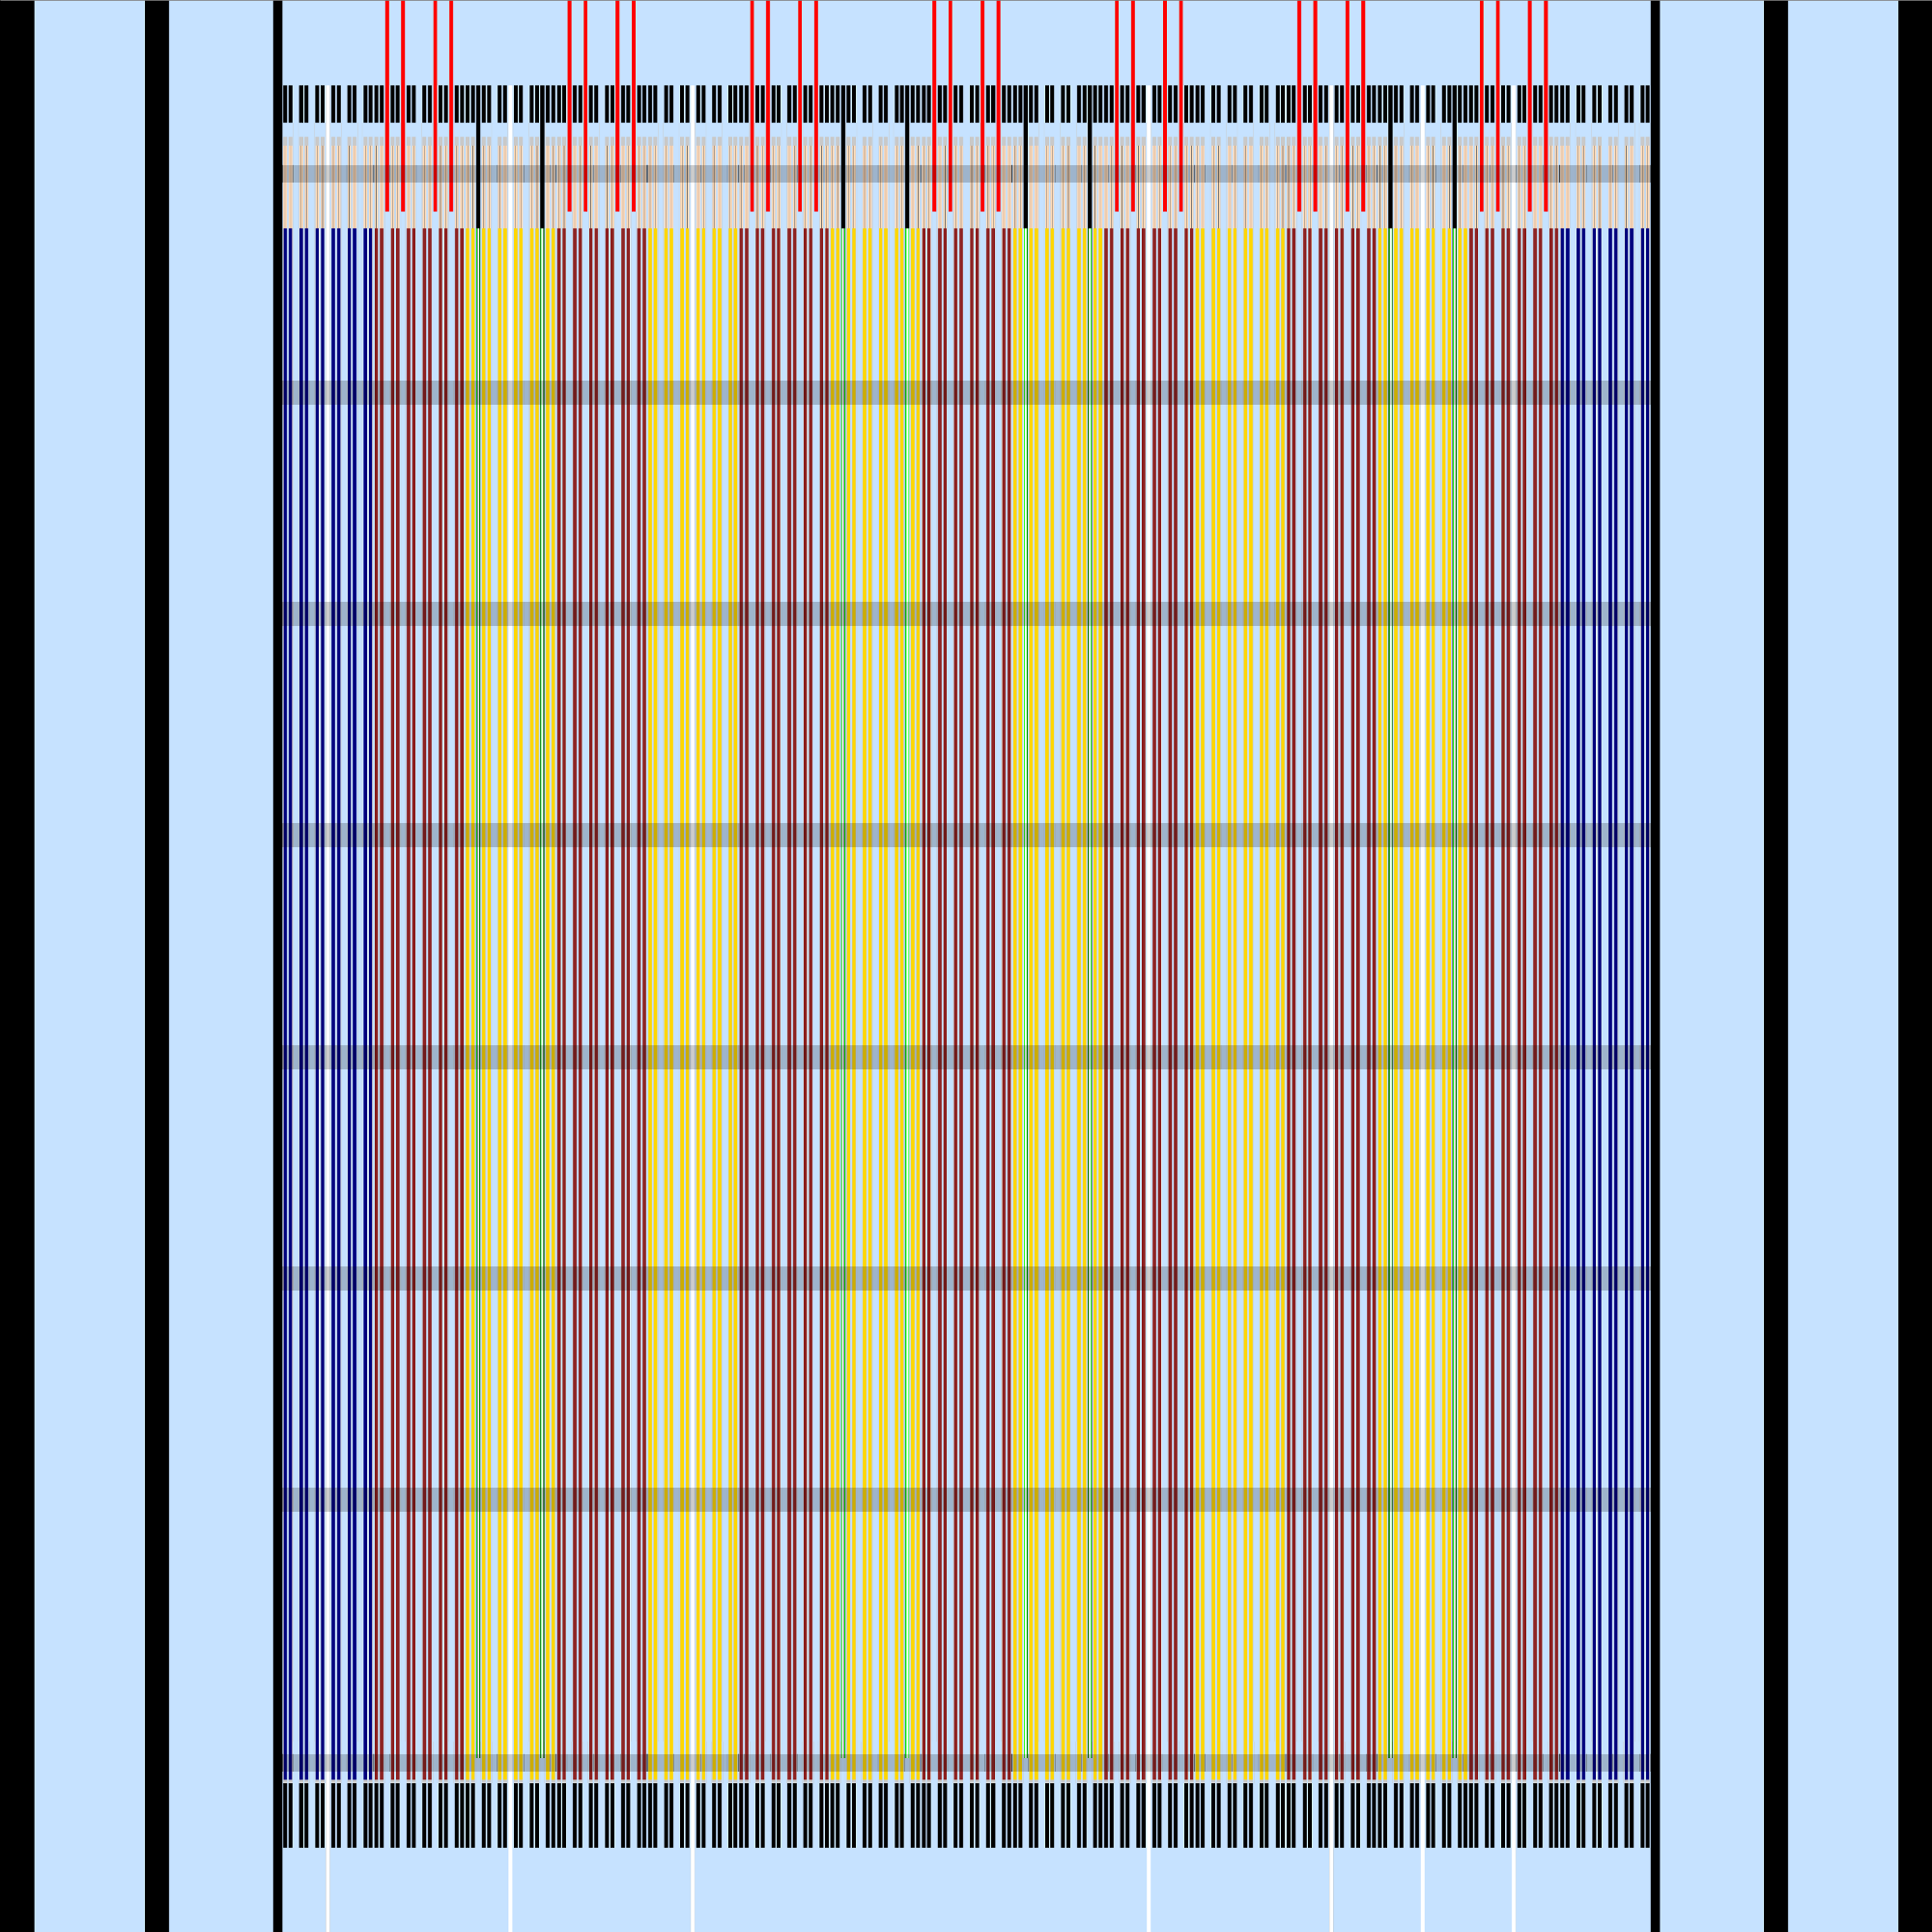
\includegraphics[width=2.5in]{figures/workflow/openmc/core_axial}
\caption[Radial and axial views of the BEAVRS core]{The radial (a) and axial (b) views of the BEAVRS \ac{PWR} core geometry~\cite{horelik2013beavrs}. The distributed cell tally algorithm provides a simple and efficient interface to tally within each of the 50,000+ fuel, guide tube, and burnable poison pin cells in complex heterogeneous models like the \ac{BEAVRS} core.}
\label{fig:beavrs}
\end{figure}

The \textit{distributed cell tally} algorithm was implemented in OpenMC to permit simply defined spatial tally zones across repeated cell instances~\cite{lax2014distribcell}. The distributed cell algorithm, commonly abbreviated as the \textit{distribcell} algorithm, classifies each unique cell instance using \textit{maps} and \textit{offsets} which consume orders of magnitude less memory than would be required by the ``brute force'' approach. Only a single transparent line of \ac{XML} input is necessary to define a distribcell tally which may span across an arbitrary number of instances for a particular cell. Furthermore, the Python \ac{API} may be used to perform efficient vectorized transformations of distribcell tally data stored as contiguous NumPy arrays. The distribcell tally algorithm was used to compute spatially-varying \ac{MGXS} across fuel pin cell instances for the spatial homogenization methology introduced in Chaps.~\Crefrange{chap:benchmarks}{chap:unsupervised}.

The distribcell tally algorithm consists of pre-processing and indexing stages. The pre-processing phase builds a mapping to index unique regions based on the unique combination of cells, universes and lattices used to construct each region. This is done by storing offset numbers in the data structures for each fill cell\footnote{Any cell that is filled with a nested universe or lattice of cells.}. The offset maps are recursively constructed starting from the top-level universe and proceeding through each lower nested universe level in the combinatorial geometry. The pre-processing algorithm tabulates the total number of instances of each cell in the geometry in order to dynamically allocate memory for distribcell tally arrays. At runtime, the on-the-fly indexing scheme efficiently computes cell instance IDs in order to index and score to the appropriate bin(s) in distribcell tallies. The cell instance IDs are simply found by summing the offsets at each nested universe level along the path to the cell instance in the \ac{CG} as shown in Fig.~\ref{fig:indexing-scheme}. The interested reader is referred to~\cite{lax2014distribcell} for details about the distribcell tally algorithm, including pseudocode for pre-processing and indexing and a performance model for the memory footprint consumed by offsets and maps.

\begin{figure}
  \centering
  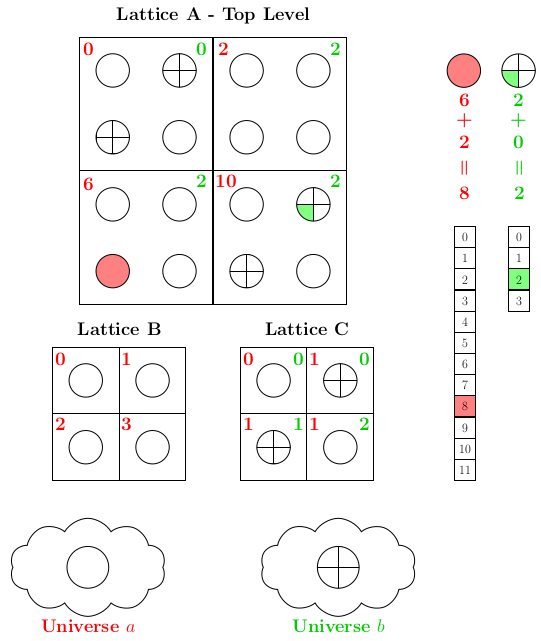
\includegraphics[width=\linewidth]{figures/workflow/openmc/distribcells}
\caption[The distributed cell tally indexing algorithm]{An example of the distribcell tally algorithm's on-the-fly indexing scheme~\cite{lax2014distribcell}. Material-filled cells are defined in pin cell universes $a$ and $b$, which are filled into the cells of lattices $B$ and $C$, which are filled into the cells of lattice $A$.  The colored numbers in each fill cell are the offsets for each base universe, which can be used to quickly compute a unique ID for each instance of a material cell.}
\label{fig:indexing-scheme}
\end{figure}

%%%%%%%%%%%%%%%%%%%%%%%%%%%%%%%%%%%%%%%%
\subsection{Isotropic in Lab Scattering}
\label{subsec:chap4-iso-in-lab}

As part of this thesis, a unique option for isotropic in lab scattering was implemented in the OpenMC code. The isotropic in lab (abbreviated as iso-in-lab) feature may be useful to quantify the ability of multi-group codes to capture anisotropic scattering effects with higher order scattering matrices or transport correction schemes (see Sec.~\ref{subsec:chap2-transport-corr}). The iso-in-lab scattering feature was implemented as a ``scattering'' attribute for each nuclide/element in a simulation. When iso-in-lab scattering is specified for a nuclide/element, the outgoing neutron energy is sampled from the scattering laws prescribed by the continuous energy cross section library, but the outgoing neutron direction of motion is sampled from an isotropic in lab distribution. 

Unless otherwise noted, isotropic in lab scattering was employed in OpenMC to generate the \ac{MGXS} used in this thesis. The iso-in-lab scattering feature enabled ``apples-to-apples'' comparisons between the reference eigenvalues and reaction rates produced by OpenMC and those computed from isotropic multi-group calculations with OpenMOC.

%%%%%%%%%%%%%%%%%%%%%%%%%%%%
\subsection{MGXS Generation}
\label{subsec:chap4-mgxs}

The OpenMC Python \ac{API}'s \texttt{openmc.mgxs} module was implemented to generate multi-group cross sections. The \texttt{openmc.mgxs} module is built atop the underlying core features in the rest of the \ac{API} to support a seamless interface for both input generation and downstream data processing of \ac{MGXS} from Python. In particular, one may specify the \ac{MGXS} to compute and the \texttt{openmc.mgxs} module will construct the necessary \texttt{Tally} objects. The \texttt{Tally} objects may be easily exported to \ac{XML} input files for OpenMC, and used to containerize and process the tally data produced by an OpenMC simulation. The \texttt{openmc.mgxs} module thereby leverages the software stack of Pandas DataFrames, tally arithmetic, etc. provided by the OpenMC Python \ac{API}.

The \texttt{openmc.mgxs} module can compute macroscopic or microscopic \ac{MGXS} for individual nuclides or elements as well as collections of nuclides and elements\footnote{A \ac{MGXS} computed for a collection of nuclides/elements is the sum of the individual contributions from each nuclide/element.}. \ac{MGXS} can be computed in one or more arbitrary energy group structures. The module supports energy condensation in downstream data processing which is useful for exploring approximation bias in various energy group structures. For example, \ac{MGXS} may be computed in a 16-group structure and the tally data subsequently condensed to 2-group, 8-group, 12-group, etc. structures for multi-group calculations\footnote{Energy condensation may be performed to arbitrarily defined coarse group structures with \texttt{openmc.mgxs} provided the coarse group boundaries coincide with boundaries in the fine group structure.}. The analysis in this thesis computed \ac{MGXS} in the 70-group structure provided in Tab.~\ref{table:app-70-groups}, and condensed the \ac{MGXS} to the coarser group structures given in Appendix~\ref{app:energy-groups} as needed.

The \texttt{openmc.mgxs} module is designed to perform spatial homogenization on heterogeneous tally meshes for fine mesh transport codes. In OpenMC parlance, \ac{MGXS} may be computed for material, cell or universe spatial domains. In addition, the module supports \ac{MGXS} calculations for repeated cell instances using distribcell spatial tally domains (see Sec.~\ref{subsec:chap4-distribcells}). The \texttt{openmc.mgxs} module may also perform spatial homogenization on structured Cartesian tally meshes for coarse mesh multi-gropu calculations. This thesis computed \ac{MGXS} using distribcell tallies (\textit{e.g.}, \ac{MGXS} for each fuel pin instance in a geometry) to support the \ac{MGXS} spatial homogenization introduced in Chaps.~\Crefrange{chap:benchmarks}{chap:unsupervised}.

The \texttt{openmc.mgxs} module uses an object-oriented design based on an abstract \texttt{MGXS} class with subclasses for different reaction types. The \texttt{MGXS} subclasses are itemized in Tab.~\ref{table:chap4-mgxs-types} and compute multi-group constants from \ac{MC} tallies using the methods detailed in Sec.~\ref{subsec:chap3-tally-types}. It should be noted that some reaction types include variants which do or do not account for scattering multiplicity reactions (see Sec.~\ref{sec:chap2-scatt-prod}). For example, the transport correction used by the \texttt{TransportXS} class does not include $(n,xn)$ reactions while that employed by the \texttt{NuTransportXS} does account for scattering multiplicity. The \texttt{openmc.mgxs} module also includes a \texttt{Library} class which automates the construction of \texttt{MGXS} objects for different group structures, spatial domains, and reaction types.

\begin{table}[h!]
  \centering
  \caption[The MGXS types implemented for OpenMC]{The \ac{MGXS} types implemented by the \texttt{openmc.mgxs} module in OpenMC.}
  \small
  \label{table:chap4-mgxs-types} 
  \vspace{6pt}
  \begin{tabular}{l p{10cm}}
  \toprule
  \rowcolor{lightgray}
  {\bf Class} &
  {\bf Description} \\
  \midrule
  \texttt{TotalXS} & Total collision \\
  \texttt{TransportXS} & Transport-corrected total collision \\
  \texttt{NuTransportXS} & Transport-corrected total collision w/ scattering multiplicity \\
  \texttt{AbsorptionXS} & Absorption \\
  \texttt{CaptureXS} & Radiative capture \\
  \texttt{FissionXS} & Fission \\
  \texttt{NuFissionXS} & Fission production \\
  \texttt{KappaFissionXS} & Fission energy release \\
  \texttt{ScatterXS} & Scattering \\
  \texttt{NuScatterXS} & Scattering w/ scattering multiplicity \\
  \texttt{ScatterMatrixXS} & Scattering matrix \\
  \texttt{NuScatterMatrixXS} & Scattering matrix w/ scattering multiplicity \\
  \texttt{Chi} & Fission emission spectrum \\
  \texttt{ChiPrompt} & Prompt fission emission spectrum \\
  \bottomrule
\end{tabular}
\end{table}

The \texttt{openmc.mgxs} module was developed with general design principles to generate \ac{MGXS} for any multi-group neutron transport code. Although the module does not explicitly support any multi-group codes, it can export \ac{MGXS} data to a variety of data storage formats, including \ac{CSV} and \ac{HDF5}. The exported \ac{MGXS} files may be easily transformed into the database or input files required by a particular multi-group code. As discussed in the following section, this thesis developed a tightly integrated framework to pipeline \ac{MGXS} generated by \texttt{openmc.mgxs} into the multi-group OpenMOC code.

\begin{emphbox}
\textbf{The OpenMC code was used to generate \ac{MGXS}. A Python \ac{API} was implemented for input generation and data processing, along with features including distributed cell tallies and isotropic in lab scattering. The \texttt{openmc.mgxs} Python module was created to generate \ac{MGXS} from OpenMC tallies.}
\end{emphbox}


%%%%%%%%%%%%%%%%%%%%%%%%%%%%%%%%%%%%%%%%%%%%%%%%%%%%%%%%%%%%%%%%%%%%%%%%%%%%%%%%
\section{OpenMOC}
\label{sec:chap4-openmoc}

The OpenMOC code is a multi-group neutron transport code implementing the deterministic Method of Characteristics (MOC)~\cite{boyd2014openmoc}. OpenMOC was initially developed to support a series of M.S. theses at MIT~\cite{li2013ms,boyd2014ms,shaner2014ms} and was later released for public use with the MIT open source license. Although this thesis could have plausibly used any multi-group code, OpenMOC was chosen for its flexible Python interface, computationally efficient algorithms, and the author's familiarity with the open source codebase.

%-reference need for MG code to evaluate MGXS for this thesis

This thesis inspired the development of new features and extensions which have been incorporated into the official OpenMOC codebase. This section begins with a brief overview of the \ac{MOC} implementation in OpenMOC in Sec.~\ref{subsubsec:chap4-openmoc-overview}. Various improvements were made to the OpenMOC Python interface as discussed in Sec.~\ref{subsubsec:chap4-openmoc-python}, while Sec.~\ref{subsubsec:chap4-openmoc-mgxs} details a module created to interface with \ac{MGXS} generated by OpenMC. The parallel algorithms and numerical acceleration schemes in OpenMOC which were used by this thesis are mentioned in Secs.~\ref{subsubsec:chap4-openmoc-parallel} and~\ref{subsubsec:chap4-openmoc-cmfd}, respectively.

%-improvements to the parallelism, CMFD to enable ``multi-sim'' calculations

%%%%%%%%%%%%%%%%%%%%%%%%%%%%%%%%%
\subsection{Methods Overview}
\label{subsubsec:chap4-openmoc-overview}

The method of characteristics is a widely used technique for solving partial differential equations, including the Boltzmann form of the neutron transport equation~\cite{askew1972moc}. Although not a stochastic formulation, \ac{MOC} is a ray-based algorithm akin to Monte Carlo particle tracking-based methods. In contrast to Monte Carlo, \ac{MOC} uses a fixed angular quadrature that is determined \textit{a priori}. This quadrature is used to specify 1D characteristics that cross the spatial domain. Prior to the physics computation, ray tracing must be performed to subdivide each characteristic into segments within different regions in the spatial mesh. Fig.~\ref{fig:moc-model} illustrates the spatial mesh and cyclic characteristic laydown used by the OpenMOC code.

\ac{MOC} propagates the angular neutron flux along each characteristic through each spatial zone. For each segment, the angular flux is attenuated due to neutron absorption and enhanced due to neutron fission or scattering in the corresponding spatial zone. \ac{MOC} uses the multi-group energy approximation such that this computation is performed for neutrons within discretized energy groups (see Sec.~\ref{subsec:chap2-energy}). Finally, an angular quadrature is applied to combine the average angular flux contribution from each characteristic to compute the average scalar flux in each zone and energy group.

\begin{figure}[h!]
  \begin{subfigure}[htb!]{0.32\textwidth}
    \centering
    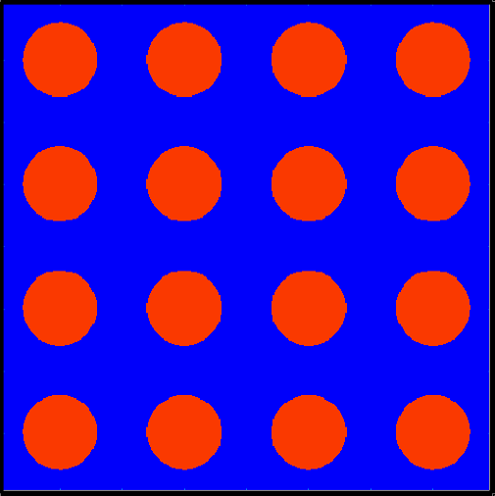
\includegraphics[width=0.95\textwidth]{figures/workflow/openmoc/materials-border}
    \label{fig:moc-model-materials}
    \caption{}
  \end{subfigure}
  \begin{subfigure}[htb!]{0.32\textwidth}
    \centering
    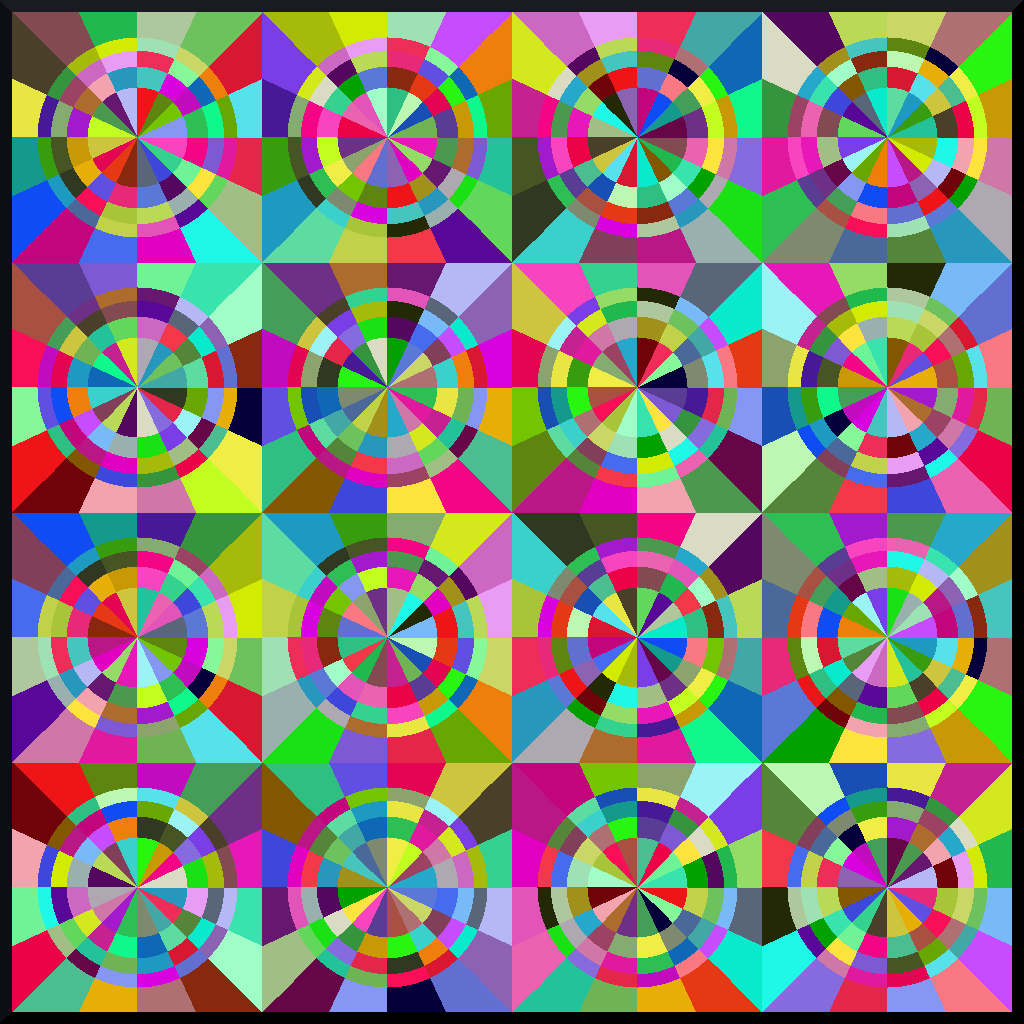
\includegraphics[width=0.95\textwidth]{figures/workflow/openmoc/FSRs}
    \label{fig:moc-model-fsrs}
    \caption{}
  \end{subfigure}
  \begin{subfigure}[htb!]{0.32\textwidth}
    \centering
    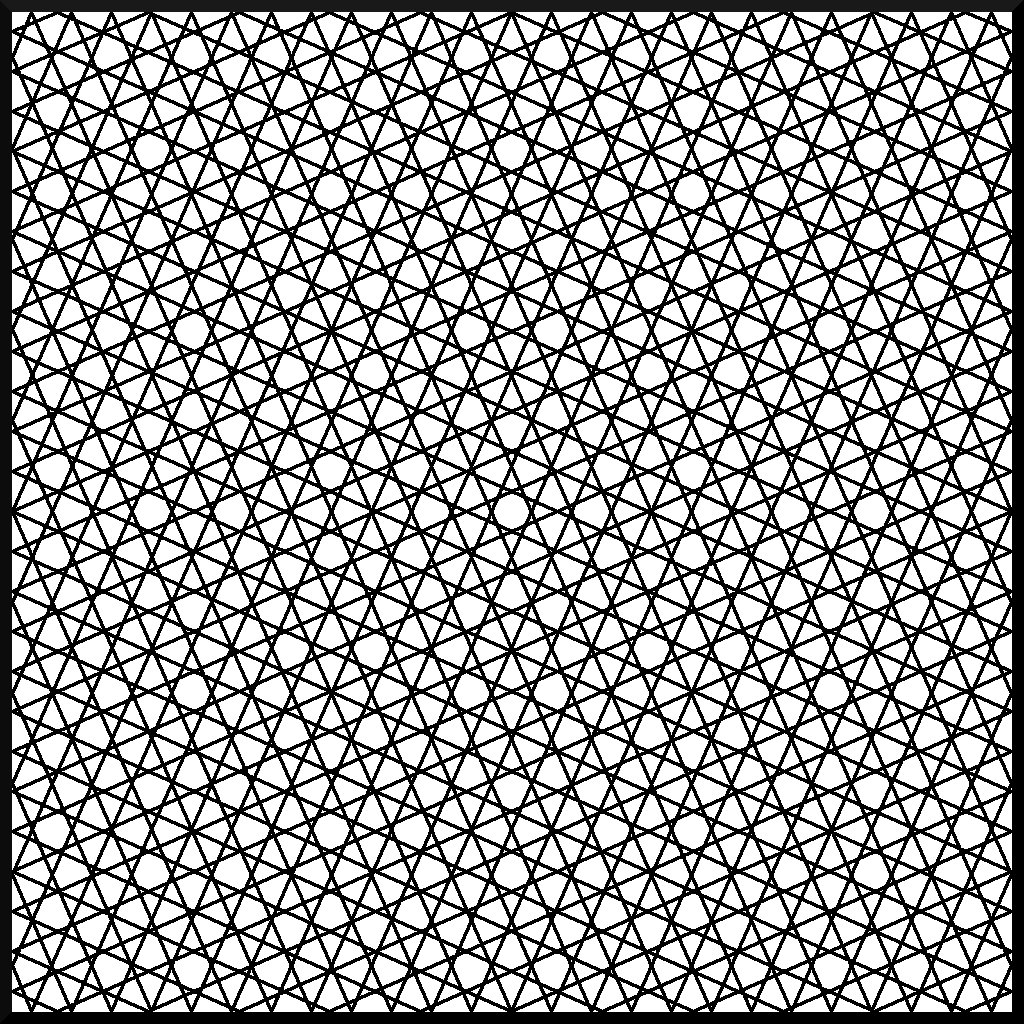
\includegraphics[width=0.95\textwidth]{figures/workflow/openmoc/cyclic-tracks}
    \label{fig:moc-model-tracks}
    \caption{}
  \end{subfigure}
\caption[Example OpenMOC flat source region mesh and track laydown]{The coolant and fuel materials (a), flat source region spatial mesh (b), and cyclic characteristic laydown (c) for a 4 $\times$ 4 fuel pin lattice taken from~\cite{boyd2016parallel}.}
\label{fig:moc-model}
\end{figure}

The OpenMOC code is capable of performing 2D \ac{MOC} calculations for light water reactor core configurations. OpenMOC discretizes the 2D geometry into flat source regions (FSRs) which approximate the neutron source as constant across each spatial zone\footnote{The neutron source may include any combination of fission, scattering and fixed sources.}. Furthermore, OpenMOC approximates the scattering source as isotropic in the lab coordinate system and is not yet able to use higher order scattering moment matrices. OpenMOC uses a power iteration scheme to solve for the dominant eigenvalue and eigenvector in criticality calculations. As part of this thesis, a general purpose fixed source solver was implemented to enable the detailed investigation of approximation bias in \ac{MGXS} as discussed in Chap.~\ref{chap:sph}. The interested reader is referred to the online code manual~\cite{openmoc2016manual} for more information detailing the \ac{MOC} implementation in OpenMOC.

%%%%%%%%%%%%%%%%%%%%%%%%%%%%%%%%%
\subsection{Python Interface}
\label{subsubsec:chap4-openmoc-python}

One of the key reasons that OpenMOC was used by this thesis was to leverage its flexible Python interface. The majority of the source code is written in C++ using object-oriented software design principles. The \ac{SWIG}~\cite{beazley2003swig} is deployed to expose the C++ classes and routines to the Python scripting language. The Python interface made it possible to tightly couple OpenMOC with the rich ecosystem of Python-based data processing and visualization tools for the spatial homogenization methodology developed in Chaps.~\Crefrange{chap:benchmarks}{chap:unsupervised}.

As part of this work, a new scheme was implemented to efficiently link OpenMOC's Python and C++ \ac{CG} data structures into a hierarchical tree-like data structure. This made it possible to use the OpenCG region differentiation algorithm discussed in Sec.~\ref{sec:chap4-region-diff} to derive geometries for OpenMOC. In addition, a thread-safe memory management model was realized which unifies the dynamic deallocation of objects shared between Python and C++ code. The memory model enabled 100s of OpenMOC simulations to be orchestrated by Python for the parametric studies considered in this thesis.

%\begin{figure}[h!]
%  \centering
%  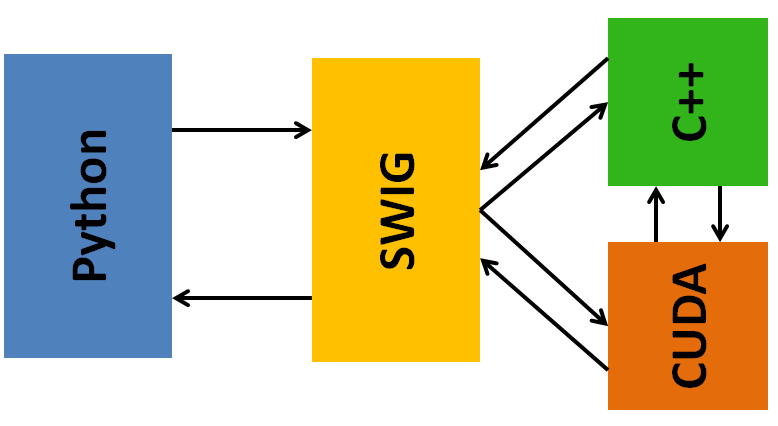
\includegraphics[width=0.7\linewidth]{figures/workflow/openmoc/software-design}
%\caption[The OpenMOC programming model]{The programming model used by OpenMOC to couple compiled C/C++/CUDA code to the Python interface using \ac{SWIG} taken from~\cite{boyd2014openmoc}.}
%\label{fig:openmoc-swig}
%\end{figure}

%%%%%%%%%%%%%%%%%%%%%%%%%%%%%%%%%
\subsection{Multi-Group Cross Sections}
\label{subsubsec:chap4-openmoc-mgxs}

OpenMOC uses multi-group macroscopic nuclear cross sections specified in any arbitrary energy group structure. Isotropic concentrations are not used since OpenMOC does not perform self-shielding or depletion calculations. Multi-group cross sections may be specified for each material or cell in the \ac{CG} used in a simulation. OpenMOC requires total, fission production and scattering matrix cross sections along with a fission emission spectrum\footnote{Transport-corrected total cross sections and scattering matrices may be used in OpenMOC.}. In addition, a fission cross section may be optionally supplied in order to compute spatially-varying fission reaction rates.

Cross section data is encapsulated by the \texttt{Material} class. A \texttt{Material} object may be instantiated in Python and cross section data loaded into it from NumPy arrays~\cite{walt2011numpy}. For simulations with many different materials (such as those in this thesis), defining nuclear cross section data by hand in a Python script is cumbersome and error prone. In order to minimize this painstaking process, the \texttt{openmoc.materialize} module was implemented to automate the loading \ac{MGXS} data into OpenMOC \texttt{Material} objects. This module can either import \ac{MGXS} data from HDF5 binary files~\cite{koranne2011hdf5} or extract \ac{MGXS} data from OpenMC \texttt{Library} Python objects (see Sec.~\ref{subsec:chap4-mgxs}). The \texttt{openmoc.materialize} module is designed to support large \ac{MGXS} libraries such as those produced from the spatial homogenization methodology introduced in Chaps.~\Crefrange{chap:benchmarks}{chap:unsupervised}. In addition, a scheme to compute \ac{SPH} factors to ensure reaction rate consistency with OpenMC was implemented in \texttt{openmoc.materialize} and is discussed in detail in Chap.~\ref{chap:sph}.

%%%%%%%%%%%%%%%%%%%%%%%%%%%%%%%%%
\subsection{Parallelism}
\label{subsubsec:chap4-openmoc-parallel}

OpenMOC's high performance parallel solvers for both multi-core \ac{CPUs} and \ac{GPUs} were extensively used for the analyses presented in this thesis. A shared memory parallel solver implemented in C++ using OpenMP~\cite{openmp2013} has demonstrated excellent scalability on a range of multi-core architectures\cite{boyd2016parallel}. In addition, OpenMOC includes a highly parallel implementation which uses the CUDA programming language~\cite{nvidia2012cuda} to run on NVIDIA \ac{GPUs} with 100s to 1000s of lightweight cores~\cite{boyd2013massively}. OpenMOC's parallel solvers made it possible to perform large parametric studies of 100s of \ac{MOC} simulations to evaluate the spatial homogenization methodology introduced in Chaps.~\Crefrange{chap:benchmarks}{chap:unsupervised}.


%%%%%%%%%%%%%%%%%%%%%%%%%%%%%%%%%
\subsection{CMFD Acecleration}
\label{subsubsec:chap4-openmoc-cmfd}

OpenMOC uses the Coarse Mesh Finite Difference (CMFD) acceleration scheme to greatly reduce the number of iterations required to converge criticality calculations~\cite{boyd2014openmoc}. \ac{CMFD} acceleration functions by using the solution of a coarse mesh diffusion problem to accelerate the convergence of the fine mesh \ac{MOC} transport problem. The details of the \ac{CMFD} implementation in OpenMOC are beyond the scope of this thesis, and the interested reader is referred to the online code manual~\cite{openmoc2016manual} for more information. 

\ac{CMFD} acceleration was extensively used to accelerate the eigenvalue calculations in this thesis. All simulations which employed \ac{CMFD} used the novel $k$-Nearest Neighbors prolongation scheme created by Shaner~\cite{shaner2015cmfd} and implemented in OpenMOC to improve the convergence rate and stability of \ac{CMFD}. In particular, all simulations used three neighbors along with a successive over-relaxation (SOR) factor of unity. Along with OpenMOC's parallel solvers, \ac{CMFD} acceleration made it feasible to perform large parametric studies to generate the results presented in this thesis.

%\begin{figure}[h!]
%  \centering
%  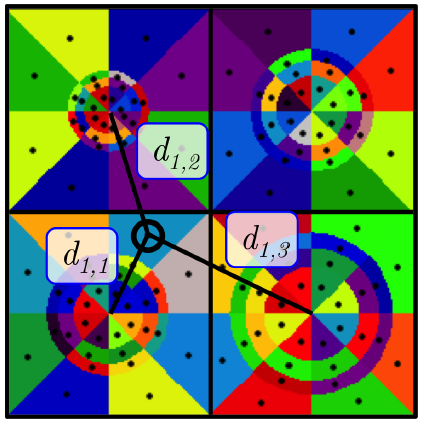
\includegraphics[width=0.5\linewidth]{figures/workflow/openmoc/centroid}
%\caption[$k$-nearest neighbor centroid scheme for CMFD]{The $k$-nearest neighbor centroid update scheme for \ac{CMFD}~\cite{shaner2015cmfd}.}
%\label{fig:knn-cmfd}
%\end{figure}

\begin{emphbox}
\textbf{The OpenMOC code was used to perform 2D deterministic multi-group \ac{MOC} calculations. The \texttt{openmoc.materialize} module was improved to support \ac{MGXS} generated from OpenMC. OpenMOC's parallel algorithms and \ac{CMFD} acceleration enabled parametric studies of 100s of OpenMOC simulations.}
\end{emphbox}


%%%%%%%%%%%%%%%%%%%%%%%%%%%%%%%%%%%%%%%%%%%%%%%%%%%%%%%%%%%%%%%%%%%%%%%%%%%%%%%%
\section{OpenCG}
\label{sec:chap4-opencg}

The OpenCG code~\cite{boyd2015opencg} was created to simplify the process of creating and transferring data mapped to combinatorial geometries for OpenMC and OpenMOC. Combinatorial geometry\footnote{\ac{CG} is often referred to as constructive solid geometry in the neutron transport literature.} is commonly used by neutron transport simulation codes since it:

\begin{itemize}[noitemsep]
  \item Permits description of an \textit{arbitrarily accurate} unstructured geometric mesh
  \item Provides a \textit{compact representation} with minimal input description
  \item Represents $\mathcal{O}(n)$ components with $\mathcal{O}(\log{}n)$ memory requirements
  \item Utilizes a hierarchical \textit{tree data structure} with scalable $\mathcal{O}(\log{}n)$ traversals
\end{itemize}

\noindent Although many codes utilize \ac{CG}, it is overly burdensome to manually write geometric input files for multiple simulation tools for code verification of a single reactor model. In addition, the compact geometric representation is not well-suited for large scale analysis of spatially-varying data in nuclear reactor cores -- such as distributed cell tally data in OpenMC -- without new algorithms to guide and automate the process. This thesis developed a new \ac{CG} modeling tool called OpenCG to accelerate the building of complicated reactor geometries, enable rapid cross-code verification and facilitate large scale data processing. 

OpenCG is a simple-to-use Python library which may be used to construct a single geometry for use in both OpenMC and OpenMOC. In addition, OpenCG enables data transfer between OpenMC and OpenMOC as illustrated in Fig.~\ref{fig:chap4-simulation-triad}. In particular, OpenCG accomodates the generation of \ac{MGXS} from distributed cell tallies on OpenMC's \ac{CG} mesh and maps them to the flat source region spatial mesh used by OpenMOC. A variant of OpenMC's distributed cell tally algorithm (see Sec.~\ref{subsec:chap4-distribcells}) was implemented in OpenCG to make this possible. In addition to transferring \ac{MGXS} data, OpenCG enabled the comparison of pin-wise reaction rate distributions computed from OpenMC distribcell tallies with those computed on OpenMOC's \ac{FSR} mesh.

The following sections outline the key features implemented in OpenCG for this thesis and follows a recent paper by this author~\cite{boyd2015opencg}. Sec.~\ref{sec:chap4-opencg-compatibility} discusses the compatibility modules which tie OpenCG, OpenMC and OpenMOC into a simulation triad. In addition, two novel algorithms known as \ac{LNS} and region differentiation were developed in OpenCG to enable the spatial homogenization methodology introduced in this thesis, and are presented in Secs.~\ref{sec:chap4-lns} and~\ref{sec:chap4-region-diff}, respectively.

%%%%%%%%%%%%%%%%%%%%%%%%%%%%%%%%%%%%
\subsection{Compatiblity Modules}
\label{sec:chap4-opencg-compatibility}

The simulation triad of OpenCG, OpenMC and OpenMOC shown in Fig.~\ref{fig:chap4-simulation-triad} is made possible with compatibility modules. The compatibility modules allow the construction of a single geometry using OpenCG's Python \ac{CG} primitives for surfaces, cells, universes and lattices. The OpenCG geometry may then be exported to OpenMC or OpenMOC using compatibility modules developed for each code.

For example, OpenMC includes a Python \ac{API} with object-oriented \ac{CG} primitives. This \ac{API}'s primitives include routines to directly export themselves to the \ac{XML} input file format used by OpenMC. The OpenCG-OpenMC compatibility module allows OpenCG's primitives to be transformed into the corollaries within the OpenMC Python \ac{API}, and vice versa. Likewise, the OpenCG-OpenMOC compatibility module allows OpenCG's primitives to be transformed into the corollaries within the OpenMOC Python/C++ code. In summary, the compatibility modules enable the rapid, automated exportation of various OpenCG geometries directly to OpenMC and OpenMOC.

OpenCG's object-oriented Python software model permits greater freedom for geometric parameter optimization than can be easily achieved with traditional \ac{ASCII} or \ac{XML} input files. In particular, the compatibility module framework enabled a dynamic workflow between OpenMC and OpenMOC for \ac{MGXS} generation and code verification in this thesis. For example, OpenCG's region differentiation algorithm (see Sec.~\ref{sec:chap4-region-diff}) was used to produce 100s of geometries composed with different \ac{MGXS} libraries to evaluate the spatial homogenization methodology introduced in Chaps.~\Crefrange{chap:benchmarks}{chap:unsupervised}.

%\begin{figure}[h!]
%  \centering
%  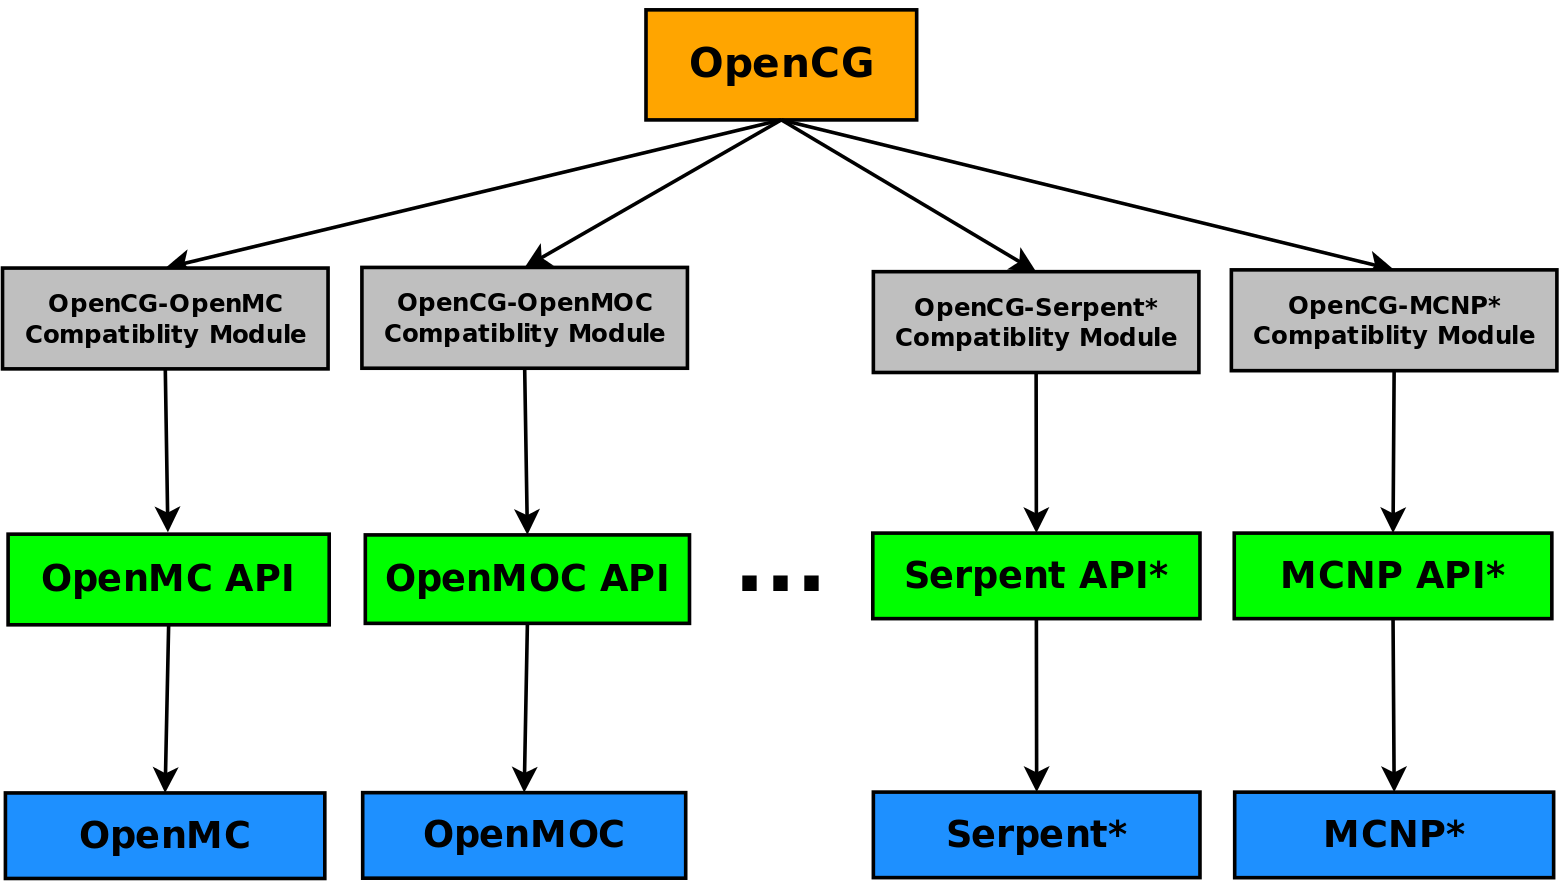
\includegraphics[width=.8\linewidth]{figures/workflow/opencg/compatibility-modules}
%  \caption{OpenCG compatibility modules for various neutron transport codes. The compatibility modules for OpenMC and OpenMOC will be released in future public distributions of each code, while modules for Serpent and MCNP are in progress at the time of this writing.}
%  \label{fig:compatibility-modules}
%\end{figure}


%%%%%%%%%%%%%%%%%%%%%%%%%%%%%%%%%%%%
\subsection{Local Neighbor Symmetry}
\label{sec:chap4-lns}

One of the unique algorithms implemented in OpenCG explicitly for this thesis is known as Local Neighbor Symmetry (LNS) identification~\cite{boyd2015opencg}. The LNS algorithm is motivated by this thesis' objective to accurately predict spatial zones that experience similar spectral self-shielding effects. The \ac{LNS} algorithm performs a systematic analysis of a \ac{CG} tree data structure to identify neighbor cells, or pairs of cells which are adjacent to one another. The neighbor cells are assembled into a heuristic which groups like spatial zones with common \ac{LNS} identifiers. The \ac{LNS} algorithm is analogous to the geometric templates used in lattice physics codes such as CASMO~\cite{edenius1995casmo} to identify fuel pins which have similar \ac{MGXS} in a fuel assembly.

The \ac{LNS} algorithm identifies the unique symmetry for the path to a region in a combinatorial geometry as described in Alg.~\ref{alg:local-neighbor-symmetry-cells}. \ac{LNS} performs a \ac{BFS} to find neighbors on each level of the \ac{CG} tree. For example, \ac{BFS} is used to find neighbor cells for a particular cell within a universe. Similarly, \ac{BFS} is used to find neighbor universes adjacent to a particular lattice cell. The neighbor cells and universes on each of the $k$ levels of a \ac{CG} tree are connected to form a $k$-partite graph\footnote{A $k$-partite graph is a graph whose graph vertices can be partitioned into $k$ disjoint sets so that no two vertices within the same set are adjacent~\cite{weisstein2012kpartite}.} as depicted in Fig.~\ref{fig:lns-k-partite-graph}. Finally, the $k$-partite graph is used as an argument to a hash function to compute the \ac{LNS} identifier (\textit{e.g}, a non-negative integer) for the particular region represented by the path. This algorithmic formulation is general to any arbitrary combinatorial geometry, including those commonly used to model \ac{LWRs} with nested rectilinear lattices.

\begin{algorithm}[h!]
\caption[OpenCG's Local Neighbor Symmetry Identification]{Local Neighbor Symmetry Identification}
\label{alg:local-neighbor-symmetry-cells}
\begin{algorithmic}[1]
\Procedure{computeNeighborSymmetry}{$path$}
    \State $G \gets \emptyset$ \Comment{Initialize empty set for graph}
    \State $k \gets$ \textbf{length}($path$) \Comment{Find number of independent sets}
    \For{$i := 1, k$}
        \If{\textbf{type}($path[i]$) \textbf{is} UNIVERSE}
            \State $G \gets G \cup \{path[i]\}$ \Comment{Append universe to graph}
        \ElsIf{\textbf{type}($path[i]$) \textbf{is} LATTICE}
            \State $N \gets$ \Call{BreadthFirstSearch}{$path[i]$} \Comment{Find lattice cell neighbors}
            \State $G \gets G \cup \{N\}$ \Comment{Append neighbors to graph}
        \ElsIf{\textbf{type}($path[i]$) \textbf{is} CELL}
            \State $N \gets$ \Call{BreadthFirstSearch}{$path[i]$} \Comment{Find cell neighbors}
            \State $G \gets G \cup \{N\}$ \Comment{Append neighbors to graph}
        \EndIf
    \EndFor
    \State \textbf{return} \Call{Hash}{$G$} \Comment{Return $k$-partite graph hash}
\EndProcedure
\end{algorithmic}
\end{algorithm}

\begin{figure}[h!]
  \centering
  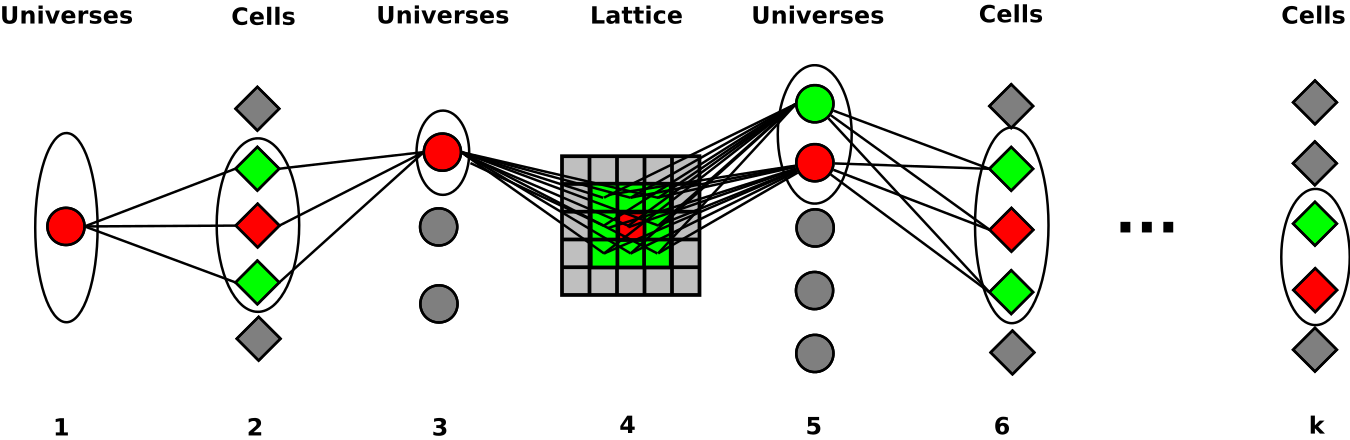
\includegraphics[width=\linewidth]{figures/workflow/opencg/neighbors-k-partite-graph}
  \caption[A $k$-partite graph created by the OpenCG LNS algorithm]{An example $k$-partite graph structure used to identify local neighbor symmetries. Red nodes correspond to the universes/cells encapsulating a region of interest, green nodes correspond to the neighbors of that region, and gray nodes correspond to universes/cells which are not neighbors. Red and green nodes at each level are combined into an argument for a hash function to generate a \ac{LNS} ID for the region of interest.}
  \label{fig:lns-k-partite-graph}
\end{figure}

Several parameters are incorporated into OpenCG's \ac{LNS} \ac{API} to provide the user with various methods to adjust the number of symmetries discovered by the algorithm. For example, OpenCG includes \textit{general} and \textit{unique} neighbor identifiers. General neighbors includes all neighbor cells/universes found by \ac{BFS} -- including duplicates -- as separate nodes in the $k$-partite graph. For example, a single universe may be placed multiple times around a lattice cell, each instance of which will be independently discovered by \ac{BFS} and replicated as a distinct node within the graph. On the contrary, unique neighbors does not include duplicate cells/universes -- only unique cells/universes are represented by distinct nodes in each independent set in the $k$-partite graph. A few diagrams of general and unique \ac{LNS} applied to two geometries are depicted in Fig.~\ref{fig:neighbor-cells}.

\begin{figure}[h!]
\begin{subfigure}{.5\textwidth}
  \centering
  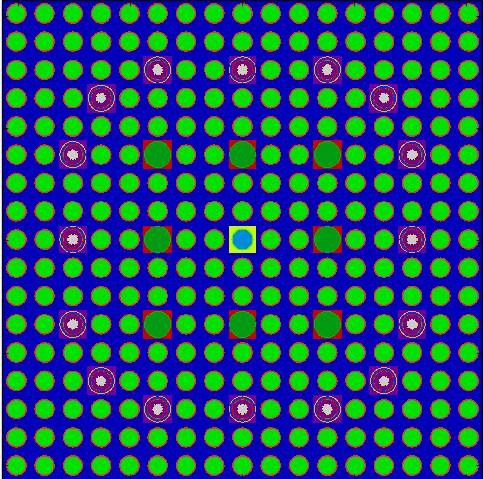
\includegraphics[width=.7\linewidth]{figures/workflow/opencg/cells-xy-24-16-assm}
  \caption{}
  \label{fig:assm-cells}
\end{subfigure}%
\begin{subfigure}{.5\textwidth}
  \centering
  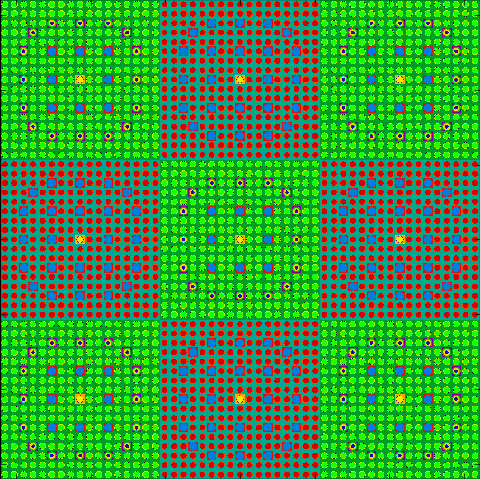
\includegraphics[width=.7\linewidth]{figures/workflow/opencg/cells-xy-colorset}
  \caption{}
  \label{fig:colorset-cells}
\end{subfigure}
\begin{subfigure}{.5\textwidth}
  \centering
  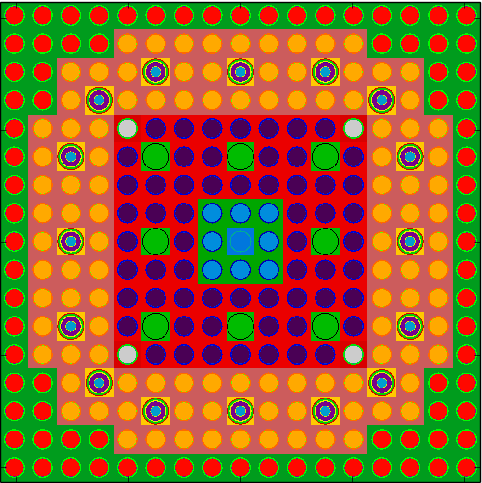
\includegraphics[width=.7\linewidth]{figures/workflow/opencg/unique-neighbor-cells-xy-24-16-assm}
  \caption{}
  \label{fig:assm-unique-neighbors}
\end{subfigure}
\begin{subfigure}{.5\textwidth}
  \centering
  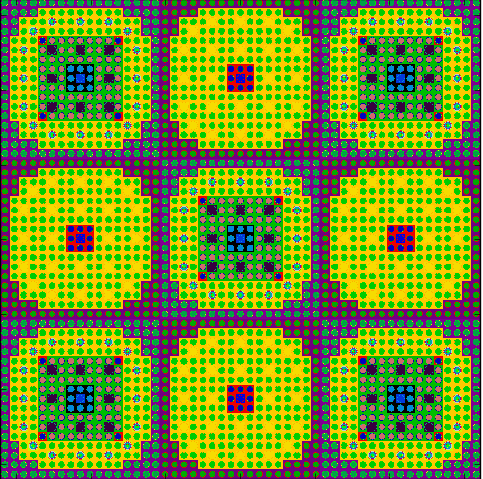
\includegraphics[width=.7\linewidth]{figures/workflow/opencg/unique-neighbor-cells-xy-colorset}
  \caption{}
  \label{fig:colorset-unique-neighbors}
\end{subfigure}
\begin{subfigure}{.5\textwidth}
  \centering
  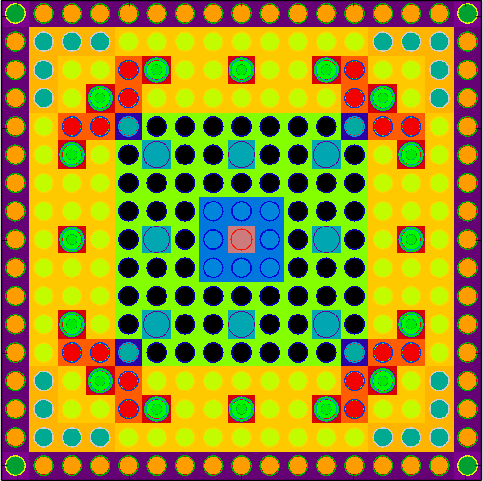
\includegraphics[width=.7\linewidth]{figures/workflow/opencg/neighbor-cells-xy-24-16-assm}
  \caption{}
  \label{fig:assm-neighbors}
\end{subfigure}
\begin{subfigure}{.5\textwidth}
  \centering
  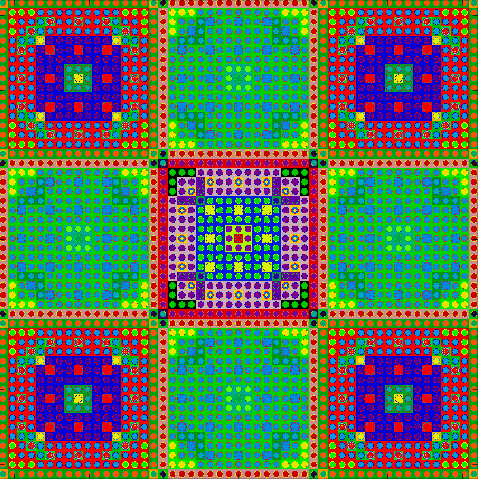
\includegraphics[width=.7\linewidth]{figures/workflow/opencg/neighbor-cells-xy-colorset}
  \caption{}
  \label{fig:colorset-neighbors}
\end{subfigure}
\caption[Example OpenCG Local Neighbor Symmetry mappings]{Two rectilinear lattice geometries are depicted to illustrate the use of local neighbor symmetry identification~\cite{boyd2015opencg}. The \textit{cells} are depicted for (a) a 17$\times$17 PWR lattice and (b) a 3$\times$3 colorset of two different 17 $\times$ 17 PWR assemblies each with burnable absorbers, guide tubes and instrument tubes. The \textit{unique neighbor} symmetry identifiers are color-coded in (b) and (c) for the assembly and colorset, respectively. Likewise, the \textit{general neighbor} symmetry identifiers are color-coded in (d) and (f).}
\label{fig:neighbor-cells}
\end{figure}

To this author's knowledge there is no other implementation of \ac{LNS} aside from that in the OpenCG code. The \ac{LNS} algorithm was used extensively in this thesis as a deterministic ``clustering'' technique for the spatial homogenization methodology introduced in Chaps.~\Crefrange{chap:benchmarks}{chap:unsupervised}. In particular, \ac{LNS} was used to predict which fuel pins have similar \ac{MGXS} in \ac{LWRs} due to spatial self-shielding effects induced by neighboring fuel, guide tube and absorber pins. The \ac{LNS} scheme served as a proxy to the traditional geometric template approach used in lattice physics codes to group pins with like \ac{MGXS}. The spatial homogenization methodology developed in Chaps.~\Crefrange{chap:benchmarks}{chap:unsupervised} incorporates \ac{MC} tally data in unsupervised clustering in an attempt to outperform \ac{LNS}' analysis based solely on the geometry.


%%%%%%%%%%%%%%%%%%%%%%%%%%%%%%%%%%%%
\subsection{Region Differentiation}
\label{sec:chap4-region-diff}

As previously noted, one of the advantages of combinatorial geometry is that it can take advantage of patterned structures with repeating primitives. In certain use cases, however, it may be necessary to replicate certain primitives which have the same geometric properties but experience very different radiation and/or thermal hydraulic conditions, and hence have different material properties in a transport simulation. For example, the \ac{LNS} algorithm is useful for identifying groups of fuel pin cell instances which may have similar \ac{MGXS}. However, in order for a transport code to make use of \ac{LNS}, a replica of each cell must be made to represent each of its different \ac{LNS} identifiers.

%first paragraph: motivation
%-build combinatorial geometries based on arbitrary clustering of cell instances

The process of manually constructing a \ac{CG} with many replicated but geometrically identical cells is very time consuming and prone to errors. To address this issue, a novel algorithm termed \textit{region differentiation} was implemented in OpenCG to efficiently and systematically reconstruct a \ac{CG} with replicated cells~\cite{boyd2015opencg}. A characterization of the region differentiation algorithm applied to a \ac{CG} tree data structure is shown in Fig.~\ref{fig:region-differentiation}.

The region differentiation algorithm is implemented in OpenCG and presents an interface which takes in a set of arbitrarily formed \textit{region groupings}. A region grouping is the set of all regions, that reference a particular cell in the geometry. Alternatively, a region grouping can be thought of as a set of repeated instances of a cell throughout a combinatorial geometry. Two or more region groupings corresponding to the same cell designate specific cell instances that should be replicated. The region differentiation algorithm replicates cells, universes, and lattices for each region grouping.

A naive or brute-force implementation of the region differentiation algorithm would scale as $\mathcal{O}(kn!)$ in both memory and time for $k$ nested universe/cell levels and $n$ region groupings. The reason is that \textit{a priori}, the algorithm does not know from which region groupings various cell instances will combine with one another to form universes, lattices and/or cells, which must themselves be differentiated for each possible combination of region groupings. To avoid factorial scaling, OpenCG makes use of dynamic programming to efficiently differentiate primitives one level at a time within the geometry.

\afterpage{\clearpage}
\begin{figure}[p]
\begin{subfigure}{\textwidth}
  \centering
  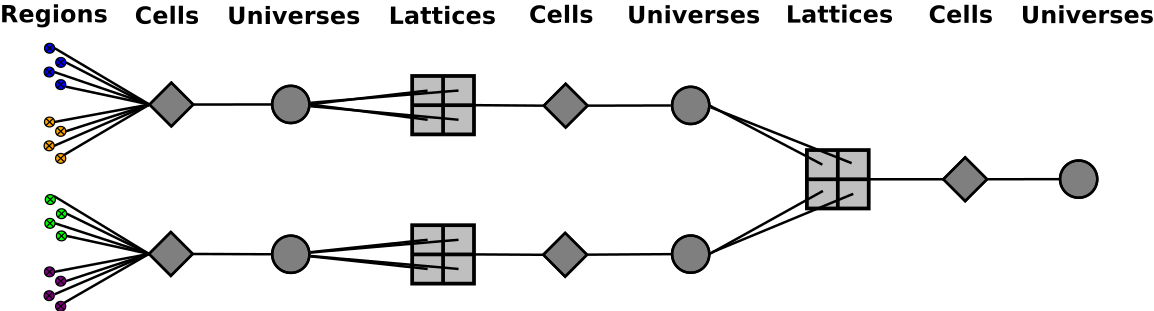
\includegraphics[width=0.82\linewidth]{figures/workflow/opencg/region-differentiation-1}
  \caption{}
  \label{fig:differentation-1}
\end{subfigure}
\begin{subfigure}{\textwidth}
  \centering
  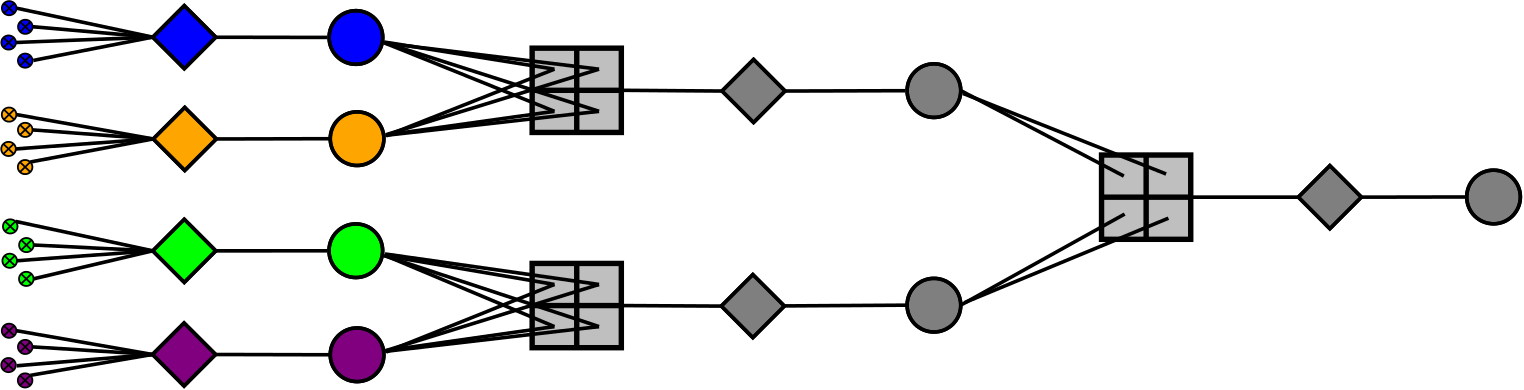
\includegraphics[width=0.75\linewidth]{figures/workflow/opencg/region-differentiation-2}
  \caption{}
  \label{fig:differentation-2}
\end{subfigure}
\begin{subfigure}{\textwidth}
  \centering
  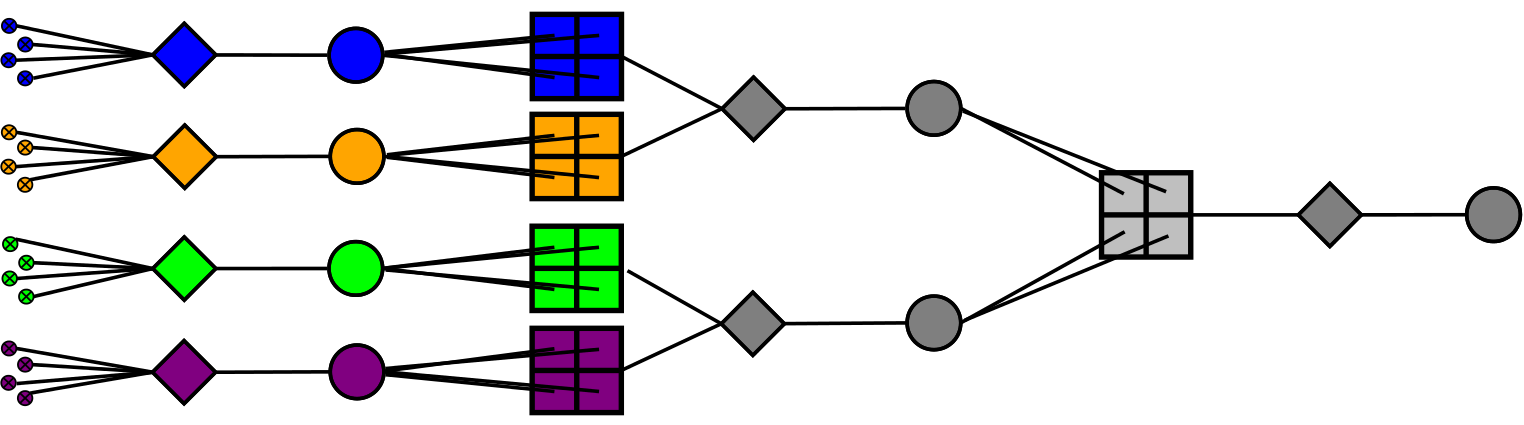
\includegraphics[width=0.75\linewidth]{figures/workflow/opencg/region-differentiation-3}
  \caption{}
  \label{fig:differentation-3}
\end{subfigure}
\begin{subfigure}{\textwidth}
  \centering
  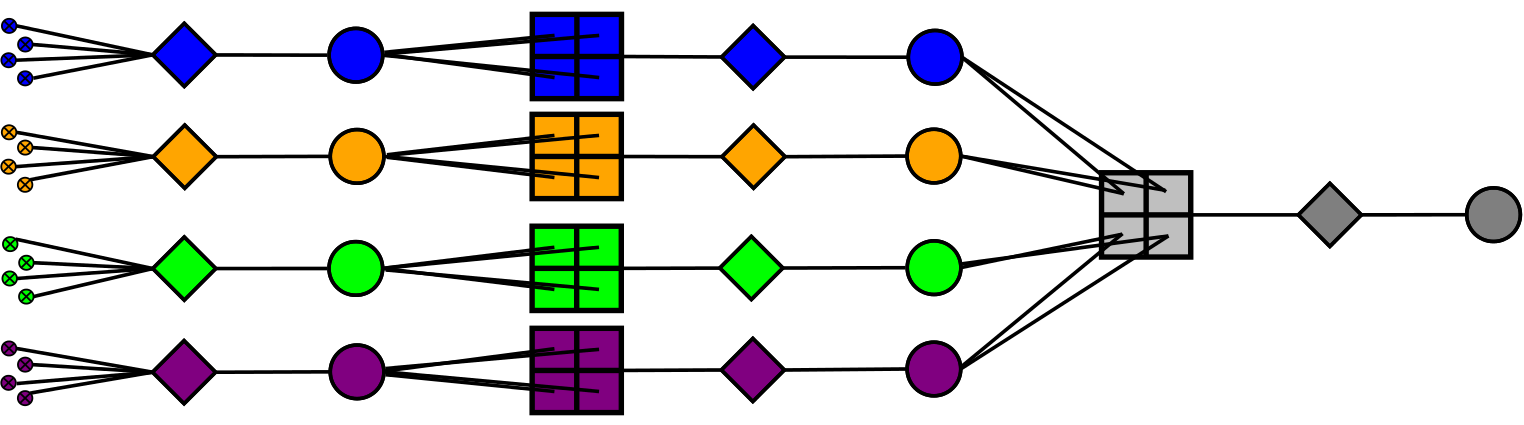
\includegraphics[width=0.75\linewidth]{figures/workflow/opencg/region-differentiation-4}
  \caption{}
  \label{fig:differentation-4}
\end{subfigure}
\begin{subfigure}{\textwidth}
  \centering
  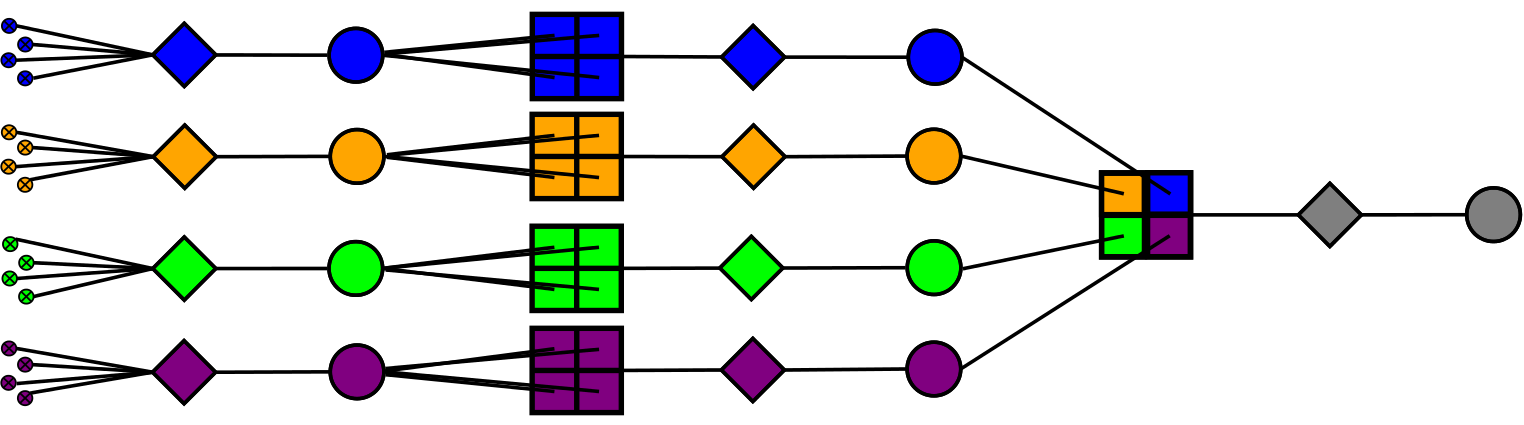
\includegraphics[width=0.75\linewidth]{figures/workflow/opencg/region-differentiation-5}
  \caption{}
  \label{fig:differentation-5}
\end{subfigure}
\caption[A few stages of the OpenCG region differentiation algorithm]{A few of the stages of the region differentiation algorithm~\cite{boyd2015opencg}. The regions (cell instances) to be differentiated are grouped and colored blue, orange, green and purple in (a). The first levels of cells and universes for each region group are differentiated in (b). The same is done for the lattices in (c). The algorithm continues to recursively differentiate cells, universes and lattices until no region groups collide at any level of the CG tree in (e).}
\label{fig:region-differentiation}
\end{figure}

The region differentiation algorithm iterates over each level of nested universes and cells. At each step, the paths for each region starting from the current level in the \ac{CG} tree and ending with the root universe node are hashed and stored in a hash table linked to the region grouping. Next, the algorithm manages \textit{primitive collisions} when two or more region groupings with the same path in the hash table point to the same primitive (cell, universe or lattice). To resolve primitive collisions, the algorithm differentiates the primitive for each region grouping involved in the collision. As primitive collisions are resolved, the algorithm merges any region groupings with paths that hash to same value in the hash table. The algorithm's termination condition is reached when the hash table only has one entry -- \textit{i.e.}, paths for all regions hash to the same value.

The region differentiation algorithm was an indispensable component of the simulation triad used to explore novel \ac{MGXS} generation techniques in this thesis. In particular, region differentiation made it possible to rapidly construct geometries to reflect the assignment of \ac{MGXS} to arbitrary collections of fuel pins for the spatial homogenization methodology introduced in Chaps.~\Crefrange{chap:benchmarks}{chap:unsupervised}. Fig.~\ref{fig:region-diff-proc-diagram} illustrates a flow diagram where the \ac{LNS} algorithm identifies the region groupings input to the region differentiation algorithm. The geometry produced from region differentiation may then be exported for use in OpenMC or OpenMOC using the compatibility modules discussed in Sec.~\ref{sec:chap4-opencg-compatibility}.

\begin{figure}[h!]
  \centering
  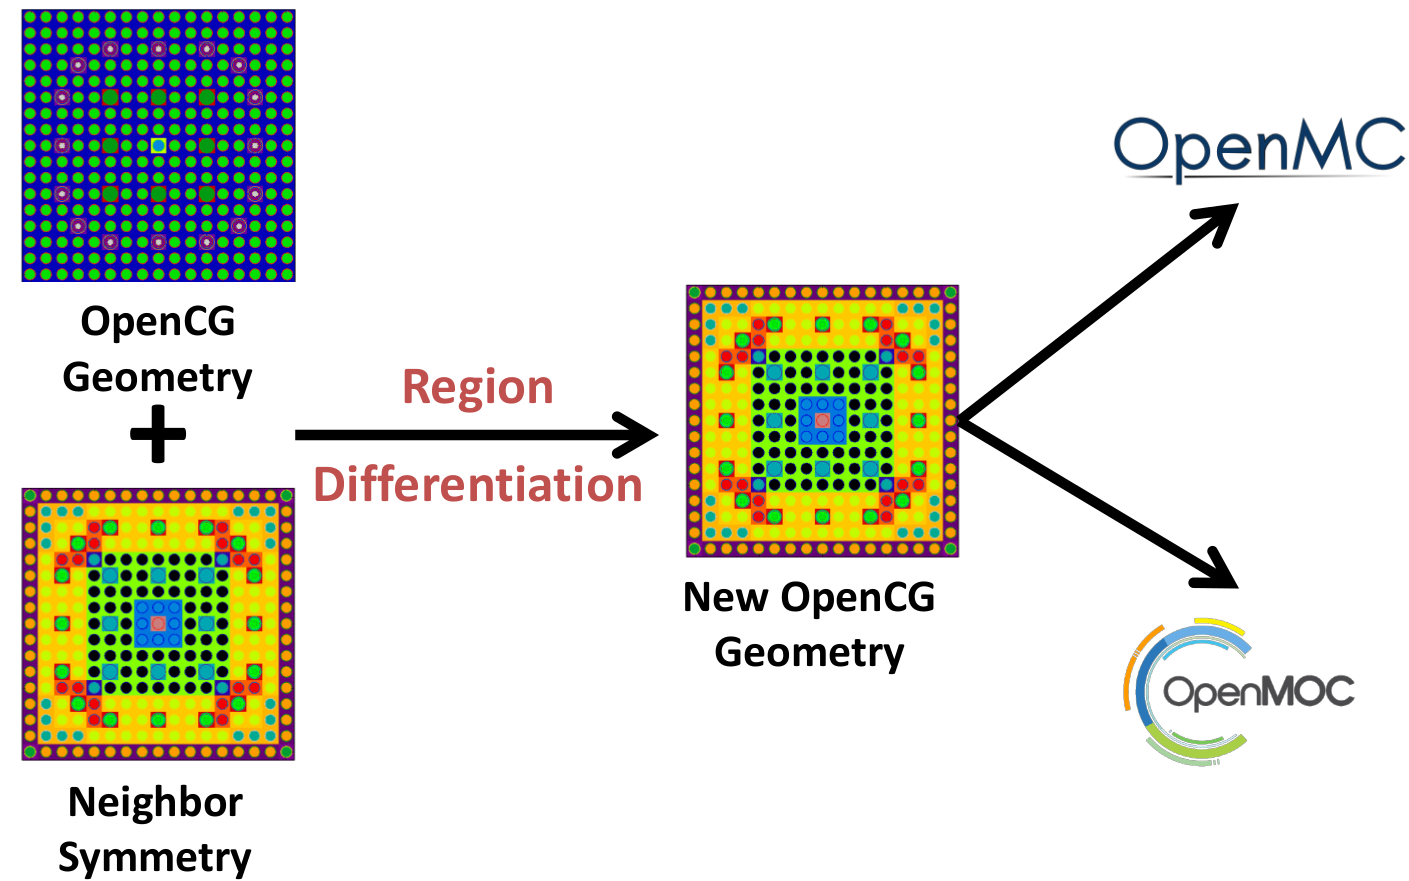
\includegraphics[width=0.8\linewidth]{figures/workflow/opencg/region-diff-proc-diagram}
  \caption[OpenCG region differentiation process diagram]{The OpenCG \ac{LNS} algorithm may be used to generate region groupings for the region differentiation algorithm to create a geometry for OpenMC or OpenMOC.}
  \label{fig:region-diff-proc-diagram}
\end{figure}

\begin{emphbox}
\textbf{The OpenCG code was implemented to facilitate data transfer between OpenMC and OpenMOC. The \ac{LNS} and region differentiation algorithms supported the novel spatial homogenization methodology developed in Chaps.~\Crefrange{chap:benchmarks}{chap:unsupervised}.}
\end{emphbox}


\vfill
\begin{highlightsbox}[frametitle=Highlights]
\begin{itemize}
  \item A framework consisting of the OpenMC, OpenMOC and OpenCG codes comprise a ``simulation triad'' used to explore \ac{MC}-based \ac{MGXS} generation methods for fine mesh transport calculations.
  \item A fully-featured Python \ac{API} was developed to support input generation and downstream processing of large tally datasets for OpenMC.
  \item The \texttt{openmc.mgxs} Python module was created to generate \ac{MGXS} from OpenMC tallies. The distributed cell tally algorithm was implemented to generate pin-wise \ac{MGXS} in large, heterogeneous geometries.
  \item New features were added to the deterministic multi-group OpenMOC code to enable it to use \ac{MGXS} generated by \texttt{openmc.mgxs} in 2D \ac{MOC} calculations.
  \item The OpenCG code was created to facilitate data processing and transfer on the combinatorial geometry meshes used by OpenMC and OpenMOC.
  \item OpenCG's \ac{LNS} and region differentiation algorithms were crucial components for the spatial homogenization methodology developed in Chaps.~\Crefrange{chap:benchmarks}{chap:unsupervised}.  
\end{itemize}
\end{highlightsbox}
\vfill

\part{Approximation Error}
\chapter{Quantifying MGXS Approximations}
\label{chap:biases}

As discussed in Chapter~\ref{chap:mgxs}, a number of approximations are made in the multi-group formulation of the neutron transport equation and the \ac{MGXS} generation process. These approximations remain even if one uses the ``true'' scalar flux for energy condensation and spatial homogenization, as is the case with energy condensation and spatial homogenization in Monte Carlo\footnote{By the Law of Large Numbers, the \ac{MC} flux will be exactly correct in the limit of an infinite number of particle histories, though it is only a ``noisy'' proxy for a finite number of particles.}. The observed bias between a continuous energy \ac{MC} and a multi-group deterministic calculation reflects the convolution of these approximations, which may (or may not) lead to some degree of fortuitous cancellation of error. Although this thesis is motivated by the need for \ac{MGXS} for whole-core calculations, it is instructive to investigate the approximations inherent in multi-group theory and quantify their impact for simple benchmark models.

In this chapter, a series of case studies is devised to systematically quantify biases inherent to the energy condensation and spatial homogenization process(es) in multi-group transport theory. The results underline the complex interactions between discretizations in energy, space and angle. Various convergence studies with respect to each of these variables are presented to quantify the resulting magnitude of the bias induced between continuous energy Monte Carlo and multi-group deterministic calculations. The results in this chapter illustrate the loss in accuracy resulting from scalar flux-weighted total \ac{MGXS} due to the flux separability approximation (see Sec.~\ref{subsec:chap2-angle}), and highlight the need for models of the angular dependency in \ac{MGXS} for fine mesh deterministic neutron transport. Finally, this chapter verifies the data pipeline used to compute multi-group cross sections with OpenMC for use in OpenMOC (see Chap.~\ref{chap:workflow}).


%%%%%%%%%%%%%%%%%%%%%%%%%%%%%%%%%%%%%%%%%%%%%%%%%%%%%%%%%%%%%%%%%%%%%%%%%%%%%%%%
\section{Case Studies}
\label{sec:chap5-case-studies}

This chapter investigates the loss in accuracy resulting from approximations made in both the \ac{MOC} equations as well as the \ac{MGXS} generation scheme with OpenMC. The benchmarks are designed to illustrate the emergence of the approximation errors as spatial heterogeneity is introduced in the geometric models. The approximation errors are quantified for a variety of geometric and material configurations based on a standard \ac{PWR}. In each case, the bias $\Delta\rho$ compares the eigenvalue $k_{eff}^{OpenMOC}$ computed with \ac{MGXS} in OpenMOC to that of the reference eigenvalue $k_{eff}^{OpenMC}$ computed with continuous energy cross sections in OpenMC in units of \ac{pcm}:

\begin{equation}
\label{eqn:chap5-delta-rho}
\Delta\rho = \left(k_{eff}^{OpenMOC} - k_{eff}^{OpenMC}\right) \times 10_{5}
\end{equation}

In each case study, the role of angular discretization in \ac{MOC} is quantified through convergence studies of the number of azimuthal angles and the track spacing used in the deterministic \ac{MOC} calculations. The effects of energy discretization are analyzed for \ac{MGXS} tallied in the CASMO~\cite{rhodes2006casmo} energy group structures ranging from 1 -- 70 groups (see App.~\ref{app:energy-groups}). For each of the case studies with heterogeneous geometries, the spatial domain is discretized in OpenMOC's \ac{FSR} mesh with constant-by-material \ac{MGXS} to quantify the interaction between the energy and spatial approximations. Spatial discretization studies show the impact of tallying \ac{MGXS} in each of the \ac{FSR}s used in the discretized OpenMOC geometry. Finally, \ac{MGXS} libraries were tallied using OpenMC's iso-in-lab feature (see Sec.~\ref{subsec:chap4-iso-in-lab}) to quantify the impact of the isotropic in lab scattering approximation used in OpenMOC. Inter-pin spatial self-shielding effects are not treated here as they are studied in detail in Chaps.~\Crefrange{chap:benchmarks}{chap:unsupervised}. In each case study, OpenMOC was converged to a criterion of 10$^{-7}$ on the root mean square of the energy-integrated fission source in each \ac{FSR}.

%%%%%%%%%%%%%%%%%%%%%%%%%%%%
\subsection{Homogeneous Infinite Medium}
\label{subsec:chap5-inf-medium}

An initial series of case studies were performed for a homogeneous infinite medium problem. The isotopic composition of the infinite medium was a homogenized mixture derived from the 1.6\% enriched UO$_2$ \ac{PWR} fuel pin in the \ac{BEAVRS} \ac{PWR} model~\cite{horelik2013beavrs} and is described in Tab.~\ref{table:chap5-inf-med-isotopes}. No approximation is made in the multi-group formulation of the transport equation in the case of homogeneous infinite media. As a result, neutron balance should be exactly preserved within numerical precision in deterministic calculations with \ac{MGXS} computed in any energy group structure, assuming the \ac{MC} tallies used to compute \ac{MGXS} are sufficiently converged.

\begin{table}[h!]
  \centering
  \caption[Infinite medium isotopic composition]{Homogeneous infinite medium isotopic composition.}
  \small
  \label{table:chap5-inf-med-isotopes} 
  \vspace{6pt}
  \begin{tabular}{c c}
  \toprule
  \rowcolor{lightgray}
  {\bf Nuclide} &
  {\bf Density [atoms / b-cm]} \\
  \midrule
  H-1 &   4.12377E-2 \\
  O-16 &  2.06218E-2 \\
  Zr-90 & 3.00904E-3 \\
  U-235 & 1.62310E-4 \\
  U-238 & 9.79198E-3 \\
  \bottomrule
\end{tabular}
\end{table}

The reference eigenvalues computed with continuous energy cross sections in OpenMC are shown in Tab.~\ref{table:chap5-inf-med-reference} for both normal anisotropic as well as iso-in-lab scattering. As one would expect for a homogeneous infinite medium, the eigenvalues for anisotropic and iso-in-lab scattering agree to within one standard deviation of the mean. The reference calculations were computed for 100 batches of 10$^{8}$ particles per batch. The \texttt{openmc.mgxs} module was used to compute 70-group libraries of $\hat{\Sigma}_{t,g}$, $\hat{\Sigma}_{s,k,g'\rightarrow g}$, $\nu\hat{\Sigma}_{f,g}$, and $\hat{\chi}_{g}$ from OpenMC tallies (see Tab.~\ref{table:chap3-tally-types}).

\begin{table}[h!]
  \centering
  \caption[Reference $k^{OpenMC}_{\infty}$ for an infinite medium]{Reference $k^{OpenMC}_{\infty}$ for a homogeneous infinite medium.}
  \small
  \label{table:chap5-inf-med-reference} 
  \vspace{6pt}
  \begin{tabular}{c c}
  \toprule
  \rowcolor{lightgray}
  {\cellcolor{carolinablue} {\bf Anisotropic}} &
  {\cellcolor{lightgreen} {\bf Isotropic in Lab}} \\
  \midrule
  1.15908 $\pm$ 0.00001 & 1.15907 $\pm$ 0.00001 \\
  \bottomrule
\end{tabular}
\end{table}

%%%%%%%%%%%%%%%%%%%%%%%%%%%%%%%%%%%%%%%%%%%%%%%
\subsubsection{Angular Discretization}
\label{subsubsec:chap5-inf-med-angle}

The first case study investigated the sensitivity of the OpenMOC eigenvalue to the angular discretization used in the \ac{MOC} calculation. Tab.~\ref{table:chap5-inf-med-angle} presents the bias $\Delta\rho$ between OpenMC and OpenMOC for a matrix of azimuthal angles and track spacings. The results for both normal and iso-in-lab scattering indicate consistent agreement of the eigenvalues irregardless of track discretization. This result is expected since the neutron source is isotropic in homogeneous infinite media and does not depend on the angular discretization used to solve the eigenvalue problem.

\vspace{0.1in}

\begin{table}[h!]
  \centering
  \caption[Angular discretization error for an infinite medium]{Convergence study of the eigenvalue bias $\Delta\rho$ with varying azimuthal angle quadratures and track spacings for a homogeneous infinite medium.}
  \small
  \label{table:chap5-inf-med-angle}
  \vspace{6pt}
  \begin{tabular}{| q | S[table-format=4.1] S[table-format=4.1] S[table-format=4.1] | S[table-format=4.1] S[table-format=4.1] S[table-format=4.1] |}
  \hhline{~|------|}
  \multicolumn{1}{c|}{} &
  \multicolumn{6}{c|}{\cellcolor{lightgray} \bf Track Spacing [cm]} \\
  \multicolumn{1}{c|}{} &
  {\cellcolor{lightgray} \bf 0.1} &
  {\cellcolor{lightgray} \bf 0.01} & 
  \multicolumn{1}{S[table-format=4.1]}{\cellcolor{lightgray} {\bf 0.001}} &
  \multicolumn{1}{S[table-format=4.1]}{\cellcolor{lightgray} {\bf 0.1}} & 
  {\cellcolor{lightgray} \bf 0.01} & 
  \multicolumn{1}{S[table-format=4.1]|}{\cellcolor{lightgray} {\bf 0.001}} \\
  \midrule
  {\bf \# Angles} & \multicolumn{3}{c|}{\cellcolor{carolinablue} \bf Anisotropic} &
  \multicolumn{3}{c|}{\cellcolor{lightgreen} \bf Isotropic in Lab} \\
  \cline{2-7}
4 & 1.3 & 1.3 & 1.3 & -0.1 & -0.1 & -0.1 \\
8 & 1.3 & 1.3 & 1.3 & -0.1 & -0.1 & -0.1 \\
16 & 1.3 & 1.3 & 1.3 & -0.1 & -0.1 & -0.1 \\
32 & 1.3 & 1.3 & 1.3 & -0.1 & -0.1 & -0.1 \\
64 & 1.3 & 1.3 & 1.3 & -0.1 & -0.1 & -0.1 \\
128 & 1.3 & 1.3 & 1.3 & -0.1 & -0.1 & -0.1 \\
  \bottomrule
\end{tabular}
\end{table}

%%%%%%%%%%%%%%%%%%%%%%%%%%%%%%%%%%%
\subsubsection{Energy Condensation}
\label{subsubsec:chap5-inf-med-energy}

A second case study investigated the variation of the OpenMOC eigenvalue with the energy group structure used in the \ac{MOC} calculation. Tab.~\ref{table:chap5-inf-med-energy} presents the bias $\Delta\rho$ between OpenMC and OpenMOC for a matrix of energy group structures and \ac{FSR} spatial discretizations. The OpenMOC calculations each used 128 azimuthal angles and 0.01 cm track spacing. Although the eigenvalues differ by approximately 10 \ac{pcm} for 1 and 2 groups, the OpenMOC eigenvalues match the eigenvalues computed analytically from the 1- and 2-group \ac{MGXS} to within 1 pcm. The 10 \ac{pcm} bias may be due to numerical roundoff error since the \ac{MGXS} library was tallied in 70 groups in OpenMC and condensed to the coarser group structures with data processing  by the \texttt{openmc.mgxs} module.

\begin{table}[h!]
  \centering
  \caption[Energy discretization error for an infinite medium]{Convergence study of the eigenvalue bias $\Delta\rho$ with varying energy group structures for a homogeneous infinite medium.}
  \small
  \label{table:chap5-inf-med-energy} 
  \vspace{6pt}
  \begin{tabular}{| q | S[table-format=2.1] | S[table-format=2.1] |}
  \toprule
  {\bf \# Groups} &
  {\cellcolor{carolinablue} {\bf \hspace{0.3cm}Anisotropic\hspace{0.3cm}}} &
  {\cellcolor{lightgreen} {\bf Isotropic in Lab}} \\
  \cline{2-3}
1 & -11.1 & -10.5 \\
2 & -9.5 & -7.1 \\
4 & -0.1 & -0.5 \\
8 & 0.3 & -0.0 \\
16 & -0.2 & 0.5 \\
25 & 1.8 & 0.1 \\
40 & 1.6 & 0.1 \\
70 & 1.3 & -0.1 \\
  \bottomrule
\end{tabular}
\end{table}

\vspace{0.5cm}
\begin{emphbox}
\textbf{The eigenvalues for a homogeneous infinite medium agree to within nearly 10 \ac{pcm} for all \ac{MOC} angular discretizations and energy group structures.}
\end{emphbox}


%%%%%%%%%%%%%%%%%%%%
\subsection{1D Slab}
\label{subsec:chap5-slab}

A simple slab model was constructed to quantify approximation errors in a 1D heterogeneous geometry with spatial self-shielding. The slab model was constructed as an ``equivalent'' 1D model to the 2.4\% enriched UO$_2$ \ac{PWR} fuel pin in the \ac{BEAVRS} \ac{PWR} model~\cite{horelik2013beavrs}. The geometric configuration of UO$_2$ fuel, helium gap, zirconium clad and water moderator is illustrated in Fig.~\ref{fig:chap5-slab} and the dimensions for each material zone are shown in Tab.~\ref{table:chap5-slab-widths}. The width of each spatial region was chosen to preserve the volumetric fraction of each material in the slab with those in the corresponding 2D fuel pin\footnote{A truly ``equivalent'' slab would preserve the mean chord lengths of each material in the 2D fuel pin.}. Reflective boundary conditions were applied to all $x$, $y$ and $z$ boundaries in the geometry. The isotopic composition of each material in the slab is identical to the \ac{BEAVRS} fuel pin and is itemized in Tab.~\ref{table:chap5-slab-isotopes}. 

\begin{figure}[h!]
\begin{subfigure}{\textwidth}
  \centering
  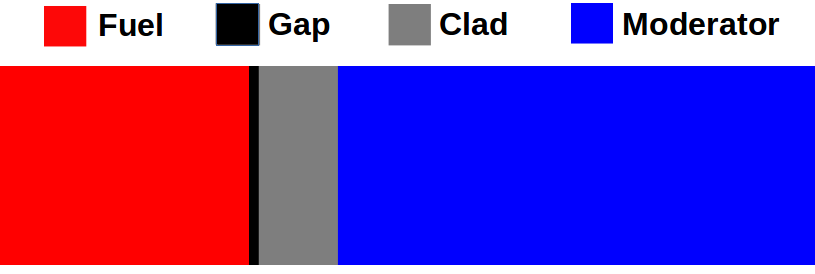
\includegraphics[width=0.7\linewidth]{figures/biases/slab/slab-simple-labels}
  \caption{}
  \label{fig:chap5-slab-a}
\end{subfigure} \\
\begin{subfigure}{\textwidth}
  \centering
  
\includegraphics[width=0.7\linewidth]{figures/biases/slab/slab-8x}
  \caption{}
  \label{fig:chap5-slab-b}
\end{subfigure}
\caption[1D slab materials and geometry]{A 1D slab with fuel, clad and moderator (a). Linearly-spaced tally zones were defined in the fuel and moderator in OpenMC and as \ac{FSR}s in OpenMOC (b).}
\label{fig:chap5-slab}
\end{figure}

\begin{table}[h!]
  \centering
  \caption[1D slab dimensions]{1D slab dimensions.}
  \small
  \label{table:chap5-slab-widths} 
  \vspace{6pt}
  \begin{tabular}{l c}
  \toprule
  \rowcolor{lightgray}
  \multicolumn{1}{c}{\bf Material} &
  \multicolumn{1}{c}{\bf Width [cm]} \\
  \midrule
  Fuel &  0.19177 \\
  Gap &   0.00777 \\
  Clad &  0.06109 \\
  Water & 0.36929 \\
  \bottomrule
\end{tabular}
\end{table}

\begin{table}[h!]
  \centering
  \caption[1D slab isotopic composition]{1D slab isotopic composition.}
  \small
  \label{table:chap5-slab-isotopes} 
  \vspace{6pt}
  \begin{tabular}{c c c}
  \toprule
  \rowcolor{lightgray}
  {\bf Material} &
  {\bf Nuclide} &
  {\bf Density [atoms / b-cm]} \\
  \midrule
  \multirow{3}{*}{\bf UO$_2$} & O-16 &  4.58508E-2 \\
  & U-235 & 5.58415E-4 \\
  & U-238 & 2.24186E-2 \\
  \midrule
  \multirow{1}{*}{\bf Helium} & He-4 & 2.40428E-4 \\
  \midrule
  \multirow{3}{*}{\bf Zircaloy} & O-16 &  6.14041E-4 \\
  & Fe-56 & 2.71837E-4 \\
  & Zr-90 & 4.35958E-2 \\
  \midrule
  \multirow{4}{*}{\bf Water} & H-1 &  4.95774E-2 \\
  & B-10 & 8.02369E-6 \\
  & B-11 & 3.22964E-5 \\
  & O-16 & 2.47320E-2 \\
  \bottomrule
\end{tabular}
\end{table}

The reference eigenvalues computed with continuous energy cross sections in OpenMC are shown in Tab.~\ref{table:chap5-slab-reference} for both normal anisotropic as well as iso-in-lab scattering. The reference calculations were computed for 100 batches of 10$^{7}$ particles per batch. The reference eigenvalues for the two cases vary by nearly 75 \ac{pcm} due to anisotropies resulting from thermal scattering in the moderator. The \texttt{openmc.mgxs} module was used to compute 70-group libraries of $\hat{\Sigma}_{t,k,g}$, $\hat{\tilde{\Sigma}}_{t,k,g}$, $\hat{\Sigma}_{s,k,g'\rightarrow g}$, $\hat{\tilde{\Sigma}}_{s,k,g'\rightarrow g}$, $\nu\hat{\Sigma}_{f,g}$, and $\hat{\chi}_{g}$ from OpenMC tallies (see Tab.~\ref{table:chap3-tally-types}).

\begin{table}[h!]
  \centering
  \caption[Reference $k^{OpenMC}_{eff}$ for a 1D slab]{Reference $k^{OpenMC}_{eff}$ for a 1D slab.}
  \small
  \label{table:chap5-slab-reference} 
  \vspace{6pt}
  \begin{tabular}{c c}
  \toprule
  \rowcolor{lightgray}
  {\cellcolor{carolinablue} {\bf Anisotropic}} &
  {\cellcolor{lightgreen} {\bf Isotropic in Lab}} \\
  \midrule
  1.16275 $\pm$ 0.00003 & 1.16202 $\pm$ 0.00003 \\
  \bottomrule
\end{tabular}
\end{table}

%%%%%%%%%%%%%%%%%%%%%%%%%%%%%%%%%%%%%%%%%%%%%%%
\subsubsection{Angular Discretization}
\label{subsubsec:chap5-slab-angle}

The first case study investigated the convergence of the OpenMOC eigenvalue with the angular discretization used in the \ac{MOC} calculation. Tab.~\ref{table:chap5-slab-angle} presents the bias $\Delta\rho$ between OpenMC and OpenMOC for a matrix of azimuthal angles and track spacings. Two different 70-group \ac{MGXS} libraries were computed from OpenMC tallies with anisotropic and iso-in-lab scattering. No transport correction was applied to the total cross section $\hat{\Sigma}_{t,k,g}$ or the scattering matrix $\hat{\Sigma}_{s,k,g'\rightarrow g}$. No spatial discretization was applied to the materials for the \ac{FSR} mesh in OpenMOC. The results for anisotropic and iso-in-lab scattering exhibit a bias resulting from the multi-group approximation which converges to 170 and 280 pcm, respectively. The magnitude of the bias appears to converge with 128 azimuthal angles and was largely insensitive to the track spacing. The \ac{MGXS} tallied with iso-in-lab scattering in OpenMC eliminates the isotropic scattering approximation in OpenMOC but increases the overall bias by over 100 \ac{pcm} with respect to the anisotropic case due to the cancellation of other approximation errors.

\begin{table}[h!]
  \centering
  \caption[Angular discretization error for a 1D slab]{Convergence study of the 70-group eigenvalue bias $\Delta\rho$ with varying azimuthal angle quadratures and track spacings for a 1D slab.}
  \small
  \label{table:chap5-slab-angle}
  \vspace{6pt}
  \begin{tabular}{| q | S[table-format=6.1] S[table-format=6.1] S[table-format=6.1] | S[table-format=6.1] S[table-format=6.1] S[table-format=6.1] |}
  \hhline{~|------|}
  \multicolumn{1}{c|}{} &
  \multicolumn{6}{c|}{\cellcolor{lightgray} \bf Track Spacing [cm]} \\
  \multicolumn{1}{c|}{} &
  {\cellcolor{lightgray} \bf 0.1} &
  {\cellcolor{lightgray} \bf 0.01} & 
  \multicolumn{1}{S[table-format=6.1]}{\cellcolor{lightgray} {\bf 0.001}} &
  \multicolumn{1}{S[table-format=6.1]}{\cellcolor{lightgray} {\bf 0.1}} & 
  {\cellcolor{lightgray} \bf 0.01} & 
  \multicolumn{1}{S[table-format=6.1]|}{\cellcolor{lightgray} {\bf 0.001}} \\
  \midrule
  {\bf \# Angles} & \multicolumn{3}{c|}{\cellcolor{carolinablue} \bf Anisotropic} &
  \multicolumn{3}{c|}{\cellcolor{lightgreen} \bf Isotropic in Lab} \\
  \cline{2-7}
4 & 731 & 731 & 731 & 840 & 840 & 840 \\
8 & 472 & 339 & 323 & 581 & 448 & 432 \\
16 & 282 & 166 & 149 & 390 & 275 & 257 \\
32 & 154 & 135 & 131 & 262 & 243 & 239 \\
64 & 158 & 146 & 156 & 266 & 254 & 265 \\
128 & 165 & 164 & 169 & 274 & 272 & 278 \\
256 & 161 & 171 & 172 & 270 & 280 & 280 \\
512 & 165 & 170 & 172 & 274 & 278 & 281 \\
  \bottomrule
\end{tabular}
\end{table}

\newpage

%%%%%%%%%%%%%%%%%%%%%%%%%%%%%%%%%%%
\subsubsection{Energy Condensation and FSR Discretization}
\label{subsubsec:chap5-slab-energy}

The second case study investigated the variation of the OpenMOC eigenvalue with the energy group structure used in the \ac{MOC} calculation. This case study simultaneously varied the \ac{FSR} discretization used in the OpenMOC simulation. The fuel and moderator were modeled with 1 -- 16 equal volume \ac{FSR}s in each material. The gap and clad were each modeled with a single \ac{FSR}. Tab.~\ref{table:chap5-slab-energy} presents the bias $\Delta\rho$ between OpenMC and OpenMOC for a matrix of energy group structures and \ac{FSR} spatial discretizations. In each case, the \ac{MGXS} used in OpenMOC were tallied by material rather than \ac{FSR} in OpenMC (\textit{i.e.}, the spatial tally mesh corresponded to Fig.~\ref{fig:chap5-slab-a}). The OpenMOC calculations each used 128 azimuthal angles and 0.01 cm track spacing. The slab was discretized into 1 -- 16 equal volume \ac{FSR}s in the fuel and moderator.

\begin{table}[h!]
  \centering
  \caption[Energy and spatial discretization error for a 1D slab]{Convergence study of the eigenvalue bias $\Delta\rho$ with varying energy group structures and \ac{FSR} spatial discretizations for a 1D slab with \textit{\ac{MGXS} tallied by material}.}
  \small
  \label{table:chap5-slab-energy} 
  \vspace{6pt}
  \begin{tabular}{| q | S[table-format=6.1] S[table-format=6.1] S[table-format=6.1] S[table-format=6.1] S[table-format=6.1] |}
  \hhline{~|-----|}
  \multicolumn{1}{c|}{\cellcolor{white}} & \multicolumn{5}{c|}{\cellcolor{lightgray} {\bf \ac{FSR} Discretization}} \\
  \multicolumn{1}{c|}{\cellcolor{white}} &
  {\cellcolor{lightgray} {\bf 1$\times$}} &
  {\cellcolor{lightgray} {\bf 2$\times$}} &
  {\cellcolor{lightgray} {\bf 4$\times$}} &
  {\cellcolor{lightgray} {\bf 8$\times$}} &
  {\cellcolor{lightgray} {\bf 16$\times$}} \\
  \midrule
  \multicolumn{1}{|c|}{\cellcolor{lightgray} {\bf \# Groups}} & \multicolumn{5}{c|}{\cellcolor{carolinablue} \bf Anisotropic w/o Transport Correction} \\
  \hhline{~|-----|}
1 & 70 & 71 & 72 & 72 & 71 \\
2 & 106 & -16 & -80 & -101 & -85 \\
4 & 112 & -2 & -63 & -90 & -87 \\
8 & 158 & -13 & -109 & -149 & -160 \\
16 & 182 & -9 & -117 & -162 & -173 \\
25 & 146 & -37 & -143 & -190 & -201 \\
40 & 155 & -40 & -155 & -205 & -217 \\
70 & 164 & -38 & -156 & -208 & {\cellcolor{darktangerine}} -221 \\
  \midrule
  \multicolumn{1}{c|}{\cellcolor{white}} & \multicolumn{5}{c|}{\cellcolor{lightgreen} \bf Anisotropic w/ Transport Correction} \\
  \midrule
1 & 87 & 88 & 88 & 88 & 87 \\
2 & 285 & 211 & 175 & 167 & 189 \\
4 & 188 & 113 & 75 & 51 & 63 \\
8 & 211 & 81 & 13 & -23 & -24 \\
16 & 232 & 82 & 1 & -39 & -40 \\
25 & 148 & -1 & -89 & -123 & -128 \\
40 & 148 & -14 & -111 & -149 & -156 \\
70 & 153 & -16 & -118 & -158 & {\cellcolor{darktangerine}} -166 \\
  \midrule
  \multicolumn{1}{c|}{\cellcolor{white}} & \multicolumn{5}{c|}{\cellcolor{lightsalmonpink} \bf Isotropic in Lab} \\
  \midrule
1 & 132 & 134 & 135 & 135 & 133 \\
2 & 289 & 167 & 102 & 81 & 97 \\
4 & 226 & 112 & 50 & 24 & 26 \\
8 & 296 & 126 & 30 & -10 & -21 \\
16 & 321 & 131 & 22 & -22 & -33 \\
25 & 258 & 75 & -31 & -78 & -88 \\
40 & 262 & 67 & -47 & -98 & -110 \\
70 & 272 & 71 & -48 & -100 & {\cellcolor{darktangerine}} -113 \\
  \bottomrule
\end{tabular}
\end{table}

The results illustrate a strong interaction between the energy and spatial meshes used to solve the multi-group transport equation. The eigenvalue bias varies by up to 150 \ac{pcm} between energy group structures and nearly 400 \ac{pcm} between \ac{FSR} discretizations. The application of the transport correction reduces the bias by 55 \ac{pcm} for the 70-group structure and 16$\times$ \ac{FSR} discretization. The use of the iso-in-lab scattering feature reduces the bias by an additional 50 \ac{pcm} with respect to anisotropic scattering. 

\clearpage

%%%%%%%%%%%%%%%%%%%%%%%%%%%%%%%%%%%
\subsubsection{Spatial Homogenization and FSR Discretization}
\label{subsubsec:chap5-slab-space}

Finally, a case study was performed to investigate the sensitivity of the OpenMOC eigenvalue to the spatial tally mesh used to compute \ac{MGXS}. This study was identical to that presented in Sec.~\ref{subsubsec:chap5-slab-energy}, but the \textbf{\ac{MGXS} were computed using a tally mesh in OpenMC identical to the \ac{FSR} mesh used by OpenMOC}. Tab.~\ref{table:chap5-slab-space} presents the bias $\Delta\rho$ for a matrix of energy group structures and \ac{MGXS} spatial tally zone meshes. In each case, the \ac{MGXS} were tallied on the \ac{FSR} mesh with 1 -- 16 equal volume subdivisions in the fuel and moderator, with a single subdivision each in the gap and clad (\textit{i.e.}, the spatial tally mesh corresponded to Fig.~\ref{fig:chap5-slab-b}). The OpenMOC calculations each used 128 azimuthal angles and 0.01 cm track spacing.

\begin{table}[h!]
  \centering
  \caption[Spatial homogenization error for a 1D slab]{Convergence study of the eigenvalue bias $\Delta\rho$ with varying energy group structures and \ac{FSR} spatial discretizations for a 1D slab with \textit{\ac{MGXS} tallied by \ac{FSR}}.}
  \small
  \label{table:chap5-slab-space} 
  \vspace{6pt}
  \begin{tabular}{| q | S[table-format=6.1] S[table-format=6.1] S[table-format=6.1] S[table-format=6.1] S[table-format=6.1] |}
  \hhline{~|-----|}
  \multicolumn{1}{c|}{\cellcolor{white}} & \multicolumn{5}{c|}{\cellcolor{lightgray} {\bf \ac{FSR} Discretization}} \\
  \multicolumn{1}{c|}{\cellcolor{white}} &
  {\cellcolor{lightgray} {\bf 1$\times$}} &
  {\cellcolor{lightgray} {\bf 2$\times$}} &
  {\cellcolor{lightgray} {\bf 4$\times$}} &
  {\cellcolor{lightgray} {\bf 8$\times$}} &
  {\cellcolor{lightgray} {\bf 16$\times$}} \\
  \midrule
  \multicolumn{1}{|c|}{\cellcolor{lightgray} {\bf \# Groups}} & \multicolumn{5}{c|}{\cellcolor{carolinablue} \bf Anisotropic w/o Transport Correction} \\
  \hhline{~|-----|}
1 & 68 & 107 & 111 & 78 & 113 \\
2 & 104 & 9 & -63 & -107 & -82 \\
4 & 110 & 10 & -36 & -80 & -71 \\
8 & 156 & -11 & -86 & -144 & -141 \\
16 & 180 & -10 & -97 & -158 & -153 \\
25 & 144 & -39 & -127 & -180 & -173 \\
40 & 153 & -42 & -138 & -196 & -190 \\
70 & 162 & -39 & -142 & -202 & {\cellcolor{darktangerine}} -198 \\
  \midrule
  \multicolumn{1}{c|}{\cellcolor{white}} & \multicolumn{5}{c|}{\cellcolor{lightgreen} \bf Anisotropic w/ Transport Correction} \\
  \midrule
1 & 85 & 90 & 103 & 92 & 98 \\
2 & 283 & 213 & 189 & 167 & 201 \\
4 & 186 & 120 & 96 & 62 & 86 \\
8 & 209 & 84 & 26 & -19 & -11 \\
16 & 230 & 84 & 11 & -40 & -31 \\
25 & 146 & -3 & -82 & -125 & -118 \\
40 & 147 & -16 & -107 & -152 & -147 \\
70 & 152 & -19 & -114 & -161 & {\cellcolor{darktangerine}} -156 \\
  \midrule
  \multicolumn{1}{c|}{\cellcolor{white}} & \multicolumn{5}{c|}{\cellcolor{lightsalmonpink} \bf Isotropic in Lab} \\
  \midrule
1 & 139 & 97 & 127 & 162 & 140 \\
2 & 296 & 145 & 100 & 90 & 88 \\
4 & 233 & 125 & 77 & 61 & 51 \\
8 & 304 & 136 & 45 & 7 & -9 \\
16 & 329 & 139 & 38 & -6 & -23 \\
25 & 266 & 83 & -11 & -54 & -70 \\
40 & 270 & 75 & -29 & -73 & -89 \\
70 & 280 & 76 & -33 & -81 & {\cellcolor{darktangerine}} -93 \\
  \bottomrule
\end{tabular}
\end{table}

The trends analyzed in Tab.~\ref{table:chap5-slab-energy} emerge in a nearly identical manner with spatially-dependent\footnote{In this context, spatially-dependent refers to \ac{MGXS} defined on the \ac{FSR} rather than the material mesh.} \ac{MGXS} in Tab.~\ref{table:chap5-slab-space}. In particular, the eigenvalue bias grows in magnitude with more energy groups, and is largely invariant to \ac{FSR} spatial discretization or the elimination of the isotropic scattering approximation with iso-in-lab scattering. Most importantly, the results in Tab.~\ref{table:chap5-slab-space} indicate that spatial self-shielding effects (\textit{e.g.}, variations in the flux energy spectrum across the fuel) captured with spatially-dependent scalar flux-weighted \ac{MGXS} for each \ac{FSR} do not have a substantial impact on the systematic errors in the eigenvalue for this 1D slab problem.

\vspace{0.5cm}
\begin{emphbox}
\textbf{A systematic bias of -100 to -200 \ac{pcm} exists between OpenMC and OpenMOC for a 1D slab. The bias varies with the \ac{FSR} discretization and grows with more energy groups. The bias is partially eliminated with iso-in-lab scattering, and is largely invariant to the spatial mesh used to generate \ac{MGXS}.}
\end{emphbox}

\clearpage


%%%%%%%%%%%%%%%%%%%%%%%%%%%%%
\subsection{2D Fuel Pin Cell}
\label{subsec:chap5-pin}

A \ac{PWR} fuel pin cell model was constructed to quantify approximation errors in a 2D heterogeneous geometry with spatial self-shielding. The pin cell is identical to the 2.4\% enriched UO$_2$ \ac{PWR} fuel pin in the \ac{BEAVRS} \ac{PWR} model~\cite{horelik2013beavrs}. The geometric configuration of UO$_2$ fuel, helium gap, zirconium clad and water moderator is illustrated in Fig.~\ref{fig:chap5-pin-cell} and the dimensions for each material zone are shown in Tab.~\ref{table:chap5-pin-dimensions}. Reflective boundary conditions were applied to all boundaries in the geometry. The isotopic compositions of each material in the fuel pin were identical to those used in the 1D slab (see Tab.~\ref{table:chap5-slab-isotopes}). 

\begin{table}[H]
  \centering
  \caption[2D fuel pin dimensions]{2D fuel pin dimensions.}
  \label{table:chap5-pin-dimensions} 
  \vspace{6pt}
  \begin{tabular}{l c}
  \toprule
  \rowcolor{lightgray}
  \multicolumn{1}{c}{\cellcolor{lightgray} {\bf Material}} &
  {\bf Dimension [cm]} \\
  \midrule
  Fuel Outer Radius &     0.39218 \\
  Gap Outer Radius &      0.40005 \\
  Clad Outer Radius &     0.45720 \\
  Pin Pitch &             1.25984 \\
  \bottomrule
\end{tabular}
\end{table}

\begin{figure}[H]
\centering
\begin{subfigure}{.32\textwidth}
  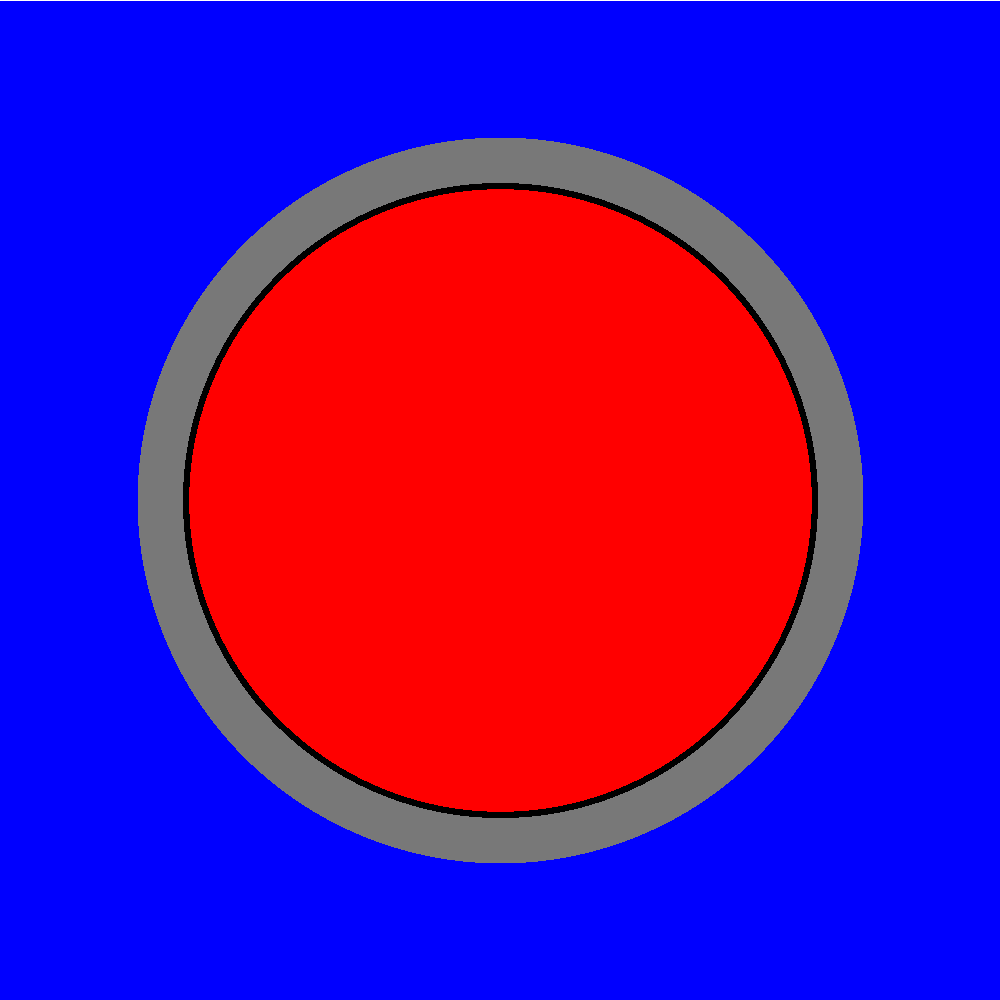
\includegraphics[width=0.9\linewidth]{figures/biases/pin-cell/pin-cell-simple}
  \caption{}
  \label{fig:chap5-pin-a}
\end{subfigure}%
\begin{subfigure}{.32\textwidth}
  \centering
  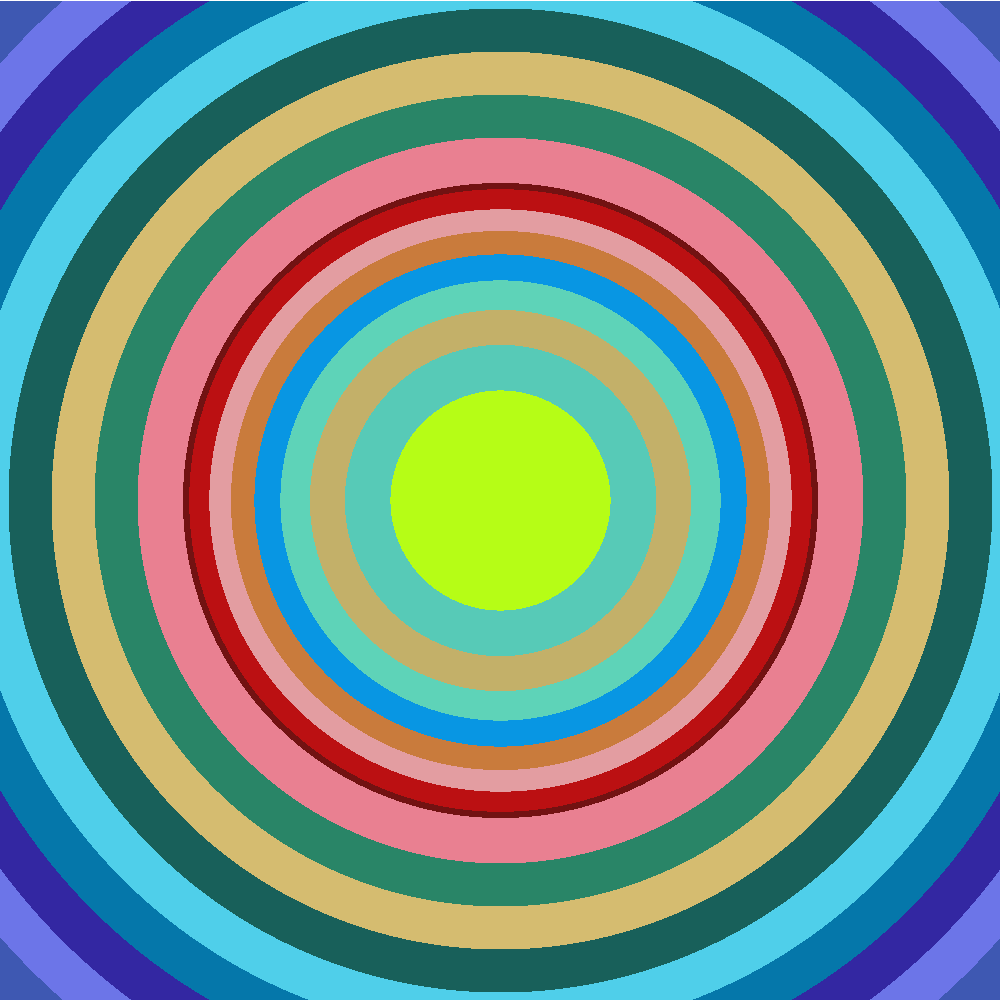
\includegraphics[width=0.9\linewidth]{figures/biases/pin-cell/pin-cell-8x}
  \caption{}
  \label{fig:chap5-pin-b}
\end{subfigure}
\begin{subfigure}{.32\textwidth}
  \centering
  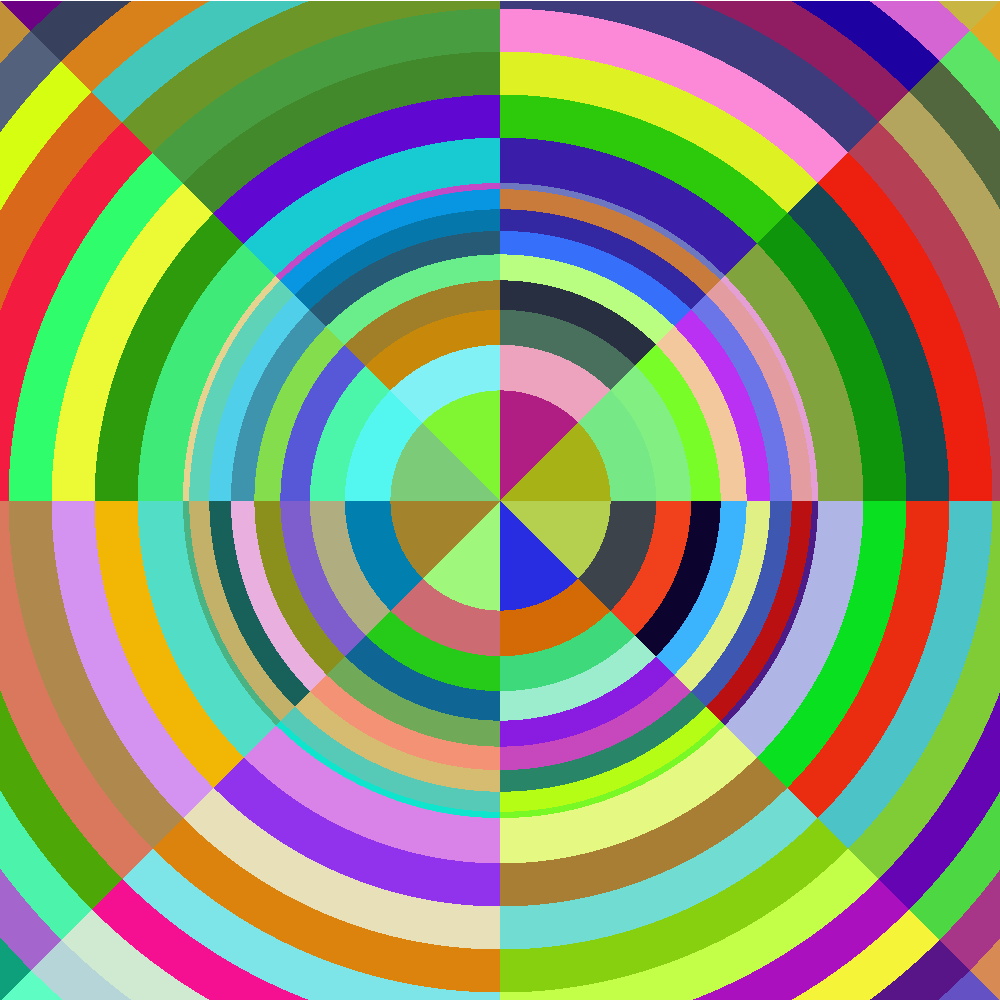
\includegraphics[width=0.9\linewidth]{figures/biases/pin-cell/pin-cell-8x8}
  \caption{}
  \label{fig:chap5-pin-c}
\end{subfigure}
\caption[Pin cell materials and geometry]{A PWR fuel pin cell with fuel, gap, clad and moderator (a). Radial tally zones were defined in each material in OpenMC (b). The tally zones were further subdivided into angular sectors for the \ac{FSR} mesh in OpenMOC (c).}
\label{fig:chap5-pin-cell}
\end{figure}

The reference eigenvalues computed with continuous energy cross sections in OpenMC are shown in Tab.~\ref{table:chap5-pin-reference} for both normal anisotropic and iso-in-lab scattering. The reference calculations were computed for 100 batches of 10$^{7}$ particles per batch. The reference eigenvalues for the two cases vary by 65 \ac{pcm} due to anisotropic thermal scattering in the moderator, roughly the same as that for the 1D slab geometry. The \texttt{openmc.mgxs} module was used to compute 70-group libraries of $\hat{\Sigma}_{t,k,g}$, $\hat{\tilde{\Sigma}}_{t,k,g}$, $\hat{\Sigma}_{s,k,g'\rightarrow g}$, $\hat{\tilde{\Sigma}}_{s,k,g'\rightarrow g}$, $\nu\hat{\Sigma}_{f,g}$, and $\hat{\chi}_{g}$ from OpenMC tallies (see Tab.~\ref{table:chap3-tally-types}). 

\begin{table}[h!]
  \centering
  \caption[Reference $k^{OpenMC}_{eff}$ for a 2D fuel pin]{Reference $k^{OpenMC}_{eff}$ for a 2D fuel pin.}
  \label{table:chap5-pin-reference} 
  \vspace{6pt}
  \begin{tabular}{c c}
  \toprule
  \rowcolor{lightgray}
  {\cellcolor{carolinablue} {\bf Anisotropic}} &
  {\cellcolor{lightgreen} {\bf Isotropic in Lab}} \\
  \midrule
  1.17486 $\pm$ 0.00003 & 1.17421 $\pm$ 0.00002 \\
  \bottomrule
\end{tabular}
\end{table}

%%%%%%%%%%%%%%%%%%%%%%%%%%%%%%%%%%%%%%%%%%%%%%%
\subsubsection{Angular Discretization}
\label{subsubsec:chap5-pin-angle}

The first case study investigated the convergence of the OpenMOC eigenvalue with the angular discretization used in the \ac{MOC} calculation. Tab.~\ref{table:chap5-pin-angle} presents the bias $\Delta\rho$ for a matrix of azimuthal angles and track spacings. Two different 70-group \ac{MGXS} libraries were computed from OpenMC tallies with anisotropic and iso-in-lab scattering. No transport correction was applied to the total cross section $\hat{\Sigma}_{t,k,g}$ or the scattering matrix $\hat{\Sigma}_{s,k,g'\rightarrow g}$. A single radial tally zone was applied to each material for the \ac{MGXS} calculation with OpenMC. The fuel and moderator were each discretized into 5 equal volume radial rings, and each material zone was discretized into 8 angular sectors for the \ac{FSR} mesh in OpenMOC. The results for both normal anisotropic scattering and iso-in-lab scattering exhibit a few hundred \ac{pcm} bias which appears to converge with 128 azimuthal angles and is largely invariant with the track spacing. The \ac{MGXS} tallied with iso-in-lab scattering in OpenMC converge to an eigenvalue that is roughly 95 \ac{pcm} less than that computed for the anisotropic case, with a bias of approximately -170 pcm. Although the bias is of the same order of magnitude as that observed for the 1D slab in Tab.~\ref{table:chap5-slab-angle}, the trend is reversed for anisotropic and isotropic in lab scattering.

\begin{table}[h!]
  \centering
  \caption[Angular discretization error for a 2D fuel pin]{Convergence study of the 70-group eigenvalue bias $\Delta\rho$ with varying azimuthal angle quadratures and track spacings for a 2D fuel pin.}
  \label{table:chap5-pin-angle}
  \vspace{6pt}
  \begin{tabular}{| q | S[table-format=6.1] S[table-format=6.1] S[table-format=6.1] | S[table-format=6.1] S[table-format=6.1] S[table-format=6.1] |}
  \hhline{~|------|}
  \multicolumn{1}{c|}{} &
  \multicolumn{6}{c|}{\cellcolor{lightgray} \bf Track Spacing [cm]} \\
  \multicolumn{1}{c|}{} &
  {\cellcolor{lightgray} \bf 0.1} &
  {\cellcolor{lightgray} \bf 0.01} & 
  \multicolumn{1}{S[table-format=6.1]}{\cellcolor{lightgray} {\bf 0.001}} &
  \multicolumn{1}{S[table-format=6.1]}{\cellcolor{lightgray} {\bf 0.1}} & 
  {\cellcolor{lightgray} \bf 0.01} & 
  \multicolumn{1}{S[table-format=6.1]|}{\cellcolor{lightgray} {\bf 0.001}} \\
  \midrule
  {\bf \# Angles} & \multicolumn{3}{c|}{\cellcolor{carolinablue} \bf Anisotropic} &
  \multicolumn{3}{c|}{\cellcolor{lightgreen} \bf Isotropic in Lab} \\
  \cline{2-7}
4 & 372 & 425 & 427 & 467 & 519 & 521 \\
8 & -377 & -419 & -418 & -282 & -325 & -323 \\
16 & -436 & -408 & -412 & -341 & -314 & -318 \\
32 & -324 & -338 & -331 & -230 & -244 & -236 \\
64 & -256 & -296 & -285 & -162 & -202 & -191 \\
128 & -285 & -276 & -267 & -190 & -182 & -173 \\
256 & -277 & -267 & -265 & -182 & -173 & -171 \\
512 & -273 & -263 & -264 & -179 & -169 & -170 \\
  \bottomrule
\end{tabular}
\end{table}

\newpage

%%%%%%%%%%%%%%%%%%%%%%%%%%%%%%%%%%%%%%%%%%%%%%%
\subsubsection{Energy Condensation and FSR Discretization}
\label{subsubsec:chap5-pin-energy}

The second case study investigated the variation of the OpenMOC eigenvalue with the energy group structure used in the \ac{MOC} calculation. This case study simultaneously varied the \ac{FSR} discretization used in the OpenMOC simulation. The \ac{FSR} mesh in the fuel and moderator consisted of 1 -- 16 equal volume radial rings in each material with 8 angular sectors. The gap and clad were modeled with a single radial zone subdivided into 8 angular sectors. Tab.~\ref{table:chap5-pin-energy} presents the bias $\Delta\rho$ between OpenMC and OpenMOC for a matrix of energy group structures and \ac{FSR} spatial discretizations. In each case, the \ac{MGXS} used in OpenMOC were tallied by material rather than \ac{FSR} in OpenMC (\textit{i.e.}, the spatial tally mesh corresponded to Fig.~\ref{fig:chap5-pin-a}). The OpenMOC calculations used 128 azimuthal angles and 0.01 cm track spacing. Each of the materials in the fuel pin was discretized into 8 angular sectors. The fuel and moderator were each discretized into 1 -- 16 equal volume radial rings. 

\begin{table}[h!]
  \centering
  \caption[Energy and spatial discretization error for a 2D fuel pin]{Convergence study of the eigenvalue bias $\Delta\rho$ with varying energy group structures and \ac{FSR} spatial discretizations for a 2D fuel pin with \textit{\ac{MGXS} tallied by material}.}
  \label{table:chap5-pin-energy} 
  \vspace{6pt}
  \begin{tabular}{| q | S[table-format=6.1] S[table-format=6.1] S[table-format=6.1] S[table-format=6.1] S[table-format=6.1] |}
  \hhline{~|-----|}
  \multicolumn{1}{c|}{\cellcolor{white}} & \multicolumn{5}{c|}{\cellcolor{lightgray} {\bf \ac{FSR} Discretization}} \\
  \multicolumn{1}{c|}{\cellcolor{white}} &
  {\cellcolor{lightgray} {\bf 1$\times$}} &
  {\cellcolor{lightgray} {\bf 2$\times$}} &
  {\cellcolor{lightgray} {\bf 4$\times$}} &
  {\cellcolor{lightgray} {\bf 8$\times$}} &
  {\cellcolor{lightgray} {\bf 16$\times$}} \\
  \midrule
  \multicolumn{1}{|c|}{\cellcolor{lightgray} {\bf \# Groups}} & \multicolumn{5}{c|}{\cellcolor{carolinablue} \bf Anisotropic w/o Transport Correction} \\
  \hhline{~|-----|}
1 & 65 & 66 & 66 & 66 & 66 \\
2 & 21 & -23 & -54 & -65 & -64 \\
4 & -60 & -100 & -129 & -143 & -151 \\
8 & -77 & -137 & -183 & -204 & -215 \\
16 & -74 & -141 & -194 & -219 & -230 \\
25 & -130 & -194 & -245 & -272 & -281 \\
40 & -133 & -201 & -257 & -286 & -296 \\
70 & -134 & -204 & -263 & -294 & {\cellcolor{darktangerine}} -304 \\
  \midrule
  \multicolumn{1}{c|}{\cellcolor{white}} & \multicolumn{5}{c|}{\cellcolor{lightgreen} \bf Anisotropic w/ Transport Correction} \\
  \midrule
1 & 51 & 52 & 52 & 52 & 51 \\
2 & 35 & 6 & -13 & -19 & -11 \\
4 & -60 & -89 & -109 & -125 & -126 \\
8 & -76 & -123 & -158 & -181 & -184 \\
16 & -69 & -124 & -165 & -192 & -196 \\
25 & -126 & -180 & -223 & -249 & -252 \\
40 & -131 & -190 & -239 & -267 & -271 \\
70 & -133 & -194 & -246 & -276 & {\cellcolor{darktangerine}} -280 \\
  \midrule
  \multicolumn{1}{c|}{\cellcolor{white}} & \multicolumn{5}{c|}{\cellcolor{lightsalmonpink} \bf Isotropic in Lab} \\
  \midrule
1 & 79 & 80 & 80 & 80 & 80 \\
2 & 140 & 96 & 65 & 53 & 55 \\
4 & 26 & -14 & -43 & -57 & -65 \\
8 & 25 & -35 & -81 & -102 & -113 \\
16 & 34 & -33 & -86 & -110 & -122 \\
25 & -32 & -95 & -147 & -173 & -182 \\
40 & -39 & -107 & -163 & -192 & -202 \\
70 & -40 & -110 & -169 & -199 & {\cellcolor{darktangerine}} -210 \\
  \bottomrule
\end{tabular}
\end{table}

As was demonstrated for the 1D slab, the results for the fuel pin indicate a strong interaction between the energy and spatial discretization. The eigenvalue bias exhibits a swing of $\sim$350 \ac{pcm} between energy and spatial meshes. The bias exceeds 200 \ac{pcm} for all scattering approximations. The application of the transport correction only reduces the bias by up to 25 \ac{pcm} depending on the energy group structure. The use of the iso-in-lab scattering feature reduces the bias by roughly $\nicefrac{1}{3}$ or 100 pcm. As was observed for the 1D slab, the converged bias is negative for all scattering approximations. 

\clearpage

%%%%%%%%%%%%%%%%%%%%%%%%%%%%%%%%%%%%%%%%%%%%%%%
\subsubsection{Spatial Homogenization and FSR Discretization}
\label{subsubsec:chap5-pin-space}

A final case study was performed to investigate the sensitivity of the OpenMOC eigenvalue to the spatial tally mesh used to compute \ac{MGXS}. This case study was identical to that presented in Sec.~\ref{subsubsec:chap5-pin-energy}, but in this case the \textbf{\ac{MGXS} were computed using a tally mesh in OpenMC identical to the \ac{FSR} mesh used by OpenMOC}. Tab.~\ref{table:chap5-pin-space} presents the bias for a matrix of energy group structures and \ac{MGXS} spatial tally zone meshes. In each case, the \ac{MGXS} were tallied on the \ac{FSR} mesh used in OpenMOC with 1 -- 16 equal volume rings in the fuel and moderator, with a single ring each for the gap and clad (\textit{i.e.}, the spatial tally mesh corresponded to Fig.~\ref{fig:chap5-pin-b}). The OpenMOC calculations used 128 azimuthal angles and 0.01 cm track spacing.

\begin{table}[h!]
  \centering
  \caption[Spatial homogenization error for a 2D fuel pin]{Convergence study of the eigenvalue bias $\Delta\rho$ with varying energy group structures and \ac{FSR} spatial discretizations for a 2D fuel pin with \textit{\ac{MGXS} tallied by \ac{FSR}}.}
  \label{table:chap5-pin-space} 
  \vspace{6pt}
  \begin{tabular}{| q | S[table-format=6.1] S[table-format=6.1] S[table-format=6.1] S[table-format=6.1] S[table-format=6.1] |}
  \hhline{~|-----|}
  \multicolumn{1}{c|}{\cellcolor{white}} & \multicolumn{5}{c|}{\cellcolor{lightgray} {\bf \ac{FSR} Discretization}} \\
  \multicolumn{1}{c|}{\cellcolor{white}} &
  {\cellcolor{lightgray} {\bf 1$\times$}} &
  {\cellcolor{lightgray} {\bf 2$\times$}} &
  {\cellcolor{lightgray} {\bf 4$\times$}} &
  {\cellcolor{lightgray} {\bf 8$\times$}} &
  {\cellcolor{lightgray} {\bf 16$\times$}} \\
  \midrule
  \multicolumn{1}{|c|}{\cellcolor{lightgray} {\bf \# Groups}} & \multicolumn{5}{c|}{\cellcolor{carolinablue} \bf Anisotropic w/o Transport Correction} \\
  \hhline{~|-----|}
1 & 67 & 60 & 63 & 98 & 92 \\
2 & 22 & -27 & -56 & -55 & -51 \\
4 & -58 & -101 & -128 & -128 & -135 \\
8 & -75 & -139 & -182 & -194 & -197 \\
16 & -73 & -142 & -190 & -209 & -207 \\
25 & -128 & -198 & -246 & -271 & -268 \\
40 & -131 & -209 & -261 & -288 & -288 \\
70 & -132 & -214 & -267 & -296 & {\cellcolor{darktangerine}} -297 \\
  \midrule
  \multicolumn{1}{c|}{\cellcolor{white}} & \multicolumn{5}{c|}{\cellcolor{lightgreen} \bf Anisotropic w/ Transport Correction} \\
  \midrule
1 & 53 & 61 & 75 & 66 & 72 \\
2 & 37 & 11 & 1 & -10 & 4 \\
4 & -58 & -83 & -92 & -114 & -109 \\
8 & -74 & -117 & -145 & -175 & -170 \\
16 & -67 & -118 & -154 & -186 & -183 \\
25 & -124 & -181 & -221 & -253 & -245 \\
40 & -130 & -191 & -238 & -272 & -265 \\
70 & -131 & -196 & -245 & -281 & {\cellcolor{darktangerine}} -274 \\
  \midrule
  \multicolumn{1}{c|}{\cellcolor{white}} & \multicolumn{5}{c|}{\cellcolor{lightsalmonpink} \bf Isotropic in Lab} \\
  \midrule
1 & 80 & 92 & 55 & 83 & 66 \\
2 & 141 & 87 & 29 & 50 & 34 \\
4 & 27 & -15 & -43 & -45 & -57 \\
8 & 26 & -34 & -85 & -90 & -102 \\
16 & 35 & -35 & -91 & -101 & -111 \\
25 & -31 & -105 & -158 & -170 & -182 \\
40 & -38 & -114 & -174 & -189 & -202 \\
70 & -39 & -117 & -182 & -196 & {\cellcolor{darktangerine}} -211 \\
  \bottomrule
\end{tabular}
\end{table}

The trends analyzed in Tab.~\ref{table:chap5-pin-energy} emerge in a similar manner with spatially-dependent \ac{MGXS}. In particular, the eigenvalue bias grows in magnitude with more energy groups and \ac{FSR}s but is largely insensitive to the the elimination of the isotropic scattering approximation. As was observed for the 1D slab, the overall systematic error between OpenMC and OpenMOC is not resolved and in fact increases with greater spatial resolution of the \ac{MGXS}. The results in Tab.~\ref{table:chap5-pin-space} indicate that spatial self-shielding effects captured with spatially-varying scalar flux-weighted MGXS for each FSR do not have a substantial impact on the systematic errors in the eigenvalue.

%The eigenvalues for the fine energy and spatial mesh are $\sim$60 \ac{pcm} less than those computed with \ac{MGXS} tallied by material, increasing the magnitude of the bias $\Delta\rho$ by the same amount. The results in Tab.~\ref{table:chap5-pin-space} demonstrate that spatial self-shielding effects captured with spatially-varying scalar flux-weighted \ac{MGXS} for each \ac{FSR} has a larger impact (60 pcm) than was the case for the 1D slab. However, the overall systematic error between OpenMC and OpenMOC is not resolved and in fact increases with greater spatial resolution of the \ac{MGXS}.

\vspace{0.5cm}
\begin{emphbox}
\textbf{A systematic bias of -200 to -300 \ac{pcm} exists between OpenMC and OpenMOC for a 2D fuel pin. The bias varies with the \ac{FSR} discretization and grows with more energy groups. The bias is partially eliminated with iso-in-lab scattering, and is invariant to the spatial mesh used to generate \ac{MGXS}.}
\end{emphbox}

\clearpage

%%%%%%%%%%%%%%%%%%%%%%%%%%%%%%%%%%%%%%%%%%%
%\subsection{2D Fuel Assembly}


%%%%%%%%%%%%%%%%%%%%%%%%%%%%%%%%%%%%%%%%%%%%%%%%%%%%%%%%%%%%%%%%%%%%%%%%%%%%%%%%
\section{Diagnosing the Error}
\label{sec:chap5-diagnosis}

The emergence of a negative systematic bias in the eigenvalue with fine energy and spatial discretization for the heterogeneous 1D slab and 2D fuel pin models led to an analysis of the flux spectra computed by OpenMC and OpenMOC. The 70-group volume-averaged energy-dependent flux in the fuel for both benchmarks is illustrated in Fig.~\ref{fig:chap5-flux}. All of the characteristic trends that one would expect to see in an \ac{LWR} spectra are easily identifiable. In particular, the fission peak at fast energies, the $\nicefrac{1}{E}$ slowing down flux for epithermal energies, and the Maxwellian peak at thermal energies are visible for the slab and fuel pin. The OpenMC flux is barely visible since there is little difference between the two flux spectra when jointly plotted for all groups. The two spectra do appear to differ slightly in the epithermal regime where there is a noticeable degradation in the flux due to resonance capture and scattering. The following sections investigate the deviations in the flux in resonance groups and estimate how they impact the bias in the eigenvalues predicted by OpenMC and OpenMOC.

\begin{figure}
\begin{subfigure}{0.9\textwidth}
  \centering
  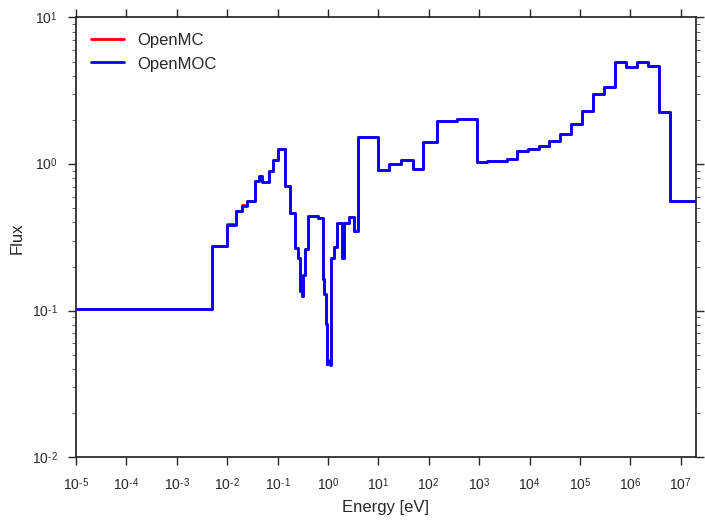
\includegraphics[width=\linewidth]{figures/biases/slab/vol-avg-flux}
  \caption{}
\end{subfigure}
\begin{subfigure}{0.9\textwidth}
  \centering
  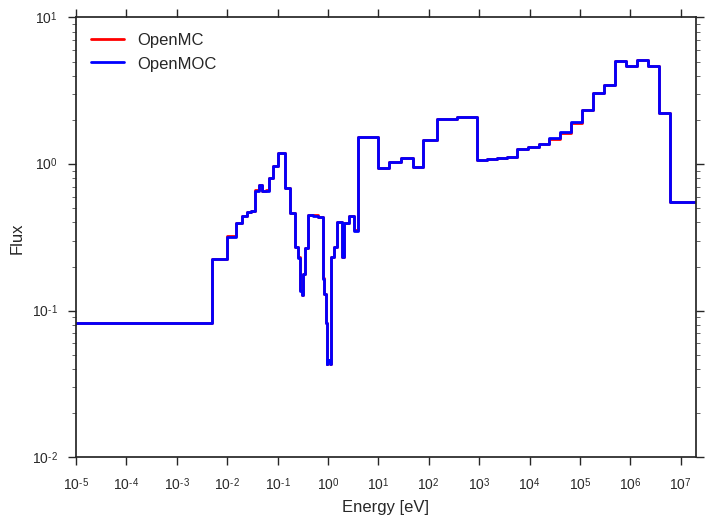
\includegraphics[width=\linewidth]{figures/biases/pin-cell/vol-avg-flux}
  \caption{}
\end{subfigure}
\caption[Flux spectrum in a slab and pin cell]{The flux spectrum in energy in a 1D slab (a) and 2D fuel pin (b).}
\label{fig:chap5-flux}
\end{figure}

%%%%%%%%%%%%%%%%%%%%%%%%%%%%%%%%%%%%%%%%
\subsection{Energy-Dependent Flux Error}
\label{subsec:chap5-diagnosis-energy}

Upon further inspection, it was noted that OpenMOC's flux exhibited large errors with respect to the reference OpenMC flux in those energy groups which isolate large U-238 capture resonances. The error in the 70-group flux is illustrated in Fig.~\ref{fig:chap5-rel-err-energy} for the \ac{FSR}s nearest and furthest from the moderator. These plots were generated for the benchmark models with a 16$\times$ \ac{FSR} discretization with \ac{MGXS} tallied on the \ac{FSR} mesh. The plots correspond to the case studies in Tables~\ref{table:chap5-slab-space} and~\ref{table:chap5-pin-space} with iso-in-lab scattering.

\begin{figure}[h!]
\begin{subfigure}{.9\textwidth}
  \centering
  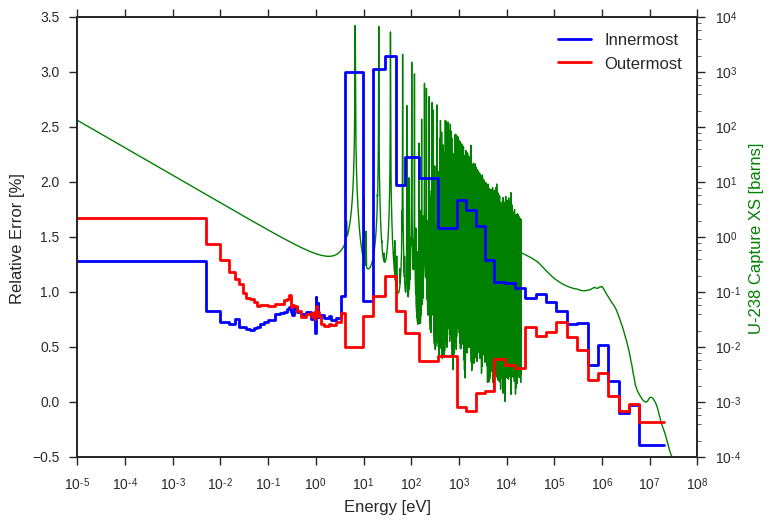
\includegraphics[width=\linewidth]{figures/biases/slab/rel-err-inner-outer}
  \caption{}
\end{subfigure}
\begin{subfigure}{.9\textwidth}
  \centering
  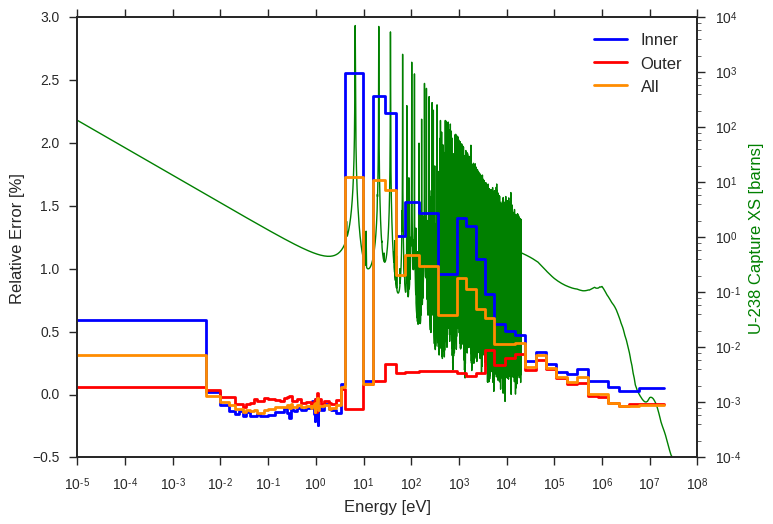
\includegraphics[width=\linewidth]{figures/biases/pin-cell/rel-err-inner-outer}
  \caption{}
\end{subfigure}
\caption[Flux relative error by energy group]{The energy-dependent relative error of the OpenMOC scalar flux with respect to the reference OpenMC flux in a 1D slab (a) and 2D fuel pin (b). The results correspond to the case studies presented in Tables~\ref{table:chap5-slab-space} and~\ref{table:chap5-pin-space}.}
\label{fig:chap5-rel-err-energy}
\end{figure}

As illustrated in the figures, there is a striking error of up to 1.5\% for the fluxes in the slab and up to 2.5\% for the fuel pin in the innermost \ac{FSR} in groups 24, 25 and 27. These energy groups contain the three largest U-238 capture resonances betweeen 4 and 48.052 eV. In addition, the flux errors appear to ``build up'' as the energy decreases through the resonance range, and the magnitude of the capture resonances increase. The one notable exception to this is group 26 (4 -- 9.877 eV) which does not include a U-238 capture resonance. These observations stand in contrast to the flux errors in the outermost \ac{FSR} for which no remarkable trend can be discerned. The positive error in the flux in groups with large capture resonances indicates that capture reaction rates are over-predicted in those groups by OpenMOC, contributing to the negative bias in the eigenvalue. Furthermore, these results indicate a strong relationship between the energy and spatial distribution of the flux errors, as is explored in the following section.

%\begin{emphbox}
%\textbf{The OpenMOC flux exhibits a few percent error in groups with large U-238 capture resonances.}
%\end{emphbox}

%%%%%%%%%%%%%%%%%%%%%%%%%%%%%%%%%%%%%%%%%%%
\subsection{Spatially-Dependent Flux Error}
\label{subsec:chap5-diagnosis-space}

The results presented in Fig.~\ref{fig:chap5-rel-err-energy} indicate significant errors in resonance groups, and in particular, group 27 in the 70-group calculation. Furthermore, the results indicated a large difference in the error profile for those \ac{FSR}s nearest and furthest from the moderator. These trends were studied further to better understand the spatial variation of the flux error across the 16 \ac{FSR}s in the fuel for the slab and pin geometries. In this analysis, the error of the flux was considered in the three different \textit{ranges} of energy group structures itemized below:

\vspace{-0.15cm}
\begin{itemize}[noitemsep]
  \item {\bf Range A} -- group 27 encompassing the U-238 capture resonance at 6.67 eV
  \item {\bf Range B} -- groups 11 -- 27 spanning the resonance range from 4 eV -- 408.5 keV
  \item {\bf Range C} -- groups 1 -- 70 spanning the entire energy regime from 0 -- 20 MeV
\end{itemize}
\vspace{-0.15cm}

Fig.~\ref{fig:chap5-rel-err-space} highlights the spatial dependence of the error across the fuel for each energy range. These plots were generated for the benchmark models with a 16$\times$ \ac{FSR} discretization with \ac{MGXS} tallied on the \ac{FSR} mesh. The plots correspond to the case studies in Tables~\ref{table:chap5-slab-space} and~\ref{table:chap5-pin-space} with iso-in-lab scattering.

The range A error in the slab monotonically decreases from a maximum of nearly 1.5\% to a minimum of $\sim$-0.5\% in those \ac{FSR}s furthest and nearest the moderator, with a similar trend observed for the fuel pin. Furthermore,  the trend accelerates in outermost 3 -- 4 \ac{FSR}s nearest the moderator, where the error drops by nearly half of its value at the center of the slab and pin. The error profiles for energy ranges B and C exhibit the same decreasing trend from the inside to the oustide of the slab and pin, but the error magnitude never exceeds 0.5\% in magnitude. The systematic error trends in energy and space imply that the negative eigenvalue bias is driven by a poor prediction of the reaction rates in resonance groups, as investigated in the following section.

\begin{figure}[H]
\begin{subfigure}{\textwidth}
  \centering
  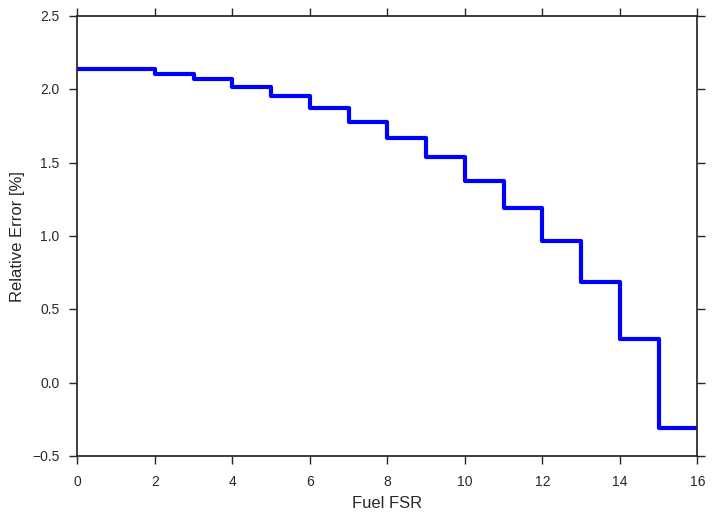
\includegraphics[width=0.8\linewidth]{figures/biases/slab/rel-err-fuel-fsrs}
  \caption{}
\end{subfigure}
\begin{subfigure}{\textwidth}
  \centering
  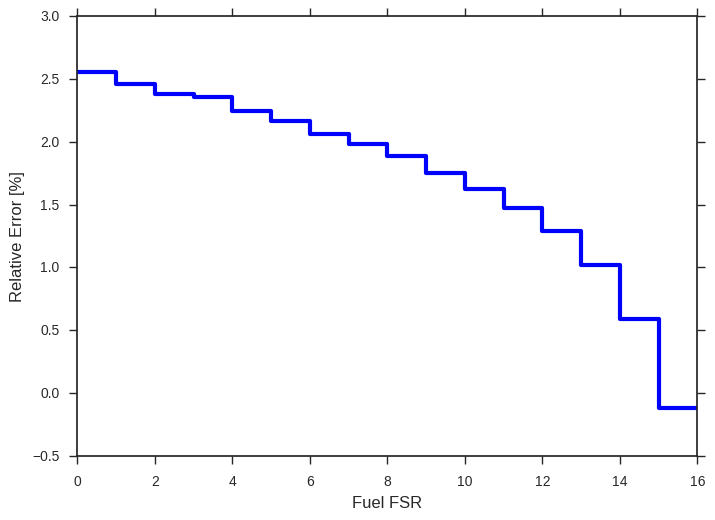
\includegraphics[width=0.8\linewidth]{figures/biases/pin-cell/rel-err-fuel-fsrs}
  \caption{}
\end{subfigure}
\caption[Flux relative error by FSR]{The spatially-varying relative error of the OpenMOC scalar flux with respect to the reference OpenMC flux for a 1D slab (a) and 2D fuel pin (b) in energy Ranges A, B, and C. The results correspond to Tables~\ref{table:chap5-slab-space} and~\ref{table:chap5-pin-space}.}
\label{fig:chap5-rel-err-space}
\end{figure}

Fig.~\ref{fig:chap5-u238-capture-space} illustrates the spatial dependence of the normalized U-238 capture reaction rates in Range A across the fuel for the slab and pin cell. The ``rim effect'' of U-238 capture (and subsequent production of Pu-239) in the outermost ring nearest the moderator is easily seen for both geometries. The capture rates are 5$\times$ greater in the outermost slab/ring than in the innermost slabs/rings. The interior zones experience a highly self-shielded flux since neutrons at energies coinciding with the U-238 capture resonance at 6.67 eV are absorbed in the outermost ring before they can further penetrate the fuel. Although the Range A capture rates in the interior regions are relatively small, the largest errors appear in those zones as shown in Fig.~\ref{fig:chap5-rel-err-space}. Taken together, the reaction rates and flux errors convolve to produce a non-negligible error in the volume-integrated U-238 capture rate across the slab/pin as shown in next section.

\begin{figure}[h!]
  \centering
  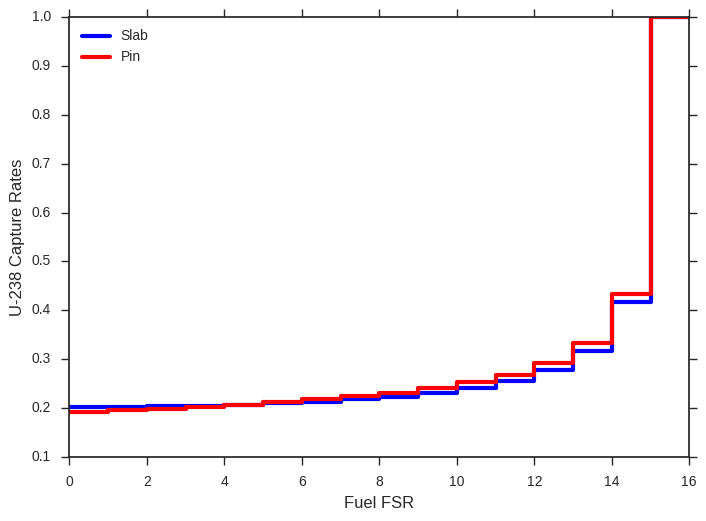
\includegraphics[width=0.8\linewidth]{figures/biases/u238-capt-rates-fuel-fsrs}
  \caption{}
\caption[U-238 capture rates by FSR]{The normalized spatially-varying U-238 capture rates tallied by OpenMC for a 1D slab 2D fuel pin in Range A. The results correspond to Tables~\ref{table:chap5-slab-space} and~\ref{table:chap5-pin-space}.}
\label{fig:chap5-u238-capture-space}
\end{figure}

%\begin{emphbox}
%\textbf{The flux error varies across the fuel in the slab and pin, and is greatest in those \ac{FSR}s nearest the center of the slab and fuel pin.}
%\end{emphbox}

%%%%%%%%%%%%%%%%%%%%%%%%%%%%%%%%%
\subsection{Reaction Rate Errors in the Resonance Regime}
\label{subsec:chap5-diagnosis-rxn-rates}

The errors in the multi-group flux directly correspond to equal errors in the reaction rates since the \ac{MGXS} are computed from the reference reaction rate and flux tallies. The results presented in Figs.~\ref{fig:chap5-rel-err-energy} and \ref{fig:chap5-rel-err-space} revealed significant errors in resonance groups, and in particular, group 27 in the 70-group calculation. In this section, the capture and absorption rate errors are evaluated to quantify how much of the negative eigenvalue bias in the two geometries can be attributed to the mis-predicted reaction rates in the resonance groups. This analysis was performed for different energy group structures to determine if errors in the reaction rates emerge with more energy groups, similar to the eigenvalue bias observed in the case studies in Sec.~\ref{sec:chap5-case-studies}.

The relative error for both U-238 capture and total absorption for all nuclides is quantified in Tab.~\ref{table:chap5-rxn-rate-errors} for energy ranges A, B and C (see Sec.~\ref{subsec:chap5-diagnosis-space}). As in Secs.~\ref{subsec:chap5-diagnosis-energy} and~\ref{subsec:chap5-diagnosis-space}, the analysis considered the slab and fuel pin benchmark models with a 16$\times$ \ac{FSR} discretization with \ac{MGXS} tallied on the \ac{FSR} mesh. The OpenMC iso-in-lab scattering feature was used to generate \ac{MGXS} for OpenMOC.

As illustrated in the table, the U-238 capture and total absorption rate errors each grow with the number of energy groups. This trend is particularly pronounced for U-238 capture in the 6.67 eV resonance group which approaches 0.6\% and 1.35\% for the slab and pin, respectively, when 25 or more groups are used in the multi-group calculation. The 0.08\% and 0.17\% error in the total absorption in range C directly corresponds to an under-prediction in the eigenvalue of 115 and 197 \ac{pcm} for the slab and fuel pin, respectively, which closely matches the observed eigenvalue bias for each model\footnote{This analysis neglects the contribution of scattering multiplicity (\textit{e.g.,} (n,xn)) to the eigenvalue.}. Approximately 5 -- 6\% and 16 -- 18\% of the total absorption occurs in energy ranges A and B, with U-238 capture accounting for 80\% and 70\% of the total absorption in each energy range, respectively. Hence, the error in U-238 resonance capture alone under-predicts the eigenvalue by 105 and 145 \ac{pcm} for the slab and pin, with approximately half of the error deriving from group 27 of 70 due to the resonance at 6.67 eV. 

%U-238 capture
%slab 27: 50 pcm
%slab all: 105 pcm
%pin 27: 100 pcm
%pin all: 185 pcm

%The total energy-integrated fission rate error is $\sim$1\% and $\sim$0.25\% for the slab and pin (and over 2\% in group 27) which would correspond to an over-prediction in the eigenvalue of

%Taken together, the errors in the absorption and fission rates would result in an eigenvalue bias that compares closely with the observed $\Delta\rho \approx$ 300 -- 350 \ac{pcm} \footnote{This analysis neglects the contribution of scattering multiplicity (\textit{e.g.,} (n,2n)) to the eigenvalue.}.

%Fig.~\ref{fig:chap5-pin-fuel-fsrs} highlights the spatial dependence of the error in group 27 across the fuel which isolates the largest U-238 capture resonance at 6.67 eV. The error decreases from a maximum of $\sim$2.8\% to a minimum of $\sim$0.6\% in those \ac{FSR}s furthest and nearest the moderator, respectively. It is unclear why the spatial dependence of the error does not monotonically decrease across the fuel pin as it does for the slab (see Fig.~\ref{fig:chap5-slab-fuel-fsrs}), but the overall trend is the same.

{\setlength{\extrarowheight}{-5pt}
\begin{table}[H]
  \centering
  \caption[Reaction rate relative errors]{The volume-integrated U-238 capture and total absorption rate percent relative errors. The errors correspond to the results in Tables~\ref{table:chap5-slab-space} and \ref{table:chap5-pin-space}.}
  \small
  \label{table:chap5-rxn-rate-errors} 
  \vspace{6pt}
  \begin{tabular}{| q | S[table-format=5.1] S[table-format=5.1] S[table-format=5.1] | S[table-format=5.1] S[table-format=5.1] S[table-format=5.1] |}
  \hhline{~|------|}
  \multicolumn{1}{c|}{\cellcolor{white}} &
  \multicolumn{3}{c|}{\cellcolor{lightgray} {\bf U-238 Capture}} &
  \multicolumn{3}{c|}{\cellcolor{lightgray} {\bf Total Absorption}} \\
  \multicolumn{1}{c|}{\cellcolor{white}} &
  {\bf \cellcolor{lightgray} Range A} &
  {\bf \cellcolor{lightgray} Range B} &
  {\bf \cellcolor{lightgray} Range C} &
  {\bf \cellcolor{lightgray} Range A} &
  {\bf \cellcolor{lightgray} Range B} &
  {\bf \cellcolor{lightgray} Range C} \\
  \midrule
  \multicolumn{1}{|c|}{\cellcolor{lightgray} {\bf \# Groups}} &
  \multicolumn{6}{c|}{\cellcolor{carolinablue} {\bf 1D Slab}} \\
  \hhline{~|------|}
1 & -0.02 & -0.02 & -0.02 & -0.11 & -0.11 & -0.11 \\
2 & 0.05 & 0.05 & 0.03 & 0.05 & 0.05 & -0.07 \\
4 & 0.11 & -0.08 & 0.06 & 0.12 & -0.08 & -0.05 \\
8 & 0.19 & -0.03 & 0.11 & 0.22 & -0.03 & 0.00 \\
16 & 0.21 & -0.02 & 0.12 & 0.23 & -0.02 & 0.02 \\
25 & 0.58 & 0.36 & 0.26 & 0.61 & 0.37 & 0.06 \\
40 & 0.58 & 0.43 & 0.30 & 0.61 & 0.44 & 0.07 \\
70 & {\cellcolor{darktangerine}} 0.59 & 0.46 & 0.30 & 0.61 & 0.47 & 0.08 \\
  \midrule
  \multicolumn{1}{c|}{\cellcolor{white}} & 
  \multicolumn{6}{c|}{\cellcolor{lightgreen} {\bf 2D Fuel Pin}} \\
  \midrule
1 & -0.02 & -0.02 & -0.02 & -0.07 & -0.07 & -0.07 \\
2 & 0.11 & 0.11 & 0.07 & 0.11 & 0.11 & -0.03 \\
4 & 0.55 & 0.07 & 0.32 & 0.54 & 0.07 & 0.04 \\
8 & 0.71 & 0.11 & 0.40 & 0.72 & 0.11 & 0.08 \\
16 & 0.72 & 0.12 & 0.41 & 0.73 & 0.12 & 0.09 \\
25 & 1.32 & 0.85 & 0.61 & 1.34 & 0.85 & 0.15 \\
40 & 1.33 & 0.93 & 0.64 & 1.34 & 0.92 & 0.16 \\
70 & {\cellcolor{darktangerine}} 1.33 & 0.99 & 0.65 & 1.35 & 0.97 & 0.17 \\
  \bottomrule
\end{tabular}
\end{table}}

These results indicate that spatial self-shielding effects in resonance groups is not adequately captured by the \ac{MGXS} and/or the multi-group calculation. Furthermore, this analysis illustrates the counter-intuitive result that the bias between continuous energy Monte Carlo and multi-group deterministic transport may in fact increase in magnitude with more energy groups. Although it is challenging to isolate the factors which convolve to bias the eigenvalue, the data presented here indicates that an over-prediction of U-238 capture in the resonance groups largely drives the error. These results will be discussed in greater depth in the context of angular-dependent \ac{MGXS} in Chapter~\ref{chap:sph}.

\begin{emphbox}
\textbf{The negative eigenvalue bias is caused by an over-prediction of absorption, dominated by U-238 capture in the 6.67 eV resonance. The reaction rate error increases with more energy groups as observed for the eigenvalue bias.}
\end{emphbox}

\clearpage

\vfill
\begin{highlightsbox}[frametitle=Highlights]
\begin{itemize}
  \item OpenMOC calculations were performed using \ac{MGXS} generated by OpenMC to compare eigenvalues for simple benchmarks.
  \item The eigenvalues closely agreed for homogeneous infinite media. The eigenvalues exhibited a bias of -200 to -300 \ac{pcm} for heterogenous geometries, including a 1D slab and 2D fuel pin.
  \item A series of case studies demonstrated the dependence of the bias with:
  \begin{itemize}
%    \item \textit{\ac{FSR} discretization} -- The bias was jointly-dependent with energy group structure.
    \item \textit{Energy condensation} -- The bias increased with more energy groups due to systematic errors in groups with large U-238 capture resonances.
    \item \textit{Spatial homogenization} -- The spatial tally mesh used to generate \ac{MGXS} in the fuel and moderator had no effect on the bias.
    \item \textit{Angular treatment} -- \ac{MGXS} generated with iso-in-lab scattering in OpenMC reduced the bias by $<$100 \ac{pcm} or $\sim\frac{1}{3}$.
  \end{itemize} 
  \item The eigenvalue bias is largely attributable to an over-prediction of U-238 capture rates in resonance groups.
  \item The flux errors indicate that spatial self-shielding is not adequately modeled in spatially heterogeneous multi-group calculations even when the ``true'' scalar flux is used to compute \ac{MGXS}.
\end{itemize}
\end{highlightsbox}
\vfill
\chapter{Angular-Dependent MGXS}
\label{chap:sph}

The results in Chapter~\ref{chap:biases} demonstrated that using the ``true'' flux spectrum from Monte Carlo to perform energy condensation and spatial homogenization will not necessarily result in accurate deterministic multi-group calculations. Large systematic biases in the eigenvalue were observed even for simple heterogeneous benchmark models, and these biases were highly dependent on the energy group structure and spatial discretization used in the multi-group deterministic calculation. In Section~\ref{sec:chap4-diagnosis} it was shown that the bias largely derives from errors in the multi-group reaction rates in the large thermal U-238 capture resonances, and that the errors systematically vary in space within the fuel. These results indicate that one or more of the approximations made in multi-group transport theory are invalidated in heterogeneous geometries and prevents spatial self-shielding at the fuel/moderator interface in \ac{PWR} geometries to be treated appropriately.

Although Chapter~\ref{chap:biases} quantified energy and spatial approximations in multi-group theory, it did not consider the constant-in-angle approximation (see Section~\ref{subsubsec:chap2-const-in-angle}). This chapter reviews some recent work by by Gibson~\cite{gibson2016thesis} to quantify the approximation error resolved with angular dependent \ac{MGXS}, which closely mirrors the trends observed in Chapter~\ref{chap:biases}. The historical \ac{SPH} factor concept is introduced in the context of angular-dependent \ac{MGXS}, and \ac{SPH} factors are applied to simple heterogeneous benchmarks and the results analyzed. Finally, this chapter concludes with a summary of the shortcomings of the \ac{SPH} approach and the need for new methods to account for the angular dependence in \ac{MGXS}.

%Chapter~\ref{chap:mgxs} detailed the approximations made in the multi-group form of the transport equation. 


%%%%%%%%%%%%%%%%%%%%%%%%%%%%%%%%%%%%%%%%%%%%%%%%%%%%%%%%%%%%%%%%%%%%%%%%%%%%%%%
\section{Background}
\label{sec:chap5-background}

The results in Chapter~\ref{chap:biases} demonstrated systematic biases between continuous energy Monte Carlo and deterministic multi-group simulations of simple heterogeneous benchmark models. In Section~\ref{sec:chap4-diagnosis} it was shown that these biases largely derive from errors in the multi-group fluxes/reaction rates in the large thermal U-238 capture resonances. 

-sentence wrapping this paragraph up - talk about spatial self-shielding and segue

These results closely mirror observations by Gibson~\cite{gibson2016thesis} which quantified the errors fundamental to the total 

 illustrated 

\begin{itemize}[noitemsep]
  \item return to angular vs. flux weighting (Section~\ref{subsubsec:chap2-const-in-angle})
  \item Gibson's ``batman'' plot and results
  \item Nelson's 1D slab plot(s)?
\end{itemize}

\cite{gibson2016thesis}


\begin{figure}[H]
\begin{subfigure}{.5\textwidth}
  \centering
  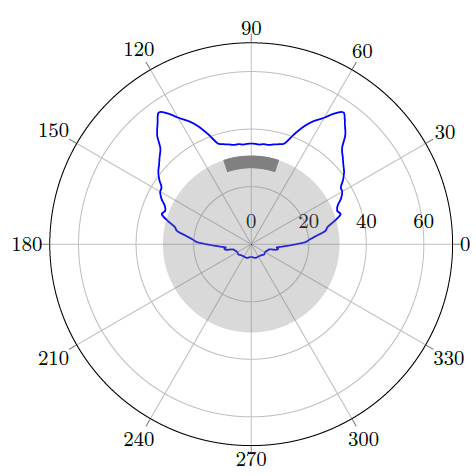
\includegraphics[width=\linewidth]{figures/sph/batman-1}
  \caption{}
\end{subfigure}
\begin{subfigure}{.5\textwidth}
  \centering
  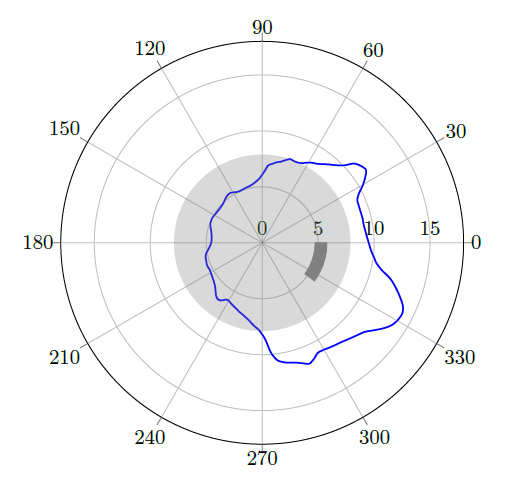
\includegraphics[width=\linewidth]{figures/sph/batman-2}
  \caption{}
\end{subfigure}
\caption[Batman plots]{Cool plots of angular-dependent \ac{MGXS}.}
\label{fig:chap4-rel-err-energy}
\end{figure}

\cite{hebert1993consistent}


%%%%%%%%%%%%%%%%%%%%%%%%%%%%%%%%%%%%%%%%%%%%%%%%%%%%%%%%%%%%%%%%%%%%%%%%%%%%%%%
\section{SuPerHomogenisation Factors}
\label{sec:chap5-sph}

\begin{itemize}
  \item diagnose issue w/ Figures 7.2 and 7.3 from Nate's thesis
  \item introduce basic eqns, reference Hebert
  \item overview algorithm
\end{itemize}


%%%%%%%%%%%%%%%%%%%%%%%%%%%%%%%%%%%%%%%%%%%%%%%%%%%%%%%%%%%%%%%%%%%%%%%%%%%%%%%
\section{SPH Implementation in OpenMOC}
\label{sec:chap5-sph-openmoc}


\begin{landscape}
\begin{algorithm}[!ht]
\caption{Transport Sweep Algorithm}
\label{alg:transport-sweep}
\begin{algorithmic}
    \State $\Phi_{i,g} \gets 0 \;\;\;\; \forall \; i,g \in \{I,G\}$ \Comment{Initialize FSR scalar fluxes to zero}
    \While{$\Phi_{i,g} \; \forall\; i$ not converged}
        \ForAll{$m \in M$}\Comment{Loop over azimuthal angles}
            \ForAll{$k \in K(m)$}\Comment{Loop over tracks}
                \ForAll{$s \in S(k)$}\Comment{Loop over segments}
                    \ForAll{$g \in G$}\Comment{Loop over energy groups}
                        \ForAll{$p \in P$}\Comment{Loop over polar angles}
                            \State $i \gets I(s)$\Comment{Get FSR for this segment}
                            \State $\Delta\Psi_{k,i,g,p} \gets \left(\Psi_{k,g,p} - \frac{Q_{i,g}}{\Sigma^T_{i,g}}\right)(1 - e^{-\tau_{k,i,g,p}})$ \Comment{Compute angular flux change along segment}
                            \State $\Phi_{i,g} \gets \Phi_{i,g} + \frac{4\pi}{A_i} \omega_{m}\omega_{p}\omega_{k}\sin\theta_{p}\Delta\Psi_{k,i,g,p}$ 
                            \Comment{Increment FSR scalar flux}
                            \State $\Psi_{k,g,p} \gets \Psi_{k,g,p} - \Delta\Psi_{k,g,p}$ \Comment{Update track outgoing flux}
                        \EndFor
                    \EndFor
                \EndFor
            \EndFor
            \If{B.C. are reflective}\Comment{Set incoming flux for outgoing track}
                \State $\Psi_{k',g,p}(0) \gets \Psi_{k,g,p}$  
                \Comment{Reflective B.C.'s}
            \Else
                \State $\Psi_{k',g,p}(0) \gets 0$ \Comment{Vacuum B.C.'s}
                \State $L \gets L + \Psi_{k,g,p}$
            \EndIf
        \EndFor
        \State Update $k_{eff}$ and FSR sources $Q_{i,g} \;\forall\; i$ \Comment{\autoref{alg:source-update}}
    \EndWhile
\end{algorithmic}
\end{algorithm}
\end{landscape}



%%%%%%%%%%%%%%%%%%%%%%
\section{Case Studies}
\label{sec:chap5-sph-results}

%%%%%%%%%%%%%%%%%%%%
\subsection{1D Slab}
\label{subsubsec:chap5-sph-slab}

\begin{itemize}[noitemsep]
  \item plot of fluxes w/ and w/o SPH
  \item plot of Nelson's flux/angular-dependent MGXS???
  \item table of SPH factors in group 27 by group structure
  \item re-generate table of data for slab with bigger moderator
  \item eigenvalues if SPH factors for only group 27 are applied
\end{itemize}

\begin{table}[h!]
  \centering
  \caption{Spatial homogenization error with SPH for a 1D slab.}
  \label{table:chap5-sph-slab-energy} 
  \vspace{14pt}
  \begin{tabular}{c S[table-format=6.1] S[table-format=6.1] S[table-format=6.1] S[table-format=6.1] S[table-format=6.1]}
  \toprule
  & \multicolumn{5}{c}{\boldmath $\Delta\rho$ {\bf [pcm]}} \\
  \midrule  
  \multicolumn{1}{c}{\textbf{\# Groups}} &
  \multicolumn{1}{c}{\bf 1$\times$} &
  \multicolumn{1}{c}{\bf 2$\times$} &
  \multicolumn{1}{c}{\bf 4$\times$} &
  \multicolumn{1}{c}{\bf 8$\times$} &
  \multicolumn{1}{c}{\bf 16$\times$} \\
  \midrule
  & \multicolumn{5}{c}{\bf Without SPH} \\
  \cline{2-6}
1 & 585 & 608 & 589 & 589 & 590 \\
2 & 1467 & 852 & 449 & 272 & 238 \\
4 & 1352 & 786 & 421 & 261 & 218 \\
8 & 1686 & 894 & 334 & 92 & 20 \\
16 & 1777 & 932 & 318 & 55 & -26 \\
25 & 1685 & 863 & 251 & 3 & -77 \\
40 & 1721 & 873 & 236 & -25 & -110 \\
70 & 1735 & 881 & 235 & -32 & -122 \\
%1 & 27 & 16 & 12 & 5 & -3 \\
%2 & 58 & 33 & 31 & 21 & 18 \\
%4 & -144 & -156 & -161 & -158 & -156 \\
%8 & -181 & -194 & -200 & -202 & -198 \\
%16 & -180 & -195 & -203 & -204 & -200 \\
%25 & -326 & -331 & -338 & -336 & -336 \\
%40 & -348 & -351 & -359 & -357 & -358 \\
%70 & -355 & -359 & -366 & -364 & -366 \\
  \cline{2-6}
  & \multicolumn{5}{c}{\bf With SPH} \\
  \cline{2-6}
1 & 62 & 107 & 94 & 94 & 95 \\
2 & 61 & 186 & 128 & 67 & 65 \\
4 & 48 & 178 & 136 & 83 & 76 \\
8 & 59 & 226 & 130 & 46 & 27 \\
16 & 62 & 238 & 128 & 38 & 14 \\
25 & 64 & 241 & 123 & 44 & 21 \\
40 & 67 & 248 & 126 & 42 & 17 \\
70 & 67 & 253 & 129 & 44 & 15 \\
%1 & 25 & 12 & 5 & -3 & -12 \\
%2 & 30 & 12 & 13 & 2 & -2 \\
%4 & 17 & 4 & -2 & 2 & 2 \\
%8 & 17 & 6 & -0 & 0 & 1 \\
%16 & 17 & 7 & -1 & -0 & 1 \\
%25 & 9 & 8 & 4 & 4 & 1 \\
%40 & 10 & 9 & 3 & 3 & -1 \\
%70 & 10 & 8 & 4 & 4 & -1 \\
  \bottomrule
\end{tabular}
\end{table}

\begin{table}[h!]
  \centering
  \caption[SPH factors for a 1D slab]{SPH factors in the energy group encompassing the U-238 capture resonance at 6.67 eV for different energy group structures. The SPH factors were computed for a 1D slab and 2D fuel pin without spatial discretization and with ``iso-in-lab'' scattering.}
  \small
  \label{table:chap5-sph-group-27}
  \vspace{6pt}
  \begin{tabular}{c c S[table-format=2.1] S[table-format=2.1]}
  \toprule
  \multicolumn{1}{c}{\textbf{\# Groups}} &
  \multicolumn{1}{c}{\textbf{Group 27}} &
  \multicolumn{2}{c}{\textbf{SPH Factor $\mu$}} \\
  \midrule
  & & \multicolumn{1}{c}{\bf 1D Slab} &
  \multicolumn{1}{c}{\bf 2D Fuel Pin} \\
  \midrule
1 & & & \\
2 & & & \\
4 & & & \\
8 & & & \\
16 & & & \\
25 & & & \\
40 & & & \\
70 & & & \\
  \bottomrule
\end{tabular}
\end{table}


%%%%%%%%%%%%%%%%%%%%%%%%%%%%%
\subsection{2D Fuel Pin Cell}
\label{subsubsec:chap5-sph-pin}

\begin{itemize}[noitemsep]
  \item table of eigenvalues by energy group w/ and w/o SPH
  \item plot of flux errors with U-238 capture XS w/ and w/o SPH
  \item table of SPH factors in group 27 by energy group structure
\end{itemize}

\begin{table}[h!]
  \centering
  \caption{Spatial homogenization error with SPH for a 2D fuel pin.}
  \label{table:chap5-sph-pin-energy} 
  \vspace{14pt}
  \begin{tabular}{c S[table-format=6.1] S[table-format=6.1] S[table-format=6.1] S[table-format=6.1] S[table-format=6.1]}
  \toprule
  & \multicolumn{5}{c}{\boldmath $\Delta\rho$ {\bf [pcm]}} \\
  \midrule  
  \multicolumn{1}{c}{\textbf{\# Groups}} &
  \multicolumn{1}{c}{\bf 1$\times$} &
  \multicolumn{1}{c}{\bf 2$\times$} &
  \multicolumn{1}{c}{\bf 4$\times$} &
  \multicolumn{1}{c}{\bf 8$\times$} &
  \multicolumn{1}{c}{\bf 16$\times$} \\
  \midrule
  & \multicolumn{5}{c}{\bf Without SPH} \\
  \cline{2-6}
1 & 91 & 92 & 92 & 92 & 92 \\
2 & 153 & 109 & 78 & 67 & 68 \\
4 & 31 & -9 & -38 & -51 & -59 \\
8 & 31 & -29 & -75 & -95 & -106 \\
16 & 41 & -26 & -79 & -103 & -114 \\
25 & -27 & -91 & -142 & -169 & -177 \\
40 & -34 & -103 & -159 & -187 & -196 \\
70 & -35 & -106 & -165 & -195 & -204 \\
  \cline{2-6}
  & \multicolumn{5}{c}{\bf With SPH} \\
  \cline{2-6}
1 & 6 & 6 & 6 & 6 & 6 \\
2 & 32 & 32 & 32 & 32 & 32 \\
4 & 7 & 7 & 7 & 7 & 7 \\
8 & 5 & 5 & 5 & 5 & 5 \\
16 & 6 & 6 & 6 & 6 & 6 \\
25 & 8 & 8 & 8 & 8 & 8 \\
40 & 7 & 7 & 7 & 7 & 7 \\
70 & 8 & 8 & 8 & 8 & 8 \\
  \bottomrule
\end{tabular}
\end{table}


%%%%%%%%%%%%%%%%%%%%%%%%%%%%%%%%%%%%%%%%%%%
%\subsection{2D Heterogeneous Fuel Assembly}
%\label{subsec:chap5-sph-hetero-lat}

%\begin{itemize}[noitemsep]
%  \item table of eigenvalues by energy group w/ and w/o SPH
%  \begin{itemize}[noitemsep]
%    \item cell-avg SPH, region-avg SPH, region-clustered (LNS?) SPH
%  \end{itemize}
%  \item bar chart / rug plot of SPH factors in resonance group(s)
%\end{itemize}

%%%%%%%%%%%%%%%%%%%%%%%
\section{Shortcomings of SPH}
\label{subsec:chap5-sph-shortcomings}



\part{Statistical Clustering}
\chapter{Benchmark Models and Reference Results}
\label{chap:benchmarks}

%%%%%%%%%%%%%%%%%%%%%%%%%%%%%%%%%%%%%%%%%%%%%%%%%%%%%%%%%%%%%%%%%%%%%%%%%%%%%%%
\section{Motivation}
\label{sec:chap7-motivate}

This thesis is motivated by the desire to obtain Monte Carlo-quality solutions with computationally efficient deterministic neutron transport methods. In particular, this work evaluates the use of \ac{MC} for reactor agnostic \ac{MGXS} generation for high-fidelity neutron transport simulations. The analysis in Part III was dedicated to the evaluation of approximation errors in \ac{MGXS} and multi-group transport methods which appear in the modeling of even simple heterogeneous benchmarks such as a 2D fuel pin cell. The chapters in Part IV develop a new approach based upon statistical clustering to capture spatial self-shielding effects which occur only in large, complex heterogeneous geometries. This chapter presents several heterogeneous \ac{PWR} benchmark models which are used to evaluate the efficacy of the new methodology for \ac{MGXS} generation throughout the subsequent chapters in Part IV.

Each of the heterogeneous benchmarks presented here is derived from the Benchmark for Evaluation And Validation of Reactor Simulations (BEAVRS) \ac{PWR} model~\cite{horelik2013beavrs}. A series of six benchmarks were designed to introduce increasingly complex heterogeneous features -- and corresponding spatial self-shielding effects -- to the models in order to understand their implications for accurate pin-wise \ac{MGXS} generation. The impact of fuel enrichment, \acp{CRGT}, \acp{BP}, inter-assembly currents, water reflectors, steel baffles and the core barrel and vessel is considered. This chapter details the geometric and material specifications for the individual fuel assemblies, multiple assembly colorsets, and full \ac{BEAVRS} core modeled with different \ac{MGXS} generation schemes throughout Part IV.

In addition, this chapter presents the reference results for each of the six geometries used to evaluate the accuracy of \ac{MGXS} generation with statistical clustering. Since this thesis aims to enable \ac{MC} accuracy in deterministic transport simulations, OpenMC was used to generate the reference results for each of the six benchmarks. This chapter quantifies the source convergence rate for each of the benchmark models using Shannon entropy. In addition, a series of OpenMC simulations were used to calculate reference eigenvalues, pin-wise fission rates, and pin-wise U-238 capture rates for each benchmark.

The eigenvalue is a key integral quantity used to assess the reactivity of a reactor. The fission rates are directly related to the relative power density of each fuel pin which is important for fuel depletion as well as thermal hydraulic feedback. The U-238 capture rates result in the production of Pu-239 which contributes up to 40\% of the power produced from fission in \ac{PWR}s at the end-of-life (EOL). Hence, the spatial distributions of the fission rates and U-238 capture rates must be correctly modeled for accurate high-fidelity depletion calculations. The reference results for each of these three metrics were computed with highly converged OpenMC simulations. It is important to recall from Sec.~\ref{sec:chap1-objectives} that this thesis aimed to generate \ac{MGXS} with \ac{MC} in significantly less time\footnote{In this case, ``time'' is synonymous with the number of particle histories simulated with \ac{MC}.} than would be required to generate reference solutions with \ac{MC}. The methodology developed in Part IV aims to make this possible with statistical clustering of ``noisy'' \ac{MC} tallies for \ac{MGXS} generation.

This chapter outlines the geometric and isotopic specifications for each of the six benchmark models in Sec.~\ref{sec:chap7-benchmarks}. The reference results computed with OpenMC for each of the benchmark models are presented in Sec.~\ref{sec:chap7-ref-results}.


%%%%%%%%%%%%%%%%%%%%%%%%%%%%%%%%%%%%%%%%%%%%%%%%%%%%%%%%%%%%%%%%%%%%%%%%%%%%%%%
\section{Benchmark Configurations}
\label{sec:chap7-benchmarks}

The heterogeneous benchmarks modeled throughout Part IV were based on the \ac{BEAVRS} \ac{PWR} model~\cite{horelik2013beavrs}. The \ac{BEAVRS} model is a highly-detailed \ac{PWR} specification which was created to validate high-fidelity core analysis methods. Five of the six benchmark models are based upon sub-components (\textit{e.g.}, fuel assemblies) of the full core \ac{BEAVRS} model, while the sixth benchmark is of the full \ac{BEAVRS} core model. Although \ac{BEAVRS} is an axially heterogeneous 3D core model, each of the benchmarks were fabricated in 2D due to the geometric constraints in OpenMOC. In particular, the 2D radial heterogeneity in each benchmark is taken from the axial mid-plane of the \ac{BEAVRS} model. The geometries used two planar surfaces perpendicular to the $z$-axis with reflective \acp{BC} to model the benchmarks as infinitely long in the axial direction (\textit{e.g.}, each benchmark is infinitely homogeneous along the $z$-axis).

%first paragraph: refer to the \ac{BEAVRS} model~\cite{horelik2013beavrs}
%-\ac{BEAVRS} consists of fuel assemblies with four different enrichments and various
%  -sliced to encompass the spacer grid
%    -designed model to stress the geometric modeling capabilities of OpenMC/MOC/CG
%    -grid spacers main axial heterogeneities that induce spatial self-shielding in \ac{LWR}s
%    -stress geometric modeling capabilities since framework developed to eventually support 3D \ac{MOC}
%-HZP

The materials and isotopic compositions in each of the benchmarks are detailed in Sec.~\ref{subsec:chap7-materials}, while the geometric specifications for each pin cell type -- fuel pin, instrument tube, \ac{CRGT} and \ac{BP} -- are tabulated in Sec.~\ref{subsec:chap7-pin-cells}. The first three benchmarks were based upon individual \ac{BEAVRS} fuel assemblies with different fuel enrichments and \ac{CRGT} and \ac{BP} locations as discussed in Sec.~\ref{subsec:chap7-fuel-assms}. The geometric configuration of 2$\times$2 fuel assembly colorsets with and without a water reflector are highlighted in Sec.~\ref{subsec:chap7-2x2-colorsets}. Finally, the key parameters for the full \ac{BEAVRS} core model are presented in Sec.~\ref{subsec:chap7-full-core}.


%%%%%%%%%%%%%%%%%%%%%%%%%%%%
\subsection{Materials}
\label{subsec:chap7-materials}

The models described in this section were comprised of materials from the \ac{BEAVRS} model. The six benchmarks include 1.6\%, 2.4\% and 3.1\% enriched UO$_2$ fuel, borated water\footnote{The water consisted of 975 parts per million (ppm) boron, the critical concentration for the all rods out configuration~\cite{horelik2013beavrs}}, zircaloy, helium, air, borosilicate glass and stainless steel. The densities and isotopic compositions for each material are detailed in the \ac{BEAVRS} specifications~\cite{horelik2013beavrs} and are reproduced in App.~\ref{sec:beavrs-materials}. Each of the materials was modeled with cross sections at 600K for hot zero power (HZP) conditions.

%\vspace{-1em}

%\begin{itemize}[noitemsep,topsep=0pt]
%  \setlength\itemsep{-0.6em}
%  \item 1.6\% and 3.1\% enriched UO$_2$ fuel
%  \item Borated water\footnote{The water consisted of 975 parts per million (ppm) boron, the critical concentration for the all rods out configuration~\cite{horelik2013beavrs}.}
%  \item Zircaloy 4
%  \item Helium
%  \item Air
%  \item Borosilicate glass
%  \item Stainless steel (SS304)
%\end{itemize}

%%%%%%%%%%%%%%%%%%%%%%%%%%%%
\subsection{Pin Cells}
\label{subsec:chap7-pin-cells}

The six benchmarks were composed of four different types of pin cells -- fuel pins, instrument tubes, control rod guide tubes and burnable poisons. Each of the four pin cell types is displayed in Fig.~\ref{fig:chap7-pin-cells}. The different material types are indicated with different colors. The fuel pin in Fig.~\ref{fig:chap7-pin-1.6} contains UO$_2$ fuel, a helium gap and zircaloy cladding. The \ac{CRGT} in Fig.~\ref{fig:chap7-pin-crgt} is modeled in the control rod out configuration from above the dashpot and includes borated water surrounded by zircaloy cladding. The instrument tube in Fig.~\ref{fig:chap7-instr-tube} is filled with air surrounded by two tubes of zircaloy cladding separated by borated water. The \ac{BP} in Fig.~\ref{fig:chap7-bp} is the geometry from above the dashpot and consists of eight layers of air, steel, borosilicate glass and zircaloy. Each pin cell is surrounded by borated water which serves as the neutron moderator and coolant. The radii for each material zone is detailed in Tab.~\ref{table:app-pin-cell-radii}. The pin cell pitch is 1.25984 cm.

%The gray borders illustrated in Fig.~\ref{fig:chap7-pin-cells} represent the egg-crate grid spacer structure wrapped around each fuel pin. Each of the six benchmarks was sliced about the $z$-axis in order to encapsulate the fuel assembly grid spacer located at $203.558 \le z \le 209.273$ in the \ac{BEAVRS} model. Next-generation high-fidelity transport methods for reactor analysis must account for the axially-oriented spatial self-shielding effects induced by grid spacers in \ac{LWR} core geometries. Although axial spatial self-shielding effects were not modeled in this thesis, the grid spacers were included in the 2D benchmarks to stress the geometric modeling capabilities recently introduced in OpenMOC to support 3D \ac{MOC} calculations. Future work may build upon the analysis in this thesis to develop \ac{MGXS} generation schemes which account for spatial self-shielding effects from axial heterogeneities such as grid spacers.

\begin{figure}[h!]
\centering
\begin{subfigure}{.5\textwidth}
  \centering
  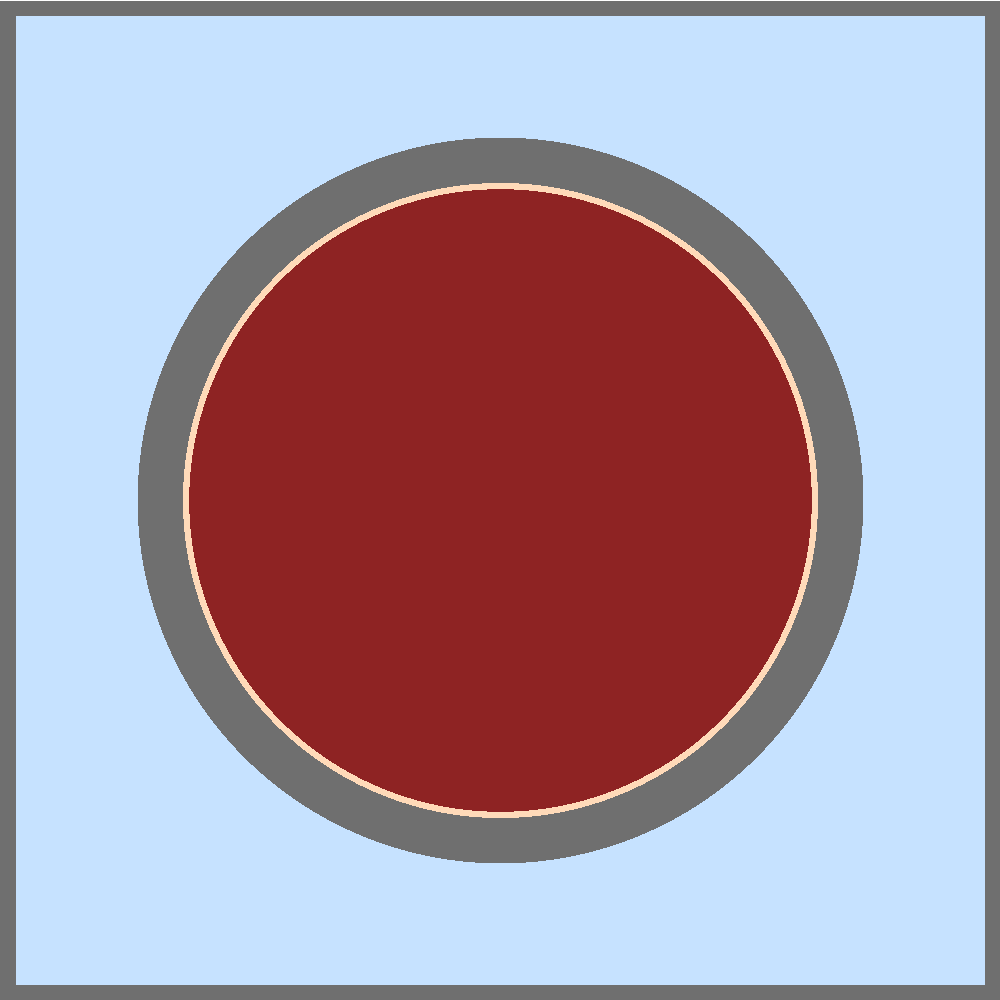
\includegraphics[width=0.9\linewidth]{figures/benchmarks/fuel-pin-16}
  \caption{}
  \label{fig:chap7-pin-1.6}
\end{subfigure}%
\begin{subfigure}{.5\textwidth}
  \centering
  
\includegraphics[width=0.9\linewidth]{figures/benchmarks/guide-tube}
  \caption{}
  \label{fig:chap7-pin-crgt}
\end{subfigure}
\begin{subfigure}{.5\textwidth}
  \centering
  
\includegraphics[width=0.9\linewidth]{figures/benchmarks/instr-tube}
  \caption{}
  \label{fig:chap7-instr-tube}
\end{subfigure}%
\begin{subfigure}{.5\textwidth}
  \centering
  \includegraphics[width=0.9\linewidth]{figures/benchmarks/burn-abs}
  \caption{}
  \label{fig:chap7-bp}
\end{subfigure}%
\caption[BEAVRS pin cell geometries]{1.6\% enriched fuel pin (a), control rod guide tube (b), instrument tube (c) and burnable poison (d). Light blue is borated water, red is UO$_2$ fuel, gray is zircaloy, brown is helium, white is air and green is borosolicate glass.}
\label{fig:chap7-pin-cells}
\end{figure}

%The radii for each material zone in the pin cells are detailed in Tab.~\ref{table:chap7-pin-cell-radii}. Each pin is surrounded by borated water and a zircaloy egg-crate grid spacer.  The pin cell pitch is 1.25984 cm and the thickness of the grid spacer is 0.02014 cm.

%\addtocounter{footnote}{-2}
%\stepcounter{footnote}\footnotetext{The control rod guide tube geometry above the dashpot.}
%\stepcounter{footnote}\footnotetext{The burnable poison geometry above the dashpot.}


%%%%%%%%%%%%%%%%%%%%%%%%%%%%
\subsection{Fuel Assemblies}
\label{subsec:chap7-fuel-assms}

%The first three benchmark models are based upon 2D models of individual fuel assemblies extracted from the full core \ac{BEAVRS} model. Each assembly consists of a 17$\times$17 rectilinear array of pin cells with a total height and width of 21.41728 cm. The stainless steel grid sleeve and water separating each fuel assembly in the full core \ac{BEAVRS} model are not included in the individual models of each fuel assembly. The intra-pin egg-crate grid spacer is included in each benchmark model. The assemblies are modeled with reflective \acp{BC} to simulate an infinite repeating lattice of each fuel assembly. 

The first three benchmark models are based upon 2D models of individual fuel assemblies extracted from the full core \ac{BEAVRS} model. Each assembly consists of a 17$\times$17 rectilinear array of pin cells with a total height and width of 21.41728 cm. The intra-pin egg-crate grid spacer and grid sleeve separating each fuel assembly in the full core \ac{BEAVRS} model are not included in the individual models of each fuel assembly. The assemblies are modeled with reflective \acp{BC} to simulate an infinite repeating lattice of each fuel assembly. 

\begin{figure}[h!]
  \centering
  \includegraphics[width=0.65\linewidth]{figures/benchmarks/assembly-16}
\vspace{2mm}
\caption[BEAVRS 1.6\% enriched assembly]{A 1.6\% enriched UO$_2$ fuel assembly without \acp{BP}.}
\label{fig:chap7-assm-16}
\end{figure}

\begin{figure}[h!]
  \centering
  \includegraphics[width=0.65\linewidth]{figures/benchmarks/assembly-31}
\vspace{2mm}
\caption[BEAVRS 3.1\% enriched assembly]{A 3.1\% enriched UO$_2$ fuel assembly without \acp{BP}.}
\label{fig:chap7-assm-31}
\end{figure}

\begin{figure}[h!]
  \centering
  \includegraphics[width=0.65\linewidth]{figures/benchmarks/assembly-31-20BPs}
\vspace{2mm}
\caption[BEAVRS 3.1\% enriched assembly with 20 BPs]{A 3.1\% enriched UO$_2$ fuel assembly with 20 \acp{BP}.}
\label{fig:chap7-assm-31-20BPs}
\end{figure}

The sequence of fuel assembly benchmarks are designed to investigate the impact of fuel enrichment, \acp{CRGT} and \acp{BP} on spatially self-shielded \ac{MGXS}. The first fuel assembly benchmark depicted in Fig.~\ref{fig:chap7-assm-16} consists of 264 fuel pins with 1.6\% enriched UO$_2$ fuel, 24 \acp{CRGT}, and a single central instrument tube. The second benchmark shown in Fig.~\ref{fig:chap7-assm-31} is of the same geometric configuration, but is composed of 3.1\% enriched UO$_2$ fuel. The third benchmark illustrated in Fig.~\ref{fig:chap7-assm-31-20BPs} includes 3.1\% enriched UO$_2$ fuel with a mixture of 20 \acp{BP}, 4 \acp{CRGT} and a single central instrument tube. Although the \ac{BEAVRS} model is composed of assemblies with many different \ac{BP} configurations, only a single assembly with \acp{BP} was studied for practical reasons.

%%%%%%%%%%%%%%%%%%%%%%%%%%%%%%%%%%%%%%
\subsection{2$\times$2 Assembly Colorsets}
\label{subsec:chap7-2x2-colorsets}

%Two benchmarks were constructed from 2$\times$2 colorsets of fuel assemblies from the \ac{BEAVRS} model presented in Sec.~\ref{subsec:chap7-fuel-assms}. The pitch between fuel assemblies in the colorsets is 21.41728 cm (the height/width of each assembly). The stainless steel grid sleeve and water separating each fuel assembly in the full core \ac{BEAVRS} model are not included in the 2$\times$2 colorsets. The intra-pin egg-crate grid spacer is included in each benchmark model. The first colorset is modeled with periodic \acp{BC} on all sides to simulate an infinitely repeating lattice of fuel assemblies. The second colorset is surrounded by a water reflector on the bottom and right that is of the same width as a fuel assembly. The reflected colorset does not include the stainless steel baffle surrounding the fuel assemblies adjacent to the water reflector in the full core \ac{BEAVRS} model. The reflected colorset includes reflective \acp{BC} on the top and left (adjacent to the fuel assemblies) with vacuum \acp{BC} on the bottom and right (adjacent to the reflector).

Two benchmarks were constructed from 2$\times$2 colorsets of fuel assemblies from the \ac{BEAVRS} model presented in Sec.~\ref{subsec:chap7-fuel-assms}. The pitch between fuel assemblies in the colorsets is 21.41728 cm (the height/width of each assembly). The intra-pin egg-crate grid spacer and grid sleeve separating each fuel assembly in the full core \ac{BEAVRS} model are not included in the 2$\times$2 colorsets. The first colorset is modeled with periodic \acp{BC} on all sides to simulate an infinitely repeating lattice of fuel assemblies. The second colorset is surrounded by a water reflector on the bottom and right that is of the same width as a fuel assembly. The reflected colorset does not include the stainless steel baffle surrounding the fuel assemblies adjacent to the water reflector in the full core \ac{BEAVRS} model. The reflected colorset includes reflective \acp{BC} on the top and left (adjacent to the fuel assemblies) with vacuum \acp{BC} on the bottom and right (adjacent to the reflector).

\begin{figure}[h!]
  \centering
  \includegraphics[width=0.63\linewidth]{figures/benchmarks/2x2}
\vspace{2mm}
\caption[A 2$\times$2 colorset of BEAVRS assemblies]{A 2$\times$2 colorset of BEAVRS assemblies with periodic BCs.}
\label{fig:chap7-2x2}
\end{figure}

\begin{figure}[h!]
  \centering
  \includegraphics[width=0.63\linewidth]{figures/benchmarks/reflector}
\vspace{2mm}
\caption[A reflected 2$\times$2 colorset of BEAVRS assemblies]{A 2$\times$2 colorset of BEAVRS assemblies surrounded by a water reflector. Reflective \acp{BC} were applied on the left/top, with vacuum \acp{BC} on the right/bottom.}
\label{fig:chap7-reflector}
\end{figure}

The first 2$\times$2 colorset model shown in Fig.~\ref{fig:chap7-2x2} is composed of a checkerboard pattern of the fuel assemblies of 1.6\% enriched UO$_2$ without \acp{BP} (Fig.~\ref{fig:chap7-assm-16}) and 3.1\% enriched UO$_2$ with 20 \acp{BP} (Fig.~\ref{fig:chap7-assm-31-20BPs}). The first colorset benchmark is designed to investigate the effects of inter-assembly spatial heterogeneities on the spatially self-shielded \ac{MGXS} of fuel pins of different enrichments (\textit{i.e.}, from different fuel assemblies) placed adjacent to one another. The second benchmark illustrated in Fig.~\ref{fig:chap7-reflector} is the same 2$\times$2 colorset of fuel assemblies, but is surrounded by a water reflector. This benchmark is designed to quantify the impact of the moderation provided by the reflector, as well as the leakage of neutrons through the reflector, on spatially self-shielded \ac{MGXS}.

%%%%%%%%%%%%%%%%%%%%%%%%%%%%%
\subsection{BEAVRS Quarter Core}
\label{subsec:chap7-full-core}

The sixth and final benchmark is a 2D planar slice of the top right quadrant of the quadrant symmetric \ac{BEAVRS} core model\footnote{The \ac{BEAVRS} model was made quadrant symmetric by replacing all instrument tubes with empty \acp{CRGT}.} at the axial mid-plane as shown in Fig.~\ref{fig:chap7-full-core}. The fuel assemblies in the model are configured according to the cycle 1 loading pattern detailed in the \ac{BEAVRS} specifications~\cite{horelik2013beavrs}. The quarter core model includes assemblies with 1.6\%, 2.4\% and 3.1\% enriched UO$_2$ fuel depicted as red, blue and yellow in Fig.~\ref{fig:chap7-full-core}, respectively. The benchmark model is the all rods out configuration with a critical boron concentration of 975 ppm~\cite{horelik2013beavrs}.

The intra-pin egg-crate grid spacer and grid sleeve separating each fuel assembly in the 3D core \ac{BEAVRS} model are not included in 2D model at the axial mid-plane. All other radial heterogeneities in the \ac{BEAVRS} specifications are included in this model, including the inter-assembly water gaps, stainless steel baffle surrounding the fuel assemblies, core barrel, neutron shield panels and pressure vessel. The space outside of the pressure vessel is filled with air with vacuum \acp{BC} applied to planar surfaces on the top, bottom, left and right. The 2D quarter core \ac{BEAVRS} model builds upon the preceding five simpler benchmarks to explore the impact of radial heterogeneities in a realistic core configuration on spatially self-shielded \ac{MGXS}.

\begin{figure}[h!]
  \centering
  \includegraphics[width=0.9\linewidth]{figures/benchmarks/quarter-core}
\vspace{2mm}
\caption[The 2D quarter core \ac{BEAVRS} model]{The 2D quarter core \ac{BEAVRS} model.}
\label{fig:chap7-full-core}
\end{figure}


%%%%%%%%%%%%%%%%%%%%%%%%%%%%%%%%%%%%%%%%%%%%%%%%%%%%%%%%%%%%%%%%%%%%%%%%%%%%%%%
\section{Reference Results}
\label{sec:chap7-ref-results}

This section presents the reference results computed using OpenMC for each of the six benchmarks presented in the preceding section. As discussed in Sec.~\ref{subsec:chap7-src-stationarity}, OpenMC was employed to compute the Shannon entropy to determine the number of batches of particle histories needed to reach source stationarity. Sec.~\ref{subsec:chap7-eigenvalues} presents the converged $k_{eff}$ eigenvalue computed by OpenMC for each of the six benchmarks. Finally, Sec.~\ref{subsec:chap7-pin-powers} and Sec.~\ref{subsec:chap7-capture-rates} present the reference pin-wise spatial distributions of fission rates and U-238 capture rates in each benchmark as tallied in OpenMC, along with the associated uncertainties and batch-wise convergence for each reference solution.

The ENDF/B-VII.1 continuous energy cross section libraries evaluated at 600K provided by the MCNP code~\cite{mcnpx2003manual} were used by OpenMC for all simulations. It should be noted that isotropic in lab scattering was employed for all reference calculations with OpenMC's iso-in-lab feature (see Sec.~\ref{subsec:chap4-iso-in-lab}). Although isotropic in lab scattering is a poor approximation for \acp{LWR}, it eliminated scattering source anisotropy as one possible cause of approximation error between OpenMC and OpenMOC\footnote{At the time of this writing, OpenMOC employed an isotropic in lab neutron scattering kernel.} in order to isolate approximation errors resulting from spatially self-shielded \ac{MGXS}.

The reference solutions for each assembly and colorset benchmark model was computed with 100 inactive and 900 active batches of 10$^7$ particle histories per batch. The reference solution for the quarter core \ac{BEAVRS} model was computed with 200 inactive and 800 active batches of 10$^8$ histories per batch. Each OpenMC simulation was performed in parallel on ten compute nodes on the Falcon supercomputer at Idaho National Laboratory. Each compute node contained two dual socket Intel Xeon E5-2680 CPUs with 12 cores and 132 gigabytes of DRAM\footnote{Dynamic Random Access Memory.}. Four MPI processes were launched on each node (two MPI processes per CPU) with 6 OpenMP parallel threads per MPI process.

%%%%%%%%%%%%%%%%%%%%%%%%%%%%%%%
\subsection{Source Stationarity}
\label{subsec:chap7-src-stationarity}

The first metric that was evaluated for each of the six benchmarks was the stationarity of the fission source distribution. The initial distribution of fission source sites is uniformly distributed in space across fissile material zones by OpenMC for the first batch of particle histories. Each subsequent batch of fission source sites is drawn from a bank of fission sites populated during the preceding batch of particle histories. In eigenvalue calculations, the distribution of fission source sites must reach stationarity before tallying integral quantities such as the eigenvalue or reaction rates. 

The Shannon entropy is a commonly used diagnostic to measure source stationarity in \ac{MC} eigenvalue calculations~\cite{brown2006entropy}. To compute the Shannon entropy, a mesh of $M$ mesh cells is superimposed across the geometry and the number of fission source cites in each mesh cell is tabulated. The empirical multinomial probabilities $p_{i}$ for fission source sites is computed for each mesh cell $i$ as the ratio of sites in that cell to the total number of source sites in the geometry. The Shannon entropy $H$ is then computed from the multinomial probability distribution from the following equation:

\begin{equation}
\label{eqn:chap7-shannon-entropy}
H = \displaystyle\sum\limits_{i=1}^{M} p_{i} \log_{2} p_{i}
\end{equation}

\noindent The Shannon entropy provides a single scalar value which characterizes the spatial distribution of fission source sites. By monitoring the value of $H$ for each batch, one may determine the number of inactive batches needed to reach source stationarity.

The Shannon entropy was computed using a rectilinear pin-wise mesh for each of the six benchmark models and plotted in Fig.~\ref{fig:chap7-entropy}. The entropies in the plot are normalized to the entropy at the final 1000$^{\text{th}}$ batch in order to standardize the entropies for comparison in the same plot. The entropies for each of the three fuel assembly benchmarks, as well as the 2$\times$2 colorset without a reflector, all lie very near unity and do not exhibit any convergence behavior in the plot. The entropy for the 2$\times$2 colorset with a reflector appears to converge to near unity within 30 batches. Finally, the entropy for the high dominance ratio \ac{BEAVRS} quarter core appears to converge within 200 batches. 

\begin{figure}[h!]
  \centering
  \includegraphics[width=0.7\linewidth]{figures/benchmarks/entropy/entropy-all}
\caption[Shannon entropy source convergence for BEAVRS geometries]{Shannon entropy source convergence for BEAVRS geometries.}
\label{fig:chap7-entropy}
\end{figure}

As expected, the number of batches required to reach source stationarity increases with the benchmark size and heterogeneity, and the corresponding increase in the dominance ratio. This analysis of the Shannon entropy for each benchmark was used to determine an appropriately conservative number of inactive batches to employ in all subsequent OpenMC simulations of each benchmark model. In particular, all OpenMC simulations of the single assembly and 2$\times$2 colorsets use 100 inactive batches prior to tallying the eigenvalue, reference reaction rate distributions and \ac{MGXS}. Similarly, 200 inactive batches are used for the quarter core \ac{BEAVRS} model.

%%%%%%%%%%%%%%%%%%%%%%%%
\subsection{Eigenvalues}
\label{subsec:chap7-eigenvalues}

The reference eigenvalues were computed for each of the six benchmarks and are listed in Tab.~\ref{table:chap7-ref-eigenvalues}. The OpenMC ``combined'' eigenvalue estimator is reported along with the associated one sigma uncertainty of 1 \ac{pcm} or less for each of the benchmarks. The total runtimes required for the OpenMC simulations to generate the reference eigenvalues are also reported in the table. 

%A total of 9,000,000,000 particle histories (900 active batches of 10$^7$ particle histories per batch) were simulated for the individual fuel assembly and 2$\times$2 colorset benchmarks, while 8,000,000,000 total particle histories (800 active batches) were simulated for the quarter core \ac{BEAVRS} model.

\begin{table}[h!]
  \centering
  \caption[Reference $k^{OpenMC}_{eff}$ for heterogeneous benchmarks]{Reference $k^{OpenMC}_{eff}$ for heterogeneous benchmarks.}
  \small
  \label{table:chap7-ref-eigenvalues}
  \vspace{6pt}
  \begin{tabular}{l C{4cm} r}
  \toprule
  \rowcolor{lightgray}
  \textbf{Benchmark} & $\bm{k^{OpenMC}_{eff}}$ & \textbf{Runtime [core-hours]} \\
  \midrule
  1.6\% Enriched Assembly (no \ac{BP}s) & 0.99326 $\pm$ 0.00001 & 1,005 \\
  3.1\% Enriched Assembly (no \ac{BP}s) & 1.21657 $\pm$ 0.00001 & 891 \\
  3.1\% Enriched Assembly (20 \ac{BP}s) & 1.03315 $\pm$ 0.00001 & 879 \\
  2$\times$2 Colorset & 1.01814 $\pm$ 0.00001 & 903 \\
  2$\times$2 Colorset w/ Reflector & 0.94574 $\pm$ 0.00001 & 895 \\
  \ac{BEAVRS} Quarter Core & 1.02446 $\pm$ 0.00000 & 10,892 \\
  \bottomrule
\end{tabular}
\end{table}

As expected, the eigenvalues increase with enrichment and decrease with the presence of \acp{BP} for the single fuel assembly benchmarks. The eigenvalue for the 2$\times$2 colorset is reduced with the addition of a reflector due to leakage, and to a lesser extent, absorption in the reflector. Although the quarter core \ac{BEAVRS} model is a critical configuration, the eigenvalue is nearly 2500 pcm supercritical due to the iso-in-lab scattering approximation\footnote{An identical OpenMC simulation of the  3D full core \ac{BEAVRS} model using normal anisotropic scattering produced an eigenvalue of 0.99922 $\pm$ 0.00000.}. The eigenvalues reported in Tab.~\ref{table:chap7-ref-eigenvalues} are used to validate the OpenMOC simulations with \ac{MGXS} generated by OpenMC throughout the following chapters.

%%%%%%%%%%%%%%%%%%%%%%%%%%%%%%%%%%%%
\subsection{Fission Rate Spatial Distributions}
\label{subsec:chap7-pin-powers}

The reference energy-integrated fission rate spatial distributions for each of the six benchmarks were computed using rectilinear, pin-wise tally meshes in OpenMC. The fission rates were volume-integrated across each fuel pin and include fission from all nuclides (only U-235 and U-238 for the fresh \ac{PWR} UO$_2$ fuel in the benchmarks). The fission rates were normalized to the mean of all non-zero fission rates in each benchmark. The percent relative errors for the tallied fission rates was computed from the ratio of the sample standard deviation to the mean fission rate in each fuel pin. The fission rates for the quarter core \ac{BEAVRS} model were appropriately tiled to display the equivalent distribution across the quadrant symmetric full core.

The fission rate spatial distributions and percent relative errors for each of the six benchmarks are presented as heatmaps in Figs.~\Crefrange{fig:chap7-fiss-rates-1.6-assm}{fig:chap7-fiss-rates-full-core}. The fission rates in the instrument tubes, \acp{CRGT} and \acp{BP} are all zero and are illustrated in white. The color bars for each of the heatmaps range from the minimum non-zero fission rate to the maximum fission rate for all fuel pins in each benchmark geometry. The statistical error at the final 1000$^{\text{th}}$ batch is less than or equal to 0.5\% for all of the benchmarks. These reference fission rate spatial distributions are used to validate the OpenMOC simulations with \ac{MGXS} generated by OpenMC throughout the following chapters.

%The batch-wise convergence rates of the fission rates is shown for the maximum and mean percent relative errors for each of the benchmarks in Fig.~\ref{fig:chap7-fiss-rates-conv}.

As illustrated in the figures, the fission rate distributions are strongly dependent on the spatially heterogeneous features in each benchmark geometry. For example, the \acp{CRGT} provide additional moderation and increase the fission rates in nearby fuel pins. The presence of \acp{BP} reduces the neutron population and therefore the fission rates for the surrounding fuel pins, while increasing the variation between the minimum and maximum fission rates. The presence of a reflector with a mixture of vacuum and reflective \acp{BC} induces a tilt in the fission rates across the assemblies in the 2$\times$2 colorset, with the maximum fission rates located in the interior fuel pins and the minimum fission rates occurring near the reflector due to neutron leakage. The fission rates for the quarter core \ac{BEAVRS} model in Fig.~\ref{fig:chap7-fiss-rates-full-core} form a highly complex spatial distribution due to the convolution of many different interacting spatial self-shielding effects.

It should be noted that the fission rate distribution for the quarter core \ac{BEAVRS} model is highly skewed due to the isotropic in lab scattering approximation. This can be seen from comparison of Fig.~\ref{fig:chap7-fiss-rate-mean-full-core} with the true fission rate distribution calculated with normal anisotropic scattering in Fig.~\ref{fig:benchmarks-beavrs-fiss-aniso}. The power distribution is highly sensitive to anisotropic scattering due to radial leakage out of the core, and is more peaked near the corner reflectors when the isotropic approximation is made. Although isotropic scattering is unphysical, it allows direct comparisons of OpenMC and OpenMOC results in latter chapters to quantify the impact of various approaches to spatially homogenize \ac{MGXS} without conflicting effects due to the isotropic scattering model used in OpenMOC.

\begin{figure}[h!]
\centering
\begin{subfigure}{0.44\textwidth}
  \centering
  \includegraphics[width=\linewidth]{figures/benchmarks/fission-rates/fiss-mean-assm-16}
  \caption{}
  \label{fig:chap7-fiss-rate-mean-1.6-assm}
\end{subfigure}%
\begin{subfigure}{0.44\textwidth}
  \centering
  \includegraphics[width=\linewidth]{figures/benchmarks/fission-rates/fiss-rel-err-assm-16}
  \caption{}
  \label{fig:chap7-fiss-rate-rel-err-1.6-assm}
\end{subfigure}%
\caption[Fission rates for a 1.6\% enriched assembly]{Fission rates for a 1.6\% enriched assembly.}
\label{fig:chap7-fiss-rates-1.6-assm}
\end{figure}

\begin{figure}[h!]
\centering
\begin{subfigure}{0.44\textwidth}
  \centering
  \includegraphics[width=\linewidth]{figures/benchmarks/fission-rates/fiss-mean-assm-31}
  \caption{}
  \label{fig:chap7-fiss-rate-mean-3.1-assm}
\end{subfigure}%
\begin{subfigure}{0.44\textwidth}
  \centering
  \includegraphics[width=\linewidth]{figures/benchmarks/fission-rates/fiss-rel-err-assm-31}
  \caption{}
  \label{fig:chap7-fiss-rate-rel-err-3.1-assm}
\end{subfigure}%
\caption[Fission rates for a 3.1\% enriched assembly]{Fission rates for a 3.1\% enriched assembly.}
\label{fig:chap7-fiss-rates-3.1-assm}
\end{figure}

\begin{figure}[h!]
\centering
\begin{subfigure}{0.44\textwidth}
  \centering
  \includegraphics[width=\linewidth]{figures/benchmarks/fission-rates/fiss-mean-assm-31-20BPs}
  \caption{}
  \label{fig:chap7-fiss-rate-mean-3.1-20BAs-assm}
\end{subfigure}%
\begin{subfigure}{0.44\textwidth}
  \centering
  \includegraphics[width=\linewidth]{figures/benchmarks/fission-rates/fiss-rel-err-assm-31-20BPs}
  \caption{}
  \label{fig:chap7-fiss-rate-rel-err-3.1-20BAs-assm}
\end{subfigure}%
\caption[Fission rates for a 3.1\% enriched assembly with 20 BPs]{Fission rates for a 3.1\% enriched assembly with 20 \ac{BP}s.}
\label{fig:chap7-fiss-rates-3.1-assm-20BAs}
\end{figure}

\begin{figure}[h!]
\centering
\begin{subfigure}{0.44\textwidth}
  \centering
  \includegraphics[width=\linewidth]{figures/benchmarks/fission-rates/fiss-mean-2x2}
  \caption{}
  \label{fig:chap7-fiss-rate-mean-2x2}
\end{subfigure}%
\begin{subfigure}{0.44\textwidth}
  \centering
  \includegraphics[width=\linewidth]{figures/benchmarks/fission-rates/fiss-rel-err-2x2}
  \caption{}
  \label{fig:chap7-fiss-rate-rel-err-2x2}
\end{subfigure}%
\caption[Fission rates for a 2$\times$2 colorset]{Fission rates for a 2$\times$2 colorset.}
\label{fig:chap7-fiss-rates-2x2}
\end{figure}

\begin{figure}[h!]
\centering
\begin{subfigure}{0.44\textwidth}
  \centering
  \includegraphics[width=\linewidth]{figures/benchmarks/fission-rates/fiss-mean-reflector}
  \caption{}
  \label{fig:chap7-fiss-rate-conv}
\end{subfigure}%
\begin{subfigure}{0.44\textwidth}
  \centering
  \includegraphics[width=\linewidth]{figures/benchmarks/fission-rates/fiss-rel-err-reflector}
  \caption{}
  \label{fig:chap7-fiss-rate-conv}
\end{subfigure}%
\caption[Fission rates for a 2$\times$2 colorset with a reflector]{Fission rates for a 2$\times$2 colorset with a reflector.}
\label{fig:chap7-fiss-rates-reflector}
\end{figure}

\begin{figure}[h!]
\centering
\begin{subfigure}{0.44\textwidth}
  \centering
  \includegraphics[width=\linewidth]{figures/benchmarks/fission-rates/fiss-mean-full-core}
  \caption{}
  \label{fig:chap7-fiss-rate-mean-full-core}
\end{subfigure}%
\begin{subfigure}{0.44\textwidth}
  \centering
  \includegraphics[width=\linewidth]{figures/benchmarks/fission-rates/fiss-rel-err-full-core}
  \caption{}
  \label{fig:chap7-fiss-rate-rel-err-full-core}
\end{subfigure}%
\caption[Fission rates for the full 2D BEAVRS core]{Fission rates for the 2D quarter core \ac{BEAVRS} model.}
\label{fig:chap7-fiss-rates-full-core}
\end{figure}

%\begin{figure}[h!]
%\centering
%\begin{subfigure}{\textwidth}
%  \centering
%  \includegraphics[width=0.8\linewidth]{figures/benchmarks/fission-rates/fiss-conv-max-assms}
%  \caption{}
%  \label{fig:chap7-fiss-rate-max-conv-max}
%\end{subfigure}
%\begin{subfigure}{\textwidth}
%  \centering
%  \includegraphics[width=0.8\linewidth]{figures/benchmarks/fission-rates/fiss-conv-mean-assms}
%  \caption{}
%  \label{fig:chap7-fiss-rate-max-conv-mean}
%\end{subfigure}
%\caption[Fission rate relative error convergence for BEAVRS geometries]{The maximum (a) and mean (b) fission rate relative error convergence for the six heterogeneous benchmark geometries.}
%\label{fig:chap7-fiss-rates-conv}
%\end{figure}

\clearpage

%%%%%%%%%%%%%%%%%%%%%%%%%%%%%%%%%%%%%%%%%%%%%
\subsection{U-238 Capture Rate Spatial Distributions}
\label{subsec:chap7-capture-rates}

The reference energy-integrated U-238 capture rate spatial distributions for each of the six benchmarks were computed using rectilinear, pin-wise tally meshes in OpenMC. The U-238 capture rates were volume-integrated across each fuel pin. The capture rates were normalized to the mean of all non-zero capture rates in each benchmark. The percent relative errors for the tallied capture rates was computed from the ratio of the sample standard deviation to the mean capture rate in each fuel pin. The capture rates for the quarter core \ac{BEAVRS} model were appropriately tiled to display the equivalent distribution across the quadrant symmetric full core.

The U-238 capture rate spatial distributions and percent relative errors for each of the six benchmarks are presented as heatmaps in Figs.~\Crefrange{fig:chap7-capt-rates-1.6-assm}{fig:chap7-capt-rates-full-core}. The capture rates in the instrument tubes, \acp{CRGT} and \acp{BP} are all zero and are illustrated in white. The color bars for each of the heatmaps range from the minimum non-zero capture rate to the maximum capture rate for all fuel pins in each benchmark geometry. The maximum relative error at the final 1000$^{\text{th}}$ batch is less than 0.5\% for all of the benchmarks. These reference U-238 capture rate spatial distributions are used to validate the OpenMOC simulations with \ac{MGXS} generated by from OpenMC throughout the following chapters.

%The batch-wise convergence rates of the capture rates is shown for the maximum and mean percent relative errors for each of the benchmarks in Fig.~\ref{fig:chap7-capt-rates-conv}.

The impacts of \acp{CRGT}, \acp{BP}, reflectors and vacuum \acp{BC} on the U-238 capture rates are similar to those observed for the fission rates, though there are some noticeable differences. For example, the U-238 capture rates in the individual fuel assemblies appear to be more sensitive than the fission rates to the spatial self-shielding induced by moderation in \acp{CRGT}. In addition, the U-238 capture rates peak in the 1.6\% enriched fuel assemblies in the 2$\times$2 colorset without a reflector (Fig.~\ref{fig:chap7-capt-rate-rel-err-2x2}), while the fission rates peak in the 3.1\% enriched fuel assemblies (Fig.~\ref{fig:chap7-fiss-rate-rel-err-2x2}). The key reason for this is that there is a higher concentration of U-238 in the 1.6\% enriched fuel than the 3.1\% enriched fuel, which leads to a lower ratio of fission to U-238 capture rates. In addition, the U-238 capture rates in the reflected 2$\times$2 benchmark (Fig.~\ref{fig:chap7-capt-rates-reflector}) are more smoothly varying at the inter-assembly interface than the fission rates (Fig.~\ref{fig:chap7-fiss-rates-reflector}).

\begin{figure}[h!]
\centering
\begin{subfigure}{0.44\textwidth}
  \centering
  \includegraphics[width=\linewidth]{figures/benchmarks/capture-rates/capt-mean-assm-16}
  \caption{}
  \label{fig:chap7-capt-rate-mean-1.6-assm}
\end{subfigure}%
\begin{subfigure}{0.44\textwidth}
  \centering
  \includegraphics[width=\linewidth]{figures/benchmarks/capture-rates/capt-rel-err-assm-16}
  \caption{}
  \label{fig:chap7-capt-rate-rel-err-1.6-assm}
\end{subfigure}%
\caption[U-238 capture rates for a 1.6\% enriched assembly]{U-238 capture rates for a 1.6\% enriched assembly.}
\label{fig:chap7-capt-rates-1.6-assm}
\end{figure}

\begin{figure}[h!]
\centering
\begin{subfigure}{0.44\textwidth}
  \centering
  \includegraphics[width=\linewidth]{figures/benchmarks/capture-rates/capt-mean-assm-31}
  \caption{}
  \label{fig:chap7-capt-rate-mean-3.1-assm}
\end{subfigure}%
\begin{subfigure}{0.44\textwidth}
  \centering
  \includegraphics[width=\linewidth]{figures/benchmarks/capture-rates/capt-rel-err-assm-31}
  \caption{}
  \label{fig:chap7-capt-rate-rel-err-3.1-assm}
\end{subfigure}%
\caption[U-238 capture rates for a 3.1\% enriched assembly]{U-238 capture rates for a 3.1\% enriched assembly.}
\label{fig:chap7-capt-rates-3.1-assm}
\end{figure}

\begin{figure}[h!]
\centering
\begin{subfigure}{0.44\textwidth}
  \centering
  \includegraphics[width=\linewidth]{figures/benchmarks/capture-rates/capt-mean-assm-31-20BPs}
  \caption{}
  \label{fig:chap7-capt-rate-mean-3.1-20BAs-assm}
\end{subfigure}%
\begin{subfigure}{0.44\textwidth}
  \centering
  \includegraphics[width=\linewidth]{figures/benchmarks/capture-rates/capt-rel-err-assm-31-20BPs}
  \caption{}
  \label{fig:chap7-capt-rate-rel-err-3.1-20BAs-assm}
\end{subfigure}%
\caption[U-238 capture rates for a 3.1\% enriched assembly with 20 BPs]{U-238 capture rates for a 3.1\% enriched assembly with 20 \ac{BP}s.}
\label{fig:chap7-capt-rates-3.1-assm-20BAs}
\end{figure}

\begin{figure}[h!]
\centering
\begin{subfigure}{0.44\textwidth}
  \centering
  \includegraphics[width=\linewidth]{figures/benchmarks/capture-rates/capt-mean-2x2}
  \caption{}
  \label{fig:chap7-capt-rate-mean-2x2}
\end{subfigure}%
\begin{subfigure}{0.44\textwidth}
  \centering
  \includegraphics[width=\linewidth]{figures/benchmarks/capture-rates/capt-rel-err-2x2}
  \caption{}
  \label{fig:chap7-capt-rate-rel-err-2x2}
\end{subfigure}%
\caption[U-238 capture rates for a 2$\times$2 colorset]{U-238 capture rates for a 2$\times$2 colorset.}
\label{fig:chap7-capt-rates-2x2}
\end{figure}

\begin{figure}[h!]
\centering
\begin{subfigure}{0.44\textwidth}
  \centering
  \includegraphics[width=\linewidth]{figures/benchmarks/capture-rates/capt-mean-reflector}
  \caption{}
  \label{fig:chap7-capt-rate-mean-reflector}
\end{subfigure}%
\begin{subfigure}{0.44\textwidth}
  \centering
  \includegraphics[width=\linewidth]{figures/benchmarks/capture-rates/capt-rel-err-reflector}
  \caption{}
  \label{fig:chap7-capt-rate-rel-err-reflector}
\end{subfigure}%
\caption[U-238 capture rates for a 2$\times$2 colorset with a reflector]{U-238 capture rates for a 2$\times$2 colorset with a reflector.}
\label{fig:chap7-capt-rates-reflector}
\end{figure}

\begin{figure}[h!]
\centering
\begin{subfigure}{0.44\textwidth}
  \centering
  \includegraphics[width=\linewidth]{figures/benchmarks/capture-rates/capt-mean-full-core}
  \caption{}
  \label{fig:chap7-capt-rate-mean-full-core}
\end{subfigure}%
\begin{subfigure}{0.44\textwidth}
  \centering
  \includegraphics[width=\linewidth]{figures/benchmarks/capture-rates/capt-rel-err-full-core}
  \caption{}
  \label{fig:chap7-capt-rate-rel-err-full-core}
\end{subfigure}%
\caption[U-238 capture rates for the full 2D BEAVRS core]{U-238 capture rates for the 2D quarter core \ac{BEAVRS} model.}
\label{fig:chap7-capt-rates-full-core}
\end{figure}

Similar to the fission rates, the U-238 capture rate distribution for the quarter core \ac{BEAVRS} model is highly skewed due to the isotropic in lab scattering approximation. This can be seen from comparison of Fig.~\ref{fig:chap7-capt-rate-mean-full-core} with the true capture rate distribution calculated with normal anisotropic scattering in Fig.~\ref{fig:benchmarks-beavrs-capt-aniso}. Like fission, the U-238 capture distribution is highly sensitive to anisotropic scattering due to radial leakage out of the core, and is more peaked near the corner reflectors when the isotropic approximation is made. Although isotropic scattering is unphysical, it allows direct comparisons of OpenMC and OpenMOC results in latter chapters to quantify the impact of various approaches to spatially homogenize \ac{MGXS} without conflicting effects due to the isotropic scattering model used in OpenMOC.

%\begin{figure}[h!]
%\centering
%\begin{subfigure}{\textwidth}
%  \centering
%  \includegraphics[width=0.8\linewidth]{figures/benchmarks/capture-rates/capt-conv-max-assms}
%  \caption{}
%  \label{fig:chap7-capt-rate-max-conv}
%\end{subfigure}
%\begin{subfigure}{\textwidth}
%  \centering
%  \includegraphics[width=0.8\linewidth]{figures/benchmarks/capture-rates/capt-conv-mean-assms}
%  \caption{}
%  \label{fig:chap7-capt-rate-max-conv}
%\end{subfigure}
%\caption[U-238 capture rate relative error convergence for BEAVRS geometries]{The maximum (a) and mean (b) U-238 capture rate percent relative error convergence for the six heterogeneous benchmark geometries.}
%\label{fig:chap7-capt-rates-conv}
%\end{figure}

%\clearpage

\vfill
\begin{highlightsbox}[frametitle=Highlights]
\begin{itemize}
  \item A series of six 2D heterogeneous benchmark models were derived from the full core \ac{BEAVRS} model to explore spatial self-shielding effects on \ac{MGXS}.
  \item The benchmarks include individual fuel assemblies with different \ac{CRGT} and \ac{BP} configurations, 2$\times$2 fuel assembly colorsets with and without a water reflector, and the quarter core \ac{BEAVRS} model.
  \item The Shannon entropy was computed to determine the number of inactive batches needed when modeling each benchmark with OpenMC.
  \item Reference results for the eigenvalues, pin-wise fission rates and pin-wise U-238 capture rates were computed using OpenMC.
  \item The benchmarks and reference results are used in the following chapters to validate the use of statistical clustering methods to capture spatial self-shielding effects in \ac{MGXS} generated by OpenMC for OpenMOC.
\end{itemize}
\end{highlightsbox}
\vfill
\chapter{Quantification of Spatial Self-Shielding Effects}
\label{chap:quantify}


%%%%%%%%%%%%%%%%%%%%%%%%%%%%%%%%%%%%%%%%%%%%%%%%%%%%%%%%%%%%%%%%%%%%%%%%%%%%%%%
\section{Overview}
\label{sec:chap8-overview}

The preceding chapter introduced six heterogeneous 2D \ac{PWR} benchmarks derived from the \ac{BEAVRS} model, along with reference metrics tallied by OpenMC. This chapter applies multi-group transport calculations to model the same benchmarks in OpenMOC with \ac{MGXS} generated by OpenMC. The objective is to identify the bias between OpenMC and OpenMOC for \ac{MGXS} libraries which account for spatial self-shielding effects\footnote{The effects of neighboring pins, burnable poisons, reflectors and the core baffle, barrel and vessel are all of interest in the context of spatial self-shielding in this and subsequent chapters.} to varying degrees. In particular, this chapter quantifies the difference in the approximation error between simulations in which the same \ac{MGXS} are used in each unique fuel pin (\textit{e.g.}, each fuel enrichment) and those in which unique \ac{MGXS} are used in each and every pin. The former case does little if anything to model spatial self-shielding effects, whereas the latter case ``fully'' resolves these effects, albeit at the expense of very large \ac{MGXS} libraries. This difference in approximation error motivates the development of a novel methodology in the following chapters which uses statistical clustering to capture spatial self-shielding effects in \ac{MGXS}.

Three different schemes for spatial homogenization of pin-wise \ac{MGXS} are introduced in Sec.~\ref{sec:chap8-pinwise-space-homogenize} and are referred to as \textit{infinite}, \textit{null} and \textit{degenerate} spatial homogenization, respectively. The discretized models and runtime parameters used in the OpenMOC simulations are detailed in Sec.~\ref{sec:chap8-moc-params}. The bias between the OpenMOC simulations and the reference OpenMC results -- including eigenvalues, pin-wise fission rates and pin-wise U-238 capture rates -- are presented in Sec.~\ref{sec:chap8-mg-results}. The need for a new, more flexible and specialized approach to spatial homogenization which appropriately captures spatial self-shielding effects with minimal computational expense is discussed in Sec.~\ref{sec:chap8-motivate}.


%%%%%%%%%%%%%%%%%%%%%%%%%%%%%%%%%%%%%%%%%%%%%%%%%%%%%%%%%%%%%%%%%%%%%%%%%%%%%%%
\section{Pin-wise Spatial Homogenization Schemes}
\label{sec:chap8-pinwise-space-homogenize}

This chapter employs three different spatial homogenization schemes to model spatial self-shielding effects in \ac{MGXS}. Although all spatial zones may experience spatial self-shielding, this chapter only models the impact of spatial self-shielding on \ac{MGXS} in fissile regions. The infinite, null and degenerate spatial homogenization schemes are introduced in Secs.~\Crefrange{subsec:chap8-infinite}{subsec:chap8-degenerate}. These schemes model spatial self-shielding for each fuel pin with increasing granularity and complexity. The total number of materials (\textit{i.e.}, \ac{MGXS}) used to model each benchmark with each homogenization scheme is given in Tab.~\ref{table:chap8-num-materials}. A fuel assembly, 2$\times$2 colorset and part of the quarter core \ac{BEAVRS} model are color-coded by material and illustrated in Fig.~\ref{fig:chap8-homogenization-schemes} for each homogenization scheme.

The \texttt{openmc.mgxs} module (see Sec.~\ref{subsec:chap4-mgxs}) was used to compute 70-group \ac{MGXS} with OpenMC for each of the six heterogeneous benchmarks introduced in Chap.~\ref{chap:benchmarks}. The tallied \ac{MGXS} data was condensed to coarse 2-group and 8-group structures with downstream data processing as necessary. The OpenMC simulations were performed with 1000 batches with 10$^{6}$ particle histories per batch for each benchmark. This was only one tenth of the 10$^7$ histories per batch used to tally the reference results in Chap.~\ref{chap:benchmarks} for practical computational reasons\footnote{The total runtime consumed by OpenMC scales with the number of tallied quantities. The number of tallies used to compute \ac{MGXS} was much larger than the three used to compute the reference solutions in Chap.~\ref{chap:benchmarks}. As a result, the simulation time per history was prohibitively slow to generate \ac{MGXS} with the same number of histories as was used to compute the reference solution.}. Stationarity of the fission source was obtained with 200 inactive batches for the quarter core \ac{BEAVRS} model, while 100 inactive batches were employed for the other five benchmarks (see Sec.~\ref{subsec:chap7-src-stationarity}). OpenMC's ``iso-in-lab'' feature (see Sec.~\ref{subsec:chap4-iso-in-lab}) was employed to enable consistent comparisons between OpenMC's reference results and OpenMOC's calculations with an isotropic in lab scattering source.

\vspace{0.2in}

\begin{table}[h!]
  \centering
  \caption[Number of materials for each spatial homogenization scheme]{Number of materials modeled with unique \ac{MGXS} in each heterogeneous benchmark for each spatial homogenization scheme.}
  \small
  \label{table:chap8-num-materials}
  \vspace{6pt}
  \begin{tabular}{l r r r}
  \toprule
  \rowcolor{lightgray}
  & \multicolumn{3}{c}{\cellcolor{lightgray} \bf \# Fuel Materials} \\
  \multirow{-2}{*}{\cellcolor{lightgray} \bf Benchmark} &
  \multicolumn{1}{c}{\cellcolor{lightgray} \bf Infinite} &
  \multicolumn{1}{c}{\cellcolor{lightgray} \bf Null} &
  \multicolumn{1}{c}{\cellcolor{lightgray} \bf Degenerate} \\
  \midrule
1.6\% Assm & 1 & 1 & 264 \\
%1.6\% Assm & 5 & 5 & 268 \\
  \midrule
3.1\% Assm & 1 & 1 & 264 \\
%3.1\% Assm & 5 & 5 & 268 \\
  \midrule
3.1\% Assm w/ 20 BPs & 1 & 1 & 264  \\
%3.1\% Assm w/ 20 BPs & 7 & 7 & 270  \\
  \midrule
2$\times$2 Colorset & 2 & 2 & 1,056 \\
%2$\times$2 Colorset & 8 & 8 & 1,062 \\
  \midrule
2$\times$2 Colorset w/ Reflector & 2 & 2 & 1,056 \\
%2$\times$2 Colorset w/ Reflector & 8 & 8 & 1,062 \\
  \midrule
\ac{BEAVRS} Quarter Core & 3 & 3 & 12,993 \\ % 193 * 264 / 4. + 128 + 127 + 7 % 50,964
%\ac{BEAVRS} Quarter Core & 10 & 10 & 13,000 \\ % 193 * 264 / 4. + 128 + 127 + 7 % 50,964
  \bottomrule
\end{tabular}
\end{table}

\begin{figure}[h!]
\centering
\begin{subfigure}{.45\textwidth}
  \centering
  \includegraphics[width=0.87\linewidth]{figures/quantification/homogenization/assm-16-null-materials}
  \caption{}
  \label{fig:chap8-assm-16-null-materials}
\end{subfigure}%
\begin{subfigure}{.45\textwidth}
  \centering
  \includegraphics[width=0.87\linewidth]{figures/quantification/homogenization/assm-16-degenerate-materials}
  \caption{}
  \label{fig:chap8-assm-16-degenerate-materials}
\end{subfigure}
\begin{subfigure}{.45\textwidth}
  \centering
  \includegraphics[width=0.87\linewidth]{figures/quantification/homogenization/2x2-null-materials}
  \caption{}
  \label{fig:chap8-2x2-null-materials}
\end{subfigure}%
\begin{subfigure}{.45\textwidth}
  \centering
  \includegraphics[width=0.87\linewidth]{figures/quantification/homogenization/2x2-degenerate-materials}
  \caption{}
  \label{fig:chap8-2x2-degenerate-materials}
\end{subfigure}
\begin{subfigure}{.45\textwidth}
  \centering
  \includegraphics[width=0.87\linewidth]{figures/quantification/homogenization/full-core-null-materials}
  \caption{}
  \label{fig:chap8-full-core-null-materials}
\end{subfigure}%
\begin{subfigure}{.45\textwidth}
  \centering
  \includegraphics[width=0.87\linewidth]{figures/quantification/homogenization/full-core-degenerate-materials}
  \caption{}
  \label{fig:chap8-full-core-degenerate-materials}
\end{subfigure}
\caption[Depiction of infinite, null and degenerate spatial homogenization schemes]{OpenMOC materials for a single fuel assembly, a 2$\times$2 colorset and part of the 2D quarter core \ac{BEAVRS} model. The materials for the infinite and null schemes are depicted in (a), (c) and (e), and for the degenerate scheme in (b), (d) and (f), respectively. Each uniquely colored material represents a unique set of \ac{MGXS}.}
\label{fig:chap8-homogenization-schemes}
\end{figure}

%%%%%%%%%%%%%%%%%%%%%%%%%%%%%%%%%%%%%%
\subsection{Infinite Lattice Homogenization}
\label{subsec:chap8-infinite}

The \textit{infinite} spatial homogenization scheme is most reminiscent of the traditional multi-level schemes used to generate \ac{MGXS} (see Sec.~\ref{subsec:chap2-mgxs-lib-std-approach}), and is the simplest approach to model spatial self-shielding effects considered by this thesis. The infinite scheme employs multiple OpenMC simulations to compute \ac{MGXS} for each heterogeneous benchmark. The \ac{MGXS} for each type of fuel (\textit{e.g.}, enrichment) are generated by OpenMC simulations of each fuel pin type in an infinite, repeating array\footnote{An infinite, repeating array of fuel pins is modeled by a single fuel pin with reflective boundary conditions.}. The \ac{MGXS} for all other materials -- including borated water, zircaloy, helium, etc. -- are generated from OpenMC simulations of each heterogeneous benchmark where the reaction rates and fluxes are averaged across each geometry.

The infinite scheme is designed to quantify the impact of using the ``true'' Monte Carlo flux from an infinite lattice calculation, rather than the ``true'' \ac{MC} flux from the true heterogeneous geometry, to collapse \ac{MGXS} in fissile zones. The scheme employs a single \ac{MGXS} in each instance of a material zone, such as a fuel pin replicated many times throughout a benchmark geometry. The \ac{MGXS} for each fissile zone is generated from an infinite lattice calculation with OpenMC. The \ac{MGXS} for all non-fissile zones are generated using the ``true''  flux distribution in space and energy for each of the heterogeneous benchmarks. The scheme does not account for spatial self-shielding effects experienced by different non-fissile spatial zones filled by the same material, and instead averages these effects across the entire geometry for each material.

%-foonote: unable to run infinite pin cell calculations for non-fissile pin cells (CRGTs, BPs, instr tubes) since it's not a criticality calculation

%%%%%%%%%%%%%%%%%%%%%%%%%%%%%%%%%%%%%%
\subsection{Null Homogenization}
\label{subsec:chap8-null}

The \textit{null} spatial homogenization scheme builds upon the infinite scheme, but uses the ``true'' heterogeneous flux to collapse \ac{MGXS} for fissile as well as non-fissile materials. The null scheme eliminates the infinite lattice calculation to generate \ac{MGXS} for fissile zones, and instead uses a single Monte Carlo calculation of the complete heterogeneous geometry to generate \ac{MGXS} for \textit{all} materials. In this way, the null scheme fully abandons the multi-level approach used by the infinite scheme and most traditional approaches to generate \ac{MGXS}. Unlike the infinite scheme, the spatially self-shielded flux is used to collapse the cross sections in the fuel. However, the null scheme does not account for spatial self-shielding effects experienced by different fuel pins filled by the same type of fuel, and instead averages these effects across the entire geometry. As with the infinite scheme, a single \ac{MGXS} is employed in each instance of a material zone, such as a fuel pin replicated many times throughout a benchmark geometry.

%%%%%%%%%%%%%%%%%%%%%%%%%%%%%%%%%%%%%%
\subsection{Degenerate Homogenization}
\label{subsec:chap8-degenerate}

Unlike the infinite and null spatial homogenization schemes, the \textit{degenerate} scheme accounts for the different spatial self-shielding effects experienced by each instance of each fuel pin throughout a heterogeneous geometry. Like the null scheme, a single \ac{MC} calculation of the complete heterogeneous geometry is used to generate \ac{MGXS} for all materials. Unlike the null scheme, the \ac{MGXS} are tallied separately for each instance of fissile material zones. For example, if a heterogeneous benchmark includes $N$ fuel pins, then $N$ collections of \ac{MGXS} are separately tabulated for each fuel pin instance. The degenerate scheme tallies different \ac{MGXS} even if the isotopic compositions in the fuel pin instances are identical (\textit{e.g.}, fresh fuel at the beginning of life) since each instance may experience different spatial self-shielding effects and hence have different \ac{MGXS}.

Multi-group transport calculations with \ac{MGXS} generated using infinite/null and degenerate schemes may be compared to quantify the impact of modeling spatial self-shielding effects in \ac{MGXS} for fissile zones in heterogeneous geometries. The degenerate scheme applies the finest granularity to pin-wise spatial homogenization of any of the schemes considered in this thesis since it best captures different spatial self-shielding effects in each fuel pin. As a result, the degenerate scheme is used to benchmark the efficacy of the new methodology for spatial homogenization based on statistical clustering developed in the following chapters. Like both the infinite and null schemes, the spatial self-shielding effects experienced by different non-fissile spatial zones are averaged across the entire geometry for each non-fissile material.

The degenerate scheme generates \ac{MGXS} for each fuel pin instance using OpenMC's distributed cell tallies (see Sec.~\ref{subsec:chap4-distribcells}). The OpenCG region differentiation algorithm (see Sec.~\ref{sec:chap4-region-diff}) is used to build a new OpenMOC geometry with unique cells and materials for each fuel pin. The \ac{MGXS} are appropriately selected from OpenMC's distributed cell tallies to populate the \ac{MGXS} in the OpenMOC materials.

\begin{emphbox}
\textbf{The infinite, null and degenerate spatial homogenization schemes are used to quantify approximation errors made when neglecting spatial self-shielding due to neighboring pins, reflectors, etc. in heterogeneous \ac{PWR} benchmarks.}
\end{emphbox}


%%%%%%%%%%%%%%%%%%%%%%%%%%%%%%%%%%%%%%%%%%%%%%%%%%%%%%%%%%%%%%%%%%%%%%%%%%%%%%%
\section{\ac{MOC} Runtime Parameters}
\label{sec:chap8-moc-params}

The infinite, null and spatial homogenization schemes were used to prepare \ac{MGXS} libraries for OpenMOC simulations of each of the six heterogeneous \ac{PWR} benchmarks introduced in Chap.~\ref{chap:benchmarks}. This section briefly outlines the energy group structures and angular, spatial and \ac{CMFD} meshes used in the OpenMOC simulations. The total number of flat source regions, and \ac{MOC} tracks and segments are summarized for each benchmark in Tab.~\ref{table:chap8-num-fsrs-tracks-segments}. It was crucial to use an adequate discretization to accurately compare simulation results between the three spatial homogenization schemes, as well as to the reference OpenMC results.

\begin{table}[h!]
  \centering
  \caption[Number of \ac{FSR}s, tracks and segments for each heterogeneous benchmark]{The number of \ac{MOC} \ac{FSR}s, tracks and segments modeled in each benchmark.}
  \small
  \label{table:chap8-num-fsrs-tracks-segments}
  \vspace{6pt}
  \begin{tabular}{l r r r}
  \toprule
  \rowcolor{lightgray}
  \textbf{Benchmark} &
  \multicolumn{1}{c}{\cellcolor{lightgray} \textbf{\# \ac{FSR}s}} &
  \multicolumn{1}{c}{\cellcolor{lightgray} \textbf{\# Tracks}} &
  \multicolumn{1}{c}{\cellcolor{lightgray} \textbf{\# Segments}} \\
  \midrule
1.6\% Assm & 28,376 & 34,976 & 7,945,952 \\
  \midrule
3.1\% Assm & 28,376 & 34,976 & 7,945,952 \\
  \midrule
3.1\% Assm w/ 20 BPs & 29,496 & 34,976 & 8,110,192  \\
  \midrule
2$\times$2 Colorset & 115,744 & 69,892 & 32,097,936 \\
  \midrule
2$\times$2 Colorset w/ Reflector & 203,220 & 104,788 & 51,122,228 \\
  \midrule
%\ac{BEAVRS} Quarter Core & 2,512,384 & 201,620 & 427,683,579 \\
\ac{BEAVRS} Quarter Core & 1,718,368 & 201,620 & 38,3785,515 \\
  \bottomrule
\end{tabular}
\end{table}

Each simulation was converged to 10$^{-5}$ on the root mean square of the energy-integrated fission source in each flat source region (FSR). It should be noted that a convergence criterion of 10$^{-7}$ was employed for the OpenMOC simulations of simple benchmarks without \ac{CMFD} acceleration (see Sec.~\ref{subsubsec:chap4-openmoc-cmfd}) in Chap.~\ref{chap:biases}, but a looser convergence criterion of 10$^{-5}$ may be used for calculations with \ac{CMFD}\footnote{The convergence criterion measures the residual between successive iterations, but should actually measure convergence to the asymptotic solution, which depends on both the residual between successive iterations and the dominance ratio. \ac{CMFD} significantly reduces the residual between successive iterations such that sufficient convergence to the asymptotic solution is achieved at a much lower successive iteration residual.}.

%%%%%%%%%%%%%%%%%%%%%%%%%%%%%%%%%%%%
\subsection{Energy Group Structures}
\label{subsec:chap8-energy-groups}

Each assembly, colorset and quarter core benchmark was modeled with \ac{MGXS} in 2, 8 and 70 energy groups. The energy group structures were the same as those used in Chaps.~\ref{chap:biases} and~\ref{chap:sph} and are tabulated in App.~\ref{app:energy-groups}. The \ac{MOC} energy group structures were collapsed onto coarser group structures for \ac{CMFD} acceleration. The mapping from \ac{MOC} to \ac{CMFD} group structures is listed in Tab.~\ref{table:chap8-coarse-cmfd-groups}. The coarse \ac{CMFD} structures were derived to best approximate equal lethargy spacing between coarse \ac{CMFD} groups. The coarse \ac{CMFD} structures significantly improved the speed of the 70-group OpenMOC calculations.

\begin{table}[h!]
  \centering
  \caption[Coarse \ac{CMFD} group structures]{The coarse \ac{CMFD} group structures for each of the fine \ac{MOC} group structures.}
  \small
  \label{table:chap8-coarse-cmfd-groups}
  \vspace{6pt}
  \begin{tabular}{p{1.5cm} p{1.5cm} p{7.2cm}}
  \toprule
  \rowcolor{lightgray}
  \multicolumn{1}{c}{\cellcolor{lightgray} \textbf{\# \ac{MOC} Groups}} &
  \multicolumn{1}{c}{\cellcolor{lightgray} \textbf{\# \ac{CMFD} Groups}} &
  \multicolumn{1}{c}{\cellcolor{lightgray} \textbf{\ac{CMFD} Fine-to-Coarse Group Mapping}} \\
  \midrule
  \multicolumn{1}{c}{2} & \multicolumn{1}{c}{2} & [1], [2] \\
  \midrule
  \multicolumn{1}{c}{8} & \multicolumn{1}{c}{4} & [1--2], [3], [4--5], [6--8] \\
  \midrule
%  \multicolumn{1}{c}{40} & \multicolumn{1}{c}{10} & [1--3], [4--7], [8], [9], [10], [11--13], \hspace{0.8cm} [14--16], [17--29], [30--36], [37--40] \\
%  \midrule
  \multicolumn{1}{c}{70} & \multicolumn{1}{c}{14} & [1--2], [3--6], [7--9], [10--12], [13--16], \hspace{0.6cm} [17--19], [20--21], [22--24], [25--27], [28--33], [34--53], [54--61], [62--68], [69--70] \\ 
  \bottomrule
\end{tabular}
\end{table}

%%%%%%%%%%%%%%%%%%%%%%%%%%%%%%%%%%%%
\subsection{Angular Discretization}
\label{subsec:chap8-angular-discretizations}

The OpenMOC simulations of each of the six heterogeneous benchmarks used the same \ac{MOC} angular discretization with 128 azimuthal angles and 0.05 cm track spacing. These parameters were selected since they were previously demonstrated to converge the solution for simple heterogeneous \ac{PWR} benchmark models~\cite{boyd2014ms}. Although the eigenvalues in Chap.~\ref{chap:biases} were only shown to converge for a 1D slab and 2D fuel pin with 0.01 cm track spacing, a coarser spacing of 0.05 cm was employed for the heterogeneous benchmarks for practical reasons\footnote{The computational expense of solving the \ac{MOC} equations scales linearly with the number of track segments. In addition, OpenMOC's memory footprint is dominated by track segments which can make some problems intractable except on high memory nodes. Finally, the time spent ray tracing across a combinatorial geometry is non-negligible if not prohibitive for fine track spacings in large geometries.}. The total number of tracks and segments resulting from the selected angular discretization are itemized in Tab.~\ref{table:chap8-num-fsrs-tracks-segments}. 

%%%%%%%%%%%%%%%%%%%%%%%%%%%%%%%%%%%%
\subsection{\ac{FSR} Discretization}
\label{subsec:chap8-fsr-discretizations}

Flat source region spatial discretization meshes were applied to each of the six heterogeneous benchmarks in the OpenMOC simulations. The total number of \ac{FSR}s is itemized in Tab.~\ref{table:chap8-num-fsrs-tracks-segments} for each benchmark analyzed in this thesis. The \ac{FSR} meshes applied to the fuel pin, control rod guide tube, instrument tube and burnable poison pin cells are shown in Fig.~\ref{fig:chap8-pin-cell-fsrs}. As shown in the figures, eight equal angle subdivisions were used in all material zones. The UO$_2$ fuel was further subdivided into five equal volume radial rings, while ten radial rings were employed in the water-filled \acp{CRGT} and instrument tubes. The borosilicate glass and borated water material zones filling the \acp{BP} were each discretized into five equal volume radial rings. Finally, five equally spaced rings were used in the moderator zones surrounding each pin.

\begin{figure}[h!]
\centering
\begin{subfigure}{.5\textwidth}
  \centering
  \includegraphics[width=0.8\linewidth]{figures/quantification/fsrs/fsrs-fuel-pin}
  \caption{}
  \label{fig:chap8-pin-1.6}
\end{subfigure}%
\begin{subfigure}{.5\textwidth}
  \centering
  \includegraphics[width=0.8\linewidth]{figures/quantification/fsrs/fsrs-crgt}
  \caption{}
  \label{fig:chap8-pin-crgt}
\end{subfigure}
\begin{subfigure}{.5\textwidth}
  \centering
  \includegraphics[width=0.8\linewidth]{figures/quantification/fsrs/fsrs-instr-tube}
  \caption{}
  \label{fig:chap8-instr-tube}
\end{subfigure}%
\begin{subfigure}{.5\textwidth}
  \centering
  \includegraphics[width=0.8\linewidth]{figures/quantification/fsrs/fsrs-bp}
  \caption{}
  \label{fig:chap8-bp}
\end{subfigure}%
\caption[FSR discretization meshes applied to BEAVRS pin cells]{The \ac{FSR} spatial mesh used for fuel pins (a), control rod guide tubes (b), instrument tubes (c) and burnable poisons (d). Diagrams of each pin type color-coded by material are shown in Fig.~\ref{fig:chap7-pin-cells}.}.
\label{fig:chap8-pin-cell-fsrs}
\end{figure}

\begin{figure}[hb!]
\centering
\begin{subfigure}{0.45\textwidth}
  \centering
  \includegraphics[width=0.87\linewidth]{figures/quantification/fsrs/fsrs-assm-16}
  \caption{}
  \label{fig:chap8-assm-1.6-fsrs}
\end{subfigure}%
\begin{subfigure}{0.45\textwidth}
  \centering
  \includegraphics[width=0.87\linewidth]{figures/quantification/cmfd/cmfd-cells-assm}
  \caption{}
  \label{fig:chap8-assm-1.6-cmfd-cells}
\end{subfigure}
\begin{subfigure}{0.45\textwidth}
  \centering
  \includegraphics[width=0.87\linewidth]{figures/quantification/fsrs/fsrs-reflector}
  \caption{}
  \label{fig:chap8-reflector-fsrs}
\end{subfigure}%
\begin{subfigure}{0.45\textwidth}
  \centering
  \includegraphics[width=0.87\linewidth]{figures/quantification/cmfd/cmfd-cells-reflector}
  \caption{}
  \label{fig:chap8-reflector-cmfd-cells}
\end{subfigure}
\begin{subfigure}{0.45\textwidth}
  \centering
  \includegraphics[width=0.87\linewidth]{figures/quantification/fsrs/fsrs-full-core-quarter-pin-cmfd}
  \caption{}
  \label{fig:chap8-full-core-fsrs}
\end{subfigure}%
\begin{subfigure}{0.45\textwidth}
  \centering
  \includegraphics[width=0.87\linewidth]{figures/quantification/cmfd/cmfd-cells-full-core-quarter-pin-cmfd}
  \caption{}
  \label{fig:chap8-full-core-cmfd-cells}
\end{subfigure}
\caption[FSR discretization and CMFD cells for heterogeneous benchmarks]{\ac{FSR} (left) and \ac{CMFD} (right) meshes for a fuel assembly (a) and (b), a 2$\times$2 colorset with reflector (c) and (d), and quarter core \ac{BEAVRS} benchmark (e) and (f).}
\label{fig:chap8-assm-fsrs-cmfd-cells}
\end{figure}

The spatially discretized pin cells were used in each of the six heterogeneous benchmarks. The \ac{FSR} discretizations for an individual fuel assembly, 2$\times$2 colorset with a water reflector, and the upper right quadrant of the \ac{BEAVRS} core are depicted in Fig.~\ref{fig:chap8-assm-fsrs-cmfd-cells}. The water reflector in the 2$\times$2 colorset was discretized using a mesh shown to converge the solution for the similarly designed C5G7 benchmark~\cite{lewis2003c5g7} in~\cite{boyd2014ms}. In particular, the 13.85824 cm (equivalent to 11 pin cells) of water reflector nearest the fuel assemblies was discretized in a 0.125984 cm $\times$ 0.125984 cm rectilinear mesh, equivalent to a 10$\times$10 mesh in each pin. The 7.55904 cm (equivalent to 6 pin cells) of water reflector furthest from the fuel assemblies was discretized in a 1.25984 cm $\times$ 1.25984 cm pin-wise mesh.

Each type of pin cell was discretized in the same way for the quarter core \ac{BEAVRS} model. A 0.31496 cm $\times$ 0.31496 cm mesh (equivalent to a 4$\times$4 mesh in each pin) was applied in the water reflector. The mesh in the reflector was coarser than the mesh used in the reflector for the 2$\times$2 colorset since a finer mesh was not computationally practical for the quarter core \ac{BEAVRS} model, nor needed due to th presence of the steel baffle. A quarter pin-wise \ac{CMFD} mesh (\textit{i.e.}, 0.62992 cm $\times$ 0.62992 cm) was employed for the \ac{BEAVRS} model, which discretized the core barrel and vessel into a corresponding \ac{FSR} mesh.


%%%%%%%%%%%%%%%%%%%%%%%%%%%%%%%%%%%%%%%%%%%%%%%%%%%%%%%%%%%%%%%%%%%%%%%%%%%%%%%
\section{Analysis of Multi-Group Results}
\label{sec:chap8-mg-results}

Each of the six benchmarks was modeled with OpenMOC using \ac{MGXS} generated by the infinite, null and degenerate spatial homogenization schemes. The eigenvalues and pin-wise fission and U-238 capture rates computed by OpenMOC are compared to the reference OpenMC solutions in Secs.~\ref{subsec:chap8-eigenvalues},~\ref{subsec:chap8-fiss-rates} and~\ref{subsec:chap8-capt-rates}, respectively.

%%%%%%%%%%%%%%%%%%%%%%%%
\subsection{Eigenvalues}
\label{subsec:chap8-eigenvalues}

The OpenMOC eigenvalues were compared to the reference OpenMC eigenvalues from Tab.~\ref{table:chap7-ref-eigenvalues}. The eigenvalue bias $\Delta\rho$ was computed from Eqn.~\ref{eqn:chap5-delta-rho} in units of \ac{pcm}. The bias is listed for each benchmark, energy group structure and spatial homogenization scheme in Tab.~\ref{table:chap8-openmoc-eigenvalues}. It should be recalled that isotropic in lab scattering is used by OpenMC to compute both the reference solution and the \ac{MGXS}. If anisotropic scattering were employed in OpenMC, one would expect quite different biases without a robust implementation of a higher order scattering kernel in OpenMOC.

As expected, the eigenvalue bias is highly dependent on energy group structure. In general, a positive bias is exhibited for 2 groups with an increasingly negative trend with more groups. The bias is remarkably consistent between -100 and -250 \ac{pcm} for 70 groups for all of the benchmarks. This slightly negative bias is reminiscent of the -200 \ac{pcm} bias observed for the 1D slab and 2D pin cell \ac{PWR} benchmarks when modeled with 70 groups in Chap.~\ref{chap:biases}. The introduction of a reflector region in the 2$\times$2 colorset increases the bias to over 1700 \ac{pcm} for all homogenization schemes for 2 groups, but the bias is greatly reduced when modeled with more groups.

%\vspace{0.1in} 

\renewcommand{\arraystretch}{0.9}% Tighter

\begin{table}[ht!]
  \centering
  \caption[OpenMOC eigenvalue bias for heterogeneous benchmarks]{OpenMOC eigenvalue bias $\Delta\rho$ for heterogeneous benchmarks with varying spatial homogenization schemes and energy group structures.}
  \small
  \label{table:chap8-openmoc-eigenvalues}
  \vspace{6pt}
  \begin{tabular}{l l R{2.5cm} R{2.5cm} R{2.5cm}}
  \toprule
  \rowcolor{lightgray}
  & & \multicolumn{3}{S[table-format=6.1]}{\cellcolor{lightgray} {$\bm{\Delta\rho}$ \textbf{[pcm]}}} \\
  \multirow{-2}{*}{\cellcolor{lightgray} \bf Benchmark} &
  \multirow{-2}{*}{\cellcolor{lightgray} \bf \ac{MGXS} Scheme} &
  \multicolumn{1}{r}{{\cellcolor{lightgray} \bf 2-Group}} &
  \multicolumn{1}{r}{{\cellcolor{lightgray} \bf 8-Group}} &
  \multicolumn{1}{r}{{\cellcolor{lightgray} \bf 70-Group}} \\
  \midrule
\multirow{3}{*}{\parbox{2.5cm}{1.6\% Assm}} & Infinite & -132 & -68 & 31 \\
& Null & 60 & -72 & -161 \\
& Degenerate & 62 & -72 & -161 \\
  \midrule
\multirow{3}{*}{\parbox{2.5cm}{3.1\% Assm}} & Infinite & -188 & -98 & 29 \\
& Null & 95 & -79 & -202 \\
& Degenerate & 98 & -80 & -202 \\
  \midrule
\multirow{3}{*}{\parbox{2.5cm}{3.1\% Assm w/ 20 BPs}} & Infinite & 392 & 20 & -76 \\
& Null & -136 & -163 & -252 \\
& Degenerate & -160 & -161 & -248 \\
  \midrule
\multirow{3}{*}{\parbox{2.5cm}{2$\times$2 Colorset}} & Infinite & 267 & -149 & -16 \\
& Null & 27 & -93 & -196 \\
& Degenerate & 11 & -93 & -193 \\
  \midrule
\multirow{3}{*}{\parbox{2.5cm}{2$\times$2 Colorset w/ Reflector}} & Infinite & 2103 & 267 & 46 \\
& Null & 1818 & 478 & -142 \\
& Degenerate & 1765 & 487 & -132 \\
  \midrule
\multirow{3}{*}{\parbox{2.5cm}{BEAVRS Full Core}} & Infinite & 2000 & 296 & 103 \\
& Null & 2181 & 406 & -128 \\
& Degenerate & 2179 & 408 & -125 \\
  \bottomrule
\end{tabular}
\end{table}

%\footnotetext{The \ac{BEAVRS} benchmark is modeled with 40 groups; all other benchmarks are modeled with 70 groups.\label{note1}}

The eigenvalue bias is also dependent on the spatial homogenization scheme used to compute \ac{MGXS} in the fuel. It should first be noted that the eigenvalues are consistent for the null and degenerate schemes to within 10 \ac{pcm} with 8 or more groups for all benchmarks. This is expected since the \ac{MGXS} for each scheme is homogenized from the same flux and should preserve globally-integrated reaction rates. In contrast, the infinite scheme's eigenvalues differ by up to 300 \ac{pcm} from the null/degenerate schemes, with no marked trend across benchmarks and energy group structures.

%The infinite scheme also agrees with the null and degenerate schemes to within 50 \ac{pcm} for all of the benchmarks with 8 and 70 groups. However, the infinite scheme produces a markedly larger bias for the 2-group structure. The introduction of \acp{BP} to the 3.1\% enriched fuel assembly substantially increases the bias to over 1000 \ac{pcm} for the infinite scheme, while only increasing the magnitude by roughly 50 \ac{pcm} for the null and degenerate schemes. This disparity in the eigenvalue bias between the infinite and null/degenerate schemes is further increased with the introduction of a reflector to the 2$\times$2 colorset, and other heterogeneities in the quarter core \ac{BEAVRS} model.

% PUT THIS IN ANALYSIS SECTION???
%These results demonstrate the importance of using a relatively fine energy group structure -- in this case, 40 and 70 groups -- to accurately predict the eigenvalue in deterministic multi-group calculations. In addition, use of the spatially self-shielded flux from the heterogeneous geometry to collapse 2-group cross sections in the null and degenerate schemes enabled significantly more accurate eigenvalues than was possible with the infinite lattice flux. 

\begin{emphbox}
\textbf{A consistent eigenvalue bias between OpenMC and OpenMOC of less than 250 \ac{pcm} is observed for all benchmarks and homogenization schemes with 70 groups. The eigenvalues for the null and degenerate schemes are consistent to within 10 \ac{pcm} for eight or more groups due to reaction rate preservation.}
\end{emphbox}

%%%%%%%%%%%%%%%%%%%%%%%%%%%%%%%%%%%%%%%
\subsection{Fission Rate Distributions}
\label{subsec:chap8-fiss-rates}

The OpenMOC energy-integrated pin-wise fission rates were compared to the reference OpenMC fission rates from Figs.~\Crefrange{fig:chap7-fiss-rates-1.6-assm}{fig:chap7-fiss-rates-full-core}. The percent relative errors for each pin's fission rates were computed and the maximum and mean errors are listed for each benchmark, energy group structure and spatial homogenization scheme in Tabs.~\ref{table:chap8-openmoc-max-fiss-rates} and~\ref{table:chap8-openmoc-mean-fiss-rates}, respectively. In particular, the maximum errors are the maximum of the absolute values of the errors along with the appropriate sign, while the mean errors are the averages of the absolute error magnitudes.

As was the case for the eigenvalues, the fission rate errors are highly dependent on energy group structure. As expected, the maximum and mean errors are substantially reduced with finer energy group structures for all benchmarks and spatial homogenization schemes. The maximum fission rates are 2 -- 11\% in 2 groups for the individual fuel assembly and 2$\times$2 colorset benchmarks, respectively, but decrease to less than 1\% when modeled with 70 groups. The mean fission rate errors likewise decrease with finer energy group structures, and are less than 0.2\% in magnitude for the assembly and colorset benchmarks for all homogenization schemes with 70 groups.

The fission rate errors are somewhat dependent on the spatial homogenization scheme used to compute \ac{MGXS} in the fuel. In particular, the degenerate scheme produces slightly smaller maximum and mean errors than the null and infinite schemes. The error reduction is largest in 2 groups, and is less significant for more groups. The null and infinite schemes do not exhibit a systematic difference in their fission rate errors.

%\vspace{0.1in}

\begin{table}[ht!]
  \centering
  \caption[Maximum OpenMOC fission rate errors]{OpenMOC maximum fission rate percent relative errors for heterogeneous benchmarks with varying spatial homogenization schemes and energy group structures.}
  \small
  \label{table:chap8-openmoc-max-fiss-rates}
  \vspace{6pt}
  \begin{tabular}{l l R{2.5cm} R{2.5cm} R{2.5cm}}
  \toprule
  \rowcolor{lightgray}
  & & \multicolumn{3}{c}{\cellcolor{lightgray} \textbf{Max Error [\%]}} \\
  \multirow{-2}{*}{\cellcolor{lightgray} \bf Benchmark} &
  \multirow{-2}{*}{\cellcolor{lightgray} \bf \ac{MGXS} Scheme} &
  \multicolumn{1}{r}{{\cellcolor{lightgray} \bf 2-Group}} &
  \multicolumn{1}{r}{{\cellcolor{lightgray} \bf 8-Group}} &
  \multicolumn{1}{r}{{\cellcolor{lightgray} \bf 70-Group}} \\
  \midrule
\multirow{3}{*}{\parbox{2.5cm}{1.6\% Assm}} & Infinite & 2.387 & 0.643 & 0.375 \\
& Null & 2.379 & 0.638 & 0.380 \\
& Degenerate & 1.903 & 0.726 & 0.315 \\
  \midrule
\multirow{3}{*}{\parbox{2.5cm}{3.1\% Assm}} & Infinite & 2.779 & 0.729 & 0.433 \\
& Null & 2.748 & 0.719 & 0.437 \\
& Degenerate & 2.151 & 0.832 & 0.372 \\
  \midrule
\multirow{3}{*}{\parbox{2.5cm}{3.1\% Assm w/ 20 BPs}} & Infinite & -3.090 & -0.707 & 0.372 \\
& Null & -3.139 & -0.701 & 0.380 \\
& Degenerate & 1.915 & -0.689 & 0.331 \\
  \midrule
\multirow{3}{*}{\parbox{2.5cm}{2$\times$2 Colorset}} & Infinite & -5.964 & -1.425 & 0.418 \\
& Null & -6.059 & -1.428 & 0.463 \\
& Degenerate & -5.339 & -1.442 & 0.427 \\
  \midrule
\multirow{3}{*}{\parbox{2.5cm}{2$\times$2 Colorset w/ Reflector}} & Infinite & 11.024 & 2.773 & 0.670 \\
& Null & -16.330 & -2.855 & 0.764 \\
& Degenerate & -11.158 & -2.821 & 0.602 \\
  \midrule
\multirow{3}{*}{\parbox{2.5cm}{BEAVRS Quarter Core}} & Infinite & -79.994 & -31.934 & 2.103 \\
& Null & -85.893 & -32.357 & 1.829 \\
& Degenerate & -85.596 & -32.382 & 1.728 \\
  \bottomrule
\end{tabular}
\end{table}

\begin{table}[ht!]
  \centering
  \caption[Mean OpenMOC fission rate errors]{OpenMOC mean absolute fission rate percent relative errors for heterogeneous benchmarks with varying spatial homogenization schemes and energy group structures.}
  \small
  \label{table:chap8-openmoc-mean-fiss-rates}
  \vspace{6pt}
  \begin{tabular}{l l R{2.5cm} R{2.5cm} R{2.5cm}}
  \toprule
  \rowcolor{lightgray}
  & & \multicolumn{3}{c}{\cellcolor{lightgray} \textbf{Mean Error [\%]}} \\
  \multirow{-2}{*}{\cellcolor{lightgray} \bf Benchmark} &
  \multirow{-2}{*}{\cellcolor{lightgray} \bf \ac{MGXS} Scheme} &
  \multicolumn{1}{r}{{\cellcolor{lightgray} \bf 2-Group}} &
  \multicolumn{1}{r}{{\cellcolor{lightgray} \bf 8-Group}} &
  \multicolumn{1}{r}{{\cellcolor{lightgray} \bf 70-Group}} \\
  \midrule
\multirow{3}{*}{\parbox{2.5cm}{1.6\% Assm}} & Infinite & 0.951 & 0.231 & 0.073 \\
& Null & 0.943 & 0.229 & 0.074 \\
& Degenerate & 0.687 & 0.240 & 0.079 \\
  \midrule
\multirow{3}{*}{\parbox{2.5cm}{3.1\% Assm}} & Infinite & 1.177 & 0.285 & 0.080 \\
& Null & 1.155 & 0.279 & 0.081 \\
& Degenerate & 0.808 & 0.290 & 0.087 \\
  \midrule
\multirow{3}{*}{\parbox{2.5cm}{3.1\% Assm w/ 20 BPs}} & Infinite & 0.927 & 0.194 & 0.095 \\
& Null & 0.937 & 0.193 & 0.098 \\
& Degenerate & 0.692 & 0.213 & 0.086 \\
  \midrule
\multirow{3}{*}{\parbox{2.5cm}{2$\times$2 Colorset}} & Infinite & 3.152 & 0.690 & 0.108 \\
& Null & 3.132 & 0.690 & 0.120 \\
& Degenerate & 2.918 & 0.702 & 0.120 \\
  \midrule
\multirow{3}{*}{\parbox{2.5cm}{2$\times$2 Colorset w/ Reflector}} & Infinite & 4.964 & 1.029 & 0.147 \\
& Null & 5.471 & 1.080 & 0.178 \\
& Degenerate & 4.731 & 1.065 & 0.138 \\
  \midrule
\multirow{3}{*}{\parbox{2.5cm}{BEAVRS Quarter Core}} & Infinite & 34.831 & 10.391 & 0.492 \\
& Null & 39.355 & 10.541 & 0.323 \\
& Degenerate & 39.520 & 10.474 & 0.336 \\
  \bottomrule
\end{tabular}
\end{table}

The spatial distributions of fission rate errors are plotted as heatmaps for each benchmark in Figs.~\Crefrange{fig:chap8-assm-1.6-fiss-err}{fig:chap8-full-core-fiss-err}. These figures illustrate the fission rate errors for 8 and 70 energy group structures for the null and degenerate schemes; the reaction rate errors for 2, 8, and 70 groups for all three homogenization schemes are compared in Figs.~\Crefrange{fig:quantify-assm-1.6-fiss-err}{fig:quantify-full-core-fiss-err} in App.~\ref{sec:quantify-fiss-rates}. The heatmaps illustrate systematic trends in the pin-wise fission errors which correlate with spatial heterogeneities in each benchmark. In particular, the fission rates are generally underpredicted for pins near \acp{CRGT}, but overpredicted for pins near \acp{BP} and in pins removed from \acp{CRGT}, such as those in the corners of each fuel assembly. The effects due to heterogeneities are further enhanced when differentiating pins which are facially adjacent to \acp{CRGT}, facially and corner adjacent to two \acp{CRGT}, etc. In addition, the error magnitudes are large for pins along the inter-assembly and assembly-reflector interfaces for the 2$\times$2 colorset benchmarks. For the \ac{PWR} benchmarks modeled here, the moderation provided by neighboring \acp{CRGT} and reflectors softens the flux for nearby fuel pins and should be modeled when collapsing pin-wise \ac{MGXS} for high-fidelity multi-group transport calculations.

%As noted previously, the energy group structure has a large impact on the error distributions as can be seen from the figures. In addition, the heatmaps illustrate how the degenerate spatial homogenization scheme effectively ``smooths'' the pin-wise errors as compared to the infinite and null schemes. This effect is most pronounced when the benchmarks are modeled with 2-group \ac{MGXS} as shown in App.~\ref{sec:quantify-fiss-rates}. The differential of the errors for pins near \acp{CRGT}, \acp{BP}, and assembly and reflector interfaces is substantially reduced when degenerate homogenization is applied. The difference in the error spatial distributions for the infinite and null schemes is hardly noticeable except for pins near the assembly and reflector interfaces for the 2$\times$2 colorset benchmarks.

\begin{emphbox}
\textbf{The use of degenerate spatial homogenization ``smooths'' the spatial distribution of pin-wise fission rate errors for 2-group \ac{MGXS}. However, the fission rates computed with \ac{MGXS} generated from the infinite, null and degenerate homogenization schemes are very similar with fine 70 group structures.}
\end{emphbox}

\begin{figure}[h!]
\centering
\includegraphics[width=\linewidth]{figures/quantification/assm-16/fiss-err}
\vspace{2mm}
\caption[Fission rate errors for a 1.6\% enriched assembly]{Fission rate percent relative errors for a 1.6\% enriched assembly corresponding to the reference in Fig.~\ref{fig:chap7-fiss-rates-1.6-assm}.}
\label{fig:chap8-assm-1.6-fiss-err}
\end{figure}

\clearpage

\begin{figure}[h!]
\centering
\includegraphics[width=\linewidth]{figures/quantification/assm-31/fiss-err}
\vspace{2mm}
\caption[Fission rate errors for a 3.1\% enriched assembly]{Fission rate percent relative errors for a 3.1\% enriched assembly corresponding to the reference in Fig.~\ref{fig:chap7-fiss-rates-3.1-assm}.}
\label{fig:chap8-assm-3.1-fiss-err}
\end{figure}

\clearpage

\begin{figure}[h!]
\centering
\includegraphics[width=\linewidth]{figures/quantification/assm-31-20BPs/fiss-err}
\vspace{2mm}
\caption[Fission rate errors for a 3.1\% enriched assembly with 20 BPs]{Fission rate percent relative errors for a 3.1\% enriched assembly with 20 BPs corresponding to the reference in Fig.~\ref{fig:chap7-fiss-rates-3.1-assm-20BAs}.}
\label{fig:chap8-assm-3.1-20BPs-fiss-err}
\end{figure}

\clearpage

\begin{figure}[h!]
\centering
\includegraphics[width=\linewidth]{figures/quantification/2x2/fiss-err}
\vspace{2mm}
\caption[Fission rate errors for a 2$\times$2 colorset]{Fission rate percent relative errors for a 2$\times$2 colorset corresponding to the reference in Fig.~\ref{fig:chap7-fiss-rates-2x2}.}
\label{fig:chap8-2x2-fiss-err}
\end{figure}

\clearpage

\begin{figure}[h!]
\centering
\includegraphics[width=\linewidth]{figures/quantification/reflector/fiss-err}
\vspace{2mm}
\caption[Fission rate errors for a 2$\times$2 colorset with a reflector]{Fission rate percent relative errors for a 2$\times$2 colorset with a reflector corresponding to the reference in Fig.~\ref{fig:chap7-fiss-rates-reflector}.}
\label{fig:chap8-reflector-fiss-err}
\end{figure}

\clearpage

\begin{figure}[h!]
\centering
\begin{subfigure}{\textwidth}
  \centering
  \includegraphics[width=0.6\linewidth]{figures/quantification/full-core/fiss-err-null}
  \caption{}
  \label{fig:chap8-full-core-fiss-err-null}
\end{subfigure}
\vspace{4mm}
\begin{subfigure}{\textwidth}
  \centering
  \includegraphics[width=0.6\linewidth]{figures/quantification/full-core/fiss-err-degenerate}
  \caption{}
  \label{fig:chap8-full-core-fiss-err-degenerate}
\end{subfigure}
\caption[Fission rate errors for the quarter core BEAVRS model]{Fission rate percent relative errors for the quarter core \ac{BEAVRS} model with null (a) and degenerate (b) homogenization corresponding to the reference in Fig.~\ref{fig:chap7-fiss-rates-reflector}.}
\label{fig:chap8-full-core-fiss-err}
\end{figure}

\clearpage


%%%%%%%%%%%%%%%%%%%%%%%%%%%%%%%%%%%%%%%%%%%%%
\subsection{U-238 Capture Rate Distributions}
\label{subsec:chap8-capt-rates}

The OpenMOC energy-integrated U-238 capture rates were compared to the reference OpenMC fission rates from Figs.~\Crefrange{fig:chap7-capt-rates-1.6-assm}{fig:chap7-capt-rates-full-core}. The percent relative errors for each pin's capture rates were computed and the maximum and mean errors are listed for each benchmark, energy group structure and spatial homogenization scheme in Tabs.~\ref{table:chap8-openmoc-max-capt-rates} and~\ref{table:chap8-openmoc-mean-capt-rates}, respectively. In particular, the maximum errors are the maximum of the absolute values of the errors along with the appropriate sign, while the mean errors are the averages of the absolute error magnitudes.

\vspace{0.1in}

\begin{table}[hb!]
  \centering
  \caption[Maximum OpenMOC U-238 capture rate errors]{Maximum absolute U-238 capture rate percent relative errors for varying spatial homogenization schemes and energy group structures.}
  \small
  \label{table:chap8-openmoc-max-capt-rates}
  \vspace{6pt}
  \begin{tabular}{l l R{2.5cm} R{2.5cm} R{2.5cm}}
  \toprule
  \rowcolor{lightgray}
  & & \multicolumn{3}{c}{\cellcolor{lightgray} \textbf{Max Error [\%]}} \\
  \multirow{-2}{*}{\cellcolor{lightgray} \bf Benchmark} &
  \multirow{-2}{*}{\cellcolor{lightgray} \bf \ac{MGXS} Scheme} &
  \multicolumn{1}{r}{{\cellcolor{lightgray} \bf 2-Group}} &
  \multicolumn{1}{r}{{\cellcolor{lightgray} \bf 8-Group}} &
  \multicolumn{1}{r}{{\cellcolor{lightgray} \bf 70-Group}} \\
  \midrule
\multirow{3}{*}{\parbox{2.5cm}{1.6\% Assm}} & Infinite & -2.644 & -1.480 & -1.102 \\
& Null & -2.629 & -1.475 & -1.101 \\
& Degenerate & 1.075 & 0.484 & 0.386 \\
  \midrule
\multirow{3}{*}{\parbox{2.5cm}{3.1\% Assm}} & Infinite & -2.959 & -1.678 & -1.262 \\
& Null & -2.934 & -1.670 & -1.262 \\
& Degenerate & 0.941 & 0.437 & 0.326 \\
  \midrule
\multirow{3}{*}{\parbox{2.5cm}{3.1\% Assm w/ 20 BPs}} & Infinite & 3.245 & -1.278 & -0.978 \\
& Null & 3.193 & -1.253 & -0.946 \\
& Degenerate & 1.635 & 0.571 & 0.311 \\
  \midrule
\multirow{3}{*}{\parbox{2.5cm}{2$\times$2 Colorset}} & Infinite & -5.001 & -1.743 & -1.307 \\
& Null & -4.591 & -1.598 & -1.305 \\
& Degenerate & -2.983 & -0.954 & 0.615 \\
  \midrule
\multirow{3}{*}{\parbox{2.5cm}{2$\times$2 Colorset w/ Reflector}} & Infinite & 12.010 & 3.618 & -1.889 \\
& Null & 11.100 & 3.372 & -1.969 \\
& Degenerate & 8.260 & 2.787 & -0.783 \\
  \midrule
\multirow{3}{*}{\parbox{2.5cm}{BEAVRS Quarter Core}} & Infinite & -79.033 & -31.419 & -3.655 \\
& Null & -84.954 & -31.773 & -3.645 \\
& Degenerate & -84.624 & -31.392 & -2.067 \\
  \bottomrule
\end{tabular}
\end{table}

\begin{table}[h!]
  \centering
  \caption[Mean OpenMOC U-238 capture rate errors]{Mean absolute U-238 capture rate percent relative errors for varying spatial homogenization schemes and energy group structures.}
  \small
  \label{table:chap8-openmoc-mean-capt-rates}
  \vspace{6pt}
  \begin{tabular}{l l R{2.5cm} R{2.5cm} R{2.5cm}}
  \toprule
  \rowcolor{lightgray}
  & & \multicolumn{3}{c}{\cellcolor{lightgray} \textbf{Mean Error [\%]}} \\
  \multirow{-2}{*}{\cellcolor{lightgray} \bf Benchmark} &
  \multirow{-2}{*}{\cellcolor{lightgray} \bf \ac{MGXS} Scheme} &
  \multicolumn{1}{r}{{\cellcolor{lightgray} \bf 2-Group}} &
  \multicolumn{1}{r}{{\cellcolor{lightgray} \bf 8-Group}} &
  \multicolumn{1}{r}{{\cellcolor{lightgray} \bf 70-Group}} \\
  \midrule
\multirow{3}{*}{\parbox{2.5cm}{1.6\% Assm}} & Infinite & 1.252 & 0.643 & 0.480 \\
& Null & 1.247 & 0.641 & 0.479 \\
& Degenerate & 0.367 & 0.091 & 0.086 \\
  \midrule
\multirow{3}{*}{\parbox{2.5cm}{3.1\% Assm}} & Infinite & 1.371 & 0.718 & 0.543 \\
& Null & 1.361 & 0.715 & 0.543 \\
& Degenerate & 0.326 & 0.106 & 0.087 \\
  \midrule
\multirow{3}{*}{\parbox{2.5cm}{3.1\% Assm w/ 20 BPs}} & Infinite & 1.278 & 0.551 & 0.424 \\
& Null & 1.261 & 0.543 & 0.414 \\
& Degenerate & 0.443 & 0.150 & 0.089 \\
  \midrule
\multirow{3}{*}{\parbox{2.5cm}{2$\times$2 Colorset}} & Infinite & 2.300 & 0.611 & 0.451 \\
& Null & 2.007 & 0.616 & 0.446 \\
& Degenerate & 1.482 & 0.170 & 0.154 \\
  \midrule
\multirow{3}{*}{\parbox{2.5cm}{2$\times$2 Colorset w/ Reflector}} & Infinite & 3.878 & 0.847 & 0.480 \\
& Null & 3.708 & 0.780 & 0.478 \\
& Degenerate & 3.302 & 0.655 & 0.165 \\
  \midrule
\multirow{3}{*}{\parbox{2.5cm}{BEAVRS Quarter Core}} & Infinite & 34.706 & 10.005 & 0.556 \\
& Null & 39.137 & 10.164 & 0.474 \\
& Degenerate & 39.370 & 10.137 & 0.345 \\
  \bottomrule
\end{tabular}
\end{table}

As was the case for the other metrics, the U-238 capture rate errors are highly dependent on energy group structure. The maximum and mean errors are substantially reduced with finer energy group structures for all benchmarks and spatial homogenization schemes. The maximum capture rate errors are 2 -- 12\% in 2 groups for the individual fuel assembly and 2$\times$2 colorset benchmarks, respectively, but decrease to 0.4 -- 1.7\% when modeled with 70 groups. The mean capture rate errors likewise decrease with finer energy group structures, and are less than 0.6\% in magnitude for the assembly and colorset benchmarks for all homogenization schemes with 70 groups.

The capture rate errors are more dependent on the spatial homogenization scheme used to compute \ac{MGXS} in the fuel than are the fission rate errors. In particular, the degenerate scheme produces much smaller maximum and mean errors than the null and infinite schemes. The maximum error is greater than 1\% for all benchmarks with the infinite and null schemes even with 70 energy groups. The maximum error is reduced by 2 -- 5$\times$ for all benchmarks with the use of degenerate homogenization. In addition, the degenerate scheme consistently reduces the error for all energy group structures, with the most substantial improvement over the infinite and null schemes observed for 70 groups. This stands in contrast to the fission rate errors where the degenerate scheme was only significantly better for 2-group \ac{MGXS}. As was the case for the fission rate errors, the null and infinite schemes exhibit a negligible difference in their maximum and mean capture rate errors, with no systematic trend in the data.

The spatial distributions of capture rate errors are plotted as heatmaps for each benchmark in Figs.~\Crefrange{fig:chap8-assm-1.6-capt-err}{fig:chap8-full-core-capt-err}. These figures illustrate the capture rate errors for 8 and 70 energy group structures for the null and degenerate schemes; the capture rate errors for 2, 8, and 70 groups for all three homogenization schemes are compared in Figs.~\Crefrange{fig:quantify-assm-1.6-capt-err}{fig:quantify-full-core-capt-err} in App.~\ref{sec:quantify-capt-rates}. In addition, the U-238 capture absolute errors for the benchmarks with vacuum \acp{BC} are illustrated in Figs.~\ref{fig:quantify-reflector-capt-err-abs} and~\ref{fig:quantify-full-core-capt-err-abs} in App.~\ref{sec:quantify-capt-rates-absolute}.

The heatmaps illustrate systematic error trends in the pin-wise capture errors which correlate with spatial heterogeneities in each benchmark. As is observed for the fission rates, the capture rates are generally underpredicted for pins near \acp{CRGT}, but overpredicted for pins removed from \acp{CRGT}, such as those in the corners of the fuel assembly. Unlike the fission rates, the capture rates are also underpredicted for pins near \acp{BP}. The effects due to heterogeneities are further enhanced when differentiating pins which are facially adjacent to \acp{CRGT}, facially and corner adjacent to two \acp{CRGT}, etc. In addition, the error magnitudes are large for pins along the inter-assembly and assembly-reflector interfaces for the 2$\times$2 colorset benchmarks. For the \ac{PWR} benchmarks modeled here, the moderation provided by neighboring \acp{CRGT} and/or reflectors softens the local flux for nearby fuel pins and should be modeled when collapsing pin-wise \ac{MGXS} for high-fidelity multi-group transport calculations.

\begin{figure}[h!]
\centering
\includegraphics[width=\linewidth]{figures/quantification/assm-16/capt-err}
\vspace{2mm}
\caption[U-238 capture rate errors for a 1.6\% enriched assembly]{U-238 capture rate percent relative errors errors for a 1.6\% enriched assembly corresponding to the reference in Fig.~\ref{fig:chap7-capt-rates-1.6-assm}.}
\label{fig:chap8-assm-1.6-capt-err}
\end{figure}

\clearpage

\begin{figure}[h!]
\centering
\includegraphics[width=\linewidth]{figures/quantification/assm-31/capt-err}
\vspace{2mm}
\caption[U-238 capture rate errors for a 3.1\% enriched assembly]{U-238 capture rate percent relative errors errors for a 3.1\% enriched assembly corresponding to the reference in Fig.~\ref{fig:chap7-capt-rates-3.1-assm}.}
\label{fig:chap8-assm-3.1-capt-err}
\end{figure}

\clearpage

\begin{figure}[h!]
\centering
\includegraphics[width=\linewidth]{figures/quantification/assm-31-20BPs/capt-err}
\vspace{2mm}
\caption[U-238 capture rate errors for a 3.1\% enriched assembly with 20 BPs]{U-238 capture rate percent relative errors errors for a 3.1\% enriched assembly with 20 \acp{BP} corresponding to the reference in Fig.~\ref{fig:chap7-capt-rates-3.1-assm-20BAs}.}
\label{fig:chap8-assm-3.1-20BPs-capt-err}
\end{figure}

\clearpage

\begin{figure}[h!]
\centering
\includegraphics[width=\linewidth]{figures/quantification/2x2/capt-err}
\vspace{2mm}
\caption[U-238 capture rate errors for a 2$\times$2 colorset]{U-238 capture rate percent relative errors errors for a 2$\times$2 colorset corresponding to the reference in Fig.~\ref{fig:chap7-capt-rates-2x2}.}
\label{fig:chap8-2x2-capt-err}
\end{figure}

\clearpage

\begin{figure}[h!]
\centering
\includegraphics[width=\linewidth]{figures/quantification/reflector/capt-err}
\vspace{2mm}
\caption[U-238 capture rate errors for a 2$\times$2 colorset with a reflector]{U-238 capture percent relative errors rate errors for a 2$\times$2 colorset with a reflector corresponding to the reference in Fig.~\ref{fig:chap7-capt-rates-reflector}.}
\label{fig:chap8-reflector-capt-err}
\end{figure}

\clearpage

\begin{figure}[h!]
\centering
\begin{subfigure}{\textwidth}
  \centering
  \includegraphics[width=0.6\linewidth]{figures/quantification/full-core/capt-err-null}
  \caption{}
  \label{fig:chap8-full-core-capt-err-null}
\end{subfigure}
\vspace{4mm}
\begin{subfigure}{\textwidth}
  \centering
  \includegraphics[width=0.6\linewidth]{figures/quantification/full-core/capt-err-degenerate}
  \caption{}
  \label{fig:chap8-full-core-capt-err-degenerate}
\end{subfigure}
\caption[U-238 capture rate errors for the quarter core \ac{BEAVRS} model]{U-238 capture rate percent relative errors for the quarter core \ac{BEAVRS} model with null (a) and degenerate (b) homogenization corresponding to the reference in Fig.~\ref{fig:chap7-capt-rates-full-core}.}
\label{fig:chap8-full-core-capt-err}
\end{figure}

\clearpage

As noted previously, the energy group structure has a large impact on the error distributions as can be seen from the figures. In addition, the heatmaps illustrate how the degenerate spatial homogenization scheme effectively ``smooths'' the pin-wise errors as compared to the infinite and null schemes. Although this effect appears most pronounced for the 2-group plots in App.~\ref{sec:quantify-capt-rates}, the ``smoothing'' trend persists for 8 and 70 groups as well (unlike the fission rate errors). In particular, the differential of the errors for pins near \acp{CRGT}, \acp{BP}, and assembly and reflector interfaces is substantially reduced when degenerate homogenization is applied. The difference in the spatial distributions of errors for the infinite and null schemes is hardly noticeable except for pins near the assembly and reflector interfaces for the 2$\times$2 colorset benchmarks.

\begin{emphbox}
\textbf{The use of degenerate spatial homogenization ``smooths'' the spatial distribution of pin-wise U-238 capture rate errors. The improvement in accuracy with degenerate homogenization increases with more energy groups. This underscores the importance of accounting for spatial heterogeneities -- such as the added moderation from \acp{CRGT} and reflectors -- when generating \ac{MGXS} to predict U-238 capture and Pu-239 production in \acp{LWR}.}
\end{emphbox}


%%%%%%%%%%%%%%%%%%%%%%%%%%%%%%%%%%%%%%%%%%%%%%%%%%%%%%%%%%%%%%%%%%%%%%%%%%%%%%%
\section{Motivation for a New Spatial Homogenization Scheme}
\label{sec:chap8-motivate}

The results presented in the preceding section quantify and illustrate the impact of capturing heterogeneous spatial self-shielding effects in \ac{MGXS} for fuel pins in \ac{PWR} geometries. The pin-wise U-238 capture rates, and to a lesser extent, the pin-wise fission rates, are better predicted when these effects are incorporated into \ac{MGXS} used in high-fidelity multi-group transport calculations. Alternatively, non-negligible systematic approximation errors in the reaction rates arise when using \ac{MGXS} collapsed with the flux from an infinite lattice calculation which does not differentiate pins based on neighboring spatial heterogeneities\footnote{This is the case for many traditional approaches to self-shielding for \ac{MGXS} generation.}. It should be noted that other approximation errors due to spatial, angular and energy discretization in \ac{MOC} are still present in these calculations, and may complicate the generality of the conclusions drawn in this section.

The use of degenerate spatial homogenization reduces reaction rate errors by directly modeling perturbations in the flux within each fuel pin due to local heterogeneities such as neighboring \acp{CRGT} and \acp{BP}. Some reactions may be more or less sensitive to local spatial self-shielding effects. In the \ac{PWR} benchmarks presented here, degenerate homogenization was most beneficial for predicting U-238 capture rates since it explicitly accounts for moderation from neighboring \acp{CRGT} and reflectors. Although degenerate spatial homogenization is advantageous for accuracy, it is not practical for routine reactor analysis due to computational resource limitations.

As shown in Tab.~\ref{table:chap8-num-materials}, the number of unique materials in the \ac{BEAVRS} model is $\mathcal{O}(10^{4})$ for degenerate homogenization\footnote{The number of materials may be $\mathcal{O}(10^{6})$ for 3D \ac{PWR} models with axial enrichment zoning.}, but only $\mathcal{O}(10)$ for the infinite and null homogenization schemes. As a result of the fine-grained spatial tally mesh employed by degenerate homogenization, far more particle histories are needed to converge the \ac{MGXS} tallies to obtain the same statistical uncertainties as with the simpler schemes. In particular, the particle track density across each of the degenerate tally zones (\textit{e.g}, fuel pins) is roughly one ten thousandth of that in the infinite/null schemes. Therefore, a factor of roughly 10,000 more particle histories are required to obtain the same particle track density within each of the degenerate tally zones\footnote{For eigenvalue calculations in high dominance ratio reactor cores, the additional number of particle histories needed to converge \ac{MGXS} tallies for degenerate homogenization may be even greater due to the highly uneven fission neutron source distribution.} and converge the statistical uncertainties to the same level as would be obtained with infinite/null homogenization.

However, the  spatial distribution of errors motivate the potential for a new homogenization scheme. In particular, the errors in the infinite/null homogenization schemes exhibit marked patterns which correlate with the local heterogeneities in the geometry. For example, the error of the predicted reaction rates for all pins facially adjacent to a \ac{CRGT} is quite similar. More generally, the observed reaction rate errors are similar for groups of pins with similar neighboring local heterogeneities. This key observation implies that the reaction rate errors may be minimized if an appropriate set of spatially self-shielded \ac{MGXS} are defined for each grouping of pins with similar flux profiles due to neighboring heterogeneities. In particular, can a library of \ac{MGXS} be homogenized across a greatly reduced set of pins from the degenerate case which approaches both:

\begin{itemize}[noitemsep]
\item the \textbf{accuracy} of the degenerate scheme
\item the \textbf{convergence} of the infinite/null schemes
\end{itemize}

\noindent with far fewer particle histories than the degenerate scheme? This question is investigated with an in-depth analysis of clustering of pin-wise \ac{MGXS} in the following chapter.

%\begin{itemize}[noitemsep]
%  \item Plot evolution of rel. err. by batch for each homogenization scheme
%  \begin{itemize}[noitemsep]
%    \item groups with highest rel. err.
%    \item reactions with greatest contribution to eigenvalue (U-238 capture)
%    \item total (track-length) vs. scattering matrices (analog)    
%    \item which group structure(s)?
% \end{itemize}
%  \item compare to pin power convergence rates in preceding chapter
%\end{itemize}

%-infinite vs. null vs. degenerate
%-conv rates for MGXS in each case - choose worst groups
%  -compare back to pin power error conv. rates
%  -convergence rates for infinite vs. null vs. degenerate

\clearpage

\vfill
\begin{highlightsbox}[frametitle=Highlights]
\begin{itemize}
  \item Each of the six heterogeneous benchmarks introduced in Chap.~\ref{chap:benchmarks} is modeled in OpenMOC with \ac{MGXS} generated by OpenMC.
  \item Three spatial homogenization schemes enable a direct quantification of spatial self-shielding effects from local heterogeneities in \ac{MGXS}:
  \begin{itemize}
    \item \textbf{\textit{Infinite homogenization}} tallies \ac{MGXS} for each unique fuel pin type using the \ac{MC} flux in an infinite lattice calculation.
    \item \textbf{\textit{Null homogenization}} tallies \ac{MGXS} for each unique fuel pin type using the \ac{MC} flux from the complete heterogeneous geometry.
    \item \textbf{\textit{Degenerate homogenization}} tallies \ac{MGXS} for each unique fuel pin instance using the \ac{MC} flux from the complete heterogeneous geometry.
  \end{itemize}
  \item The OpenMOC eigenvalues match OpenMC to within nearly 250 \ac{pcm} for all benchmarks and homogenization schemes with 70-group \ac{MGXS}.
  \item Degenerate homogenization best predicts reaction rates most sensitive to spatial self-shielding since it incorporates perturbations to the flux due to heterogeneities such as \acp{CRGT} and \acp{BP}.
  \begin{itemize}
    \item Fission rate errors do not improve significantly
    \item \textbf{U-238 capture rate errors are reduced by 2 -- 4$\times$}
  \end{itemize}
  \item Degenerate homogenization requires far more particle histories to converge \ac{MC} \ac{MGXS} tallies than the simpler infinite and null schemes.
  \item The pin-wise reaction rate error distributions motivate the development of a new spatial homogenization scheme to identify groups of fuel pins which experience similar spatial self-shielding effects and have similar \ac{MGXS}.
\end{itemize}
\end{highlightsbox}
\vfill
\chapter{Structural Patterns in Pin-wise MGXS}
\label{chap:spatial}

first paragraph: 
-

second paragraph:
-

%%%%%%%%%%%%%%%%%%%%%%%%%%%%%%%%%%%%%%%%%%%%%%%%%%%%%%%%%%%%%%%%%%%%%%%%%%%%%%%
\section{MGXS Clustering}


\begin{figure}[h!]
\centering
\begin{subfigure}{0.5\textwidth}
  \centering
  \includegraphics[width=\linewidth]{figures/patterns/assm-1.6/hist-kde-rug/assm-16-capt-1}
  \caption{}
  \label{fig:chap9-hist-assm-1.6-capt}
\end{subfigure}%
\begin{subfigure}{0.5\textwidth}
  \centering
  \includegraphics[width=\linewidth]{figures/patterns/2x2/hist-kde-rug/16-enr-capt-1}
  \caption{}
  \label{fig:chap9-hist-2x2-1.6-capt}
\end{subfigure}
\begin{subfigure}{0.5\textwidth}
  \centering
  \includegraphics[width=\linewidth]{figures/patterns/reflector/hist-kde-rug/16-enr-capt-1}  \caption{}
  \label{fig:chap9-hist-reflector-1.6-capt}
\end{subfigure}%
\begin{subfigure}{0.5\textwidth}
  \centering
  \includegraphics[width=\linewidth]{figures/patterns/full-core/hist-kde-rug/16-enr-capt-1} \caption{}
  \label{fig:chap9-hist-full-core-1.6-capt}
\end{subfigure}
\caption[Histogram of U-238 capture MGXS for 1.6\% enriched fuel]{Histograms of U-238 capture \ac{MGXS} for 1.6\% enriched fuel.}
\label{fig:chap9-hist-1.6-capt}
\end{figure}

\begin{figure}[h!]
\centering
\begin{subfigure}{0.5\textwidth}
  \centering
  \includegraphics[width=\linewidth]{figures/patterns/assm-3.1/hist-kde-rug/assm-31-capt-1}
  \caption{}
  \label{fig:chap9-hist-assm-3.1-capt}
\end{subfigure}%
\begin{subfigure}{0.5\textwidth}
  \centering
  \includegraphics[width=\linewidth]{figures/patterns/assm-3.1-20BPs/hist-kde-rug/assm-31-20BPs-capt-1}
  \caption{}
  \label{fig:chap9-hist-assm-3.1-20BPs-capt}
\end{subfigure}
\begin{subfigure}{0.5\textwidth}
  \centering
  \includegraphics[width=\linewidth]{figures/patterns/2x2/hist-kde-rug/31-enr-capt-1}
  \caption{}
  \label{fig:chap9-hist-2x2-3.1-capt}
\end{subfigure}%
\begin{subfigure}{0.5\textwidth}
  \centering
  \includegraphics[width=\linewidth]{figures/patterns/reflector/hist-kde-rug/31-enr-capt-1}  \caption{}
  \label{fig:chap9-hist-reflector-3.1-capt}
\end{subfigure}
\begin{subfigure}{0.5\textwidth}
  \centering
  \includegraphics[width=\linewidth]{figures/patterns/full-core/hist-kde-rug/31-enr-capt-1} \caption{}
  \label{fig:chap9-hist-full-core-3.1-capt}
\end{subfigure}
\caption[Histogram of U-238 capture MGXS for 3.1\% enriched fuel]{Histograms of U-238 capture \ac{MGXS} for 3.1\% enriched fuel.}
\label{fig:chap9-hist-3.1-capt}
\end{figure}


\begin{figure}[h!]
\centering
\begin{subfigure}{0.5\textwidth}
  \centering
  \includegraphics[width=\linewidth]{figures/patterns/assm-1.6/hist-kde-rug/assm-16-fiss-2}
  \caption{}
  \label{fig:chap9-hist-assm-1.6-fiss}
\end{subfigure}%
\begin{subfigure}{0.5\textwidth}
  \centering
  \includegraphics[width=\linewidth]{figures/patterns/2x2/hist-kde-rug/16-enr-fiss-2}
  \caption{}
  \label{fig:chap9-hist-2x2-1.6-fiss}
\end{subfigure}
\begin{subfigure}{0.5\textwidth}
  \centering
  \includegraphics[width=\linewidth]{figures/patterns/reflector/hist-kde-rug/16-enr-fiss-2}  \caption{}
  \label{fig:chap9-hist-reflector-1.6-fiss}
\end{subfigure}%
\begin{subfigure}{0.5\textwidth}
  \centering
  \includegraphics[width=\linewidth]{figures/patterns/full-core/hist-kde-rug/16-enr-fiss-2} \caption{}
  \label{fig:chap9-hist-full-core-1.6-fiss}
\end{subfigure}
\caption[Histogram of U-235 fission MGXS for 1.6\% enriched fuel]{Histograms of U-235 fission \ac{MGXS} for 1.6\% enriched fuel.}
\label{fig:chap9-hist-1.6-fiss}
\end{figure}

\begin{figure}[h!]
\centering
\begin{subfigure}{0.5\textwidth}
  \centering
  \includegraphics[width=\linewidth]{figures/patterns/assm-3.1/hist-kde-rug/assm-31-fiss-2}
  \caption{}
  \label{fig:chap9-hist-assm-3.1-fiss}
\end{subfigure}%
\begin{subfigure}{0.5\textwidth}
  \centering
  \includegraphics[width=\linewidth]{figures/patterns/assm-3.1-20BPs/hist-kde-rug/assm-31-20BPs-fiss-2}
  \caption{}
  \label{fig:chap9-hist-assm-3.1-20BPs-fiss}
\end{subfigure}
\begin{subfigure}{0.5\textwidth}
  \centering
  \includegraphics[width=\linewidth]{figures/patterns/2x2/hist-kde-rug/31-enr-fiss-2}
  \caption{}
  \label{fig:chap9-hist-2x2-3.1-fiss}
\end{subfigure}%
\begin{subfigure}{0.5\textwidth}
  \centering
  \includegraphics[width=\linewidth]{figures/patterns/reflector/hist-kde-rug/31-enr-fiss-2}  \caption{}
  \label{fig:chap9-hist-reflector-3.1-fiss}
\end{subfigure}
\begin{subfigure}{0.5\textwidth}
  \centering
  \includegraphics[width=\linewidth]{figures/patterns/full-core/hist-kde-rug/31-enr-fiss-2} \caption{}
  \label{fig:chap9-hist-full-core-3.1-fiss}
\end{subfigure}
\caption[Histogram of U-235 fission MGXS 3.1\% enriched fuel]{Histograms of U-235 fission \ac{MGXS} for 3.1\% enriched fuel.}
\label{fig:chap9-hist-3.1-fiss}
\end{figure}



\begin{figure}[h!]
\centering
\begin{subfigure}{0.5\textwidth}
  \centering
  \includegraphics[width=\linewidth]{figures/patterns/assm-1.6/quantile/assm-16-capt-1}
  \caption{}
  \label{fig:chap9-qq-assm-1.6-capt}
\end{subfigure}%
\begin{subfigure}{0.5\textwidth}
  \centering
  \includegraphics[width=\linewidth]{figures/patterns/2x2/quantile/16-enr-capt-1}
  \caption{}
  \label{fig:chap9-qq-2x2-1.6-capt}
\end{subfigure}
\begin{subfigure}{0.5\textwidth}
  \centering
  \includegraphics[width=\linewidth]{figures/patterns/reflector/quantile/16-enr-capt-1}  \caption{}
  \label{fig:chap9-qq-reflector-1.6-capt}
\end{subfigure}%
\begin{subfigure}{0.5\textwidth}
  \centering
  \includegraphics[width=\linewidth]{figures/patterns/full-core/quantile/16-enr-capt-1} \caption{}
  \label{fig:chap9-qq-full-core-1.6-capt}
\end{subfigure}
\caption[Q-Q plots of U-238 capture MGXS for 1.6\% enriched fuel]{Q-Q plots of U-238 capture \ac{MGXS} for 1.6\% enriched fuel.}
\label{fig:chap9-qq-1.6-capt}
\end{figure}

\begin{figure}[h!]
\centering
\begin{subfigure}{0.5\textwidth}
  \centering
  \includegraphics[width=\linewidth]{figures/patterns/assm-3.1/quantile/assm-31-capt-1}
  \caption{}
  \label{fig:chap9-qq-assm-3.1-capt}
\end{subfigure}%
\begin{subfigure}{0.5\textwidth}
  \centering
  \includegraphics[width=\linewidth]{figures/patterns/assm-3.1-20BPs/quantile/assm-31-20BPs-capt-1}
  \caption{}
  \label{fig:chap9-qq-assm-3.1-20BPs-capt}
\end{subfigure}
\begin{subfigure}{0.5\textwidth}
  \centering
  \includegraphics[width=\linewidth]{figures/patterns/2x2/quantile/31-enr-capt-1}
  \caption{}
  \label{fig:chap9-qq-2x2-3.1-capt}
\end{subfigure}%
\begin{subfigure}{0.5\textwidth}
  \centering
  \includegraphics[width=\linewidth]{figures/patterns/reflector/quantile/31-enr-capt-1}  \caption{}
  \label{fig:chap9-qq-reflector-3.1-capt}
\end{subfigure}
\begin{subfigure}{0.5\textwidth}
  \centering
  \includegraphics[width=\linewidth]{figures/patterns/full-core/quantile/31-enr-capt-1} \caption{}
  \label{fig:chap9-qq-full-core-3.1-capt}
\end{subfigure}
\caption[Q-Q plots of U-238 capture MGXS for 3.1\% enriched fuel]{Q-Q plots of U-238 capture \ac{MGXS} for 3.1\% enriched fuel.}
\label{fig:chap9-qq-3.1-capt}
\end{figure}


\begin{figure}[h!]
\centering
\begin{subfigure}{0.5\textwidth}
  \centering
  \includegraphics[width=\linewidth]{figures/patterns/assm-1.6/quantile/assm-16-fiss-2}
  \caption{}
  \label{fig:chap9-qq-assm-1.6-fiss}
\end{subfigure}%
\begin{subfigure}{0.5\textwidth}
  \centering
  \includegraphics[width=\linewidth]{figures/patterns/2x2/quantile/16-enr-fiss-2}
  \caption{}
  \label{fig:chap9-qq-2x2-1.6-fiss}
\end{subfigure}
\begin{subfigure}{0.5\textwidth}
  \centering
  \includegraphics[width=\linewidth]{figures/patterns/reflector/quantile/16-enr-fiss-2}  \caption{}
  \label{fig:chap9-qq-reflector-1.6-fiss}
\end{subfigure}%
\begin{subfigure}{0.5\textwidth}
  \centering
  \includegraphics[width=\linewidth]{figures/patterns/full-core/quantile/16-enr-fiss-2} \caption{}
  \label{fig:chap9-qq-full-core-1.6-fiss}
\end{subfigure}
\caption[Q-Q plots of U-235 fission MGXS for 1.6\% enriched fuel]{Q-Q plots of U-235 fission \ac{MGXS} for 1.6\% enriched fuel.}
\label{fig:chap9-qq-1.6-fiss}
\end{figure}

\begin{figure}[h!]
\centering
\begin{subfigure}{0.5\textwidth}
  \centering
  \includegraphics[width=\linewidth]{figures/patterns/assm-3.1/quantile/assm-31-fiss-2}
  \caption{}
  \label{fig:chap9-qq-assm-3.1-fiss}
\end{subfigure}%
\begin{subfigure}{0.5\textwidth}
  \centering
  \includegraphics[width=\linewidth]{figures/patterns/assm-3.1-20BPs/quantile/assm-31-20BPs-fiss-2}
  \caption{}
  \label{fig:chap9-qq-assm-3.1-20BPs-fiss}
\end{subfigure}
\begin{subfigure}{0.5\textwidth}
  \centering
  \includegraphics[width=\linewidth]{figures/patterns/2x2/quantile/31-enr-fiss-2}
  \caption{}
  \label{fig:chap9-qq-2x2-3.1-fiss}
\end{subfigure}%
\begin{subfigure}{0.5\textwidth}
  \centering
  \includegraphics[width=\linewidth]{figures/patterns/reflector/quantile/31-enr-fiss-2}  \caption{}
  \label{fig:chap9-qq-reflector-3.1-fiss}
\end{subfigure}
\begin{subfigure}{0.5\textwidth}
  \centering
  \includegraphics[width=\linewidth]{figures/patterns/full-core/quantile/31-enr-fiss-2} \caption{}
  \label{fig:chap9-qq-full-core-3.1-fiss}
\end{subfigure}
\caption[Q-Q plots of U-235 fission MGXS 3.1\% enriched fuel]{Q-Q plots of U-235 fission \ac{MGXS} for 3.1\% enriched fuel.}
\label{fig:chap9-qq-3.1-fiss}
\end{figure}


first paragraph:
-

second paragraph:
-

\begin{itemize}[noitemsep]
  \item show that clustering exists in MGXS
  \begin{itemize}[noitemsep]
    \item leave ``features'' and ML discussion for next chapter
  \end{itemize}
  \item look at slides 66-71 in ORNL presentation
\end{itemize}


%%%%%%%%%%%%%%%%%%%%%%%%%%%%%%%%%%%%%%%%%%%%%%%%%%%%%%%%%%%%%%%%%%%%%%%%%%%%%%%
\section{Pin-Wise Population Variance}

-plot the convergence of null MGXS by batch along with max for distribcell MGXS
-plot the pop. var. convergence of the distribcell MGXS and show that they don't go to zero
-plot the convergence of the distribcell MGXS for 1.6\% enr. assm, 3.1\% assm w/ BPs, 2x2 colorset w/ reflector???

\begin{itemize}[noitemsep]
  \item table of population variance of distribcell MGXS
  \item plots of convergence of pop. var. of distribell MGXS
  \begin{itemize}[noitemsep]
    \item MGXS in moderator and fuel
    \item pop. var. in fuel converges to non-zero value
    \item pop. var. in moderator is negligible
  \end{itemize}
\end{itemize}


%%%%%%%%%%%%%%%%%%%%%%%%%%%%%%%%%%%%%%%%%%%%%%%%%%%%%%%%%%%%%%%%%%%%%%%%%%%%%%%
\section{Clustering MGXS with Local Neighbor Symmetry}

-need to define \ac{LNS} spatial homogenization
-refer back to workflow chapter and OpenCG

-boxplots / violin plots of MGXS for each???
-improved errors wrt. null homogenization

\begin{itemize}[noitemsep]
  \item objective is to capture clustering effects in MGXS
  \item introduce LNS algorithm, or reference from section on OpenCG
  \item LNS isn't adaptable -- segue to next chapter
\end{itemize}


\begin{table}[h!]
  \centering
  \caption[Number of materials for LNS spatial homogenization]{Number of materials modeled with unique \ac{MGXS} in each heterogeneous benchmark for \ac{LNS} spatial homogenization.}
  \small
  \label{table:chap9-num-materials-lns}
  \vspace{6pt}
  \begin{tabular}{l r r r}
  \toprule
  \rowcolor{lightgray}
  & \multicolumn{3}{c}{\cellcolor{lightgray} \bf \# Materials} \\
  \multirow{-2}{*}{\cellcolor{lightgray} \bf Benchmark} &
  \multicolumn{1}{c}{\cellcolor{lightgray} \bf Null/Infinite} &
  \multicolumn{1}{c}{\cellcolor{lightgray} \bf \ac{LNS}} \\
  \multicolumn{1}{c}{\cellcolor{lightgray} \bf Degenerate} \\
  \midrule
1.6\% Assm & 5 & 13 & 268 \\
  \midrule
3.1\% Assm & 5 & 13 & 268 \\
  \midrule
3.1\% Assm w/ 20 BPs & 7 & 17 & 270  \\
  \midrule
2$\times$2 Colorset & 8 & 25 & 1,062 \\
  \midrule
2$\times$2 Colorset w/ Reflector & 8 & 35 & 1,062 \\
  \midrule
\ac{BEAVRS} Quarter Core & 10 & 1,908 & 13,000 \\ % 193 * 264 / 4. + 128 + 127 + 7 % 50,964
  \bottomrule
\end{tabular}
\end{table}


\begin{figure}[h!]
\centering
\begin{subfigure}{.47\textwidth}
  \centering
  \includegraphics[width=0.9\linewidth]{figures/patterns/lns/assm-31/materials}
  \caption{}
  \label{fig:chap9-assm-31-lns-materials}
\end{subfigure}%
\begin{subfigure}{.47\textwidth}
  \centering
  \includegraphics[width=0.9\linewidth]{figures/patterns/lns/assm-31-20BPs/materials}
  \caption{}
  \label{fig:chap9-31-20BPs-lns-materials}
\end{subfigure}
\begin{subfigure}{.47\textwidth}
  \centering
  \includegraphics[width=0.9\linewidth]{figures/patterns/lns/2x2/materials}
  \caption{}
  \label{fig:chap9-2x2-lns-materials}
\end{subfigure}%
\begin{subfigure}{.47\textwidth}
  \centering
  \includegraphics[width=0.9\linewidth]{figures/patterns/lns/reflector/materials}
  \caption{}
  \label{fig:chap9-reflector-lns-materials}
\end{subfigure}
\caption[Depiction of LNS spatially homogenized materials]{OpenMOC materials with \ac{LNS} spatial homogenization for a 1.6/3.1\% enriched fuel assembly (a), a 3.1\% enriched assembly with 20 \acp{BP} (b), a 2$\times$2 colorset without (c) and with (d) a reflector. Each uniquely colored material represents a unique set of \ac{MGXS}.}
\label{fig:chap9-lns-materials}
\end{figure}

\begin{figure}[h!]
\centering
\includegraphics[width=\linewidth]{figures/patterns/lns/full-core/materials}
\caption{}
\caption[Depiction of LNS spatially homogenized materials for quarter core BEAVRS]{OpenMOC materials with \ac{LNS} spatial homogenization for the 2D quarter core \ac{BEAVRS} model. Each uniquely colored material represents a unique set of \ac{MGXS}.}
\label{fig:chap9-lns-materials-beavrs}
\end{figure}


\begin{table}[ht!]
  \centering
  \caption[OpenMOC eigenvalue bias with LNS homogenization]{OpenMOC eigenvalue bias $\Delta\rho$ for heterogeneous benchmarks with \ac{LNS} homogenization and varying energy group structures.}
  \small
  \label{table:chap9-lns-eigenvalues}
  \vspace{6pt}
  \begin{tabular}{l R{2.5cm} R{2.5cm} R{2.5cm}}
  \toprule
  \rowcolor{lightgray}
  & \multicolumn{3}{S[table-format=6.1]}{\cellcolor{lightgray} {$\bm{\Delta\rho}$ \textbf{[pcm]}}} \\
  \multirow{-2}{*}{\cellcolor{lightgray} \bf Benchmark} &
  \multicolumn{1}{r}{{\cellcolor{lightgray} \bf 2-Group}} &
  \multicolumn{1}{r}{{\cellcolor{lightgray} \bf 8-Group}} &
  \multicolumn{1}{r}{{\cellcolor{lightgray} \bf 40/70-Group\textsuperscript{\ref{note1}}}} \\
  \midrule
1.6\% Assm & -21 & -68 & -177 \\
3.1\% Assm & 33 & -67 & -211 \\
3.1\% Assm w/ 20 BPs & -115 & -166 & -267 \\
2$\times$2 Colorset & -63 & -159 & -270 \\
2$\times$2 Colorset w/ Reflector & 1873 & 525 & -112 \\
BEAVRS Full Core & & & \\
  \bottomrule
\end{tabular}
\end{table}

\begin{table}[ht!]
  \centering
  \caption[OpenMOC fission rate errors with LNS homogenization]{OpenMOC fission rate percent relative errors for heterogeneous benchmarks with \ac{LNS} spatial homogenization and varying energy group structures.}
  \small
  \label{table:chap9-lns-fiss-rates}
  \vspace{6pt}
  \begin{tabular}{l l R{2.5cm} R{2.5cm} R{2.5cm}}
  \toprule
  \rowcolor{lightgray}
  & & \multicolumn{3}{c}{\cellcolor{lightgray} \textbf{Error [\%]}} \\
  \multirow{-2}{*}{\cellcolor{lightgray} \bf Benchmark} &
  \multirow{-2}{*}{\cellcolor{lightgray} \bf Metric} &
  \multicolumn{1}{r}{{\cellcolor{lightgray} \bf 2-Group}} &
  \multicolumn{1}{r}{{\cellcolor{lightgray} \bf 8-Group}} &
  \multicolumn{1}{r}{{\cellcolor{lightgray} \bf 40/70-Group\textsuperscript{\ref{note1}}}} \\
  \midrule
\multirow{2}{*}{\parbox{2.2cm}{1.6\% Assm}} & Max & 2.048 & 0.735 & 0.353 \\
& Mean & 0.698 & 0.233 & 0.084 \\
\midrule
\multirow{2}{*}{\parbox{2.2cm}{3.1\% Assm}} & Max & 2.415 & 0.936 & 0.417 \\
& Mean & 0.826 & 0.298 & 0.094 \\
\midrule
\multirow{2}{*}{\parbox{2.2cm}{3.1\% Assm w/ 20 BPs}} & Max & -2.170 & -0.728 & 0.377 \\
& Mean & 0.785 & 0.219 & 0.096 \\
\midrule
\multirow{2}{*}{\parbox{2.2cm}{2$\times$2 Colorset}} & Max & -6.101 & -1.576 & 0.604 \\
& Mean & 3.283 & 0.751 & 0.163 \\
\midrule
\multirow{2}{*}{\parbox{2.2cm}{2$\times$2 Colorset w/ Reflector}} & Max & -14.515 & -2.937 & -0.785 \\
& Mean & 5.290 & 1.009 & 0.201 \\
\midrule
\multirow{2}{*}{\parbox{2.2cm}{BEAVRS Full Core}} & Max & & & \\
& Mean & & & \\
\bottomrule
\end{tabular}
\end{table}


\begin{table}[ht!]
  \centering
  \caption[OpenMOC U-238 capture rate errors with LNS homogenization]{OpenMOC U-238 capture rate percent relative errors for heterogeneous benchmarks with \ac{LNS} spatial homogenization and varying energy group structures.}
  \small
  \label{table:chap9-lns-capture-rates}
  \vspace{6pt}
  \begin{tabular}{l l R{2.5cm} R{2.5cm} R{2.5cm}}
  \toprule
  \rowcolor{lightgray}
  & & \multicolumn{3}{c}{\cellcolor{lightgray} \textbf{Error [\%]}} \\
  \multirow{-2}{*}{\cellcolor{lightgray} \bf Benchmark} &
  \multirow{-2}{*}{\cellcolor{lightgray} \bf Metric} &
  \multicolumn{1}{r}{{\cellcolor{lightgray} \bf 2-Group}} &
  \multicolumn{1}{r}{{\cellcolor{lightgray} \bf 8-Group}} &
  \multicolumn{1}{r}{{\cellcolor{lightgray} \bf 40/70-Group\textsuperscript{\ref{note1}}}} \\
  \midrule
\multirow{2}{*}{\parbox{2.2cm}{1.6\% Assm}} & Max & 1.088 & 0.450 & 0.304 \\
& Mean & 0.371 & 0.105 & 0.105 \\
\midrule
\multirow{2}{*}{\parbox{2.2cm}{3.1\% Assm}} & Max & 1.040 & 0.535 & 0.317 \\
& Mean & 0.389 & 0.120 & 0.104 \\
\midrule
\multirow{2}{*}{\parbox{2.2cm}{3.1\% Assm w/ 20 BPs}} & Max & 1.898 & 0.781 & 0.418 \\
& Mean & 0.510 & 0.176 & 0.105 \\
\midrule
\multirow{2}{*}{\parbox{2.2cm}{2$\times$2 Colorset}} & Max & 3.038 & -0.765 & -0.780 \\
& Mean & 1.541 & 0.202 & 0.193 \\
\midrule
\multirow{2}{*}{\parbox{2.2cm}{2$\times$2 Colorset w/ Reflector}} & Max & 8.766 & 3.733 & 2.592 \\
& Mean & 3.444 & 0.558 & 0.301 \\
\midrule
\multirow{2}{*}{\parbox{2.2cm}{BEAVRS Quarter Core}} & Max & & & \\
& Mean & & & \\
\bottomrule
\end{tabular}
\end{table}


\begin{figure}[h!]
\centering
\includegraphics[width=\linewidth]{figures/patterns/lns/assm-16/capt-err}
\vspace{2mm}
\caption[U-238 capture rate errors for a 1.6\% enriched assembly]{U-238 capture rate percent relative errors errors for a 1.6\% enriched assembly with \ac{LNS} spatial homogenization.}
\label{fig:chap9-assm-1.6-lns-capt-err}
\end{figure}

\clearpage

\begin{figure}[h!]
\centering
\includegraphics[width=\linewidth]{figures/patterns/lns/assm-31/capt-err}
\vspace{2mm}
\caption[U-238 capture rate errors for a 3.1\% enriched assembly]{U-238 capture rate percent relative errors errors for a 3.1\% enriched assembly with \ac{LNS} spatial homogenization.}
\label{fig:chap9-assm-3.1-lns-capt-err}
\end{figure}

\clearpage

\begin{figure}[h!]
\centering
\includegraphics[width=\linewidth]{figures/patterns/lns/assm-31-20BPs/capt-err}
\vspace{2mm}
\caption[U-238 capture rate errors for a 3.1\% enriched assembly with 20 BPs]{U-238 capture rate percent relative errors errors for a 3.1\% enriched assembly with 20 \acp{BP} with \ac{LNS} spatial homogenization.}
\label{fig:chap9-assm-3.1-20BPs-lns-capt-err}
\end{figure}

\clearpage

\begin{figure}[h!]
\centering
\includegraphics[width=\linewidth]{figures/patterns/lns/2x2/capt-err}
\vspace{2mm}
\caption[U-238 capture rate errors for a 2$\times$2 colorset]{U-238 capture rate percent relative errors errors for a 2$\times$2 colorset with \ac{LNS} spatial homogenization.}
\label{fig:chap9-2x2-lns-capt-err}
\end{figure}

\clearpage

\begin{figure}[h!]
\centering
\includegraphics[width=\linewidth]{figures/patterns/lns/reflector/capt-err}
\vspace{2mm}
\caption[U-238 capture rate errors for a 2$\times$2 colorset with a reflector]{U-238 capture percent relative errors rate errors for a 2$\times$2 colorset with \ac{LNS} spatial homogenization.}
\label{fig:chap9-reflector-lns-capt-err}
\end{figure}

\clearpage

%\begin{figure}[h!]
%\centering
%\includegraphics[width=\linewidth]{figures/patterns/lns/full-core/capt-err}
%\vspace{2mm}
%\caption[U-238 capture rate errors for the 2D quarter core \ac{BEAVRS} model]{U-238 capture percent relative errors rate errors for the 2D quarter core \ac{BEAVRS} model corresponding to the reference in Fig.~\ref{fig:chap7-capt-rates-full-core}.}
%\label{fig:chap8-full-core-capt-err}
%\end{figure}

\clearpage


\begin{figure}[h!]
\centering
\begin{subfigure}{.87\textwidth}
  \centering
  \includegraphics[width=\linewidth]{figures/patterns/convergence/assm-16/assm-16-capt}
  \caption{}
  \label{fig:chap9-assm-16-converge}
\end{subfigure}
\begin{subfigure}{.87\textwidth}
  \centering
  \includegraphics[width=\linewidth]{figures/patterns/convergence/full-core/16-enr-capt}
  \caption{}
  \label{fig:chap9-reflector-converge}
\end{subfigure}
\caption[Convergence of pin-wise U-238 capture MGXS]{The batch-wise change of pin-wise U-238 capture \ac{MGXS} (group 27 of 70) for 1.6\% enriched fuel pins in a single assembly (a) and the quarter core \ac{BEAVRS} model (b). The convergence of both the maximum and mean absolute percent change are shown for the degenerate and \ac{LNS} homogenization schemes.}
\label{fig:chap9-converge}
\end{figure}

\chapter{Unsupervised Clustering for Spatial Homogenization}
\label{chap:unsupervised}

The preceding chapter illustrated the clustering of pin-wise \ac{MGXS} as a result of spatial self-shielding effects. It was shown that \ac{MGXS} clustering must be appropriately modeled to accurately resolve pin-wise U-238 capture rates. The \ac{LNS} spatial homogenization scheme was introduced to predict \ac{MGXS} clustering with a geometric template-like approach. The \ac{LNS} scheme was shown to achieve the same level of accuracy as degenerate homogenization while simultaneously accelerating the \ac{MC} tally convergence rate for simple benchmark problems. However, the \ac{LNS} scheme suffered from its inability to adapt to predict \ac{MGXS} clustering in geometries with water reflectors and steel baffles. In addition, the \ac{LNS} scheme did not scale well with the complexity of the core geometry, resulting in a large number of materials and thus an under-accelerated convergence rate. This chapter introduces an adaptable and scalable alternative to \ac{LNS} which uses unsupervised statistical learning methods to predict \ac{MGXS} clustering.

The novel homogenization methodology presented here -- referred to as \textit{intelligent \ac{MGXS}} (\textit{i}\ac{MGXS}) spatial homogenization -- seeks to achieve the overarching goal of this thesis: to obtain Monte Carlo quality solutions with computationally efficient deterministic transport methods. The goal of \textit{i}\ac{MGXS} is to use algorithms developed by the machine learning community to infer \ac{MGXS} clusters directly from \ac{MC} tally data rather than predict clustering from an analysis of the core geometry. The \textit{i}\ac{MGXS} scheme is more generalizable and can flexibly accommodate arbitrary core heterogeneities better than \ac{LNS} or other geometric-based approaches which must be extensively customized for particular core geometries. In addition, the \textit{i}\ac{MGXS} scheme aims to greatly accelerate the convergence rate of \ac{MGXS} tallied with \ac{MC} with respect to the the degenerate and \ac{LNS} schemes as shown in Fig.~\ref{fig:chap10-flow-chart}.

\begin{figure}[h!]
\centering
\includegraphics[width=\linewidth]{figures/unsupervised/flow-chart}
\vspace{2mm}
\caption[Expected relative runtime for different homogenization schemes]{The expected relative runtime for the degenerate, \ac{LNS} and \textit{i}\ac{MGXS} spatial homogenization schemes with respect to a reference \ac{MC} calculation.}
\label{fig:chap10-flow-chart}
\end{figure}

This chapter begins by introducing a general latent variable model for \ac{MGXS} clustering which motivates \textit{i}\ac{MGXS} spatial homogenization in Sec.~\ref{sec:chap10-latent-model}. An overview of the \textit{i}\ac{MGXS} scheme is given in Sec.~\ref{sec:chap10-overview}, with in-depth presentations of the each stage of tally data pre-processing, including feature engineering (Sec.~\ref{sec:chap10-feature-engineer}), target selection (Sec.~\ref{sec:chap10-target-select}), feature transformation (Sec.~\ref{sec:chap10-feature-transform}), dimensionality reduction (Sec.~\ref{sec:chap10-dimensions-reduce}) and litmus tests (Sec.~\ref{sec:chap10-litmus}). Sec.~\ref{subsec:chap10-clustering} highlights a few statistical clustering algorithms which may be interchangeably employed within the code framework for i\ac{MGXS} implemented for this thesis. A few heuristics for unsupervised cluster model selection are discussed in Sec.~\ref{sec:chap10-model-select}. Sec.~\ref{sec:chap10-geometries} illustrates the material configurations produced by the \textit{i}\ac{MGXS} scheme for the heterogeneous \ac{PWR} benchmarks studied in this thesis. Finally, Sec.~\ref{sec:chap10-cluster} details two approaches used to evaluate the ideal and realized convergence rates of the \textit{i}\ac{MGXS} scheme. The eigenvalues and pin-wise fission and U-238 capture rates produced with the \textit{i}\ac{MGXS} scheme are evaluated in the following chapter.
  

%%%%%%%%%%%%%%%%%%%%%%%%%%%%%%%%%%%%%%%%%%%%%%%%%%%%%%%%%%%%%%%%%%%%%%%%%%%%%%%%
%\section{Latent Spectral Variable Model}
%\label{sec:chap10-lsvm}
%
%This section postulates the existence of a probability distribution from which pin-wise \ac{MGXS} are drawn when generated from Monte Carlo tallies. In particular, this section introduces a \textit{latent variable model} -- termed the \ac{LSVM} -- which encapsulates the spatial self-shielding effects in heterogeneous geometries that leads to clustering of pin-wise \ac{MGXS}. \ac{LSVM} inspires the development of the unsupervised statistical clustering methodology for spatial homogenization that is the topic of this and the following chapter. Latent variable models are a widely used theoretical construct for representing \textit{hidden variables} which parameterize the probability distributions that are thought to have produced some observed dataset. This section loosely follows Bishop's presentation of probabilistic mixture models~\cite{bishop2006pattern}, including the mathematical notation frequently employed by discussions of latent variable models in the statistics and machine learning literature. Sec.~\ref{subsec:chap10-lsvm-math} introduces the concept of latent spectral variables which dictate a parametrization of a mixture distribution which generated the pin-wise \ac{MGXS}. Sec.~\ref{subsec:chap10-lsvm-graph} illustrates \ac{LSVM} with a few graphical models.
%
%%Sec.~\ref{subsec:chap10-lsvm-additive-noise} begins by decompose \ac{MC} estimates for \ac{MGXS} into a multi-component additive noise model. 
%
%%%%%%%%%%%%%%%%%%%%%%%%%%%%%%%%%%%
%\subsection{Latent Spectral Variables}
%\label{subsec:chap10-lsvm-math}
%
%
%
%As shown in Chap.~\ref{chap:spatial}, spatial self-shielding effects from geometric heteoregneities leads to clustering of pin-wise \ac{MGXS}. This may 
%
%The \ac{MGXS} clustering effects induced by spatial self-shielding from various core heterogeneities, 
%
%\begin{align}
%\label{eqn:chap10-mgxs-offsets}
%\sigma_{k} &= \pi_{k,1}\Delta_{1} + \pi_{k,2}\Delta_{2} + \cdots + \pi_{k,M}\Delta_{M} \\
%&= \displaystyle\sum\limits_{m=1}^{M}\pi_{k,m}\Delta_{m}
%\end{align}
%
%
%
%As discussed in Sec.~\ref{sec:chap3-mgxs-gen}, the \ac{MGXS} tallied by \ac{MC} are random variables each with an estimated sample mean and variance. \ac{LSVM} describes the probability distribution that produced the population of \ac{MGXS} random variables for a particular type of material zone. In this thesis, \ac{LSVM} is used to describe the population of pin-wise microscopic \ac{MGXS} for all instances of fuel pins of a particular enrichment in a core geometry. For example, the tallied pin-wise microscopic \ac{MGXS} $\hat{\sigma}_{x,i,k,g}$ for some reaction $x$, nuclide $i$, fuel pin instance $k$ and energy group $g$ constitute the dataset produced by some probability distribution. \ac{LSVM} hypothesizes that the statistical process which generated the \ac{MGXS} dataset is a \textit{mixture model distribution} with $M$ mixture components. Each component $m$ is a normalized distribution $p(\hat{\sigma}_{x,i,k,g}; \boldsymbol{\theta}_{m})$ parameterized by vector $\boldsymbol{\theta}_{m}$, where for simplicity is assumed that all components are from the same parametric family of distributions\footnote{This restriction may not accurately characterize the mixtures components which generates pin-wise \ac{MGXS}, but is useful to simplify the number of symbols needed to introduces \ac{LSVM}.}\textsuperscript{,}\footnote{If the components are normal then $p(\hat{\sigma}_{x,i,k,g}; \boldsymbol{\theta}_{m}) = \mathcal{N}(\boldsymbol{\theta}_{m})$ with parameter vector $\boldsymbol{\theta}_{m} = \left[\mu_{m} \;\; \sigma_{m}\right]^{T}$.}. The components are combined in a linear superposition with \textit{mixing coefficients} $\pi_{m}$ to produce the mixture model distribution $f(\hat{\sigma}_{x,i,k,g})$:
%
%\begin{equation}
%\label{eqn:chap10-mix-model}
%f(\hat{\sigma}_{x,i,k,g}) = \displaystyle\sum\limits_{m=1}^{M} \pi_{m} p(\Delta_{m}; \boldsymbol{\theta}_{m})
%\end{equation}
%
%%\begin{equation}
%%\label{eqn:chap10-mix-model}
%%f(\hat{\sigma}_{x,i,k,g}) = \displaystyle\sum\limits_{m=1}^{M} \pi_{m} p(\hat{\sigma}_{x,i,k,g}; \boldsymbol{\theta}_{m})
%%\end{equation}
%
%\noindent where the coefficients ${\pi_{m}}$ are defined to sum to unity such that the model is normalized:
%
%%If each mixture has $N$ parameters (\textit{e.g}, $|\boldsymbol{\theta}| = N$), then $\boldsymbol{\Theta}$ is the $K \times N$ matrix of mixture model parameters, and $\boldsymbol{\Lambda}$ is the $K$-dimensional vector $\boldsymbol{\lambda} = \left[\lambda_{1} \;\; \lambda_{2} \;\; \dots \;\; \lambda_{m}\right]^{T}$ of mixing weights. The weights are defined to sum to unity such that the mixture model is normalized:
%
%\begin{equation}
%\label{eqn:chap10-mix-weights-norm}
%0 \le \pi_{m} \le 1 \;\;\; , \;\;\; \displaystyle\sum\limits_{m=1}^{M} \pi_{m} = 1
%\end{equation}
%
%The statistical model in Eqn.~\ref{eqn:chap10-mix-model} is a complete prescription for how the dataset of $\hat{\sigma}_{x,i,k,g}$ are generated for the population of fuel pins. In particular, \ac{LSVM} hypothesizes the existence of a \textit{latent spectral variable} $z_{k}$ for each fuel pin instance. Furthermore, \ac{LSVM} posits that the latent spectral variable may assume $Z$ integral values such that $z_{k} \in \{1, 2, \dots, Z\}$. From a practical standpoint, the latent spectral variable corresonds to the shape of the flux across energy group $g$ in fuel pin instance $k$\footnote{The shape of the flux across energy group $g$ cannot be directly observed from energy-integrated \ac{MC} tally data, and hence the spectral variable is a latent or hidden variable.}. \ac{LSVM} prescribes a one-to-one mapping from each possible value of the latent variable $z_{k}$ to a corresponding vector of mixing coefficients $\boldsymbol{\pi}(z_{k})$:
%
%\begin{equation}
%\label{eqn:chap10-mix-coeffs}
%\boldsymbol{\pi}(z_{k}) = \boldsymbol{\pi}_{k} = \left[\lambda_{1,k} \;\; \lambda_{2,k} \;\; \cdots \;\; \lambda_{m,k}\right]^{T}
%\end{equation}
%
%\noindent used to generate the dataset of $\hat{\sigma}_{x,i,k,g}$ according to the following stochastic process:
%
%\begin{equation}
%\label{eqn:chap10-lsvm}
%\hat{\sigma}_{x,i,k,g} \;\; \sim \;\; f(\hat{\sigma}_{x,i,k,g})
%\end{equation}
%
%%\ell \;\; &\sim \;\; \text{Multinomial}(p_{1}, p_{2}, \dots, p_{M}) \\
%% \boldsymbol{\lambda} \;\; &\sim \;\; \text{Categorical}(p_{1}, p_{2}, \dots, p_{M}) \\
%
%%\footnote{The symbol $\phi$ is adopted from the widely used notation for latent variables in the machine learning literature and should not be confused for the neutron flux.}
%
%
%%%%%%%%%%%%%%%%%%%%%%%%%%%%%%%%%%%%%%%%%%%%
%\subsection{An Additive Noise Model for MGXS}
%\label{subsec:chap10-lsvm-additive-noise}
%
%Additive noise models are useful theoretical construct widely considered in information theory to model many stochastic processes found in nature. This section introduces an additive noise model for \ac{MC} estimates for \ac{MGXS}. Consider an arbitrary propbability distribution $f_{x,i,k,g}(\cdot)$ from which the estimated pin-wise \ac{MGXS} $\hat{\sigma}_{x,i,k,g}$ (Eqn.~\ref{eqn:chap3-general-micro}) for reaction $x$, nuclide $i$, spatial zone $k$ and energy group $g$ are drawn:
%
%\begin{equation}
%\label{eqn:chap10-mgxs-draw}
%\hat{\sigma}_{x,i,k,g} \;\; \sim \;\; f_{x,i,k,g}(\hat{\sigma})
%\end{equation}
%
%\noindent The reaction $x$, nuclide $i$ and energy group $g$ subscripts may dropped for brevity:
%
%\begin{equation}
%\label{eqn:chap10-mgxs-draw-brevity}
%\hat{\sigma}_{k} \;\; \sim \;\; f_{k}(\hat{\sigma})
%\end{equation}
%
%An additive noise model may treat the \ac{MC} estimate for the \ac{MGXS} $\hat{\sigma}_{k}$ as the composition of the ``true'' \ac{MGXS} $\sigma_{k}$ (\textit{i.e.}, the expectation of $f(\hat{\sigma}_{k})$, or $\mathbb{E}[\hat{\sigma}_{k}]$) and a random ``noise'' term $\epsilon_{k}$. The noise $\epsilon_{k}$ is a random variable drawn from an arbitrary distribution $p(\epsilon; \boldsymbol{\theta}_{k})$ parameterized by $\boldsymbol{\theta}_{k}$ which represents the statistical uncertainty of the \ac{MC} estimate\footnote{If the \ac{MC} realizations are i.i.d. then the noise variables are normally distributed.}. The additive noise model for $\hat{\sigma}_{k}$ is then simply the sum of the true \ac{MGXS} and the random noise terms:
%
%\begin{align}
%\label{eqn:chap10-add-noise}
%\epsilon_{k} \;\; &\sim \;\; p(\epsilon; \boldsymbol{\theta}_{k}) \\
%\hat{\sigma}_{k} &= \sigma_{k} + \epsilon_{k}
%\end{align}
%
%As shown in Chap.~\ref{}, spatial self-shielding effects from geometric heteoregneities leads to clustering of pin-wise \ac{MGXS}. This may 
%
%The \ac{MGXS} clustering effects induced by spatial self-shielding from various core heterogeneities, 
%
%\begin{align}
%\label{eqn:chap10-mgxs-offsets}
%\sigma_{k} &= \pi_{k,1}\Delta_{1} + \pi_{k,2}\Delta_{2} + \cdots + \pi_{k,M}\Delta_{M} \\
%&= \displaystyle\sum\limits_{m=1}^{M}\pi_{k,m}\Delta_{m}
%\end{align}
%
%
%\begin{align}
%\label{eqn:chap10-mgxs-noise}
%\epsilon_{m} \;\; &\sim \;\; p(\epsilon; \boldsymbol{\theta}_{m}) \\
%\hat{\Delta}_{m} &= \Delta_{m} + \epsilon_{m}
%\end{align}
%
%compose the noise into different spectral effects
%
%\begin{align}
%\label{eqn:chap10-sum-noise}
%\hat{\sigma}_{k} &= \pi_{k,1}\hat{\Delta}_{1} + \pi_{k,2}\hat{\Delta}_{2} + \cdots + \pi_{k,M}\hat{\Delta}_{M} \\
%&= \pi_{k,1}\left(\Delta_{1} + \epsilon_{1}\right) + \pi_{k,2}\left(\Delta_{2} + \epsilon_{m}\right) + \cdots + \pi_{k,M}\left(\Delta_{M} + \epsilon_{m}\right) \\
%&= \displaystyle\sum\limits_{m=1}^{M}\pi_{k,m}\left(\Delta_{m} + \epsilon_{m}\right) \\
%&= \displaystyle\sum\limits_{m=1}^{M}\pi_{k,m}\Delta_{m} + \displaystyle\sum\limits_{m=1}^{M}\pi_{k,m}\epsilon_{m} \\
%% &= \sigma_{k} + \displaystyle\sum\limits_{m=1}^{M}\pi_{k,m}\epsilon_{m}
%\end{align}
%
%
%%%%%%%%%%%%%%%%%%%%%%%%%%%%%
%\subsection{Graphical Plate Notation}
%\label{subsec:chap10-lsvm-graph}
%
%\begin{figure}
%\centering
%\begin{tikzpicture}
%\tikzstyle{main}=[circle, minimum size = 8mm, thick, draw =black!80, node distance = 16mm]
%\tikzstyle{param}=[regular polygon, regular polygon sides=4, minimum size = 8mm, thick, draw =black!80, node distance = 16mm]
%  \node[param] (zk) [label=above:$z_k$] { };
%  \node[param] (theta) [left=of zk,label=left:$\boldsymbol{\Theta}$] { };
%  \node[main, fill = black!20] (sigma) [below=of zk, label=below:$\hat{\sigma}_{x,i,k,g}$] { };
%  \node[param] (pi) [left=of sigma,label=left:$\boldsymbol{\pi}$] { };
%   \draw[dagconn] (zk) to (sigma);
%   \draw[dagconn] (theta) to (sigma);
%   \draw[dagconn] (pi) to (sigma);
%   \node[plate=K, inner sep=20pt, fit=(zk) (sigma)] (plate1) {};
%\end{tikzpicture}
%\vspace{4mm}
%\caption[Graphical model for LSVM for a specific reactor configuration]{A graphical model to describe \ac{LSVM} for a specific reactor configuration.}
%\label{fig:chap10-lsvm-plate}
%\end{figure}
%
%\begin{figure}
%\centering
%\begin{tikzpicture}
%\tikzstyle{main}=[circle, minimum size = 8mm, thick, draw =black!80, node distance = 16mm]
%\tikzstyle{param}=[regular polygon, regular polygon sides=4, minimum size = 8mm, thick, draw =black!80, node distance = 16mm]
%  \node[param] (alpha) [label=above:$\boldsymbol{\alpha}$] { };
%  \node[main] (theta) [below left=of alpha,label=above:$\theta_{m}$] { };
%  \node[main] (pi) [below right=of alpha,label=above:$\pi_{m}$] { };
%  \node[param] (zk) [below=of theta,label=below:$z_k$] { };
%  \node[main, fill = black!20] (sigma) [below=of pi, label=below:$\hat{\sigma}_{x,i,k,g}$] { };
%   \draw[dagconn] (alpha) to (theta);
%   \draw[dagconn] (alpha) to (pi);
%   \draw[dagconn] (zk) to (sigma);
%   \draw[dagconn] (theta) to (sigma);
%   \draw[dagconn] (pi) to (sigma);
%   \node[plate=M, inner sep=20pt, fit=(theta) (pi)] (plate1) {};
%   \node[plate=K, inner sep=20pt, fit=(zk) (sigma)] (plate2) {};
%\end{tikzpicture}
%\vspace{4mm}
%\caption[Graphical model for LSVM for an arbitrary reactor configuration]{A graphical model to describe \ac{LSVM} for an arbitrary reactor configuration.}
%\label{fig:chap10-lsvm-plate-general}
%\end{figure}
%
%
%-we need to infer the latent variables $z_{k}$ for each fuel pin instance!!!
%-mention covariance between samples - the could be correlated
%-three goals:
%  -infer number of points/pins in each set
%  -infer conditional probabilities?
%  -assign each region to the most likely set?
%-is this section needed???
%-mention possibility of a multi-level latent variable model
%-mention bayesian approach to solving this using maximum likelihood


%%%%%%%%%%%%%%%%%%%%%%%%%%%%%%%%%%%%%%%%%%%%%%%%%%%%%%%%%%%%%%%%%%%%%%%%%%%%%%%
\section{Overview of Approach}
\label{sec:chap10-overview}

-competing paragidms:
  -clustering
  -input -> target (e.g., trees)
  -some combination of the two

-break apart diagram for machine learning piece into parts
  -clustering
    -flow chart: litmus tests, feature eng./selectiontransformation, clustering
  -input -> target (e.g., regression)
    -flow chart: litmus tests, target selection, feature eng./selection/transformation, model fitting, prediction
     -can take outputs as inputs for clustering scheme


%%%%%%%%%%%%%%%%%%%%%%%%%%%%%%%%%%%%%%%%%%%%%%%%%%%%%%%%%%%%%%%%%%%%%%%%%%%%%%%
\section{Feature Engineering}
\label{sec:chap10-feature-engineer}

first paragraph: motivation
-need to define ``feature''
-recall plots from preceding chapter with clusters
-identify features which are only derived from tallied quantities
-mention conflict:
  -need 70+ groups for accurate solutions
  -uncertainties / noise in few-group \ac{MGXS} is less, making it easier to identify clusters
-cluster \ac{MGXS} directly
  -simply draw 1D boundaries b/w \ac{MGXS} in histograms
  -could cluster multiple microscopic \ac{MGXS} simultaneously - nuclides, reactions, groups
  -multiple \ac{MGXS} may eliminate ``de-noise'' data, eliminate outliers
    -good segue to next paragraph!!

second paragraph: more generally
-include non-\ac{MGXS} variables to cluster
  -separation distance clusters may grow with more variables, making them easier to identify
-goal: identify variables which reflect spatial self-shielding effects
-can simply cluster multiple micro \ac{MGXS} simultaneously

third paragraph: outline
-

-mention that some features may be 1) fuel pin specific (at the least), 2) nuclide specific, 3) reaction specific, 4) energy group specific

%%%%%%%%%%%%%%%%%%%%%%%%%%%%%%%%%%%%
\subsection{Statistical Uncertainty}
\label{subsec:chap10-stat-uncertainty}

first paragraph: explain what it is
-point to a few figures
-explain why std. dev. may be higher for different pins
-indicate that it may reflect the difference in track density in differen pins
  -is this why we see rings in the \ac{MGXS} in the full core??
-recall equation for std. dev.
-recall uncertainty propagation
-also relative error - normalize out the mean \ac{MGXS}

-MATCH COLOR SCHEMES

\begin{equation}
\label{eqn:chap10-rel-err}
\eta_{x,i,k,g} = \frac{\sigma_{\hat{\sigma}_{x,i,k,g}}}{\hat{\sigma}_{x,i,k,g}}
\end{equation}

second paragraph: visualizations
-look at single fuel assembly with GUI
-three plots: full, two different clusters selected

\begin{figure}[h!]
\centering
\begin{subfigure}{0.42\textwidth}
  \centering
  \includegraphics[width=0.9\linewidth]{figures/unsupervised/features/assm-16/geometry}
  \caption{}
  \label{fig:chap10-fiss-mean-std-geom}
\end{subfigure}%
\begin{subfigure}{0.42\textwidth}
  \centering
  \includegraphics[width=0.9\linewidth]{figures/unsupervised/features/assm-16/u235-fiss/mean-std/mgxs}
  \caption{}
  \label{fig:chap10-fiss-mean-std-mgxs}
\end{subfigure}
\begin{subfigure}{0.42\textwidth}
  \centering
  \includegraphics[width=0.9\linewidth]{figures/unsupervised/features/assm-16/u235-fiss/mean-std/geometry-2}
  \caption{}
  \label{fig:chap10-fiss-mean-std-geom-2}
\end{subfigure}%
\begin{subfigure}{0.42\textwidth}
  \centering
  \includegraphics[width=0.9\linewidth]{figures/unsupervised/features/assm-16/u235-fiss/mean-std/mgxs-2}
  \caption{}
  \label{fig:chap10-fiss-mean-std-mgxs-2}
\end{subfigure}
\begin{subfigure}{0.42\textwidth}
  \centering
  \includegraphics[width=0.9\linewidth]{figures/unsupervised/features/assm-16/u235-fiss/mean-std/geometry-3}
  \caption{}
  \label{fig:chap10-fiss-mean-std-geom-3}
\end{subfigure}%
\begin{subfigure}{0.42\textwidth}
  \centering
  \includegraphics[width=0.9\linewidth]{figures/unsupervised/features/assm-16/u235-fiss/mean-std/mgxs-3}
  \caption{}
  \label{fig:chap10-fiss-mean-std-mgxs-3}
\end{subfigure}
\caption[Clustering of U-235 fission MGXS standard deviations]{Scatter plots of the pin-wise U-235 fission (group 2 of 2) \ac{MGXS} means ($x$) and standard deviations ($y$) for the 1.6\% enriched fuel assembly.}
\label{fig:chap10-mean-std}
\end{figure}

\clearpage

\begin{figure}[h!]
\centering
\begin{subfigure}{0.42\textwidth}
  \centering
  \includegraphics[width=0.9\linewidth]{figures/unsupervised/features/assm-16/geometry}
  \caption{}
  \label{fig:chap10-capt-mean-std-geom}
\end{subfigure}%
\begin{subfigure}{0.42\textwidth}
  \centering
  \includegraphics[width=0.9\linewidth]{figures/unsupervised/features/assm-16/u238-capt/mean-std/mgxs}
  \caption{}
  \label{fig:chap10-capt-mean-std-mgxs}
\end{subfigure}
\begin{subfigure}{0.42\textwidth}
  \centering
  \includegraphics[width=0.9\linewidth]{figures/unsupervised/features/assm-16/u238-capt/mean-std/geometry-2}
  \caption{}
  \label{fig:chap10-capt-mean-std-geom-2}
\end{subfigure}%
\begin{subfigure}{0.42\textwidth}
  \centering
  \includegraphics[width=0.9\linewidth]{figures/unsupervised/features/assm-16/u238-capt/mean-std/mgxs-2}
  \caption{}
  \label{fig:chap10-capt-mean-std-mgxs-2}
\end{subfigure}
\begin{subfigure}{0.42\textwidth}
  \centering
  \includegraphics[width=0.9\linewidth]{figures/unsupervised/features/assm-16/u238-capt/mean-std/geometry-3}
  \caption{}
  \label{fig:chap10-capt-mean-std-geom-3}
\end{subfigure}%
\begin{subfigure}{0.42\textwidth}
  \centering
  \includegraphics[width=0.9\linewidth]{figures/unsupervised/features/assm-16/u238-capt/mean-std/mgxs-3}
  \caption{}
  \label{fig:chap10-capt-mean-std-mgxs-3}
\end{subfigure}
\caption[Clustering of U-238 capture MGXS standard deviations]{Scatter plots of the pin-wise U-238 capture (group 1 of 2) \ac{MGXS} means ($x$) and standard deviations ($y$) for the 1.6\% enriched fuel assembly.}
\label{fig:chap10-mean-std}
\end{figure}

\clearpage

%%%%%%%%%%%%%%%%%%%%%%%%%%%%%%%%%%
\subsection{Fractional Reactivity}
\label{subsec:chap10-frac-reactivity}

first paragraph: explain what it is
-divide each pin's energy-integrated nu-fission rxn rate by the total energy- and volume-integrated absorption rates across all fuel pins
-Eqn.~\ref{eqn:chap10-frac-reactivity}
  -multiply by 1E5 to get units of \ac{pcm}
-explain what it indicates (differential moderation, adjacency to guide tubes, spectral hardening)
-note that $k$ is ONLY for fuel regions!!!

\begin{equation}
\label{eqn:chap10-frac-reactivity}
\alpha_{k} = \frac{\displaystyle\sum\limits_{g=1}^{G}\nu\hat{\sigma}_{f,i,k,g}\hat{\phi}_{k,g}}{\displaystyle\sum\limits_{k=1}^{K}\displaystyle\sum\limits_{g=1}^{G}\hat{\sigma}_{a,i,k,g}\hat{\phi}_{k,g}}
\end{equation}

second paragraph: visualizations
-look at single fuel assembly with GUI
-three plots: full, two different clusters selected

\begin{figure}[h!]
\centering
\begin{subfigure}{0.45\textwidth}
  \centering
  \includegraphics[width=0.9\linewidth]{figures/unsupervised/features/assm-16/geometry}
  \caption{}
  \label{fig:chap10-fiss-mean-pcm-geom}
\end{subfigure}%
\begin{subfigure}{0.45\textwidth}
  \centering
\includegraphics[width=0.9\linewidth]{figures/unsupervised/features/assm-16/u235-fiss/mean-pcm/mgxs}
  \caption{}
  \label{fig:chap10-fiss-mean-pcm-mgxs}
\end{subfigure}
\begin{subfigure}{0.45\textwidth}
  \centering
  \includegraphics[width=0.9\linewidth]{figures/unsupervised/features/assm-16/u235-fiss/mean-pcm/geometry-2}
  \caption{}
  \label{fig:chap10-fiss-mean-pcm-geom-2}
\end{subfigure}%
\begin{subfigure}{0.45\textwidth}
  \centering
  \includegraphics[width=0.9\linewidth]{figures/unsupervised/features/assm-16/u235-fiss/mean-pcm/mgxs-2}
  \caption{}
  \label{fig:chap10-fiss-mean-pcm-mgxs-2}
\end{subfigure}
\begin{subfigure}{0.45\textwidth}
  \centering
  \includegraphics[width=0.9\linewidth]{figures/unsupervised/features/assm-16/u235-fiss/mean-pcm/geometry-3}
  \caption{}
  \label{fig:chap10-fiss-mean-pcm-geom-3}
\end{subfigure}%
\begin{subfigure}{0.45\textwidth}
  \centering
  \includegraphics[width=0.9\linewidth]{figures/unsupervised/features/assm-16/u235-fiss/mean-pcm/mgxs-3}
  \caption{}
  \label{fig:chap10-fiss-mean-pcm-mgxs-3}
\end{subfigure}
\caption[Clustering of U-235 fission MGXS fractional reactivities]{Scatter plots of the pin-wise U-235 fission (group 2 of 2) \ac{MGXS} means ($x$) and fractional reactivities ($y$) for the 1.6\% enriched fuel assembly.}
\label{fig:chap10-mean-pcm}
\end{figure}

\clearpage

\begin{figure}[h!]
\centering
\begin{subfigure}{0.45\textwidth}
  \centering
  \includegraphics[width=0.9\linewidth]{figures/unsupervised/features/assm-16/geometry}
  \caption{}
  \label{fig:chap10-capt-mean-pcm-geom}
\end{subfigure}%
\begin{subfigure}{0.45\textwidth}
  \centering
  \includegraphics[width=0.9\linewidth]{figures/unsupervised/features/assm-16/u238-capt/mean-pcm/mgxs}
  \caption{}
  \label{fig:chap10-capt-mean-pcm-mgxs}
\end{subfigure}
\begin{subfigure}{0.45\textwidth}
  \centering
  \includegraphics[width=0.9\linewidth]{figures/unsupervised/features/assm-16/u238-capt/mean-pcm/geometry-2}
  \caption{}
  \label{fig:chap10-capt-mean-pcm-geom-2}
\end{subfigure}%
\begin{subfigure}{0.45\textwidth}
  \centering
  \includegraphics[width=0.9\linewidth]{figures/unsupervised/features/assm-16/u238-capt/mean-pcm/mgxs-2}
  \caption{}
  \label{fig:chap10-capt-mean-pcm-mgxs-2}
\end{subfigure}
\begin{subfigure}{0.45\textwidth}
  \centering
  \includegraphics[width=0.9\linewidth]{figures/unsupervised/features/assm-16/u238-capt/mean-pcm/geometry-3}
  \caption{}
  \label{fig:chap10-capt-mean-pcm-geom-3}
\end{subfigure}%
\begin{subfigure}{0.45\textwidth}
  \centering
  \includegraphics[width=0.9\linewidth]{figures/unsupervised/features/assm-16/u238-capt/mean-pcm/mgxs-3}
  \caption{}
  \label{fig:chap10-capt-mean-pcm-mgxs-3}
\end{subfigure}
\caption[Clustering of U-238 capture MGXS fractional reactivities]{Scatter plots of the pin-wise U-238 capture (group 1 of 2) \ac{MGXS} means ($x$) and fractional reactivities ($y$) for the 1.6\% enriched fuel assembly.}
\label{fig:chap10-mean-pcm}
\end{figure}

\clearpage


%%%%%%%%%%%%%%%%%%%%%%%%%%%
\subsection{Spectral Index}
\label{subsec:chap10-spec-index}

first paragraph: explain what it is
-divide each pin's nu-fission and absorption \ac{MGXS} 
-Eqn.~\ref{eqn:chap10-spec-index}
-explain what it indicates (differential moderation, adjacency to guide tubes, spectral hardening)
-note $i$ and $j$ may designate two difference nuclides
-note $\gamma$ is radiative capture - need to change this in theory section???

\begin{equation}
\label{eqn:chap10-spec-index-general}
\beta_{x,i,k,g} = \frac{\hat{\sigma}_{x,i,k,g}}{\hat{\sigma}_{f,k,g}^{235}}
\end{equation}

\begin{equation}
\label{eqn:chap10-spec-index-u238-capt}
\beta_{\gamma,k,g}^{238} = \frac{\hat{\sigma}_{\gamma,k,g}^{238}}{\hat{\sigma}_{f,k,g}^{235}}
\end{equation}

second paragraph: visualizations
-look at single fuel assembly with GUI
-three plots: full, two different clusters selected
-indicate which energy group and nuclide

\begin{figure}[h!]
\centering
\begin{subfigure}{0.42\textwidth}
  \centering
  \includegraphics[width=0.9\linewidth]{figures/unsupervised/features/assm-16/geometry}
  \caption{}
  \label{fig:chap10-fiss-mean-spect-ind-geom}
\end{subfigure}%
\begin{subfigure}{0.42\textwidth}
  \centering
  \includegraphics[width=0.9\linewidth]{figures/unsupervised/features/assm-16/u235-fiss/mean-spect-ind/mgxs}
  \caption{}
  \label{fig:chap10-fiss-mean-spect-ind-mgxs}
\end{subfigure}
\begin{subfigure}{0.42\textwidth}
  \centering
  \includegraphics[width=0.9\linewidth]{figures/unsupervised/features/assm-16/u235-fiss/mean-spect-ind/geometry-2}
  \caption{}
  \label{fig:chap10-fiss-mean-spect-ind-geom-2}
\end{subfigure}%
\begin{subfigure}{0.42\textwidth}
  \centering
  \includegraphics[width=0.9\linewidth]{figures/unsupervised/features/assm-16/u235-fiss/mean-spect-ind/mgxs-2}
  \caption{}
  \label{fig:chap10-fiss-mean-spect-ind-mgxs-2}
\end{subfigure}
\begin{subfigure}{0.42\textwidth}
  \centering
  \includegraphics[width=0.9\linewidth]{figures/unsupervised/features/assm-16/u235-fiss/mean-spect-ind/geometry-3}
  \caption{}
  \label{fig:chap10-fiss-mean-spect-ind-geom-3}
\end{subfigure}%
\begin{subfigure}{0.42\textwidth}
  \centering
  \includegraphics[width=0.9\linewidth]{figures/unsupervised/features/assm-16/u235-fiss/mean-spect-ind/mgxs-3}
  \caption{}
  \label{fig:chap10-fiss-mean-spect-ind-mgxs-3}
\end{subfigure}
\caption[Clustering of U-235 fission MGXS spectral indices]{Scatter plots of the pin-wise U-235 fission (group 2 of 2) \ac{MGXS} means ($x$) and spectral indices ($y$) for the 1.6\% enriched fuel assembly.}
\label{fig:chap10-mean-spect-ind}
\end{figure}

\clearpage

\begin{figure}[h!]
\centering
\begin{subfigure}{0.42\textwidth}
  \centering
  \includegraphics[width=0.9\linewidth]{figures/unsupervised/features/assm-16/geometry}
  \caption{}
  \label{fig:chap10-capt-mean-spect-ind-geom}
\end{subfigure}%
\begin{subfigure}{0.42\textwidth}
  \centering
  \includegraphics[width=0.9\linewidth]{figures/unsupervised/features/assm-16/u238-capt/mean-spect-ind/mgxs}
  \caption{}
  \label{fig:chap10-capt-mean-spect-ind-mgxs}
\end{subfigure}
\begin{subfigure}{0.42\textwidth}
  \centering
  \includegraphics[width=0.9\linewidth]{figures/unsupervised/features/assm-16/u238-capt/mean-spect-ind/geometry-2}
  \caption{}
  \label{fig:chap10-capt-mean-spect-ind-geom-2}
\end{subfigure}%
\begin{subfigure}{0.42\textwidth}
  \centering
  \includegraphics[width=0.9\linewidth]{figures/unsupervised/features/assm-16/u238-capt/mean-spect-ind/mgxs-2}
  \caption{}
  \label{fig:chap10-capt-mean-spect-ind-mgxs-2}
\end{subfigure}
\begin{subfigure}{0.42\textwidth}
  \centering
  \includegraphics[width=0.9\linewidth]{figures/unsupervised/features/assm-16/u238-capt/mean-spect-ind/geometry-3}
  \caption{}
  \label{fig:chap10-capt-mean-spect-ind-geom-3}
\end{subfigure}%
\begin{subfigure}{0.42\textwidth}
  \centering
  \includegraphics[width=0.9\linewidth]{figures/unsupervised/features/assm-16/u238-capt/mean-spect-ind/mgxs-3}
  \caption{}
  \label{fig:chap10-capt-mean-spect-ind-mgxs-3}
\end{subfigure}
\caption[Clustering of U-238 capture MGXS spectral indices]{Scatter plots of the pin-wise U-238 capture (group 1 of 2) \ac{MGXS} means ($x$) and spectral indices ($y$) for the 1.6\% enriched fuel assembly.}
\label{fig:chap10-mean-spect-ind}
\end{figure}

\clearpage

%%%%%%%%%%%%%%%%%%%%%%%%%%%%%
\subsection{Nuclide Fraction}
\label{subsec:chap10-nuclide-frac}

first paragraph: explain what it is
-divide pin-wise micro \ac{MGXS} for each nuclide/reaction/group by the corresponding total \ac{MGXS} for that nuclide/reaction/group trio
-Eqn.~\ref{eqn:chap10- nuclide-frac}
-explain what it indicates...???
-note $t$ designates the total collision reaction type

\begin{equation}
\label{eqn:chap10-nuclide-frac}
\tau_{x,i,k,g} = \frac{\hat{\sigma}_{x,i,k,g}}{\hat{\sigma}_{t,i,k,g}}
\end{equation}

second paragraph: visualizations
-look at single fuel assembly with GUI
-three plots: full, two different clusters selected
-indicate which energy group, nuclide, and reaction type

\begin{figure}[h!]
\centering
\begin{subfigure}{0.42\textwidth}
  \centering
  \includegraphics[width=0.9\linewidth]{figures/unsupervised/features/assm-16/geometry}
  \caption{}
  \label{fig:chap10-fiss-mean-nuc-frac-geom}
\end{subfigure}%
\begin{subfigure}{0.42\textwidth}
  \centering
  \includegraphics[width=0.9\linewidth]{figures/unsupervised/features/assm-16/u235-fiss/mean-nuc-frac/mgxs}
  \caption{}
  \label{fig:chap10-fiss-mean-nuc-frac-mgxs}
\end{subfigure}
\begin{subfigure}{0.42\textwidth}
  \centering
  \includegraphics[width=0.9\linewidth]{figures/unsupervised/features/assm-16/u235-fiss/mean-nuc-frac/geometry-2}
  \caption{}
  \label{fig:chap10-fiss-mean-nuc-frac-geom-2}
\end{subfigure}%
\begin{subfigure}{0.42\textwidth}
  \centering
  \includegraphics[width=0.9\linewidth]{figures/unsupervised/features/assm-16/u235-fiss/mean-nuc-frac/mgxs-2}
  \caption{}
  \label{fig:chap10-fiss-mean-nuc-frac-mgxs-2}
\end{subfigure}
\begin{subfigure}{0.42\textwidth}
  \centering
  \includegraphics[width=0.9\linewidth]{figures/unsupervised/features/assm-16/u235-fiss/mean-nuc-frac/geometry-3}
  \caption{}
  \label{fig:chap10-fiss-mean-nuc-frac-geom-3}
\end{subfigure}%
\begin{subfigure}{0.42\textwidth}
  \centering
  \includegraphics[width=0.9\linewidth]{figures/unsupervised/features/assm-16/u235-fiss/mean-nuc-frac/mgxs-3}
  \caption{}
  \label{fig:chap10-fiss-mean-nuc-frac-mgxs-3}
\end{subfigure}
\caption[Clustering of U-235 fission MGXS nuclide fractions]{Scatter plots of the pin-wise U-235 fission (group 2 of 2) \ac{MGXS} means ($x$) and nuclide fractions ($y$) for the 1.6\% enriched fuel assembly.}
\label{fig:chap10-mean-nuc-frac}
\end{figure}

\clearpage

\begin{figure}[h!]
\centering
\begin{subfigure}{0.42\textwidth}
  \centering
  \includegraphics[width=0.9\linewidth]{figures/unsupervised/features/assm-16/geometry}
  \caption{}
  \label{fig:chap10-capt-mean-nuc-frac-geom}
\end{subfigure}%
\begin{subfigure}{0.42\textwidth}
  \centering
  \includegraphics[width=0.9\linewidth]{figures/unsupervised/features/assm-16/u238-capt/mean-nuc-frac/mgxs}
  \caption{}
  \label{fig:chap10-capt-mean-nuc-frac-mgxs}
\end{subfigure}
\begin{subfigure}{0.42\textwidth}
  \centering
  \includegraphics[width=0.9\linewidth]{figures/unsupervised/features/assm-16/u238-capt/mean-nuc-frac/geometry-2}
  \caption{}
  \label{fig:chap10-capt-mean-nuc-frac-geom-2}
\end{subfigure}%
\begin{subfigure}{0.42\textwidth}
  \centering
  \includegraphics[width=0.9\linewidth]{figures/unsupervised/features/assm-16/u238-capt/mean-nuc-frac/mgxs-2}
  \caption{}
  \label{fig:chap10-capt-mean-nuc-frac-mgxs-2}
\end{subfigure}
\begin{subfigure}{0.42\textwidth}
  \centering
  \includegraphics[width=0.9\linewidth]{figures/unsupervised/features/assm-16/u238-capt/mean-nuc-frac/geometry-3}
  \caption{}
  \label{fig:chap10-capt-mean-nuc-frac-geom-3}
\end{subfigure}%
\begin{subfigure}{0.42\textwidth}
  \centering
  \includegraphics[width=0.9\linewidth]{figures/unsupervised/features/assm-16/u238-capt/mean-nuc-frac/mgxs-3}
  \caption{}
  \label{fig:chap10-capt-mean-nuc-frac-mgxs-3}
\end{subfigure}
\caption[Clustering of U-238 capture MGXS nuclide fractions]{Scatter plots of the pin-wise U-238 capture (group 1 of 2) \ac{MGXS} means ($x$) and nuclide fractions ($y$) for the 1.6\% enriched fuel assembly.}
\label{fig:chap10-mean-nuc-frac}
\end{figure}

\clearpage

%%%%%%%%%%%%%%%%%%%%%%%%%%%
\subsection{Total Fraction}
\label{subsec:chap10-tot-frac}

first paragraph: explain what it is
-divide pin-wise micro \ac{MGXS} for each nuclide/reaction/group by the corresponding total \ac{MGXS} for that nuclide/reaction/group trio
-Eqn.~\ref{eqn:chap10-tot-frac}
-explain what it indicates...???
-note that $I$ designates the total number of nuclides in a fuel pin

\begin{equation}
\label{eqn:chap10-tot-frac}
\omega_{x,i,k,g} = \frac{\hat{\sigma}_{x,i,k,g}}{\displaystyle\sum\limits_{i=1}^{I}\hat{\sigma}_{t,i,k,g}}
\end{equation}

second paragraph: visualizations
-look at single fuel assembly with GUI
-three plots: full, two different clusters selected
-indicate which energy group, nuclide, and reaction type

%%%%%%%%%%%%%%%%%%%%%%%%%%%%%%%%%%%%%%%%%%%%%%%%%%%%%%%%%%%%%%%%%%%%%%%%%%%%%%%
\section{Target Selection}
\label{sec:chap10-target-select}

%%%%%%%%%%%%%%%%%%%%%%%%%%%%%%%%%%%%%%%%%%%%%%%%%%%%%%%%%%%%%%%%%%%%%%%%%%%%%%%
\section{Feature Transformation}
\label{sec:chap10-feature-transform}

first paragraph: what is goal???
-curse of dimensionality - dimensionality reduction
-transform number of features to find new ones with more descriptive power than original set
  -new features may be more easily ordered than original ones
    -allowing for easier feature selection (Sec.~\ref{sec:chap10-litmus})
-can account for correlations between features
  -rather than treating each features independent

%%%%%%%%%%%%%%%%%%%%%%%%%%%%%%%%%%
\subsection{Feature Decomposition}
\label{subsec:chap10-feature-transform-decomp}

%%%%%%%%%%%%%%%%%%%%%%%%%%%%%%%%%%%%%%%%%
\subsection{Principal Component Analysis}
\label{subsec:chap10-feature-transform-pca}

%%%%%%%%%%%%%%%%%%%%%%%%%%%%%%%%%%%%%%%%%%%
\subsection{Independent Component Analysis}
\label{subsec:chap10-feature-transform-ica}

%%%%%%%%%%%%%%%%%%%%%%%%%%%%%%%%%%%%%%%%%
\subsection{Feature -- Target Regression}
\label{subsec:chap10-feature-transform-regression}


%%%%%%%%%%%%%%%%%%%%%%%%%%%%%%%%%%%%%%%%%%%%%%%%%%%%%%%%%%%%%%%%%%%%%%%%%%%%%%%
\section{Dimensionality Reduction}
\label{sec:chap10-dimensions-reduce}

-dimensionality reduction

%%%%%%%%%%%%%%%%%%%%%%%%%%%%%%%%%%%%%%%%%%%%%%%%%%%%%%%%%%%%%%%%%%%%%%%%%%%%%%%
\section{Litmus Tests}
\label{sec:chap10-litmus}

first paragraph: what are ``litmust tests''?
-which \ac{MGXS} need to be clustered
  -which nuclides
  -which reaction type
  -which energy group

-first choose a reaction type for a nuclide, energy group
-then run litmus tests to determine whether to cluster it

-note that results in following chapter may not make full use of litmus tests
  -instead, user will indicate wish to cluster individual MGXS like U-238 capture

%%%%%%%%%%%%%%%%%%%%%%%%%%%%%
\subsection{Nuclide Fraction}
\label{subsec:chap10-litmus-nuc-frac}

-used to choose reaction type
-threshold on $\tau_{x,i,k,g}$
-only choose reaction's which contribute at least some amount towards the total cross section
  -assumes that reaction with little contribution are not important to cluster anyway
  -but may mistakenly make approx that MGXS with small magnitudes don't disproportionately reflect self-shielding effects
    -but this is a good assumption since larger MGXS will have smaller uncertainties anyway

%%%%%%%%%%%%%%%%%%%%%%%%%%%%%%%%%%%%%%%%%%
\subsection{Nuclide Fraction Thresholding}
\label{subsec:chap10-litmus-nuc-frac}

-used to choose reaction type
-threshold on the population variance divide by the population mean

%%%%%%%%%%%%%%%%%%%%%%%%%%%%%%%%%%%%%%%%
\subsection{Total Fraction Thresholding}
\label{subsec:chap10-litmus-tot-frac}

-used to determine whether to cluster MGXS for a particular nuclide, group, rxn type
-threshold on $\omega_{x,i,k,g}$
  -only cluster if the MGXS makes up a substantial fraction of the MGXS for all nuclides
  -otherwise, self-shielding of the nuclide won't matter anyway
  -this must be of the macro not the micro MGXS btw!!!

%%%%%%%%%%%%%%%%%%%%%%%%%%%%
\subsection{Normality Tests}
\label{subsec:chap10-litmus-normality}

-used to determine whether to cluster MGXS for a particular nuclide, group, rxn type
-look at $p$-value for Shapiro-Wilks tests of normality
-don't cluster data that may have come from a normal distribution!
-if the $p$-value is below a threshold, then data may be rejected as non-normal and may be good candidate for clustering



%%%%%%%%%%%%%%%%%%%%%%%%%%%%%%%%%%%%%%%%%%%%%%%%%%%%%%%%%%%%%%%%%%%%%%%%%%%%%%%
\section{Clustering Algorithms}
\label{subsec:chap10-clustering}

-very brief overview
-refer to literature for more info
-used canned algorithms in scikit-learn \texttt{sklearn.cluster}
-while there are many, many algorithms out there, only a few selected for discussion here
  -one concern is scalability to large number of samples

%%%%%%%%%%%%%%%%%%%%%%%%%%%%%%%%%
\subsection{$k$-Means Clustering}
\label{subsec:chap10-kmeans}

-introduce scheme
-algorithmic
-initialization
-model selection

%%%%%%%%%%%%%%%%%%%%%%%%%%%%%%%%%%%%
\subsection{Hierarchical Clustering}
\label{subsec:chap10-agglomerative}

-introduce scheme
-algorithmic
-initialization
-model selection

%%%%%%%%%%%%%%%%%%%%%%%%%%%%
\subsection{DBSCAN}
\label{subsec:chap10-dbscan}

-introduce scheme
-algorithmic
-initialization
-model selection

%%%%%%%%%%%%%%%%%%%%%%%%%%%%%%%%%
\subsection{Gaussian Mixture Models}
\label{subsec:chap10-gmms}

-introduce scheme
-algorithmic
-initialization
-intro fact that it is not scalable - not evaluated here
-mention dirichlet process mixture models
-model selection criteria are nice
-model selection

%%%%%%%%%%%%%%%%%%%%%%%%%%%%%%%%%%%%%%%%%%%%%%%%%%%%%%%%%%%%%%%%%%%%%%%%%%%%%%%
\section{Model Selection}
\label{sec:chap10-model-select}


%%%%%%%%%%%%%%%%%%%%%%%%%%%%%%%%%%%%%%%%%%%%%%%%%%%%%%%%%%%%%%%%%%%%%%%%%%%%%%%
\section{Clustered Geometries}
\label{sec:chap10-geometries}

-agglomerative clustering was used to generate the figures
-which nuclide, group, reaction was used for pinch clustering???

\begin{figure}[h!]
\centering
\begin{subfigure}{0.48\textwidth}
  \centering
  \includegraphics[width=0.9\linewidth]{figures/unsupervised/geometries/with-features/2-clusters/pinch/assm-16}
  \caption{}
  \label{fig:chap10-assm-16-pinch-2}
\end{subfigure}%
\begin{subfigure}{0.48\textwidth}
  \centering
  \includegraphics[width=0.9\linewidth]{figures/unsupervised/geometries/with-features/2-clusters/combined/assm-16}
  \caption{}
  \label{fig:chap10-assm-16-combined-2}
\end{subfigure}
\begin{subfigure}{0.48\textwidth}
  \centering
  \includegraphics[width=0.9\linewidth]{figures/unsupervised/geometries/with-features/4-clusters/pinch/assm-16}
  \caption{}
  \label{fig:chap10-assm-16-pinch-4}
\end{subfigure}%
\begin{subfigure}{0.48\textwidth}
  \centering
  \includegraphics[width=0.9\linewidth]{figures/unsupervised/geometries/with-features/4-clusters/combined/assm-16}
  \caption{}
  \label{fig:chap10-assm-16-combined-4}
\end{subfigure}
\begin{subfigure}{0.48\textwidth}
  \centering
  \includegraphics[width=0.9\linewidth]{figures/unsupervised/geometries/with-features/8-clusters/pinch/assm-16}
  \caption{}
  \label{fig:chap10-assm-16-pinch-8}
\end{subfigure}%
\begin{subfigure}{0.48\textwidth}
  \centering
  \includegraphics[width=0.9\linewidth]{figures/unsupervised/geometries/with-features/8-clusters/combined/assm-16}
  \caption{}
  \label{fig:chap10-assm-16-combined-8}
\end{subfigure}
\caption[Materials for the 1.6\% fuel assembly with clustering homogenization]{Materials for the 1.6\% enriched fuel assembly with clustering homogenization. The materials for 2, 4, and 8 clusters are illustrated in (a), (c) and (e) for pinch clustering, and in (b), (d) and (f) for combined clustering, respectively.}
\label{fig:chap10-assm-16-geometries}
\end{figure}

\clearpage

\begin{figure}[h!]
\centering
\begin{subfigure}{0.48\textwidth}
  \centering
  \includegraphics[width=0.9\linewidth]{figures/unsupervised/geometries/with-features/2-clusters/pinch/assm-31-20BPs}
  \caption{}
  \label{fig:chap10-assm-31-20BPs-pinch-2}
\end{subfigure}%
\begin{subfigure}{0.48\textwidth}
  \centering
  \includegraphics[width=0.9\linewidth]{figures/unsupervised/geometries/with-features/2-clusters/combined/assm-31-20BPs}
  \caption{}
  \label{fig:chap10-assm-31-20BPs-combined-2}
\end{subfigure}
\begin{subfigure}{0.48\textwidth}
  \centering
  \includegraphics[width=0.9\linewidth]{figures/unsupervised/geometries/with-features/4-clusters/pinch/assm-31-20BPs}
  \caption{}
  \label{fig:chap10-assm-31-20BPs-pinch-4}
\end{subfigure}%
\begin{subfigure}{0.48\textwidth}
  \centering
  \includegraphics[width=0.9\linewidth]{figures/unsupervised/geometries/with-features/4-clusters/combined/assm-31-20BPs}
  \caption{}
  \label{fig:chap10-assm-31-20BPs-combined-4}
\end{subfigure}
\begin{subfigure}{0.48\textwidth}
  \centering
  \includegraphics[width=0.9\linewidth]{figures/unsupervised/geometries/with-features/8-clusters/pinch/assm-31-20BPs}
  \caption{}
  \label{fig:chap10-assm-31-20BPs-pinch-8}
\end{subfigure}%
\begin{subfigure}{0.48\textwidth}
  \centering
  \includegraphics[width=0.9\linewidth]{figures/unsupervised/geometries/with-features/8-clusters/combined/assm-31-20BPs}
  \caption{}
  \label{fig:chap10-assm-31-20BPs-combined-8}
\end{subfigure}
\caption[Materials for the 3.1\% fuel assembly with clustering homogenization]{Materials for the 3.1\% enriched fuel assembly with 20 \acp{BP} with clustering homogenization. The materials for 2, 4, and 8 clusters are illustrated in (a), (c) and (e) for pinch clustering, and in (b), (d) and (f) for combined clustering, respectively.}
\label{fig:chap10-assm-31-20BPs-geometries}
\end{figure}

\clearpage

\begin{figure}[h!]
\centering
\begin{subfigure}{0.48\textwidth}
  \centering
  \includegraphics[width=0.9\linewidth]{figures/unsupervised/geometries/with-features/2-clusters/pinch/2x2}
  \caption{}
  \label{fig:chap10-2x2-pinch-2}
\end{subfigure}%
\begin{subfigure}{0.48\textwidth}
  \centering
  \includegraphics[width=0.9\linewidth]{figures/unsupervised/geometries/with-features/2-clusters/combined/2x2}
  \caption{}
  \label{fig:chap10-2x2-combined-2}
\end{subfigure}
\begin{subfigure}{0.48\textwidth}
  \centering
  \includegraphics[width=0.9\linewidth]{figures/unsupervised/geometries/with-features/4-clusters/pinch/2x2}
  \caption{}
  \label{fig:chap10-2x2-pinch-4}
\end{subfigure}%
\begin{subfigure}{0.48\textwidth}
  \centering
  \includegraphics[width=0.9\linewidth]{figures/unsupervised/geometries/with-features/4-clusters/combined/2x2}
  \caption{}
  \label{fig:chap10-assm-2x2-combined-4}
\end{subfigure}
\begin{subfigure}{0.48\textwidth}
  \centering
  \includegraphics[width=0.9\linewidth]{figures/unsupervised/geometries/with-features/8-clusters/pinch/2x2}
  \caption{}
  \label{fig:chap10-assm-2x2-pinch-8}
\end{subfigure}%
\begin{subfigure}{0.48\textwidth}
  \centering
  \includegraphics[width=0.9\linewidth]{figures/unsupervised/geometries/with-features/8-clusters/combined/2x2}
  \caption{}
  \label{fig:chap10-assm-2x2-combined-8}
\end{subfigure}
\caption[Materials for the 2$\times$2 periodic colorset with clustering homogenization]{Materials for the 2$\times$2 periodic colorset with clustering homogenization. The materials for 2, 4, and 8 clusters are illustrated in (a), (c) and (e) for pinch clustering, and in (b), (d) and (f) for combined clustering, respectively.}
\label{fig:chap10-2x2-geometries}
\end{figure}

\clearpage

\begin{figure}[h!]
\centering
\begin{subfigure}{0.48\textwidth}
  \centering
  \includegraphics[width=0.9\linewidth]{figures/unsupervised/geometries/with-features/2-clusters/pinch/reflector}
  \caption{}
  \label{fig:chap10-reflector-pinch-2}
\end{subfigure}%
\begin{subfigure}{0.48\textwidth}
  \centering
  \includegraphics[width=0.9\linewidth]{figures/unsupervised/geometries/with-features/2-clusters/combined/reflector}
  \caption{}
  \label{fig:chap10-reflector-combined-2}
\end{subfigure}
\begin{subfigure}{0.48\textwidth}
  \centering
  \includegraphics[width=0.9\linewidth]{figures/unsupervised/geometries/with-features/4-clusters/pinch/reflector}
  \caption{}
  \label{fig:chap10-reflector-pinch-4}
\end{subfigure}%
\begin{subfigure}{0.48\textwidth}
  \centering
  \includegraphics[width=0.9\linewidth]{figures/unsupervised/geometries/with-features/4-clusters/combined/reflector}
  \caption{}
  \label{fig:chap10-reflector-combined-4}
\end{subfigure}
\begin{subfigure}{0.48\textwidth}
  \centering
  \includegraphics[width=0.9\linewidth]{figures/unsupervised/geometries/with-features/8-clusters/pinch/reflector}
  \caption{}
  \label{fig:chap10-reflector-pinch-8}
\end{subfigure}%
\begin{subfigure}{0.48\textwidth}
  \centering
  \includegraphics[width=0.9\linewidth]{figures/unsupervised/geometries/with-features/8-clusters/combined/reflector}
  \caption{}
  \label{fig:chap10-reflector-combined-8}
\end{subfigure}
\caption[Materials for the 2$\times$2 colorset with reflector with clustering homogenization]{Materials for the 2$\times$ colorset with water reflector with clustering homogenization. The materials for 2, 4, and 8 clusters are illustrated in (a), (c) and (e) for pinch clustering, and in (b), (d) and (f) for combined clustering, respectively.}
\label{fig:chap10-reflector-geometries}
\end{figure}

\clearpage

\begin{figure}[h!]
\centering
\begin{subfigure}{0.48\textwidth}
  \centering
  \includegraphics[width=0.9\linewidth]{figures/unsupervised/geometries/with-features/2-clusters/pinch/full-core}
  \caption{}
  \label{fig:chap10-full-core-pinch-2}
\end{subfigure}%
\begin{subfigure}{0.48\textwidth}
  \centering
  \includegraphics[width=0.9\linewidth]{figures/unsupervised/geometries/with-features/2-clusters/combined/full-core}
  \caption{}
  \label{fig:chap10-full-core-combined-2}
\end{subfigure}
\begin{subfigure}{0.48\textwidth}
  \centering
  \includegraphics[width=0.9\linewidth]{figures/unsupervised/geometries/with-features/4-clusters/pinch/full-core}
  \caption{}
  \label{fig:chap10-full-core-pinch-4}
\end{subfigure}%
\begin{subfigure}{0.48\textwidth}
  \centering
  \includegraphics[width=0.9\linewidth]{figures/unsupervised/geometries/with-features/4-clusters/combined/full-core}
  \caption{}
  \label{fig:chap10-full-core-combined-4}
\end{subfigure}
\begin{subfigure}{0.48\textwidth}
  \centering
  \includegraphics[width=0.9\linewidth]{figures/unsupervised/geometries/with-features/8-clusters/pinch/full-core}
  \caption{}
  \label{fig:chap10-full-core-pinch-8}
\end{subfigure}%
\begin{subfigure}{0.48\textwidth}
  \centering
  \includegraphics[width=0.9\linewidth]{figures/unsupervised/geometries/with-features/8-clusters/combined/full-core}
  \caption{}
  \label{fig:chap10-full-core-combined-8}
\end{subfigure}
\caption[Materials for BEAVRS with clustering homogenization (2 -- 8 clusters)]{Materials for the quarter core \ac{BEAVRS} model with clustering homogenization. The materials for 2, 4, and 8 clusters are illustrated in (a), (c) and (e) for pinch clustering, and in (b), (d) and (f) for combined clustering, respectively.}
\label{fig:chap10-full-core-geometries-8}
\end{figure}

\clearpage

\begin{figure}[h!]
\centering
\begin{subfigure}{0.48\textwidth}
  \centering
  \includegraphics[width=0.9\linewidth]{figures/unsupervised/geometries/with-features/16-clusters/pinch/full-core}
  \caption{}
  \label{fig:chap10-full-core-pinch-16}
\end{subfigure}%
\begin{subfigure}{0.48\textwidth}
  \centering
  \includegraphics[width=0.9\linewidth]{figures/unsupervised/geometries/with-features/16-clusters/combined/full-core}
  \caption{}
  \label{fig:chap10-full-core-combined-16}
\end{subfigure}
\begin{subfigure}{0.48\textwidth}
  \centering
  \includegraphics[width=0.9\linewidth]{figures/unsupervised/geometries/with-features/32-clusters/pinch/full-core}
  \caption{}
  \label{fig:chap10-full-core-pinch-32}
\end{subfigure}%
\begin{subfigure}{0.48\textwidth}
  \centering
  \includegraphics[width=0.9\linewidth]{figures/unsupervised/geometries/with-features/32-clusters/combined/full-core}
  \caption{}
  \label{fig:chap10-full-core-combined-32}
\end{subfigure}
\begin{subfigure}{0.48\textwidth}
  \centering
  \includegraphics[width=0.9\linewidth]{figures/unsupervised/geometries/with-features/64-clusters/pinch/full-core}
  \caption{}
  \label{fig:chap10-full-core-pinch-64}
\end{subfigure}%
\begin{subfigure}{0.48\textwidth}
  \centering
  \includegraphics[width=0.9\linewidth]{figures/unsupervised/geometries/with-features/64-clusters/combined/full-core}
  \caption{}
  \label{fig:chap10-full-core-combined-64}
\end{subfigure}
\caption[Materials for BEAVRS with clustering homogenization (16 -- 64 clusters)]{Materials for the quarter core \ac{BEAVRS} model with clustering homogenization. The materials for 16, 32, and 64 clusters are illustrated in (a), (c) and (e) for pinch clustering, and in (b), (d) and (f) for combined clustering, respectively.}
\label{fig:chap10-full-core-geometries-64}
\end{figure}

\clearpage

%%%%%%%%%%%%%%%%%%%%%%%%%%%%%%%%%%%%%%%%%%%%%%%%%%%%%%%%%%%%%%%%%%%%%%%%%%%%%%%
\section{Evaluating the Methodology}
\label{sec:chap10-cluster}

%%%%%%%%%%%%%%%%%%%%%%%%%%%%%%%
\subsection{Perfect Clustering}
\label{subsec:chap10-perfect-cluster}

%%%%%%%%%%%%%%%%%%%%%%%%%%%%%%%%
\subsection{Adaptive Clustering}
\label{subsec:chap10-adaptive-cluster}

\begin{itemize}[noitemsep]
  \item dataset restrictions
  \begin{itemize}[noitemsep]
    \item \textbf{``pinch'' clustering} - a \textit{single} nuclide/group/reaction triplet
    \item \textbf{``combined'' clustering} - one or more nuclide/group pairs \textit{together}
    \item \textbf{``local'' clustering} - one or more nuclide/group pairs \textit{separately}
  \end{itemize}
  \item clustering algorithms
  \begin{itemize}[noitemsep]
    \item discriminative clustering ($k$-Means++, Agglomerative, etc.)
    \item generative clustering (Gaussian Mixtures, Dirichlet Processes)
  \end{itemize}
  \item ``regression-informed'' clustering
  \begin{itemize}[noitemsep]
    \item use a regressor to predict ``smoothed'' of target variable(s)
    \begin{itemize}[noitemsep]
      \item decision tree regression
      \item ensemble (boosting, random forest) regression
      \item Gaussian Process regression
    \end{itemize}
    \item cluster predictions produced by regressor
    \item advantage is that objective function \textit{may} be more appropriate
  \end{itemize}
\end{itemize}
\chapter{Clustered MGXS Model Verification}
\label{chap:results}


%%%%%%%%%%%%%%%%%%%%%%%%%%%%%%%%%%%%%%%%%%%%%%%%%%%%%%%%%%%%%%%%%%%%%%%%%%%%%%%
\section{Verification Metrics}
\label{sec:chap7-verify}


%%%%%%%%%%%%%%%%%%%%%%%%%%%%%%%%%%%%%%%%%%%%%%%%%%%%%%%%%%%%%%%%%%%%%%%%%%%%%%%
\section{Model Evaluation}
\label{sec:chap7-evaluate}

\begin{itemize}[noitemsep]
  \item how much ``noise'' can we live with in our tally data???
  \item ``perfect'' clustering
  \item ``adaptive'' clustering
\end{itemize}


%%%%%%%%%%%%%%%%%%%%%%%%%%%%%%%%%%%%%%%%%%%%%%%%%%%%%%%%%%%%%%%%%%%%%%%%%%%%%%%
\section{Performance with Converged MGXS}
\label{sec:chap11-improvements}

%%%%%%%%%%%%%%%%%%%%%%%%%%%%
\subsection{Eigenvalue Bias}
\label{subsec:chap11-eigenvalue-bias}


\begin{table}[ht!]
  \centering
  \caption[OpenMOC eigenvalue bias for null feature selection]{OpenMOC eigenvalue bias $\Delta\rho$ for null feature selection for \textit{i}\ac{MGXS} spatial homogenization with varying clustering algorithms.}
  \small
  \label{table:chap11-eigenvalues-combined}
  \vspace{6pt}
  \begin{tabular}{l l R{1.5cm} R{1.5cm} R{1.5cm} R{1.5cm} R{1.5cm}}
  \toprule
  \rowcolor{lightgray}
  & \multicolumn{1}{c}{\cellcolor{lightgray} \bf Clustering} & \multicolumn{5}{S[table-format=6.1]}{\cellcolor{lightgray} \textbf{\# Clusters}} \\
  \multirow{-2}{*}{\cellcolor{lightgray} \bf Benchmark} &
  \multicolumn{1}{c}{\cellcolor{lightgray} \bf Algorithm} &
  \multicolumn{1}{c}{\cellcolor{lightgray} \bf 2} &
  \multicolumn{1}{c}{\cellcolor{lightgray} \bf 4} &
  \multicolumn{1}{c}{\cellcolor{lightgray} \bf 6} &
  \multicolumn{1}{c}{\cellcolor{lightgray} \bf 8} &
  \multicolumn{1}{c}{\cellcolor{lightgray} \bf 10} \\
  \midrule
\multirow{4}{*}{\parbox{2.5cm}{1.6\% Assm}} & $k$-Means & -298 & -292 & -285 & -299 & -277 \\
& Agglomerative & -294 & -292 & -285 & -299 & -286 \\
& BIRCH & -294 & -294 & -292 & -288 & -288 \\
& \ac{GMM} & -298 & -298 & -290 & -297 & -283 \\
  \midrule
\multirow{4}{*}{\parbox{2.5cm}{3.1\% Assm}} & $k$-Means & -212 & -207 & -209 & -193 & -190 \\
& Agglomerative & -213 & -207 & -190 & -195 & -188 \\
& BIRCH & -213 & -207 & -204 & -202 & -196 \\
& \ac{GMM} & -212 & -210 & -218 & -209 & -191 \\
  \midrule
\multirow{4}{*}{\parbox{2.5cm}{3.1\% Assm w/ 20 BPs}} & $k$-Means & & & & & \\
& Agglomerative & & & & & \\
& BIRCH & & & & & \\
& GMM & & & & & \\
  \midrule
\multirow{4}{*}{\parbox{2.5cm}{2$\times$2 Colorset}} & $k$-Means & 25 & 29 & 27 & 29 & 30 \\
& Agglomerative & 28 & 28 & 29 & 29 & 30 \\
& BIRCH & 27 & 28 & 28 & 28 & 30 \\
& \ac{GMM} & 26 & 29 & 29 & 28 & 30 \\
  \midrule
\multirow{4}{*}{\parbox{2.5cm}{2$\times$2 Colorset w/ Reflector}} & $k$-Means & & & & & \\
& Agglomerative & & & & & \\
& BIRCH & & & & & \\
& GMM & & & & & \\
  \midrule
\multirow{4}{*}{\parbox{2.5cm}{BEAVRS Full Core}} & $k$-Means & & & & & \\
& Agglomerative & & & & & \\
& BIRCH & & & & & \\
& GMM & & & & & \\
  \bottomrule
\end{tabular}
\end{table}

\clearpage

\begin{table}[ht!]
  \centering
  \caption[OpenMOC eigenvalue bias for pinch feature selection]{OpenMOC eigenvalue bias $\Delta\rho$ for pinch feature selection for \textit{i}\ac{MGXS} spatial homogenization with varying clustering algorithms.}
  \small
  \label{table:chap11-eigenvalues-pinch}
  \vspace{6pt}
  \begin{tabular}{l l R{1.5cm} R{1.5cm} R{1.5cm} R{1.5cm} R{1.5cm}}
  \toprule
  \rowcolor{lightgray}
  & \multicolumn{1}{c}{\cellcolor{lightgray} \bf Clustering} & \multicolumn{5}{S[table-format=6.1]}{\cellcolor{lightgray} \textbf{\# Clusters}} \\
  \multirow{-2}{*}{\cellcolor{lightgray} \bf Benchmark} &
  \multicolumn{1}{c}{\cellcolor{lightgray} \bf Algorithm} &
  \multicolumn{1}{c}{\cellcolor{lightgray} \bf 2} &
  \multicolumn{1}{c}{\cellcolor{lightgray} \bf 4} &
  \multicolumn{1}{c}{\cellcolor{lightgray} \bf 6} &
  \multicolumn{1}{c}{\cellcolor{lightgray} \bf 8} &
  \multicolumn{1}{c}{\cellcolor{lightgray} \bf 10} \\
  \midrule
\multirow{4}{*}{\parbox{2.5cm}{1.6\% Assm}} & $k$-Means & -300 & -303 & -296 & -302 & -289 \\
& Agglomerative & -305 & -301 & -298 & -300 & -293 \\
& BIRCH & -305 & -300 & -296 & -297 & -297 \\
& \ac{GMM} & -300 & -301 & -301 & -291 & -288 \\
  \midrule
\multirow{4}{*}{\parbox{2.5cm}{3.1\% Assm}} & $k$-Means & & & & & \\
& Agglomerative & & & & & \\
& BIRCH & & & & & \\
& GMM & & & & & \\
  \midrule
\multirow{4}{*}{\parbox{2.5cm}{3.1\% Assm w/ 20 BPs}} & $k$-Means & 137 & 146 & 144 & 148 & 141 \\
& Agglomerative & 136 & 152 & 146 & 140 & 136 \\
& BIRCH & 139 & 151 & 146 & 147 & 147 \\
& \ac{GMM} & 138 & 150 & 151 & 147 & 140 \\
  \midrule
\multirow{4}{*}{\parbox{2.5cm}{2$\times$2 Colorset}} & $k$-Means & & & & & \\
& Agglomerative & & & & & \\
& BIRCH & & & & & \\
& GMM & & & & & \\
  \midrule
\multirow{4}{*}{\parbox{2.5cm}{2$\times$2 Colorset w/ Reflector}} & $k$-Means & & & & & \\
& Agglomerative & & & & & \\
& BIRCH & & & & & \\
& GMM & & & & & \\
  \midrule
\multirow{4}{*}{\parbox{2.5cm}{BEAVRS Full Core}} & $k$-Means & & & & & \\
& Agglomerative & & & & & \\
& BIRCH & & & & & \\
& GMM & & & & & \\
  \bottomrule
\end{tabular}
\end{table}


%%%%%%%%%%%%%%%%%%%%%%%%%%%%%%%%
\subsection{U-238 Capture Rates}
\label{subsec:chap11-capture-rates}

\begin{itemize}[noitemsep]
  \item bar charts of max/mean errors for varying \# clusters
  \item heat maps of capture rates, errors, improvements
  \item histogram of capture rate errors
\end{itemize}

-put tables for PCA and ensemble transforms in appendix
-need tables for both combined and pinch feature selection

\begin{table}[ht!]
  \centering
  \caption[Maximum OpenMOC U-238 capture rate errors for null feature selection]{Maximum absolute U-238 capture rate percent relative errors for null feature selection for \textit{i}\ac{MGXS} spatial homogenization with varying clustering algorithms.}
  \small
  \label{table:chap11-max-capt-rates-null}
  \vspace{6pt}
  \begin{tabular}{l l R{1.5cm} R{1.5cm} R{1.5cm} R{1.5cm} R{1.5cm}}
  \toprule
  \rowcolor{lightgray}
  & & \multicolumn{5}{S[table-format=6.1]}{\cellcolor{lightgray} \textbf{\# Clusters}} \\
  \multirow{-2}{*}{\cellcolor{lightgray} \bf Benchmark} &
  \multirow{-2}{*}{\cellcolor{lightgray} \bf Predictor} &
  \multicolumn{1}{c}{\cellcolor{lightgray} \bf 2} &
  \multicolumn{1}{c}{\cellcolor{lightgray} \bf 4} &
  \multicolumn{1}{c}{\cellcolor{lightgray} \bf 6} &
  \multicolumn{1}{c}{\cellcolor{lightgray} \bf 8} &
  \multicolumn{1}{c}{\cellcolor{lightgray} \bf 10} \\
  \midrule
\multirow{4}{*}{\parbox{2.5cm}{1.6\% Assm}} & $k$-Means & 0.836 & 0.529 & 0.529 & 0.444 & 0.445 \\
& Agglomerative & 0.955 & 0.529 & 0.529 & 0.458 & 0.445 \\
& BIRCH & 0.955 & 0.541 & 0.441 & 0.442 & 0.443 \\
& \ac{GMM} & 0.836 & 0.529 & 0.529 & 0.442 & 0.444 \\
  \midrule
\multirow{4}{*}{\parbox{2.5cm}{3.1\% Assm}} & $k$-Means & 0.964 & 0.611 & 0.611 & 0.515 & 0.500 \\
& Agglomerative & 1.067 & 0.611 & 0.517 & 0.518 & 0.447 \\
& BIRCH & 1.067 & 0.611 & 0.448 & 0.447 & 0.446 \\
& \ac{GMM} & 0.964 & 0.612 & 0.612 & 0.440 & 0.430 \\
  \midrule
\multirow{4}{*}{\parbox{2.5cm}{3.1\% Assm w/ 20 BPs}} & $k$-Means & & & & & \\
& Agglomerative & & & & & \\
& BIRCH & & & & & \\
& GMM & & & & & \\
  \midrule
\multirow{4}{*}{\parbox{2.5cm}{2$\times$2 Colorset}} & $k$-Means & 1.070 & 0.916 & 0.924 & 0.946 & 0.707 \\
& Agglomerative & 1.094 & 0.811 & 0.662 & 0.662 & 0.663 \\
& BIRCH & 1.116 & 0.774 & 0.627 & 0.689 & 0.689 \\
& \ac{GMM} & 1.137 & 0.931 & 0.932 & 0.658 & 0.724 \\
  \midrule
\multirow{4}{*}{\parbox{2.5cm}{2$\times$2 Colorset w/ Reflector}} & $k$-Means & & & & & \\
& Agglomerative & & & & & \\
& BIRCH & & & & & \\
& GMM & & & & & \\
  \midrule
\multirow{4}{*}{\parbox{2.5cm}{BEAVRS Full Core}} & $k$-Means & & & & & \\
& Agglomerative & & & & & \\
& BIRCH & & & & & \\
& GMM & & & & & \\
  \bottomrule
\end{tabular}
\end{table}

\clearpage

\begin{table}[ht!]
  \centering
  \caption[Mean OpenMOC U-238 capture rate errors for null feature selection]{Mean absolute U-238 capture rate percent relative errors for null feature selection for \textit{i}\ac{MGXS} spatial homogenization with varying clustering algorithms.}
  \small
  \label{table:chap11-mean-capt-rates-null}
  \vspace{6pt}
  \begin{tabular}{l l R{1.5cm} R{1.5cm} R{1.5cm} R{1.5cm} R{1.5cm}}
  \toprule
  \rowcolor{lightgray}
  & & \multicolumn{5}{S[table-format=6.1]}{\cellcolor{lightgray} \textbf{\# Clusters}} \\
  \multirow{-2}{*}{\cellcolor{lightgray} \bf Benchmark} &
  \multirow{-2}{*}{\cellcolor{lightgray} \bf Predictor} &
  \multicolumn{1}{c}{\cellcolor{lightgray} \bf 2} &
  \multicolumn{1}{c}{\cellcolor{lightgray} \bf 4} &
  \multicolumn{1}{c}{\cellcolor{lightgray} \bf 6} &
  \multicolumn{1}{c}{\cellcolor{lightgray} \bf 8} &
  \multicolumn{1}{c}{\cellcolor{lightgray} \bf 10} \\
  \midrule
\multirow{4}{*}{\parbox{2.5cm}{1.6\% Assm}} & $k$-Means & 0.286 & 0.139 & 0.138 & 0.109 & 0.078 \\
& Agglomerative & 0.351 & 0.139 & 0.138 & 0.107 & 0.093 \\
& BIRCH & 0.351 & 0.146 & 0.128 & 0.111 & 0.093 \\
& \ac{GMM} & 0.286 & 0.120 & 0.132 & 0.108 & 0.097 \\
  \midrule
\multirow{4}{*}{\parbox{2.5cm}{3.1\% Assm}} & $k$-Means & 0.321 & 0.157 & 0.151 & 0.123 & 0.087 \\
& Agglomerative & 0.393 & 0.157 & 0.142 & 0.123 & 0.101 \\
& BIRCH & 0.393 & 0.157 & 0.139 & 0.121 & 0.102 \\
& \ac{GMM} & 0.321 & 0.132 & 0.134 & 0.118 & 0.098 \\
  \midrule
\multirow{4}{*}{\parbox{2.5cm}{3.1\% Assm w/ 20 BPs}} & $k$-Means & & & & & \\
& Agglomerative & & & & & \\
& BIRCH & & & & & \\
& GMM & & & & & \\
  \midrule
\multirow{4}{*}{\parbox{2.5cm}{2$\times$2 Colorset}} & $k$-Means & 0.296 & 0.212 & 0.165 & 0.171 & 0.152 \\
& Agglomerative & 0.337 & 0.207 & 0.162 & 0.163 & 0.163 \\
& BIRCH & 0.341 & 0.209 & 0.164 & 0.159 & 0.155 \\
& \ac{GMM} & 0.311 & 0.240 & 0.192 & 0.154 & 0.158 \\
  \midrule
\multirow{4}{*}{\parbox{2.5cm}{2$\times$2 Colorset w/ Reflector}} & $k$-Means & & & & & \\
& Agglomerative & & & & & \\
& BIRCH & & & & & \\
& GMM & & & & & \\
  \midrule
\multirow{4}{*}{\parbox{2.5cm}{BEAVRS Full Core}} & $k$-Means & & & & & \\
& Agglomerative & & & & & \\
& BIRCH & & & & & \\
& GMM & & & & & \\
  \bottomrule
\end{tabular}
\end{table}

\clearpage

\begin{table}[ht!]
  \centering
  \caption[Maximum OpenMOC U-238 capture rate errors for pinch feature selection]{Maximum absolute U-238 capture rate percent relative errors for pinch feature selection for \textit{i}\ac{MGXS} spatial homogenization with varying clustering algorithms.}
  \small
  \label{table:chap11-max-capt-rates-pinch}
  \vspace{6pt}
  \begin{tabular}{l l R{1.5cm} R{1.5cm} R{1.5cm} R{1.5cm} R{1.5cm}}
  \toprule
  \rowcolor{lightgray}
  & & \multicolumn{5}{S[table-format=6.1]}{\cellcolor{lightgray} \textbf{\# Clusters}} \\
  \multirow{-2}{*}{\cellcolor{lightgray} \bf Benchmark} &
  \multirow{-2}{*}{\cellcolor{lightgray} \bf Predictor} &
  \multicolumn{1}{c}{\cellcolor{lightgray} \bf 2} &
  \multicolumn{1}{c}{\cellcolor{lightgray} \bf 4} &
  \multicolumn{1}{c}{\cellcolor{lightgray} \bf 6} &
  \multicolumn{1}{c}{\cellcolor{lightgray} \bf 8} &
  \multicolumn{1}{c}{\cellcolor{lightgray} \bf 10} \\
  \midrule
\multirow{4}{*}{\parbox{2.5cm}{1.6\% Assm}} & $k$-Means & 0.744 & 0.815 & 0.514 & 0.442 & 0.441 \\
& Agglomerative & 0.672 & 0.529 & 0.444 & 0.443 & 0.442 \\
& BIRCH & 0.672 & 0.527 & 0.443 & 0.444 & 0.444 \\
& \ac{GMM} & 0.741 & 0.529 & 0.436 & 0.436 & 0.434 \\
  \midrule
\multirow{4}{*}{\parbox{2.5cm}{3.1\% Assm}} & $k$-Means & & & & & \\
& Agglomerative & & & & & \\
& BIRCH & & & & & \\
& GMM & & & & & \\
  \midrule
\multirow{4}{*}{\parbox{2.5cm}{3.1\% Assm w/ 20 BPs}} & $k$-Means & 1.151 & 0.922 & 0.610 & 0.685 & 0.696 \\
& Agglomerative & 1.072 & 0.936 & 0.502 & 0.504 & 0.504 \\
& BIRCH & 1.044 & 0.876 & 0.533 & 0.495 & 0.495 \\
& \ac{GMM} & 0.836 & 0.922 & 0.530 & 0.504 & 0.503 \\
  \midrule
\multirow{4}{*}{\parbox{2.5cm}{2$\times$2 Colorset}} & $k$-Means & & & & & \\
& Agglomerative & & & & & \\
& BIRCH & & & & & \\
& GMM & & & & & \\
  \midrule
\multirow{4}{*}{\parbox{2.5cm}{2$\times$2 Colorset w/ Reflector}} & $k$-Means & & & & & \\
& Agglomerative & & & & & \\
& BIRCH & & & & & \\
& GMM & & & & & \\
  \midrule
\multirow{4}{*}{\parbox{2.5cm}{BEAVRS Full Core}} & $k$-Means & & & & & \\
& Agglomerative & & & & & \\
& BIRCH & & & & & \\
& GMM & & & & & \\
  \bottomrule
\end{tabular}
\end{table}

\clearpage

\begin{table}[ht!]
  \centering
  \caption[Mean OpenMOC U-238 capture rate errors for pinch feature selection]{Mean absolute U-238 capture rate percent relative errors for pinch feature selection for \textit{i}\ac{MGXS} spatial homogenization with varying clustering algorithms.}
  \small
  \label{table:chap11-mean-capt-rates-pinch}
  \vspace{6pt}
  \begin{tabular}{l l R{1.5cm} R{1.5cm} R{1.5cm} R{1.5cm} R{1.5cm}}
  \toprule
  \rowcolor{lightgray}
  & & \multicolumn{5}{S[table-format=6.1]}{\cellcolor{lightgray} \textbf{\# Clusters}} \\
  \multirow{-2}{*}{\cellcolor{lightgray} \bf Benchmark} &
  \multirow{-2}{*}{\cellcolor{lightgray} \bf Predictor} &
  \multicolumn{1}{c}{\cellcolor{lightgray} \bf 2} &
  \multicolumn{1}{c}{\cellcolor{lightgray} \bf 4} &
  \multicolumn{1}{c}{\cellcolor{lightgray} \bf 6} &
  \multicolumn{1}{c}{\cellcolor{lightgray} \bf 8} &
  \multicolumn{1}{c}{\cellcolor{lightgray} \bf 10} \\
  \midrule
\multirow{4}{*}{\parbox{2.5cm}{1.6\% Assm}} & $k$-Means & 0.268 & 0.111 & 0.091 & 0.077 & 0.078 \\
& Agglomerative & 0.218 & 0.105 & 0.078 & 0.077 & 0.077 \\
& BIRCH & 0.218 & 0.148 & 0.122 & 0.076 & 0.076 \\
& \ac{GMM} & 0.268 & 0.105 & 0.077 & 0.076 & 0.077 \\
  \midrule
\multirow{4}{*}{\parbox{2.5cm}{3.1\% Assm}} & $k$-Means & & & & & \\
& Agglomerative & & & & & \\
& BIRCH & & & & & \\
& GMM & & & & & \\
  \midrule
\multirow{4}{*}{\parbox{2.5cm}{3.1\% Assm w/ 20 BPs}} & $k$-Means & 0.271 & 0.150 & 0.128 & 0.109 & 0.091 \\
& Agglomerative & 0.261 & 0.135 & 0.111 & 0.110 & 0.087 \\
& BIRCH & 0.262 & 0.191 & 0.157 & 0.113 & 0.113 \\
& \ac{GMM} & 0.224 & 0.140 & 0.112 & 0.105 & 0.085 \\
  \midrule
\multirow{4}{*}{\parbox{2.5cm}{2$\times$2 Colorset}} & $k$-Means & & & & & \\
& Agglomerative & & & & & \\
& BIRCH & & & & & \\
& GMM & & & & & \\
  \midrule
\multirow{4}{*}{\parbox{2.5cm}{2$\times$2 Colorset w/ Reflector}} & $k$-Means & & & & & \\
& Agglomerative & & & & & \\
& BIRCH & & & & & \\
& GMM & & & & & \\
  \midrule
\multirow{4}{*}{\parbox{2.5cm}{BEAVRS Full Core}} & $k$-Means & & & & & \\
& Agglomerative & & & & & \\
& BIRCH & & & & & \\
& GMM & & & & & \\
  \bottomrule
\end{tabular}
\end{table}

\clearpage

\begin{figure}[h!]
\centering
\begin{subfigure}{0.45\textwidth}
  \centering
  \includegraphics[width=\linewidth]{figures/results/assm-16/no-transform/capt-err-null}
  \caption{}
  \label{fig:chap11-assm-1.6-capt-null}
\end{subfigure}%
\begin{subfigure}{0.45\textwidth}
  \centering
  \includegraphics[width=\linewidth]{figures/results/assm-16/no-transform/capt-err-degenerate}
  \caption{}
  \label{fig:chap11-assm-1.6-capt-degenerate}
\end{subfigure}
\begin{subfigure}{0.45\textwidth}
  \centering
  \includegraphics[width=\linewidth]{figures/results/assm-16/no-transform/capt-err-lns}
  \caption{}
  \label{fig:chap11-assm-1.6-capt-lns}
\end{subfigure}%
\begin{subfigure}{0.45\textwidth}
  \centering
  \includegraphics[width=\linewidth]{figures/results/assm-16/no-transform/capt-err-pinch-agglomerative-(2)}
  \caption{}
  \label{fig:chap11-assm-1.6-capt-pinch-2}
\end{subfigure}
\begin{subfigure}{0.45\textwidth}
  \centering
  \includegraphics[width=\linewidth]{figures/results/assm-16/no-transform/capt-err-pinch-agglomerative-(6)}
  \caption{}
  \label{fig:chap11-assm-1.6-capt-pinch-6}
\end{subfigure}%
\begin{subfigure}{0.45\textwidth}
  \centering
  \includegraphics[width=\linewidth]{figures/results/assm-16/no-transform/capt-err-pinch-agglomerative-(10)}
  \caption{}
  \label{fig:chap11-assm-1.6-capt-pinch-10}
\end{subfigure}
\vspace{2mm}
\caption[U-238 capture rate errors for a 1.6\% enriched assembly]{U-238 capture rate error spatial distributions for a 1.6\% enriched assembly for null (a), degenerate (b), \ac{LNS} (c) and \textit{i}\ac{MGXS} spatial homogenization with 2 (d), 6 (e) and 10 (f) clusters.}
\label{fig:chap11-assm-1.6-capt-rates}
\end{figure}

\clearpage

\begin{figure}[h!]
\centering
\begin{subfigure}{0.45\textwidth}
  \centering
  \includegraphics[width=\linewidth]{figures/results/assm-31/pca-transform/capt-err-null}
  \caption{}
  \label{fig:chap11-assm-3.1-capt-null}
\end{subfigure}%
\begin{subfigure}{0.45\textwidth}
  \centering
  \includegraphics[width=\linewidth]{figures/results/assm-31/pca-transform/capt-err-degenerate}
  \caption{}
  \label{fig:chap11-assm-3.1-capt-degenerate}
\end{subfigure}
\begin{subfigure}{0.45\textwidth}
  \centering
  \includegraphics[width=\linewidth]{figures/results/assm-31/pca-transform/capt-err-lns}
  \caption{}
  \label{fig:chap11-assm-3.1-capt-lns}
\end{subfigure}%
\begin{subfigure}{0.45\textwidth}
  \centering
  \includegraphics[width=\linewidth]{figures/results/assm-31/pca-transform/capt-err-pinch-agglomerative-(2)}
  \caption{}
  \label{fig:chap11-assm-3.1-capt-pinch-2}
\end{subfigure}
\begin{subfigure}{0.45\textwidth}
  \centering
  \includegraphics[width=\linewidth]{figures/results/assm-31/pca-transform/capt-err-pinch-agglomerative-(6)}
  \caption{}
  \label{fig:chap11-assm-3.1-capt-pinch-6}
\end{subfigure}%
\begin{subfigure}{0.45\textwidth}
  \centering
  \includegraphics[width=\linewidth]{figures/results/assm-31/pca-transform/capt-err-pinch-agglomerative-(10)}
  \caption{}
  \label{fig:chap11-assm-3.1-capt-pinch-10}
\end{subfigure}
\vspace{2mm}
\caption[U-238 capture rate errors for a 3.1\% enriched assembly]{U-238 capture rate error spatial distributions for a 3.1\% enriched assembly for null (a), degenerate (b), \ac{LNS} (c) and \textit{i}\ac{MGXS} spatial homogenization with 2 (d), 6 (e) and 10 (f) clusters.}
\label{fig:chap11-assm-3.1-capt-rates}
\end{figure}

\clearpage

\begin{figure}[h!]
\centering
\begin{subfigure}{0.45\textwidth}
  \centering
  \includegraphics[width=\linewidth]{figures/results/assm-31-20BPs/no-transform/capt-err-null}
  \caption{}
  \label{fig:chap11-assm-3.1-20BPs-capt-null}
\end{subfigure}%
\begin{subfigure}{0.45\textwidth}
  \centering
  \includegraphics[width=\linewidth]{figures/results/assm-31-20BPs/no-transform/capt-err-degenerate}
  \caption{}
  \label{fig:chap11-assm-3.1-20BPs-capt-degenerate}
\end{subfigure}
\begin{subfigure}{0.45\textwidth}
  \centering
  \includegraphics[width=\linewidth]{figures/results/assm-31-20BPs/no-transform/capt-err-lns}
  \caption{}
  \label{fig:chap11-assm-3.1-20BPs-capt-lns}
\end{subfigure}%
\begin{subfigure}{0.45\textwidth}
  \centering
  \includegraphics[width=\linewidth]{figures/results/assm-31-20BPs/no-transform/capt-err-pinch-agglomerative-(2)}
  \caption{}
  \label{fig:chap11-assm-3.1-20BPs-capt-pinch-2}
\end{subfigure}
\begin{subfigure}{0.45\textwidth}
  \centering
  \includegraphics[width=\linewidth]{figures/results/assm-31-20BPs/no-transform/capt-err-pinch-agglomerative-(6)}
  \caption{}
  \label{fig:chap11-assm-3.1-20BPs-capt-pinch-6}
\end{subfigure}%
\begin{subfigure}{0.45\textwidth}
  \centering
  \includegraphics[width=\linewidth]{figures/results/assm-31-20BPs/no-transform/capt-err-pinch-agglomerative-(10)}
  \caption{}
  \label{fig:chap11-assm-3.1-20BPs-capt-pinch-10}
\end{subfigure}
\vspace{2mm}
\caption[U-238 capture rate errors for a 3.1\% enriched assembly with 20 BPs]{U-238 capture rate error spatial distributions for a 3.1\% enriched assembly with 20 \acp{BP} for null (a), degenerate (b), \ac{LNS} (c) and \textit{i}\ac{MGXS} spatial homogenization with 2 (d), 6 (e) and 10 (f) clusters.}
\label{fig:chap11-assm-3.1-20BPs-capt-rates}
\end{figure}

\clearpage

\begin{figure}[h!]
\centering
\begin{subfigure}{0.45\textwidth}
  \centering
  \includegraphics[width=\linewidth]{figures/results/2x2/ensemble-transform/capt-err-null}
  \caption{}
  \label{fig:chap11-assm-2x2-capt-null}
\end{subfigure}%
\begin{subfigure}{0.45\textwidth}
  \centering
  \includegraphics[width=\linewidth]{figures/results/2x2/ensemble-transform/capt-err-degenerate}
  \caption{}
  \label{fig:chap11-assm-2x2-capt-degenerate}
\end{subfigure}
\begin{subfigure}{0.45\textwidth}
  \centering
  \includegraphics[width=\linewidth]{figures/results/2x2/ensemble-transform/capt-err-lns}
  \caption{}
  \label{fig:chap11-assm-2x2-capt-lns}
\end{subfigure}%
\begin{subfigure}{0.45\textwidth}
  \centering
  \includegraphics[width=\linewidth]{figures/results/2x2/ensemble-transform/capt-err-pinch-agglomerative-(2)}
  \caption{}
  \label{fig:chap11-assm-2x2-capt-pinch-2}
\end{subfigure}
\begin{subfigure}{0.45\textwidth}
  \centering
  \includegraphics[width=\linewidth]{figures/results/2x2/ensemble-transform/capt-err-pinch-agglomerative-(6)}
  \caption{}
  \label{fig:chap11-assm-2x2-capt-pinch-6}
\end{subfigure}%
\begin{subfigure}{0.45\textwidth}
  \centering
  \includegraphics[width=\linewidth]{figures/results/2x2/ensemble-transform/capt-err-pinch-agglomerative-(10)}
  \caption{}
  \label{fig:chap11-assm-2x2-capt-pinch-10}
\end{subfigure}
\vspace{2mm}
\caption[U-238 capture rate errors for a 2$\times$2 colorset]{U-238 capture rate error spatial distributions for a 2$\times$2 colorset for null (a), degenerate (b), \ac{LNS} (c) and \textit{i}\ac{MGXS} spatial homogenization with 2 (d), 6 (e) and 10 (f) clusters.}
\label{fig:chap11-assm-2x2-capt-rates}
\end{figure}

\clearpage


%%%%%%%%%%%%%%%%%%%%%%%%%%%%%%%%%%%%%%%%%%%%%%%%%%%%%%%%%%%%%%%%%%%%%%%%%%%%%%%
\section{Convergence Rates}
\label{sec:chap11-convergence}

%%%%%%%%%%%%%%%%%%%%%%%%%%%%%%%%%%%
\subsection{Eigenvalue Convergence}
\label{subsec:chap11-eigenvalue-converge}

\clearpage

\begin{figure}[h!]
\centering
\includegraphics[width=0.85\linewidth]{figures/results/assm-16/no-transform/keff-bias}
\vspace{2mm}
\caption[Eigenvalue bias covergence for a 1.6\% enriched assembly]{Convergence of the eigenvalue bias $\Delta\rho$ for a 1.6\% enriched assembly for varying spatial homogenization schemes.}
\label{fig:chap11-assm-1.6-eigenvalue-converge}
\end{figure}

\begin{figure}[h!]
\centering
\includegraphics[width=0.85\linewidth]{figures/results/assm-31/pca-transform/keff-bias}
\vspace{2mm}
\caption[Eigenvalue bias covergence for a 3.1\% enriched assembly]{Convergence of the eigenvalue bias $\Delta\rho$ for a 3.1\% enriched assembly for varying spatial homogenization schemes.}
\label{fig:chap11-assm-3.1-eigenvalue-converge}
\end{figure}

\clearpage

\begin{figure}[h!]
\centering
\includegraphics[width=0.85\linewidth]{figures/results/assm-31-20BPs/no-transform/keff-bias}
\vspace{2mm}
\caption[Eigenvalue bias covergence for a 3.1\% enriched assembly with 20 \acp{BP}]{Convergnce of the eigenvalue bias $\Delta\rho$ for a 3.1\% enriched assembly with 20 \acp{BP} for varying spatial homogenization schemes.}
\label{fig:chap11-assm-3.1-20BPs-eigenvalue-converge}
\end{figure}

\begin{figure}[h!]
\centering
\includegraphics[width=0.85\linewidth]{figures/results/2x2/ensemble-transform/keff-bias}
\vspace{2mm}
\caption[Eigenvalue bias covergence for a 2$\times$2 colorset]{Convergnce of the eigenvalue bias $\Delta\rho$ for a 2$\times$2 colorset for varying spatial homogenization schemes.}
\label{fig:chap11-2x2-eigenvalue-converge}
\end{figure}

\clearpage


%%%%%%%%%%%%%%%%%%%%%%%%%%%%%%%%%%%%%
\subsection{Fission Rate Convergence}
\label{subsec:chap11-fission-converge}

\clearpage

\begin{figure}[h!]
\centering
\begin{subfigure}{\textwidth}
  \centering
  \includegraphics[width=0.9\linewidth]{figures/results/assm-16/no-transform/evo-fission-max}
  \caption{}
  \label{fig:chap11-assm-1.6-fission-converge-max}
\end{subfigure}
\begin{subfigure}{\textwidth}
  \centering
  \includegraphics[width=0.9\linewidth]{figures/results/assm-16/no-transform/evo-fission-mean}
  \caption{}
  \label{fig:chap11-assm-1.6-fission-converge-mean}
\end{subfigure}
\vspace{2mm}
\caption[Fission rate covergence for a 1.6\% enriched assembly]{Convergence of the max (a) and mean (b) absolute fission rate percent relative errors for a 1.6\% enriched assembly for varying spatial homogenization schemes.}
\label{fig:chap11-assm-1.6-fission-converge}
\end{figure}

\clearpage

\begin{figure}[h!]
\centering
\begin{subfigure}{\textwidth}
  \centering
  \includegraphics[width=0.9\linewidth]{figures/results/assm-31/pca-transform/evo-fission-max}
  \caption{}
  \label{fig:chap11-assm-3.1-fission-converge-max}
\end{subfigure}
\begin{subfigure}{\textwidth}
  \centering
  \includegraphics[width=0.9\linewidth]{figures/results/assm-31/pca-transform/evo-fission-mean}
  \caption{}
  \label{fig:chap11-assm-3.1-fission-converge-mean}
\end{subfigure}
\vspace{2mm}
\caption[Fission rate covergence for a 3.1\% enriched assembly]{Convergence of the max (a) and mean (b) absolute fission rate percent relative errors for a 3.1\% enriched assembly for varying spatial homogenization schemes.}
\label{fig:chap11-assm-3.1-fission-converge}
\end{figure}

\clearpage

\begin{figure}[h!]
\centering
\begin{subfigure}{\textwidth}
  \centering
  \includegraphics[width=0.9\linewidth]{figures/results/assm-31-20BPs/no-transform/evo-fission-max}
  \caption{}
  \label{fig:chap11-assm-3.1-20BPs-fission-converge-max}
\end{subfigure}
\begin{subfigure}{\textwidth}
  \centering
  \includegraphics[width=0.9\linewidth]{figures/results/assm-31-20BPs/no-transform/evo-fission-mean}
  \caption{}
  \label{fig:chap11-assm-3.1-20BPs-fission-converge-mean}
\end{subfigure}
\vspace{2mm}
\caption[Fission rate covergence for a 3.1\% enriched assembly with 20 \acp{BP}]{Convergence of the max (a) and mean (b) absolute fission rate percent relative errors for a 3.1\% enriched assembly with 20 \acp{BP} for varying spatial homogenization schemes.}
\label{fig:chap11-assm-3.1-20BPs-fission-converge}
\end{figure}

\clearpage

\begin{figure}[h!]
\centering
\begin{subfigure}{\textwidth}
  \centering
  \includegraphics[width=0.9\linewidth]{figures/results/2x2/ensemble-transform/evo-fission-max}
  \caption{}
  \label{fig:chap11-2x2-fission-converge-max}
\end{subfigure}
\begin{subfigure}{\textwidth}
  \centering
  \includegraphics[width=0.9\linewidth]{figures/results/2x2/ensemble-transform/evo-fission-mean}
  \caption{}
  \label{fig:chap11-2x2-fission-converge-mean}
\end{subfigure}
\vspace{2mm}
\caption[Fission rate covergence for a 2$\times$2 colorset]{Convergence of the max (a) and mean (b) absolute fission rate percent relative errors for a 2$\times$2 colorset for varying spatial homogenization schemes.}
\label{fig:chap11-2x2-fission-converge}
\end{figure}

\clearpage

%%%%%%%%%%%%%%%%%%%%%%%%%%%%%%%%%%%%%%%%%%%
\subsection{U-238 Capture Rate Convergence}
\label{subsec:chap11-capture-converge}

\clearpage

\begin{figure}[h!]
\centering
\begin{subfigure}{\textwidth}
  \centering
  \includegraphics[width=0.9\linewidth]{figures/results/assm-16/no-transform/evo-capture-max}
  \caption{}
  \label{fig:chap11-assm-1.6-capture-converge-max}
\end{subfigure}
\begin{subfigure}{\textwidth}
  \centering
  \includegraphics[width=0.9\linewidth]{figures/results/assm-16/no-transform/evo-capture-mean}
  \caption{}
  \label{fig:chap11-assm-1.6-capture-converge-mean}
\end{subfigure}
\vspace{2mm}
\caption[Fission rate covergence for a 1.6\% enriched assembly]{Convergence of the max (a) and mean (b) absolute U-238 capture rate percent relative errors for a 1.6\% enriched assembly for varying spatial homogenization schemes.}
\label{fig:chap11-assm-1.6-capture-converge}
\end{figure}

\clearpage

\begin{figure}[h!]
\centering
\begin{subfigure}{\textwidth}
  \centering
  \includegraphics[width=0.9\linewidth]{figures/results/assm-31/pca-transform/evo-capture-max}
  \caption{}
  \label{fig:chap11-assm-3.1-capture-converge-max}
\end{subfigure}
\begin{subfigure}{\textwidth}
  \centering
  \includegraphics[width=0.9\linewidth]{figures/results/assm-31/pca-transform/evo-capture-mean}
  \caption{}
  \label{fig:chap11-assm-3.1-capture-converge-mean}
\end{subfigure}
\vspace{2mm}
\caption[Fission rate covergence for a 3.1\% enriched assembly]{Convergence of the max (a) and mean (b) absolute U-238 capture rate percent relative errors for a 3.1\% enriched assembly for varying spatial homogenization schemes.}
\label{fig:chap11-assm-3.1-capture-converge}
\end{figure}

\clearpage

\begin{figure}[h!]
\centering
\begin{subfigure}{\textwidth}
  \centering
  \includegraphics[width=0.9\linewidth]{figures/results/assm-31-20BPs/no-transform/evo-capture-max}
  \caption{}
  \label{fig:chap11-assm-3.1-20BPs-capture-converge-max}
\end{subfigure}
\begin{subfigure}{\textwidth}
  \centering
  \includegraphics[width=0.9\linewidth]{figures/results/assm-31-20BPs/no-transform/evo-capture-mean}
  \caption{}
  \label{fig:chap11-assm-3.1-20BPs-capture-converge-mean}
\end{subfigure}
\vspace{2mm}
\caption[Fission rate covergence for a 3.1\% enriched assembly with 20 \acp{BP}]{Convergence of the max (a) and mean (b) absolute U-238 capture rate percent relative errors for a 3.1\% enriched assembly with 20 \acp{BP} for varying spatial homogenization schemes.}
\label{fig:chap11-assm-3.1-20BPs-capture-converge}
\end{figure}

\clearpage

\begin{figure}[h!]
\centering
\begin{subfigure}{\textwidth}
  \centering
  \includegraphics[width=0.9\linewidth]{figures/results/2x2/ensemble-transform/evo-capture-max}
  \caption{}
  \label{fig:chap11-2x2-capture-converge-max}
\end{subfigure}
\begin{subfigure}{\textwidth}
  \centering
  \includegraphics[width=0.9\linewidth]{figures/results/2x2/ensemble-transform/evo-capture-mean}
  \caption{}
  \label{fig:chap11-2x2-capture-converge-mean}
\end{subfigure}
\vspace{2mm}
\caption[Fission rate covergence for a 2$\times$2 colorset]{Convergence of the max (a) and mean (b) absolute U-238 capture rate percent relative errors for a 2$\times$2 colorset for varying spatial homogenization schemes.}
\label{fig:chap11-2x2-capture-converge}
\end{figure}

\clearpage


\part{Conclusions}
\chapter{Conclusions}
\label{chap:conclusions}

The main goal of this research was to develop a 3D \ac{MOC} solver capable of accurately and efficiently simulating \ac{LWR} models for a fixed but reasonable choice of cross-sections. This goal was motivated by the desire to develop methods which can explicitly handle axial as well as radial heterogeneities within \ac{LWR} reactor cores. 

The 3D \ac{MOC} implementation developed in this thesis was designed to be efficient through careful analysis of track laydown techniques, the implementation of on-the-fly axial ray tracing, the development of a 3D track-based linear source approximation, and the implementation of scalable spatial domain decomposition.

This chapter concludes the thesis by addressing how the 3D \ac{MOC} implementation in OpenMOC conforms with the thesis objective of simulating full core \ac{LWR} models. In Section~\ref{sec:work-summary} highlights key results demonstrated by this thesis, Section~\ref{sec:contributions} highlights the author's contributions to the field of reactor physics, and Section~\ref{sec:future-work} discusses opportunities for future work related to 3D \ac{MOC} and OpenMOC.


%%%%%%%%%%%%%%%%%%%%%%%%%%%%%%%%%%%%%%%%%%%%%%%%%%%%%%%%%%%%%%%%%%%%%%%%%%%%%%%%
\section{Summary of Work}
\label{sec:work-summary}

This thesis implements an efficient 3D \ac{MOC} solver, allowing for large scale reactor physics simulations to become feasible. In Section~\ref{sec:sub:3dmoc-imp}, the implementation details of the solver are summarized. When running these large scale simulations, convergence issues were observed. Section~\ref{sec:sub:diag-stab} summarizes approach taken to alleviate the convergence issues. In Section~\ref{sec:sub:sim-results}, the simulation results of the OpenMOC 3D \ac{MOC} solver are summarized.

\subsection{3D MOC Implementation}
\label{sec:sub:3dmoc-imp}

Due to the large computational cost of full core reactor physics simulations, efficient algorithms must be implemented for these problems to become feasible. Chapter~\ref{chap:track-laydown} discussed an efficient track laydown which allows the overall problem size to be reduced by minimizing the number of unnecessary tracks. Chapter~\ref{chap:ray-tracing} discussed on-the-fly ray tracing which is crucial to reducing the memory footprint of 3D \ac{MOC} simulations. Since the number of segments in 3D \ac{MOC} problems can be vast, explicitly storing ray tracing information consumes an overwhelming amount of memory. Instead, this thesis forms 3D ray tracing information by explicitly saving 2D ray tracing information and using axial meshes to form the 3D segment lengths on-the-fly.

This thesis also implemented a 3D track-based linear source approximation in Chapter~\ref{chap:linear-source}. This allows for a coarser mesh in the radial direction and a significantly coarser mesh in the axial direction. Shared memory parallelism was implemented in OpenMOC for on-node scaling. Additionally spatial domain decomposition is implemented in Chapter~\ref{chap:domain-decomposition} in order to scale to a large number of computational nodes. The implementation shows nearly ideal weak scaling to a large number of nodes. \ac{CMFD} acceleration, as described in Chapter~\ref{chap:cmfd}, was implemented in OpenMOC to reduce the number of iterations necessary for convergence. This \ac{CMFD} solver was also domain decomposed, such that its incorporation adds trivial overhead to the overall runtime per iteration.


\subsection{Diagonal Stabilization}
\label{sec:sub:diag-stab}

While the implementation details allow for efficient 3D \ac{MOC} simulations, convergence on full core problems would not be possible without the diagonal stabilization scheme introduced in Chapter~\ref{chap:moc-convergence} of this thesis. This is due to source iteration being potentially unstable when transport-corrected cross-sections are introduced. A theoretical discussion of convergence was presented in this thesis, leading to the diagonal stabilization scheme which damps the update of \ac{MOC} scalar fluxes.

Presented results show that for reactor problems with large water reflector regions and a high number of energy groups, convergence of \ac{MOC} with reduced-group \ac{CMFD} acceleration is not possible without a stabilization scheme, such as diagonal stabilization. Full group \ac{CMFD}, in which the number of \ac{CMFD} groups match the number of \ac{MOC} groups, was always observed to converge. However, a reduced-group \ac{CMFD} acceleration scheme is often desired in order to reduce runtime and memory requirements.

\subsection{Simulation Results}
\label{sec:sub:sim-results}

The OpenMOC 3D \ac{MOC} solver was used to simulate a variety of problems formed from the BEAVRS benchmark. Cut-outs of the benchmark were created to conduct parameter refinement studies. In addition, a rodded single assembly model was used to perform an additional set of parameter refinement studies, showing the slight increase in sensitivity to axial \ac{MOC} parameters when significant axial gradients exist.

Using the parameters necessary to reach spatial and angular parameter convergence without inserted rods, the full core BEAVRS benchmark was simulated. The results showed reasonable agreement with a reference OpenMC Monte Carlo solution, though a slight tilt due to the transport correction was observed across the core. The full core was simulated with 717,465 core-hours on the Argonne BlueGene/Q supercomputer.

Past 3D deterministic solvers have not been capable of fully resolving full core \ac{LWR} models to pellet-level precision. This thesis shows that these large scale simulations are now possible with careful consideration of implementation details critical to performance. These simulations can provide useful insight into the neutron behavior of rector geometries with complex geometric detail, such as the Westinghouse AP 1000\texttrademark. With this insight, safety margins could possibly be lowered, leading to more efficient and economic operation of modern nuclear reactors.

\clearpage
\section{Contributions}
\label{sec:contributions}

\begin{emphbox}
\begin{itemize}
	
	\item \textbf{The implementation of an efficient 3D \ac{MOC} solver.} A 3D \ac{MOC} solver was implemented in OpenMOC which is capable of efficiently solving the \ac{MOC} equations using an efficient track laydown, on-the-fly ray tracing, and spatial domain decomposition. In addition, an efficient linear source solver was added, allowing for accurate solutions with relatively coarse mesh.
	
	\item \textbf{Theoretical and practical evaluation of source iteration convergence.} The convergence of transport codes using source iteration (such as MOC) with transport-corrected cross-sections has plagued researchers in the past. In this thesis, a robust theoretical framework is introduced to understand convergence characteristics. The diagonal stabilization scheme was presented which alleviates the convergence issues.
	
	\item \textbf{3D \ac{MOC} parameter refinement studies.} Since previous 3D \ac{MOC} solvers have not been capable of solving large \ac{LWR} problems, parameter refinement studies have not been fully explored. In this thesis, the sensitivity of solution accuracy to each 3D \ac{MOC} parameter is thoroughly explored.
	
	\item \textbf{Evaluation of computational requirements for solving full core \ac{PWR} problems.} Since OpenMOC is the first solver capable of solving the BEAVRS benchmark with deterministic methods, it provides a useful indicator for the computational cost of solving such a large problem.
	
\end{itemize}
\end{emphbox}


\newpage
%%%%%%%%%%%%%%%%%%%%%%%%%%%%%%%%%%%%%%%%%%%%%%%%%%%%%%%%%%%%%%%%%%%%%%%%%%%%%%%%
\section{Future Work}
\label{sec:future-work}

This thesis was able to accomplish the full core simulation of an \ac{LWR} reactor for the first time using full core 3D deterministic neutron transport. However, it also illuminated areas for future work in creating accurate and efficient transport solvers.

\subsection{Accuracy Improvements of Full Core Simulations}

This thesis was able to reasonably simulate the BEAVRS benchmark. However, there was a noticeable tilt across the core due to the transport correction not properly accounting for anisotropic scattering. Therefore, this thesis illuminates the need for a better transport correction, particularly in reflector regions where the traditional in-scatter transport correction might not be sufficient. With an improved transport correction, the simulation results could be made more accurate with the same computational cost.

\subsection{Further Full Core Analysis}

Future work in OpenMOC should also concentrate on reducing computational cost. Using the current solver, only uniform mesh refinement was studied for the axial direction in this thesis. A finer mesh could be used near reflector regions with a coarser mesh in the central core to improve accuracy and decrease computational cost. This would not require any further software development, only increased analysis of full core reactor problems.

\subsection{OpenMOC Improvements}

Algorithmic implementation aspects of the OpenMOC could also be improved, including:

\begin{itemize}
	\item \textbf{Non-uniform Domain Decomposition}: The requirement of uniform spatial domain decomposition leads to load balancing inefficiencies, as observed on the BEAVRS benchmark. If domains could be merged, this issue might be alleviated.
	
	\item \textbf{Reduced Boundary Angular Flux Storage}: OpenMOC currently requires double storage of boundary angular fluxes so that information is not overwritten during their exchange between nodes. However, it might be possible to only store the information once if a clever algorithm is implemented to prevent overwriting of information. Since the memory usage is dominated by boundary angular flux storage, this would reduce the overall memory requirements by nearly a factor of two. Other approaches could also be examined where no boundary fluxes are explicitly stored, as implemented in APOLLO3~\cite{apollo3_exp} and ARRC~\cite{trrm_new}.
	
	\item \textbf{Non-uniform \ac{CMFD} Lattice}: Currently the OpenMOC \ac{CMFD} implementation requires uniform mesh for \ac{CMFD} acceleration. This is problematic for realistic full core problems where inter-assembly gaps exist. The inclusion of a uniform \ac{CMFD} lattice inserts extra discretization into the problem as \ac{CMFD} cell boundaries split \ac{MOC} source regions.
	
	\item \textbf{Splitting of \ac{CMFD} Cells Across Domain Boundaries}: The current treatment where domain boundaries cannot intersect \ac{CMFD} cells is not very flexible for the BEAVRS benchmark in which assemblies contain a $17 \times 17$ lattice of pins. Since pin-cell \ac{CMFD} mesh is standard, this imposes limitations on how the assembly can be domain decomposed. 
	
	\item \textbf{Inclusion of More General Linear Solvers for \ac{CMFD} Acceleration}: Currently, only a red-black SOR linear solver is available, which has a limited stability region. A more general linear solver, such as \ac{GMRES}, would allow for a fall-back if the red-black SOR linear solver fails to converge. 
	
	\item \textbf{Improved Local Coordinates Structure}: The current coordinate data structure is not well designed. While it is only used for 2D ray tracing, which is not a significant computational cost, it could be greatly improved by changing from a linked-list representation to a vector representation.
	
	\item \textbf{Inclusion of a GPU Solver}: For 2D \ac{MOC}, Graphics Processing Units (GPUs) have shown the ability to solve \ac{MOC} equations efficiently. Similar results should be possible for 3D \ac{MOC}. 
\end{itemize}


\subsection{Spatial Source and Cross-section Approximations}

In addition to specific OpenMOC improvements, other 3D \ac{MOC} strategies could be introduced that have the potential for increased efficiency or accuracy using different spatial approximations.

First, different source approximations could also be studied in greater detail. Currently, a single source approximation (either flat or linear) is used for all regions in the core during a single simulation. However, within the modular framework, it is possible to create a solver which mixes flat and linear source approximations. For instance, moderator regions could always be simulated with a linear source approximation where there is a significant gradient, but gap and clad regions could be simulated with a flat source approximation where the neutron source is quite small. Additionally, source approximations restricted to only the axial direction, such as linear or quadratic, could be implemented for regions where radial variation is not significant.

In addition to implementing different source approximations, it would be useful to store angular and spatial dependent cross-sections. Other authors have found a bias introduced by not accounting for the angular dependence of multi-group cross-sections~\cite{gibson-preprint}. Therefore, this should be treated in order to develop more accurate simulations capable of matching a fully converged continuous energy Monte Carlo solution. Also, spatial dependence of cross-sections would be useful for depletion analysis. In current methodologies, fuel is discretized into many regions in order to account for burnup gradients. If the variation could be captured with a spatially-dependent cross-section approximation, coarser mesh could allow for decreased computational cost of depletion studies.

\subsection{Convergence of Source Iteration with Linear Sources and CMFD Acceleration}

An important issue studied in this thesis was the convergence behavior of source iteration with transport-corrected cross-sections. However, the theoretical discussion of source iteration presented in this thesis relied on a flat source approximation without \ac{CMFD} acceleration. The diagonal stabilization scheme was shown to also work for \ac{CMFD} accelerated cases as well as the linear source solver, but a theoretical study would be useful, perhaps leading to an improved stabilization strategy.


\subsection{Reducing the Computational Requirements of Full Core Simulations}
	
Finally, the development of 3D transport methods should focus on making high fidelity reactor simulations feasible. The results presented in this thesis used many-group cross-section libraries and solution of the BEAVRS benchmark required a large supercomputer. These many-group cross-section libraries were used to reduce the spatial variation of cross-sections such that they are only dependent on the material, not the spatial location. However, \ac{LWR} simulations would be far more feasible if region-dependent several-group cross-sections were capable of accurately capturing neutron behavior. Therefore, future analysis should investigate several-group cross-section formations which maintain solution accuracy.
\begin{appendices}

%%%%%%%%%%%%%%%%%%%%%%%%%%%%%%%%%%%%%%%%%%%%%%%%%%%%%%%%%%%%%%%%%%%%%%%%%%%%%%%
\chapter{Energy Group Structures}
\label{app:energy-groups}


\end{appendices}

\appendix

%%%%%%%%%%%%%%%%%%%%%%%%%%%%%%%%%%%%%%%%%%%%%%%%%%%%%%%%%%%%%%%%%%%%%%%%%%%%%%%%
% BIBLIOGRAPHY

\begin{singlespace}
\bibliographystyle{ans}
\bibliography{references}
\end{singlespace}

\end{document}
